\documentclass[twoside]{book}

% Packages required by doxygen
\usepackage{fixltx2e}
\usepackage{calc}
\usepackage{doxygen}
\usepackage[export]{adjustbox} % also loads graphicx
\usepackage{graphicx}
\usepackage[utf8]{inputenc}
\usepackage{makeidx}
\usepackage{multicol}
\usepackage{multirow}
\PassOptionsToPackage{warn}{textcomp}
\usepackage{textcomp}
\usepackage[nointegrals]{wasysym}
\usepackage[table]{xcolor}

% Font selection
\usepackage[T1]{fontenc}
\usepackage[scaled=.90]{helvet}
\usepackage{courier}
\usepackage{amssymb}
\usepackage{sectsty}
\renewcommand{\familydefault}{\sfdefault}
\allsectionsfont{%
  \fontseries{bc}\selectfont%
  \color{darkgray}%
}
\renewcommand{\DoxyLabelFont}{%
  \fontseries{bc}\selectfont%
  \color{darkgray}%
}
\newcommand{\+}{\discretionary{\mbox{\scriptsize$\hookleftarrow$}}{}{}}

% Page & text layout
\usepackage{geometry}
\geometry{%
  a4paper,%
  top=2.5cm,%
  bottom=2.5cm,%
  left=2.5cm,%
  right=2.5cm%
}
\tolerance=750
\hfuzz=15pt
\hbadness=750
\setlength{\emergencystretch}{15pt}
\setlength{\parindent}{0cm}
\setlength{\parskip}{3ex plus 2ex minus 2ex}
\makeatletter
\renewcommand{\paragraph}{%
  \@startsection{paragraph}{4}{0ex}{-1.0ex}{1.0ex}{%
    \normalfont\normalsize\bfseries\SS@parafont%
  }%
}
\renewcommand{\subparagraph}{%
  \@startsection{subparagraph}{5}{0ex}{-1.0ex}{1.0ex}{%
    \normalfont\normalsize\bfseries\SS@subparafont%
  }%
}
\makeatother

% Headers & footers
\usepackage{fancyhdr}
\pagestyle{fancyplain}
\fancyhead[LE]{\fancyplain{}{\bfseries\thepage}}
\fancyhead[CE]{\fancyplain{}{}}
\fancyhead[RE]{\fancyplain{}{\bfseries\leftmark}}
\fancyhead[LO]{\fancyplain{}{\bfseries\rightmark}}
\fancyhead[CO]{\fancyplain{}{}}
\fancyhead[RO]{\fancyplain{}{\bfseries\thepage}}
\fancyfoot[LE]{\fancyplain{}{}}
\fancyfoot[CE]{\fancyplain{}{}}
\fancyfoot[RE]{\fancyplain{}{\bfseries\scriptsize Generated by Doxygen }}
\fancyfoot[LO]{\fancyplain{}{\bfseries\scriptsize Generated by Doxygen }}
\fancyfoot[CO]{\fancyplain{}{}}
\fancyfoot[RO]{\fancyplain{}{}}
\renewcommand{\footrulewidth}{0.4pt}
\renewcommand{\chaptermark}[1]{%
  \markboth{#1}{}%
}
\renewcommand{\sectionmark}[1]{%
  \markright{\thesection\ #1}%
}

% Indices & bibliography
\usepackage{natbib}
\usepackage[titles]{tocloft}
\setcounter{tocdepth}{3}
\setcounter{secnumdepth}{5}
\makeindex

% Hyperlinks (required, but should be loaded last)
\usepackage{ifpdf}
\ifpdf
  \usepackage[pdftex,pagebackref=true]{hyperref}
\else
  \usepackage[ps2pdf,pagebackref=true]{hyperref}
\fi
\hypersetup{%
  colorlinks=true,%
  linkcolor=blue,%
  citecolor=blue,%
  unicode%
}

% Custom commands
\newcommand{\clearemptydoublepage}{%
  \newpage{\pagestyle{empty}\cleardoublepage}%
}

\usepackage{caption}
\captionsetup{labelsep=space,justification=centering,font={bf},singlelinecheck=off,skip=4pt,position=top}

%===== C O N T E N T S =====

\begin{document}

% Titlepage & ToC
\hypersetup{pageanchor=false,
             bookmarksnumbered=true,
             pdfencoding=unicode
            }
\pagenumbering{alph}
\begin{titlepage}
\vspace*{7cm}
\begin{center}%
{\Large P\+P\+IL }\\
\vspace*{1cm}
{\large Generated by Doxygen 1.8.13}\\
\end{center}
\end{titlepage}
\clearemptydoublepage
\pagenumbering{roman}
\tableofcontents
\clearemptydoublepage
\pagenumbering{arabic}
\hypersetup{pageanchor=true}

%--- Begin generated contents ---
\chapter{Hierarchical Index}
\section{Hiérarchie des classes}
Cette liste d\textquotesingle{}héritage est classée approximativement par ordre alphabétique \+:\begin{DoxyCompactList}
\item \contentsline{section}{Charger\+Forme}{\pageref{class_charger_forme}}{}
\begin{DoxyCompactList}
\item \contentsline{section}{Charger\+Forme\+C\+OR}{\pageref{class_charger_forme_c_o_r}}{}
\begin{DoxyCompactList}
\item \contentsline{section}{Charger\+Forme\+C\+O\+R\+Cercle}{\pageref{class_charger_forme_c_o_r_cercle}}{}
\item \contentsline{section}{Charger\+Forme\+C\+O\+R\+Groupe}{\pageref{class_charger_forme_c_o_r_groupe}}{}
\item \contentsline{section}{Charger\+Forme\+C\+O\+R\+Polygone}{\pageref{class_charger_forme_c_o_r_polygone}}{}
\item \contentsline{section}{Charger\+Forme\+C\+O\+R\+Segment}{\pageref{class_charger_forme_c_o_r_segment}}{}
\item \contentsline{section}{Charger\+Forme\+C\+O\+R\+Triangle}{\pageref{class_charger_forme_c_o_r_triangle}}{}
\end{DoxyCompactList}
\end{DoxyCompactList}
\item \contentsline{section}{C\+OR}{\pageref{class_c_o_r}}{}
\item \contentsline{section}{Couleur}{\pageref{class_couleur}}{}
\item \contentsline{section}{Exception}{\pageref{class_exception}}{}
\item \contentsline{section}{Forme}{\pageref{class_forme}}{}
\begin{DoxyCompactList}
\item \contentsline{section}{Cercle}{\pageref{class_cercle}}{}
\item \contentsline{section}{Groupe}{\pageref{class_groupe}}{}
\item \contentsline{section}{Polygone}{\pageref{class_polygone}}{}
\item \contentsline{section}{Segment}{\pageref{class_segment}}{}
\item \contentsline{section}{Triangle}{\pageref{class_triangle}}{}
\end{DoxyCompactList}
\item \contentsline{section}{Singleton\+Connexion}{\pageref{class_singleton_connexion}}{}
\item \contentsline{section}{Vecteur2D}{\pageref{class_vecteur2_d}}{}
\item \contentsline{section}{Visiteur}{\pageref{class_visiteur}}{}
\begin{DoxyCompactList}
\item \contentsline{section}{Visiteur\+Dessin}{\pageref{class_visiteur_dessin}}{}
\item \contentsline{section}{Visiteur\+Sauv\+T\+XT}{\pageref{class_visiteur_sauv_t_x_t}}{}
\end{DoxyCompactList}
\end{DoxyCompactList}

\chapter{Class Index}
\section{Liste des classes}
Liste des classes, structures, unions et interfaces avec une brève description \+:\begin{DoxyCompactList}
\item\contentsline{section}{\mbox{\hyperlink{class_cercle}{Cercle}} }{\pageref{class_cercle}}{}
\item\contentsline{section}{\mbox{\hyperlink{class_charger_forme}{Charger\+Forme}} }{\pageref{class_charger_forme}}{}
\item\contentsline{section}{\mbox{\hyperlink{class_charger_forme_c_o_r}{Charger\+Forme\+C\+OR}} }{\pageref{class_charger_forme_c_o_r}}{}
\item\contentsline{section}{\mbox{\hyperlink{class_charger_forme_c_o_r_cercle}{Charger\+Forme\+C\+O\+R\+Cercle}} }{\pageref{class_charger_forme_c_o_r_cercle}}{}
\item\contentsline{section}{\mbox{\hyperlink{class_charger_forme_c_o_r_groupe}{Charger\+Forme\+C\+O\+R\+Groupe}} }{\pageref{class_charger_forme_c_o_r_groupe}}{}
\item\contentsline{section}{\mbox{\hyperlink{class_charger_forme_c_o_r_polygone}{Charger\+Forme\+C\+O\+R\+Polygone}} }{\pageref{class_charger_forme_c_o_r_polygone}}{}
\item\contentsline{section}{\mbox{\hyperlink{class_charger_forme_c_o_r_segment}{Charger\+Forme\+C\+O\+R\+Segment}} }{\pageref{class_charger_forme_c_o_r_segment}}{}
\item\contentsline{section}{\mbox{\hyperlink{class_charger_forme_c_o_r_triangle}{Charger\+Forme\+C\+O\+R\+Triangle}} }{\pageref{class_charger_forme_c_o_r_triangle}}{}
\item\contentsline{section}{\mbox{\hyperlink{class_c_o_r}{C\+OR}} }{\pageref{class_c_o_r}}{}
\item\contentsline{section}{\mbox{\hyperlink{class_couleur}{Couleur}} }{\pageref{class_couleur}}{}
\item\contentsline{section}{\mbox{\hyperlink{class_exception}{Exception}} }{\pageref{class_exception}}{}
\item\contentsline{section}{\mbox{\hyperlink{class_forme}{Forme}} }{\pageref{class_forme}}{}
\item\contentsline{section}{\mbox{\hyperlink{class_groupe}{Groupe}} }{\pageref{class_groupe}}{}
\item\contentsline{section}{\mbox{\hyperlink{class_polygone}{Polygone}} }{\pageref{class_polygone}}{}
\item\contentsline{section}{\mbox{\hyperlink{class_segment}{Segment}} }{\pageref{class_segment}}{}
\item\contentsline{section}{\mbox{\hyperlink{class_singleton_connexion}{Singleton\+Connexion}} }{\pageref{class_singleton_connexion}}{}
\item\contentsline{section}{\mbox{\hyperlink{class_triangle}{Triangle}} }{\pageref{class_triangle}}{}
\item\contentsline{section}{\mbox{\hyperlink{class_vecteur2_d}{Vecteur2D}} }{\pageref{class_vecteur2_d}}{}
\item\contentsline{section}{\mbox{\hyperlink{class_visiteur}{Visiteur}} }{\pageref{class_visiteur}}{}
\item\contentsline{section}{\mbox{\hyperlink{class_visiteur_dessin}{Visiteur\+Dessin}} }{\pageref{class_visiteur_dessin}}{}
\item\contentsline{section}{\mbox{\hyperlink{class_visiteur_sauv_t_x_t}{Visiteur\+Sauv\+T\+XT}} }{\pageref{class_visiteur_sauv_t_x_t}}{}
\end{DoxyCompactList}

\chapter{File Index}
\section{File List}
Here is a list of all files with brief descriptions\+:\begin{DoxyCompactList}
\item\contentsline{section}{C\+:/\+Users/\+Quentin Fixe/\+Desktop/\+P\+P\+I\+L-\/master/\+C\+L\+I\+E\+N\+T/\hyperlink{_cercle_8cpp}{Cercle.\+cpp} }{\pageref{_cercle_8cpp}}{}
\item\contentsline{section}{C\+:/\+Users/\+Quentin Fixe/\+Desktop/\+P\+P\+I\+L-\/master/\+C\+L\+I\+E\+N\+T/\hyperlink{_cercle_8h}{Cercle.\+h} \\*Classe cercle qui repr�sente une forme sp�ciale (cercle) }{\pageref{_cercle_8h}}{}
\item\contentsline{section}{C\+:/\+Users/\+Quentin Fixe/\+Desktop/\+P\+P\+I\+L-\/master/\+C\+L\+I\+E\+N\+T/\hyperlink{_charger_forme_8h}{Charger\+Forme.\+h} }{\pageref{_charger_forme_8h}}{}
\item\contentsline{section}{C\+:/\+Users/\+Quentin Fixe/\+Desktop/\+P\+P\+I\+L-\/master/\+C\+L\+I\+E\+N\+T/\hyperlink{_charger_forme_c_o_r_8cpp}{Charger\+Forme\+C\+O\+R.\+cpp} }{\pageref{_charger_forme_c_o_r_8cpp}}{}
\item\contentsline{section}{C\+:/\+Users/\+Quentin Fixe/\+Desktop/\+P\+P\+I\+L-\/master/\+C\+L\+I\+E\+N\+T/\hyperlink{_charger_forme_c_o_r_8h}{Charger\+Forme\+C\+O\+R.\+h} }{\pageref{_charger_forme_c_o_r_8h}}{}
\item\contentsline{section}{C\+:/\+Users/\+Quentin Fixe/\+Desktop/\+P\+P\+I\+L-\/master/\+C\+L\+I\+E\+N\+T/\hyperlink{_charger_forme_c_o_r_cercle_8cpp}{Charger\+Forme\+C\+O\+R\+Cercle.\+cpp} }{\pageref{_charger_forme_c_o_r_cercle_8cpp}}{}
\item\contentsline{section}{C\+:/\+Users/\+Quentin Fixe/\+Desktop/\+P\+P\+I\+L-\/master/\+C\+L\+I\+E\+N\+T/\hyperlink{_charger_forme_c_o_r_cercle_8h}{Charger\+Forme\+C\+O\+R\+Cercle.\+h} }{\pageref{_charger_forme_c_o_r_cercle_8h}}{}
\item\contentsline{section}{C\+:/\+Users/\+Quentin Fixe/\+Desktop/\+P\+P\+I\+L-\/master/\+C\+L\+I\+E\+N\+T/\hyperlink{_charger_forme_c_o_r_groupe_8cpp}{Charger\+Forme\+C\+O\+R\+Groupe.\+cpp} }{\pageref{_charger_forme_c_o_r_groupe_8cpp}}{}
\item\contentsline{section}{C\+:/\+Users/\+Quentin Fixe/\+Desktop/\+P\+P\+I\+L-\/master/\+C\+L\+I\+E\+N\+T/\hyperlink{_charger_forme_c_o_r_groupe_8h}{Charger\+Forme\+C\+O\+R\+Groupe.\+h} }{\pageref{_charger_forme_c_o_r_groupe_8h}}{}
\item\contentsline{section}{C\+:/\+Users/\+Quentin Fixe/\+Desktop/\+P\+P\+I\+L-\/master/\+C\+L\+I\+E\+N\+T/\hyperlink{_charger_forme_c_o_r_polygone_8cpp}{Charger\+Forme\+C\+O\+R\+Polygone.\+cpp} }{\pageref{_charger_forme_c_o_r_polygone_8cpp}}{}
\item\contentsline{section}{C\+:/\+Users/\+Quentin Fixe/\+Desktop/\+P\+P\+I\+L-\/master/\+C\+L\+I\+E\+N\+T/\hyperlink{_charger_forme_c_o_r_polygone_8h}{Charger\+Forme\+C\+O\+R\+Polygone.\+h} }{\pageref{_charger_forme_c_o_r_polygone_8h}}{}
\item\contentsline{section}{C\+:/\+Users/\+Quentin Fixe/\+Desktop/\+P\+P\+I\+L-\/master/\+C\+L\+I\+E\+N\+T/\hyperlink{_charger_forme_c_o_r_segment_8cpp}{Charger\+Forme\+C\+O\+R\+Segment.\+cpp} }{\pageref{_charger_forme_c_o_r_segment_8cpp}}{}
\item\contentsline{section}{C\+:/\+Users/\+Quentin Fixe/\+Desktop/\+P\+P\+I\+L-\/master/\+C\+L\+I\+E\+N\+T/\hyperlink{_charger_forme_c_o_r_segment_8h}{Charger\+Forme\+C\+O\+R\+Segment.\+h} }{\pageref{_charger_forme_c_o_r_segment_8h}}{}
\item\contentsline{section}{C\+:/\+Users/\+Quentin Fixe/\+Desktop/\+P\+P\+I\+L-\/master/\+C\+L\+I\+E\+N\+T/\hyperlink{_charger_forme_c_o_r_triangle_8cpp}{Charger\+Forme\+C\+O\+R\+Triangle.\+cpp} }{\pageref{_charger_forme_c_o_r_triangle_8cpp}}{}
\item\contentsline{section}{C\+:/\+Users/\+Quentin Fixe/\+Desktop/\+P\+P\+I\+L-\/master/\+C\+L\+I\+E\+N\+T/\hyperlink{_charger_forme_c_o_r_triangle_8h}{Charger\+Forme\+C\+O\+R\+Triangle.\+h} }{\pageref{_charger_forme_c_o_r_triangle_8h}}{}
\item\contentsline{section}{C\+:/\+Users/\+Quentin Fixe/\+Desktop/\+P\+P\+I\+L-\/master/\+C\+L\+I\+E\+N\+T/\hyperlink{_constantes_8h}{Constantes.\+h} \\*Fichier qui contient toutes les cpnstantes nécessaires au programme }{\pageref{_constantes_8h}}{}
\item\contentsline{section}{C\+:/\+Users/\+Quentin Fixe/\+Desktop/\+P\+P\+I\+L-\/master/\+C\+L\+I\+E\+N\+T/\hyperlink{_c_o_r_8cpp}{C\+O\+R.\+cpp} }{\pageref{_c_o_r_8cpp}}{}
\item\contentsline{section}{C\+:/\+Users/\+Quentin Fixe/\+Desktop/\+P\+P\+I\+L-\/master/\+C\+L\+I\+E\+N\+T/\hyperlink{_c_o_r_8h}{C\+O\+R.\+h} }{\pageref{_c_o_r_8h}}{}
\item\contentsline{section}{C\+:/\+Users/\+Quentin Fixe/\+Desktop/\+P\+P\+I\+L-\/master/\+C\+L\+I\+E\+N\+T/\hyperlink{_couleur_8cpp}{Couleur.\+cpp} }{\pageref{_couleur_8cpp}}{}
\item\contentsline{section}{C\+:/\+Users/\+Quentin Fixe/\+Desktop/\+P\+P\+I\+L-\/master/\+C\+L\+I\+E\+N\+T/\hyperlink{_couleur_8h}{Couleur.\+h} \\*Classe couleur qui représente la couleur d\textquotesingle{}une forme/groupe }{\pageref{_couleur_8h}}{}
\item\contentsline{section}{C\+:/\+Users/\+Quentin Fixe/\+Desktop/\+P\+P\+I\+L-\/master/\+C\+L\+I\+E\+N\+T/\hyperlink{_exception_8cpp}{Exception.\+cpp} }{\pageref{_exception_8cpp}}{}
\item\contentsline{section}{C\+:/\+Users/\+Quentin Fixe/\+Desktop/\+P\+P\+I\+L-\/master/\+C\+L\+I\+E\+N\+T/\hyperlink{_exception_8h}{Exception.\+h} \\*Repr�sente une exception }{\pageref{_exception_8h}}{}
\item\contentsline{section}{C\+:/\+Users/\+Quentin Fixe/\+Desktop/\+P\+P\+I\+L-\/master/\+C\+L\+I\+E\+N\+T/\hyperlink{_forme_8cpp}{Forme.\+cpp} }{\pageref{_forme_8cpp}}{}
\item\contentsline{section}{C\+:/\+Users/\+Quentin Fixe/\+Desktop/\+P\+P\+I\+L-\/master/\+C\+L\+I\+E\+N\+T/\hyperlink{_forme_8h}{Forme.\+h} \\*Classe forme qui repr�sente une forme }{\pageref{_forme_8h}}{}
\item\contentsline{section}{C\+:/\+Users/\+Quentin Fixe/\+Desktop/\+P\+P\+I\+L-\/master/\+C\+L\+I\+E\+N\+T/\hyperlink{_groupe_8cpp}{Groupe.\+cpp} }{\pageref{_groupe_8cpp}}{}
\item\contentsline{section}{C\+:/\+Users/\+Quentin Fixe/\+Desktop/\+P\+P\+I\+L-\/master/\+C\+L\+I\+E\+N\+T/\hyperlink{_groupe_8h}{Groupe.\+h} \\*Classe groupe qui repr�sente un groupe de formes }{\pageref{_groupe_8h}}{}
\item\contentsline{section}{C\+:/\+Users/\+Quentin Fixe/\+Desktop/\+P\+P\+I\+L-\/master/\+C\+L\+I\+E\+N\+T/\hyperlink{main_8cpp}{main.\+cpp} }{\pageref{main_8cpp}}{}
\item\contentsline{section}{C\+:/\+Users/\+Quentin Fixe/\+Desktop/\+P\+P\+I\+L-\/master/\+C\+L\+I\+E\+N\+T/\hyperlink{_polygone_8cpp}{Polygone.\+cpp} }{\pageref{_polygone_8cpp}}{}
\item\contentsline{section}{C\+:/\+Users/\+Quentin Fixe/\+Desktop/\+P\+P\+I\+L-\/master/\+C\+L\+I\+E\+N\+T/\hyperlink{_polygone_8h}{Polygone.\+h} \\*Classe polygone qui repr�sente une forme sp�ciale (polygone) }{\pageref{_polygone_8h}}{}
\item\contentsline{section}{C\+:/\+Users/\+Quentin Fixe/\+Desktop/\+P\+P\+I\+L-\/master/\+C\+L\+I\+E\+N\+T/\hyperlink{_segment_8cpp}{Segment.\+cpp} }{\pageref{_segment_8cpp}}{}
\item\contentsline{section}{C\+:/\+Users/\+Quentin Fixe/\+Desktop/\+P\+P\+I\+L-\/master/\+C\+L\+I\+E\+N\+T/\hyperlink{_segment_8h}{Segment.\+h} \\*Classe segment qui repr�sente une forme sp�ciale (segment) }{\pageref{_segment_8h}}{}
\item\contentsline{section}{C\+:/\+Users/\+Quentin Fixe/\+Desktop/\+P\+P\+I\+L-\/master/\+C\+L\+I\+E\+N\+T/\hyperlink{_singleton_connexion_8cpp}{Singleton\+Connexion.\+cpp} }{\pageref{_singleton_connexion_8cpp}}{}
\item\contentsline{section}{C\+:/\+Users/\+Quentin Fixe/\+Desktop/\+P\+P\+I\+L-\/master/\+C\+L\+I\+E\+N\+T/\hyperlink{_singleton_connexion_8h}{Singleton\+Connexion.\+h} \\*Classe singleton pour assurer une seule instance d\textquotesingle{}une connexion }{\pageref{_singleton_connexion_8h}}{}
\item\contentsline{section}{C\+:/\+Users/\+Quentin Fixe/\+Desktop/\+P\+P\+I\+L-\/master/\+C\+L\+I\+E\+N\+T/\hyperlink{_triangle_8cpp}{Triangle.\+cpp} }{\pageref{_triangle_8cpp}}{}
\item\contentsline{section}{C\+:/\+Users/\+Quentin Fixe/\+Desktop/\+P\+P\+I\+L-\/master/\+C\+L\+I\+E\+N\+T/\hyperlink{_triangle_8h}{Triangle.\+h} \\*Classe triangle qui repr�sente une forme sp�ciale (triangle) }{\pageref{_triangle_8h}}{}
\item\contentsline{section}{C\+:/\+Users/\+Quentin Fixe/\+Desktop/\+P\+P\+I\+L-\/master/\+C\+L\+I\+E\+N\+T/\hyperlink{_vecteur2_d_8cpp}{Vecteur2\+D.\+cpp} }{\pageref{_vecteur2_d_8cpp}}{}
\item\contentsline{section}{C\+:/\+Users/\+Quentin Fixe/\+Desktop/\+P\+P\+I\+L-\/master/\+C\+L\+I\+E\+N\+T/\hyperlink{_vecteur2_d_8h}{Vecteur2\+D.\+h} \\*Un vecteur ici est un point, c\textquotesingle{}est une couple des r�els (x,y) dans un plan, repr�sente un point dans une forme }{\pageref{_vecteur2_d_8h}}{}
\item\contentsline{section}{C\+:/\+Users/\+Quentin Fixe/\+Desktop/\+P\+P\+I\+L-\/master/\+C\+L\+I\+E\+N\+T/\hyperlink{_visiteur_8h}{Visiteur.\+h} \\*Classe visiteur qui va appeler les bonnes méthodes en fonction de la forme }{\pageref{_visiteur_8h}}{}
\item\contentsline{section}{C\+:/\+Users/\+Quentin Fixe/\+Desktop/\+P\+P\+I\+L-\/master/\+C\+L\+I\+E\+N\+T/\hyperlink{_visiteur_dessin_8cpp}{Visiteur\+Dessin.\+cpp} }{\pageref{_visiteur_dessin_8cpp}}{}
\item\contentsline{section}{C\+:/\+Users/\+Quentin Fixe/\+Desktop/\+P\+P\+I\+L-\/master/\+C\+L\+I\+E\+N\+T/\hyperlink{_visiteur_dessin_8h}{Visiteur\+Dessin.\+h} \\*Classe qui hérite de \hyperlink{class_visiteur}{Visiteur} qui va envoyer une requête au serveur en fonction de la forme à dessiner }{\pageref{_visiteur_dessin_8h}}{}
\item\contentsline{section}{C\+:/\+Users/\+Quentin Fixe/\+Desktop/\+P\+P\+I\+L-\/master/\+C\+L\+I\+E\+N\+T/\hyperlink{_visiteur_sauv_t_x_t_8cpp}{Visiteur\+Sauv\+T\+X\+T.\+cpp} }{\pageref{_visiteur_sauv_t_x_t_8cpp}}{}
\item\contentsline{section}{C\+:/\+Users/\+Quentin Fixe/\+Desktop/\+P\+P\+I\+L-\/master/\+C\+L\+I\+E\+N\+T/\hyperlink{_visiteur_sauv_t_x_t_8h}{Visiteur\+Sauv\+T\+X\+T.\+h} \\*Classe qui h�rite de \hyperlink{class_visiteur}{Visiteur} qui va enregistrer les informations d\textquotesingle{}une forme dans un fichier }{\pageref{_visiteur_sauv_t_x_t_8h}}{}
\end{DoxyCompactList}

\chapter{Class Documentation}
\hypertarget{class_cercle}{}\section{Cercle Class Reference}
\label{class_cercle}\index{Cercle@{Cercle}}


{\ttfamily \#include $<$Cercle.\+h$>$}

Inheritance diagram for Cercle\+:\begin{figure}[H]
\begin{center}
\leavevmode
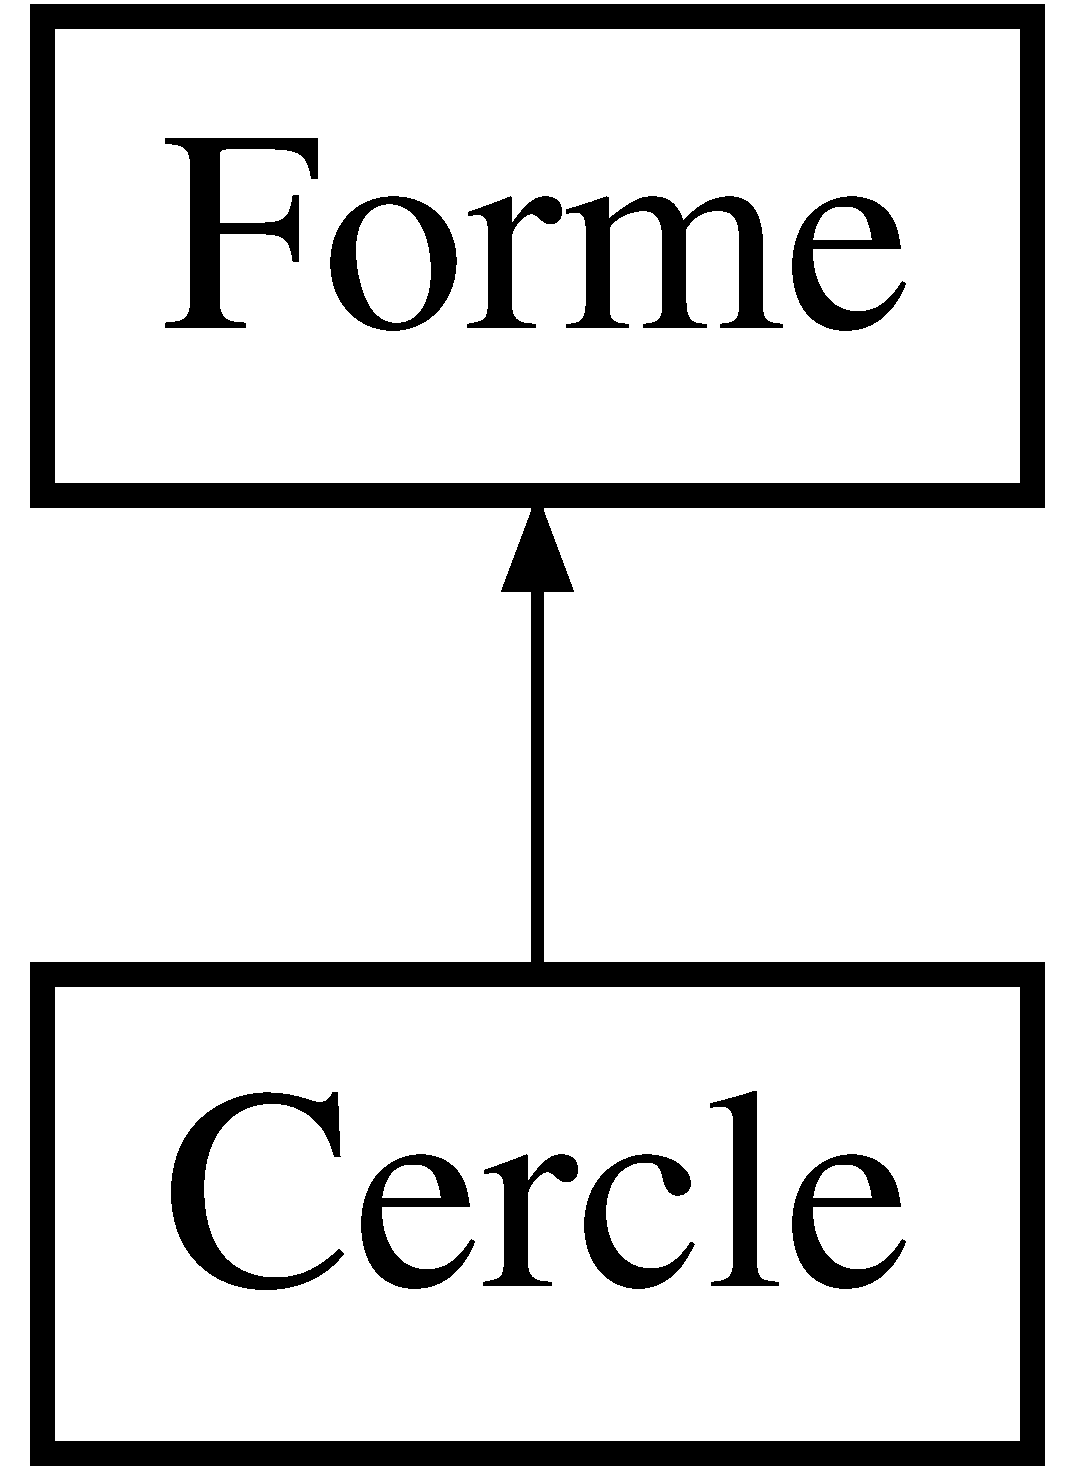
\includegraphics[height=2.000000cm]{class_cercle}
\end{center}
\end{figure}
\subsection*{Public Member Functions}
\begin{DoxyCompactItemize}
\item 
\hyperlink{class_cercle_a86c13d359c4446b4f0ccad491b86c72f}{Cercle} (const \hyperlink{class_vecteur2_d}{Vecteur2D} \&centre, double rayon, const \hyperlink{class_couleur}{Couleur} \&coul=\hyperlink{class_couleur}{Couleur}())
\begin{DoxyCompactList}\small\item\em Constructeur � partir du centre, d\textquotesingle{}un rayon et d\textquotesingle{}une couleur. \end{DoxyCompactList}\item 
\hyperlink{class_cercle_a5711ce1dc4faf72a6b02cddbb9c618cd}{Cercle} (const \hyperlink{class_cercle}{Cercle} \&obj)
\begin{DoxyCompactList}\small\item\em Constructeur par recopie d\textquotesingle{}un cercle. \end{DoxyCompactList}\item 
\hyperlink{class_cercle_a56cf93b56461ba960b822b9a095b09ad}{$\sim$\+Cercle} ()
\begin{DoxyCompactList}\small\item\em Destructeur. \end{DoxyCompactList}\item 
\hyperlink{class_vecteur2_d}{Vecteur2D} \hyperlink{class_cercle_afbf26df611767f7b1cc22904fd844932}{get\+Centre} () const
\begin{DoxyCompactList}\small\item\em Getter pour r�cup�rer le centre du cercle. \end{DoxyCompactList}\item 
void \hyperlink{class_cercle_ac32cf43ab91937caf98d1a130f99937c}{set\+Centre} (const \hyperlink{class_vecteur2_d}{Vecteur2D} \&centre)
\begin{DoxyCompactList}\small\item\em Setter pour modifier le centre du cercle. \end{DoxyCompactList}\item 
double \hyperlink{class_cercle_abc1c953fd5ef431158e89dc8344b1de1}{get\+Rayon} () const
\begin{DoxyCompactList}\small\item\em Getter pour r�cup�rer le rayon du cercle. \end{DoxyCompactList}\item 
void \hyperlink{class_cercle_ab166965772a83365ac4b7514c0089434}{set\+Rayon} (double rayon)
\begin{DoxyCompactList}\small\item\em Setter pour modifier le rayon du cercle. \end{DoxyCompactList}\item 
\hyperlink{class_cercle_a01dfce2b49afb0dcb5bd176d4145b71a}{operator string} () const
\begin{DoxyCompactList}\small\item\em Surcharge de l\textquotesingle{}op�rateur de onversion en string. \end{DoxyCompactList}\item 
bool \hyperlink{class_cercle_a747442744a4d31ab753924b1fa3cad6a}{operator==} (const \hyperlink{class_cercle}{Cercle} \&objet) const
\begin{DoxyCompactList}\small\item\em Surcharge de l\textquotesingle{}op�rateur ==. \end{DoxyCompactList}\item 
bool \hyperlink{class_cercle_a718965509a0cbd120a5ffc513da21ac9}{operator!=} (const \hyperlink{class_cercle}{Cercle} \&objet) const
\begin{DoxyCompactList}\small\item\em Surcharge de l\textquotesingle{}op�rateur !=. \end{DoxyCompactList}\item 
const \hyperlink{class_cercle}{Cercle} \& \hyperlink{class_cercle_a83def4735f011dd4ebc18a4e6fc22a7e}{operator=} (const \hyperlink{class_cercle}{Cercle} \&obj)
\begin{DoxyCompactList}\small\item\em Surcharge de l\textquotesingle{}op�rateur =. \end{DoxyCompactList}\item 
const double \hyperlink{class_cercle_a2477495263095a5553f2bcfa524f03ac}{get\+Aire} () const
\begin{DoxyCompactList}\small\item\em Getter pour r�cup�rer l\textquotesingle{}aire du cercle. \end{DoxyCompactList}\item 
\hyperlink{class_forme}{Forme} $\ast$ \hyperlink{class_cercle_a56073052a84c4b8e04124692e6dc58f5}{clone} () const
\begin{DoxyCompactList}\small\item\em Clone un cercle. \end{DoxyCompactList}\item 
void \hyperlink{class_cercle_a41c2ecef959a6273a08d44806351f0f4}{homothetie} (const \hyperlink{class_vecteur2_d}{Vecteur2D} \&vect\+Homotethie, double k)
\begin{DoxyCompactList}\small\item\em Effectue une homot�thie sur le cercle qui modifie directement le cercle. \end{DoxyCompactList}\item 
void \hyperlink{class_cercle_aec369809aab0faf3adc93c62e6acc06c}{translation} (const \hyperlink{class_vecteur2_d}{Vecteur2D} \&vect\+Translation)
\begin{DoxyCompactList}\small\item\em Effectue une translation sur le cercle qui modifie directement le cercle. \end{DoxyCompactList}\item 
void \hyperlink{class_cercle_a6cabe637a245d902e5bfe7d82efd493f}{rotation} (const \hyperlink{class_vecteur2_d}{Vecteur2D} \&vect\+Centre, double angle)
\begin{DoxyCompactList}\small\item\em Effectue une rotation sur le cercle qui modifie directement le cercle. \end{DoxyCompactList}\item 
ostream \& \hyperlink{class_cercle_a80410c399a44cfa15bd2fd19df8f3648}{print} (ostream \&flux) const
\begin{DoxyCompactList}\small\item\em Affiche les informations sur le cercle. \end{DoxyCompactList}\item 
void \hyperlink{class_cercle_a681df3cd077879881755a727b950a263}{accepte\+Sauvegarder} (const \hyperlink{class_visiteur_sauv_t_x_t}{Visiteur\+Sauv\+T\+XT} $\ast$v) const
\begin{DoxyCompactList}\small\item\em Appelle la m�thode visite du visiteur de sauvegarde correpondant au cercle. \end{DoxyCompactList}\item 
void \hyperlink{class_cercle_a2d3d99149647f033b6f8f470c9a1f53f}{dessiner} (const \hyperlink{class_visiteur_dessin}{Visiteur\+Dessin} $\ast$v) const
\begin{DoxyCompactList}\small\item\em Appelle la m�thode visite du visiteur de dessin correpondant au cercle. \end{DoxyCompactList}\end{DoxyCompactItemize}


\subsection{Constructor \& Destructor Documentation}
\mbox{\Hypertarget{class_cercle_a86c13d359c4446b4f0ccad491b86c72f}\label{class_cercle_a86c13d359c4446b4f0ccad491b86c72f}} 
\index{Cercle@{Cercle}!Cercle@{Cercle}}
\index{Cercle@{Cercle}!Cercle@{Cercle}}
\subsubsection{\texorpdfstring{Cercle()}{Cercle()}\hspace{0.1cm}{\footnotesize\ttfamily [1/2]}}
{\footnotesize\ttfamily Cercle\+::\+Cercle (\begin{DoxyParamCaption}\item[{const \hyperlink{class_vecteur2_d}{Vecteur2D} \&}]{centre,  }\item[{double}]{rayon,  }\item[{const \hyperlink{class_couleur}{Couleur} \&}]{coul = {\ttfamily \hyperlink{class_couleur}{Couleur}()} }\end{DoxyParamCaption})}



Constructeur � partir du centre, d\textquotesingle{}un rayon et d\textquotesingle{}une couleur. 

La couleur est mise par d�faut avec le constructeur par d�faut \hyperlink{class_couleur}{Couleur}. 
\begin{DoxyParams}{Parameters}
{\em centre} & \hyperlink{class_vecteur2_d}{Vecteur2D} \\
\hline
{\em rayon} & R�el \\
\hline
{\em coul} & \hyperlink{class_couleur}{Couleur} du cercle \\
\hline
\end{DoxyParams}
\mbox{\Hypertarget{class_cercle_a5711ce1dc4faf72a6b02cddbb9c618cd}\label{class_cercle_a5711ce1dc4faf72a6b02cddbb9c618cd}} 
\index{Cercle@{Cercle}!Cercle@{Cercle}}
\index{Cercle@{Cercle}!Cercle@{Cercle}}
\subsubsection{\texorpdfstring{Cercle()}{Cercle()}\hspace{0.1cm}{\footnotesize\ttfamily [2/2]}}
{\footnotesize\ttfamily Cercle\+::\+Cercle (\begin{DoxyParamCaption}\item[{const \hyperlink{class_cercle}{Cercle} \&}]{obj }\end{DoxyParamCaption})}



Constructeur par recopie d\textquotesingle{}un cercle. 


\begin{DoxyParams}{Parameters}
{\em obj} & \hyperlink{class_cercle}{Cercle} � recopier \\
\hline
\end{DoxyParams}
\mbox{\Hypertarget{class_cercle_a56cf93b56461ba960b822b9a095b09ad}\label{class_cercle_a56cf93b56461ba960b822b9a095b09ad}} 
\index{Cercle@{Cercle}!````~Cercle@{$\sim$\+Cercle}}
\index{````~Cercle@{$\sim$\+Cercle}!Cercle@{Cercle}}
\subsubsection{\texorpdfstring{$\sim$\+Cercle()}{~Cercle()}}
{\footnotesize\ttfamily Cercle\+::$\sim$\+Cercle (\begin{DoxyParamCaption}{ }\end{DoxyParamCaption})}



Destructeur. 



\subsection{Member Function Documentation}
\mbox{\Hypertarget{class_cercle_a681df3cd077879881755a727b950a263}\label{class_cercle_a681df3cd077879881755a727b950a263}} 
\index{Cercle@{Cercle}!accepte\+Sauvegarder@{accepte\+Sauvegarder}}
\index{accepte\+Sauvegarder@{accepte\+Sauvegarder}!Cercle@{Cercle}}
\subsubsection{\texorpdfstring{accepte\+Sauvegarder()}{accepteSauvegarder()}}
{\footnotesize\ttfamily void Cercle\+::accepte\+Sauvegarder (\begin{DoxyParamCaption}\item[{const \hyperlink{class_visiteur_sauv_t_x_t}{Visiteur\+Sauv\+T\+XT} $\ast$}]{v }\end{DoxyParamCaption}) const\hspace{0.3cm}{\ttfamily [virtual]}}



Appelle la m�thode visite du visiteur de sauvegarde correpondant au cercle. 


\begin{DoxyParams}{Parameters}
{\em v} & Pointeur sur le visiteur de sauvegarde \\
\hline
\end{DoxyParams}


Implements \hyperlink{class_forme_a7be10bca98001dc368adc3a3e93d0f48}{Forme}.

\mbox{\Hypertarget{class_cercle_a56073052a84c4b8e04124692e6dc58f5}\label{class_cercle_a56073052a84c4b8e04124692e6dc58f5}} 
\index{Cercle@{Cercle}!clone@{clone}}
\index{clone@{clone}!Cercle@{Cercle}}
\subsubsection{\texorpdfstring{clone()}{clone()}}
{\footnotesize\ttfamily \hyperlink{class_forme}{Forme} $\ast$ Cercle\+::clone (\begin{DoxyParamCaption}{ }\end{DoxyParamCaption}) const\hspace{0.3cm}{\ttfamily [virtual]}}



Clone un cercle. 

M�thode virtuelle pure que l\textquotesingle{}on red�finit ici \begin{DoxyReturn}{Returns}
Forme$\ast$ Un pointeur sur une \hyperlink{class_forme}{Forme} (ici un cercle) 
\end{DoxyReturn}


Implements \hyperlink{class_forme_a226750dc3f772514fe58e1dc16f3d0d5}{Forme}.

\mbox{\Hypertarget{class_cercle_a2d3d99149647f033b6f8f470c9a1f53f}\label{class_cercle_a2d3d99149647f033b6f8f470c9a1f53f}} 
\index{Cercle@{Cercle}!dessiner@{dessiner}}
\index{dessiner@{dessiner}!Cercle@{Cercle}}
\subsubsection{\texorpdfstring{dessiner()}{dessiner()}}
{\footnotesize\ttfamily void Cercle\+::dessiner (\begin{DoxyParamCaption}\item[{const \hyperlink{class_visiteur_dessin}{Visiteur\+Dessin} $\ast$}]{v }\end{DoxyParamCaption}) const\hspace{0.3cm}{\ttfamily [virtual]}}



Appelle la m�thode visite du visiteur de dessin correpondant au cercle. 


\begin{DoxyParams}{Parameters}
{\em v} & Pointeur sur le visiteur de dessin \\
\hline
\end{DoxyParams}


Implements \hyperlink{class_forme_a8cd4879a6a5751cbf6d3bbbfbec41566}{Forme}.

\mbox{\Hypertarget{class_cercle_a2477495263095a5553f2bcfa524f03ac}\label{class_cercle_a2477495263095a5553f2bcfa524f03ac}} 
\index{Cercle@{Cercle}!get\+Aire@{get\+Aire}}
\index{get\+Aire@{get\+Aire}!Cercle@{Cercle}}
\subsubsection{\texorpdfstring{get\+Aire()}{getAire()}}
{\footnotesize\ttfamily const double Cercle\+::get\+Aire (\begin{DoxyParamCaption}{ }\end{DoxyParamCaption}) const\hspace{0.3cm}{\ttfamily [virtual]}}



Getter pour r�cup�rer l\textquotesingle{}aire du cercle. 

\begin{DoxyReturn}{Returns}
R�el Correspondant � l\textquotesingle{}aire du cercle 
\end{DoxyReturn}


Implements \hyperlink{class_forme_adf4346150d8f734d7a48f7661e30cab4}{Forme}.

\mbox{\Hypertarget{class_cercle_afbf26df611767f7b1cc22904fd844932}\label{class_cercle_afbf26df611767f7b1cc22904fd844932}} 
\index{Cercle@{Cercle}!get\+Centre@{get\+Centre}}
\index{get\+Centre@{get\+Centre}!Cercle@{Cercle}}
\subsubsection{\texorpdfstring{get\+Centre()}{getCentre()}}
{\footnotesize\ttfamily \hyperlink{class_vecteur2_d}{Vecteur2D} Cercle\+::get\+Centre (\begin{DoxyParamCaption}{ }\end{DoxyParamCaption}) const}



Getter pour r�cup�rer le centre du cercle. 

\begin{DoxyReturn}{Returns}
\hyperlink{class_vecteur2_d}{Vecteur2D} Le centre du cercle 
\end{DoxyReturn}
\mbox{\Hypertarget{class_cercle_abc1c953fd5ef431158e89dc8344b1de1}\label{class_cercle_abc1c953fd5ef431158e89dc8344b1de1}} 
\index{Cercle@{Cercle}!get\+Rayon@{get\+Rayon}}
\index{get\+Rayon@{get\+Rayon}!Cercle@{Cercle}}
\subsubsection{\texorpdfstring{get\+Rayon()}{getRayon()}}
{\footnotesize\ttfamily double Cercle\+::get\+Rayon (\begin{DoxyParamCaption}{ }\end{DoxyParamCaption}) const}



Getter pour r�cup�rer le rayon du cercle. 

\begin{DoxyReturn}{Returns}
R�el Le rayon du cercle 
\end{DoxyReturn}
\mbox{\Hypertarget{class_cercle_a41c2ecef959a6273a08d44806351f0f4}\label{class_cercle_a41c2ecef959a6273a08d44806351f0f4}} 
\index{Cercle@{Cercle}!homothetie@{homothetie}}
\index{homothetie@{homothetie}!Cercle@{Cercle}}
\subsubsection{\texorpdfstring{homothetie()}{homothetie()}}
{\footnotesize\ttfamily void Cercle\+::homothetie (\begin{DoxyParamCaption}\item[{const \hyperlink{class_vecteur2_d}{Vecteur2D} \&}]{vect\+Homotethie,  }\item[{double}]{k }\end{DoxyParamCaption})\hspace{0.3cm}{\ttfamily [virtual]}}



Effectue une homot�thie sur le cercle qui modifie directement le cercle. 


\begin{DoxyParams}{Parameters}
{\em vect\+Homotethie} & \hyperlink{class_vecteur2_d}{Vecteur2D} \\
\hline
{\em k} & R�el \\
\hline
\end{DoxyParams}


Implements \hyperlink{class_forme_aeaae98ea3de8523de9ba9093e19779d8}{Forme}.

\mbox{\Hypertarget{class_cercle_a01dfce2b49afb0dcb5bd176d4145b71a}\label{class_cercle_a01dfce2b49afb0dcb5bd176d4145b71a}} 
\index{Cercle@{Cercle}!operator string@{operator string}}
\index{operator string@{operator string}!Cercle@{Cercle}}
\subsubsection{\texorpdfstring{operator string()}{operator string()}}
{\footnotesize\ttfamily Cercle\+::operator string (\begin{DoxyParamCaption}{ }\end{DoxyParamCaption}) const\hspace{0.3cm}{\ttfamily [virtual]}}



Surcharge de l\textquotesingle{}op�rateur de onversion en string. 

Convertit un \hyperlink{class_cercle}{Cercle} en string 

Reimplemented from \hyperlink{class_forme_a809375f023f0f19227f3e3821ee56731}{Forme}.

\mbox{\Hypertarget{class_cercle_a718965509a0cbd120a5ffc513da21ac9}\label{class_cercle_a718965509a0cbd120a5ffc513da21ac9}} 
\index{Cercle@{Cercle}!operator"!=@{operator"!=}}
\index{operator"!=@{operator"!=}!Cercle@{Cercle}}
\subsubsection{\texorpdfstring{operator"!=()}{operator!=()}}
{\footnotesize\ttfamily bool Cercle\+::operator!= (\begin{DoxyParamCaption}\item[{const \hyperlink{class_cercle}{Cercle} \&}]{objet }\end{DoxyParamCaption}) const}



Surcharge de l\textquotesingle{}op�rateur !=. 

Utilise == pour comparer si deux cercles sont diff�rents 
\begin{DoxyParams}{Parameters}
{\em objet} & \hyperlink{class_cercle}{Cercle} � comparer \\
\hline
\end{DoxyParams}
\begin{DoxyReturn}{Returns}
bool Un bool�en vrai si les deux cercles sont diff�rents, faux sinon 
\end{DoxyReturn}
\mbox{\Hypertarget{class_cercle_a83def4735f011dd4ebc18a4e6fc22a7e}\label{class_cercle_a83def4735f011dd4ebc18a4e6fc22a7e}} 
\index{Cercle@{Cercle}!operator=@{operator=}}
\index{operator=@{operator=}!Cercle@{Cercle}}
\subsubsection{\texorpdfstring{operator=()}{operator=()}}
{\footnotesize\ttfamily const \hyperlink{class_cercle}{Cercle} \& Cercle\+::operator= (\begin{DoxyParamCaption}\item[{const \hyperlink{class_cercle}{Cercle} \&}]{obj }\end{DoxyParamCaption})}



Surcharge de l\textquotesingle{}op�rateur =. 

Affecte � un cercle les valeurs d\textquotesingle{}un autre cercle 
\begin{DoxyParams}{Parameters}
{\em obj} & \hyperlink{class_cercle}{Cercle} � copier \\
\hline
\end{DoxyParams}
\mbox{\Hypertarget{class_cercle_a747442744a4d31ab753924b1fa3cad6a}\label{class_cercle_a747442744a4d31ab753924b1fa3cad6a}} 
\index{Cercle@{Cercle}!operator==@{operator==}}
\index{operator==@{operator==}!Cercle@{Cercle}}
\subsubsection{\texorpdfstring{operator==()}{operator==()}}
{\footnotesize\ttfamily bool Cercle\+::operator== (\begin{DoxyParamCaption}\item[{const \hyperlink{class_cercle}{Cercle} \&}]{objet }\end{DoxyParamCaption}) const}



Surcharge de l\textquotesingle{}op�rateur ==. 

Teste si deux cercles sont identiques 
\begin{DoxyParams}{Parameters}
{\em objet} & \hyperlink{class_cercle}{Cercle} � comparer \\
\hline
\end{DoxyParams}
\begin{DoxyReturn}{Returns}
bool Un bool�en vrai si les deux cercles sont identiques, faux sinon 
\end{DoxyReturn}
\mbox{\Hypertarget{class_cercle_a80410c399a44cfa15bd2fd19df8f3648}\label{class_cercle_a80410c399a44cfa15bd2fd19df8f3648}} 
\index{Cercle@{Cercle}!print@{print}}
\index{print@{print}!Cercle@{Cercle}}
\subsubsection{\texorpdfstring{print()}{print()}}
{\footnotesize\ttfamily ostream \& Cercle\+::print (\begin{DoxyParamCaption}\item[{ostream \&}]{flux }\end{DoxyParamCaption}) const\hspace{0.3cm}{\ttfamily [virtual]}}



Affiche les informations sur le cercle. 


\begin{DoxyParams}{Parameters}
{\em flux} & Flux de sortie \\
\hline
\end{DoxyParams}
\begin{DoxyReturn}{Returns}
ostream Un flux de sortie 
\end{DoxyReturn}


Reimplemented from \hyperlink{class_forme_a348a12ae03fe2167ffd586f4deae6c76}{Forme}.

\mbox{\Hypertarget{class_cercle_a6cabe637a245d902e5bfe7d82efd493f}\label{class_cercle_a6cabe637a245d902e5bfe7d82efd493f}} 
\index{Cercle@{Cercle}!rotation@{rotation}}
\index{rotation@{rotation}!Cercle@{Cercle}}
\subsubsection{\texorpdfstring{rotation()}{rotation()}}
{\footnotesize\ttfamily void Cercle\+::rotation (\begin{DoxyParamCaption}\item[{const \hyperlink{class_vecteur2_d}{Vecteur2D} \&}]{vect\+Centre,  }\item[{double}]{angle }\end{DoxyParamCaption})\hspace{0.3cm}{\ttfamily [virtual]}}



Effectue une rotation sur le cercle qui modifie directement le cercle. 


\begin{DoxyParams}{Parameters}
{\em vect\+Centre} & \hyperlink{class_vecteur2_d}{Vecteur2D} \\
\hline
{\em angle} & R�el \\
\hline
\end{DoxyParams}


Implements \hyperlink{class_forme_af17c4156d00281b4b62d8c27dcb75569}{Forme}.

\mbox{\Hypertarget{class_cercle_ac32cf43ab91937caf98d1a130f99937c}\label{class_cercle_ac32cf43ab91937caf98d1a130f99937c}} 
\index{Cercle@{Cercle}!set\+Centre@{set\+Centre}}
\index{set\+Centre@{set\+Centre}!Cercle@{Cercle}}
\subsubsection{\texorpdfstring{set\+Centre()}{setCentre()}}
{\footnotesize\ttfamily void Cercle\+::set\+Centre (\begin{DoxyParamCaption}\item[{const \hyperlink{class_vecteur2_d}{Vecteur2D} \&}]{centre }\end{DoxyParamCaption})}



Setter pour modifier le centre du cercle. 


\begin{DoxyParams}{Parameters}
{\em centre} & \hyperlink{class_vecteur2_d}{Vecteur2D} correspondant au cercle \\
\hline
\end{DoxyParams}
\mbox{\Hypertarget{class_cercle_ab166965772a83365ac4b7514c0089434}\label{class_cercle_ab166965772a83365ac4b7514c0089434}} 
\index{Cercle@{Cercle}!set\+Rayon@{set\+Rayon}}
\index{set\+Rayon@{set\+Rayon}!Cercle@{Cercle}}
\subsubsection{\texorpdfstring{set\+Rayon()}{setRayon()}}
{\footnotesize\ttfamily void Cercle\+::set\+Rayon (\begin{DoxyParamCaption}\item[{double}]{rayon }\end{DoxyParamCaption})}



Setter pour modifier le rayon du cercle. 


\begin{DoxyParams}{Parameters}
{\em rayon} & R�el \\
\hline
\end{DoxyParams}
\mbox{\Hypertarget{class_cercle_aec369809aab0faf3adc93c62e6acc06c}\label{class_cercle_aec369809aab0faf3adc93c62e6acc06c}} 
\index{Cercle@{Cercle}!translation@{translation}}
\index{translation@{translation}!Cercle@{Cercle}}
\subsubsection{\texorpdfstring{translation()}{translation()}}
{\footnotesize\ttfamily void Cercle\+::translation (\begin{DoxyParamCaption}\item[{const \hyperlink{class_vecteur2_d}{Vecteur2D} \&}]{vect\+Translation }\end{DoxyParamCaption})\hspace{0.3cm}{\ttfamily [virtual]}}



Effectue une translation sur le cercle qui modifie directement le cercle. 


\begin{DoxyParams}{Parameters}
{\em vect\+Translation} & \hyperlink{class_vecteur2_d}{Vecteur2D} \\
\hline
\end{DoxyParams}


Implements \hyperlink{class_forme_ad156a02098ef453b09919b2a3156f607}{Forme}.



The documentation for this class was generated from the following files\+:\begin{DoxyCompactItemize}
\item 
C\+:/\+Users/\+Quentin Fixe/\+Desktop/\+P\+P\+I\+L-\/master/\+C\+L\+I\+E\+N\+T/\hyperlink{_cercle_8h}{Cercle.\+h}\item 
C\+:/\+Users/\+Quentin Fixe/\+Desktop/\+P\+P\+I\+L-\/master/\+C\+L\+I\+E\+N\+T/\hyperlink{_cercle_8cpp}{Cercle.\+cpp}\end{DoxyCompactItemize}

\hypertarget{class_charger_forme}{}\section{Charger\+Forme Class Reference}
\label{class_charger_forme}\index{Charger\+Forme@{Charger\+Forme}}


{\ttfamily \#include $<$Charger\+Forme.\+h$>$}

Inheritance diagram for Charger\+Forme\+:\begin{figure}[H]
\begin{center}
\leavevmode
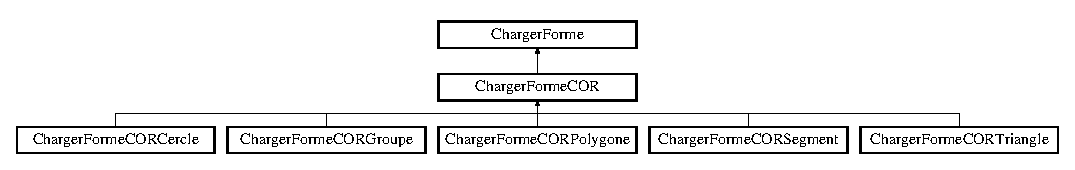
\includegraphics[height=1.836066cm]{class_charger_forme}
\end{center}
\end{figure}
\subsection*{Public Member Functions}
\begin{DoxyCompactItemize}
\item 
virtual \hyperlink{class_forme}{Forme} $\ast$ \hyperlink{class_charger_forme_a0564f02729aa97751342d399e8914a87}{charger} (const string \&id\+Forme, const string \&info=\char`\"{}\char`\"{}) const =0
\begin{DoxyCompactList}\small\item\em M�thode virtuelle pure qui va appeler un expert pour charger la forme, si l\textquotesingle{}expert ne sait pas r�soudre le probl�me alors on passe � l\textquotesingle{}expert suivant \textbackslash{} param id\+Forme Chaine de cract�re correspondant � l\textquotesingle{}identifiant de la forme � charger. \end{DoxyCompactList}\end{DoxyCompactItemize}


\subsection{Member Function Documentation}
\mbox{\Hypertarget{class_charger_forme_a0564f02729aa97751342d399e8914a87}\label{class_charger_forme_a0564f02729aa97751342d399e8914a87}} 
\index{Charger\+Forme@{Charger\+Forme}!charger@{charger}}
\index{charger@{charger}!Charger\+Forme@{Charger\+Forme}}
\subsubsection{\texorpdfstring{charger()}{charger()}}
{\footnotesize\ttfamily virtual \hyperlink{class_forme}{Forme}$\ast$ Charger\+Forme\+::charger (\begin{DoxyParamCaption}\item[{const string \&}]{id\+Forme,  }\item[{const string \&}]{info = {\ttfamily \char`\"{}\char`\"{}} }\end{DoxyParamCaption}) const\hspace{0.3cm}{\ttfamily [pure virtual]}}



M�thode virtuelle pure qui va appeler un expert pour charger la forme, si l\textquotesingle{}expert ne sait pas r�soudre le probl�me alors on passe � l\textquotesingle{}expert suivant \textbackslash{} param id\+Forme Chaine de cract�re correspondant � l\textquotesingle{}identifiant de la forme � charger. 


\begin{DoxyParams}{Parameters}
{\em info} & Chaine de caract�re contenant les informations de la forme � charger (vide par d�faut) \\
\hline
\end{DoxyParams}
\begin{DoxyReturn}{Returns}
Forme$\ast$ Pointeur sur la forme charg�e 
\end{DoxyReturn}


Implemented in \hyperlink{class_charger_forme_c_o_r_aa40ed5e3df01527bcaaf61c5bb56bd65}{Charger\+Forme\+C\+OR}.



The documentation for this class was generated from the following file\+:\begin{DoxyCompactItemize}
\item 
C\+:/\+Users/\+Quentin Fixe/\+Desktop/\+P\+P\+I\+L-\/master/\+C\+L\+I\+E\+N\+T/\hyperlink{_charger_forme_8h}{Charger\+Forme.\+h}\end{DoxyCompactItemize}

\hypertarget{class_charger_forme_c_o_r}{}\section{Charger\+Forme\+C\+OR Class Reference}
\label{class_charger_forme_c_o_r}\index{Charger\+Forme\+C\+OR@{Charger\+Forme\+C\+OR}}


{\ttfamily \#include $<$Charger\+Forme\+C\+O\+R.\+h$>$}

Inheritance diagram for Charger\+Forme\+C\+OR\+:\begin{figure}[H]
\begin{center}
\leavevmode
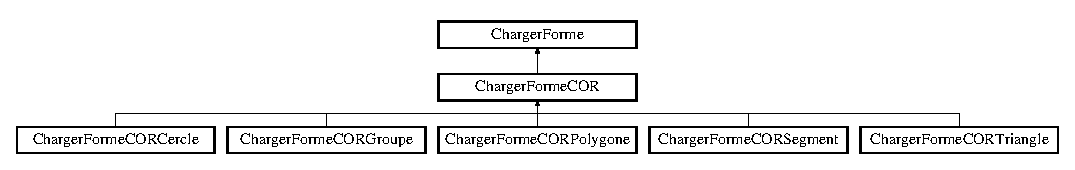
\includegraphics[height=1.836066cm]{class_charger_forme_c_o_r}
\end{center}
\end{figure}
\subsection*{Public Member Functions}
\begin{DoxyCompactItemize}
\item 
\hyperlink{class_charger_forme_c_o_r_a95609cb9640074329ce2ff8ac22d622f}{Charger\+Forme\+C\+OR} (\hyperlink{class_charger_forme_c_o_r}{Charger\+Forme\+C\+OR} $\ast$suivant)
\begin{DoxyCompactList}\small\item\em Constructeur � partir d\textquotesingle{}un pointeur sur l\textquotesingle{}expert suivant. \end{DoxyCompactList}\item 
\hyperlink{class_forme}{Forme} $\ast$ \hyperlink{class_charger_forme_c_o_r_aa40ed5e3df01527bcaaf61c5bb56bd65}{charger} (const string \&id\+Forme, const string \&info=\char`\"{}\char`\"{}) const
\begin{DoxyCompactList}\small\item\em Appelle un expert pour charger la forme, si l\textquotesingle{}expert ne sait pas r�soudre le probl�me alors on passe � l\textquotesingle{}expert suivant \textbackslash{} param id\+Forme Chaine de cract�re correspondant � l\textquotesingle{}identifiant de la forme � charger. \end{DoxyCompactList}\item 
virtual const string \hyperlink{class_charger_forme_c_o_r_ae740eabcd9b3cc3809c1fe5ffd0100a1}{get\+Type\+Forme} () const =0
\begin{DoxyCompactList}\small\item\em M�thode virtuelle pure qui retourne le type de la forme. \end{DoxyCompactList}\item 
virtual \hyperlink{class_forme}{Forme} $\ast$ \hyperlink{class_charger_forme_c_o_r_a1d9563c3a1ff9d6d86aa87a83bdaf8da}{traiter\+Demande} (const string \&info\+Forme) const =0
\begin{DoxyCompactList}\small\item\em M�thode virtuelle pure. Extrait les donn�es d\textquotesingle{}une forme � partir d\textquotesingle{}une chaine de caract�res. \end{DoxyCompactList}\end{DoxyCompactItemize}
\subsection*{Protected Member Functions}
\begin{DoxyCompactItemize}
\item 
string \hyperlink{class_charger_forme_c_o_r_a582e95ff92f06d2c45e6c46f09151e36}{get\+Info\+Forme} (const string \&id\+Forme) const
\begin{DoxyCompactList}\small\item\em R�cup�re les informations d\textquotesingle{}une forme en fonction de son identifiant. \end{DoxyCompactList}\item 
\hyperlink{class_vecteur2_d}{Vecteur2D} \hyperlink{class_charger_forme_c_o_r_a5b1cd8aabcc803143234a7034047a62b}{string\+To\+Point} (const string \&info\+Point) const
\begin{DoxyCompactList}\small\item\em Convertion d\textquotesingle{}une chaine de caract�res correspondant � un point en un \hyperlink{class_vecteur2_d}{Vecteur2D}. \end{DoxyCompactList}\end{DoxyCompactItemize}


\subsection{Constructor \& Destructor Documentation}
\mbox{\Hypertarget{class_charger_forme_c_o_r_a95609cb9640074329ce2ff8ac22d622f}\label{class_charger_forme_c_o_r_a95609cb9640074329ce2ff8ac22d622f}} 
\index{Charger\+Forme\+C\+OR@{Charger\+Forme\+C\+OR}!Charger\+Forme\+C\+OR@{Charger\+Forme\+C\+OR}}
\index{Charger\+Forme\+C\+OR@{Charger\+Forme\+C\+OR}!Charger\+Forme\+C\+OR@{Charger\+Forme\+C\+OR}}
\subsubsection{\texorpdfstring{Charger\+Forme\+C\+O\+R()}{ChargerFormeCOR()}}
{\footnotesize\ttfamily Charger\+Forme\+C\+O\+R\+::\+Charger\+Forme\+C\+OR (\begin{DoxyParamCaption}\item[{\hyperlink{class_charger_forme_c_o_r}{Charger\+Forme\+C\+OR} $\ast$}]{suivant }\end{DoxyParamCaption})}



Constructeur � partir d\textquotesingle{}un pointeur sur l\textquotesingle{}expert suivant. 


\begin{DoxyParams}{Parameters}
{\em suivant} & Pointeur sur l\textquotesingle{}expert suivant \\
\hline
\end{DoxyParams}


\subsection{Member Function Documentation}
\mbox{\Hypertarget{class_charger_forme_c_o_r_aa40ed5e3df01527bcaaf61c5bb56bd65}\label{class_charger_forme_c_o_r_aa40ed5e3df01527bcaaf61c5bb56bd65}} 
\index{Charger\+Forme\+C\+OR@{Charger\+Forme\+C\+OR}!charger@{charger}}
\index{charger@{charger}!Charger\+Forme\+C\+OR@{Charger\+Forme\+C\+OR}}
\subsubsection{\texorpdfstring{charger()}{charger()}}
{\footnotesize\ttfamily \hyperlink{class_forme}{Forme} $\ast$ Charger\+Forme\+C\+O\+R\+::charger (\begin{DoxyParamCaption}\item[{const string \&}]{id\+Forme,  }\item[{const string \&}]{info = {\ttfamily \char`\"{}\char`\"{}} }\end{DoxyParamCaption}) const\hspace{0.3cm}{\ttfamily [virtual]}}



Appelle un expert pour charger la forme, si l\textquotesingle{}expert ne sait pas r�soudre le probl�me alors on passe � l\textquotesingle{}expert suivant \textbackslash{} param id\+Forme Chaine de cract�re correspondant � l\textquotesingle{}identifiant de la forme � charger. 


\begin{DoxyParams}{Parameters}
{\em info} & Chaine de caract�re contenant les informations de la forme � charger (vide par d�faut) \\
\hline
\end{DoxyParams}
\begin{DoxyReturn}{Returns}
Forme$\ast$ Pointeur sur la forme charg�e 
\end{DoxyReturn}


Implements \hyperlink{class_charger_forme_a0564f02729aa97751342d399e8914a87}{Charger\+Forme}.

\mbox{\Hypertarget{class_charger_forme_c_o_r_a582e95ff92f06d2c45e6c46f09151e36}\label{class_charger_forme_c_o_r_a582e95ff92f06d2c45e6c46f09151e36}} 
\index{Charger\+Forme\+C\+OR@{Charger\+Forme\+C\+OR}!get\+Info\+Forme@{get\+Info\+Forme}}
\index{get\+Info\+Forme@{get\+Info\+Forme}!Charger\+Forme\+C\+OR@{Charger\+Forme\+C\+OR}}
\subsubsection{\texorpdfstring{get\+Info\+Forme()}{getInfoForme()}}
{\footnotesize\ttfamily string Charger\+Forme\+C\+O\+R\+::get\+Info\+Forme (\begin{DoxyParamCaption}\item[{const string \&}]{id\+Forme }\end{DoxyParamCaption}) const\hspace{0.3cm}{\ttfamily [protected]}}



R�cup�re les informations d\textquotesingle{}une forme en fonction de son identifiant. 


\begin{DoxyParams}{Parameters}
{\em id\+Forme} & Identifiant de la forme \\
\hline
\end{DoxyParams}
\begin{DoxyReturn}{Returns}
string Informations de la forme 
\end{DoxyReturn}
\mbox{\Hypertarget{class_charger_forme_c_o_r_ae740eabcd9b3cc3809c1fe5ffd0100a1}\label{class_charger_forme_c_o_r_ae740eabcd9b3cc3809c1fe5ffd0100a1}} 
\index{Charger\+Forme\+C\+OR@{Charger\+Forme\+C\+OR}!get\+Type\+Forme@{get\+Type\+Forme}}
\index{get\+Type\+Forme@{get\+Type\+Forme}!Charger\+Forme\+C\+OR@{Charger\+Forme\+C\+OR}}
\subsubsection{\texorpdfstring{get\+Type\+Forme()}{getTypeForme()}}
{\footnotesize\ttfamily virtual const string Charger\+Forme\+C\+O\+R\+::get\+Type\+Forme (\begin{DoxyParamCaption}{ }\end{DoxyParamCaption}) const\hspace{0.3cm}{\ttfamily [pure virtual]}}



M�thode virtuelle pure qui retourne le type de la forme. 

\begin{DoxyReturn}{Returns}
string Type de la forme 
\end{DoxyReturn}


Implemented in \hyperlink{class_charger_forme_c_o_r_cercle_a4ca5a036a26641c2636d376f51659172}{Charger\+Forme\+C\+O\+R\+Cercle}, \hyperlink{class_charger_forme_c_o_r_groupe_a202dfd1ec95bc7a20daeb66a92452a11}{Charger\+Forme\+C\+O\+R\+Groupe}, \hyperlink{class_charger_forme_c_o_r_polygone_a8e702295e28572dc41020965255b847a}{Charger\+Forme\+C\+O\+R\+Polygone}, \hyperlink{class_charger_forme_c_o_r_segment_a88fc3dc3d1e4fb196246f5105965e285}{Charger\+Forme\+C\+O\+R\+Segment}, and \hyperlink{class_charger_forme_c_o_r_triangle_a7a0271b76c6abea8c67be2c920d72925}{Charger\+Forme\+C\+O\+R\+Triangle}.

\mbox{\Hypertarget{class_charger_forme_c_o_r_a5b1cd8aabcc803143234a7034047a62b}\label{class_charger_forme_c_o_r_a5b1cd8aabcc803143234a7034047a62b}} 
\index{Charger\+Forme\+C\+OR@{Charger\+Forme\+C\+OR}!string\+To\+Point@{string\+To\+Point}}
\index{string\+To\+Point@{string\+To\+Point}!Charger\+Forme\+C\+OR@{Charger\+Forme\+C\+OR}}
\subsubsection{\texorpdfstring{string\+To\+Point()}{stringToPoint()}}
{\footnotesize\ttfamily \hyperlink{class_vecteur2_d}{Vecteur2D} Charger\+Forme\+C\+O\+R\+::string\+To\+Point (\begin{DoxyParamCaption}\item[{const string \&}]{info\+Point }\end{DoxyParamCaption}) const\hspace{0.3cm}{\ttfamily [protected]}}



Convertion d\textquotesingle{}une chaine de caract�res correspondant � un point en un \hyperlink{class_vecteur2_d}{Vecteur2D}. 

\begin{DoxyReturn}{Returns}
\hyperlink{class_vecteur2_d}{Vecteur2D} Point converti depuis une chaine de caract�res 
\end{DoxyReturn}
\mbox{\Hypertarget{class_charger_forme_c_o_r_a1d9563c3a1ff9d6d86aa87a83bdaf8da}\label{class_charger_forme_c_o_r_a1d9563c3a1ff9d6d86aa87a83bdaf8da}} 
\index{Charger\+Forme\+C\+OR@{Charger\+Forme\+C\+OR}!traiter\+Demande@{traiter\+Demande}}
\index{traiter\+Demande@{traiter\+Demande}!Charger\+Forme\+C\+OR@{Charger\+Forme\+C\+OR}}
\subsubsection{\texorpdfstring{traiter\+Demande()}{traiterDemande()}}
{\footnotesize\ttfamily virtual \hyperlink{class_forme}{Forme}$\ast$ Charger\+Forme\+C\+O\+R\+::traiter\+Demande (\begin{DoxyParamCaption}\item[{const string \&}]{info\+Forme }\end{DoxyParamCaption}) const\hspace{0.3cm}{\ttfamily [pure virtual]}}



M�thode virtuelle pure. Extrait les donn�es d\textquotesingle{}une forme � partir d\textquotesingle{}une chaine de caract�res. 


\begin{DoxyParams}{Parameters}
{\em info\+Forme} & Chaine de caract�res correspondant aux donn�es de la forme \\
\hline
\end{DoxyParams}
\begin{DoxyReturn}{Returns}
Forme$\ast$ Un pointeur sur la forme 
\end{DoxyReturn}


Implemented in \hyperlink{class_charger_forme_c_o_r_cercle_ad65cbf0176ef4a65b44c5782646e45fa}{Charger\+Forme\+C\+O\+R\+Cercle}, \hyperlink{class_charger_forme_c_o_r_groupe_ab28f5a9e7a8fe306c98aa3f1f8b775e4}{Charger\+Forme\+C\+O\+R\+Groupe}, \hyperlink{class_charger_forme_c_o_r_polygone_a4ce89ecdaa400d4930743a8e7204b5f2}{Charger\+Forme\+C\+O\+R\+Polygone}, \hyperlink{class_charger_forme_c_o_r_segment_ac7998f4a2669a3f88dc0b204af187780}{Charger\+Forme\+C\+O\+R\+Segment}, and \hyperlink{class_charger_forme_c_o_r_triangle_aaa2b1605bb747f29a559f966754237a2}{Charger\+Forme\+C\+O\+R\+Triangle}.



The documentation for this class was generated from the following files\+:\begin{DoxyCompactItemize}
\item 
C\+:/\+Users/\+Quentin Fixe/\+Desktop/\+P\+P\+I\+L-\/master/\+C\+L\+I\+E\+N\+T/\hyperlink{_charger_forme_c_o_r_8h}{Charger\+Forme\+C\+O\+R.\+h}\item 
C\+:/\+Users/\+Quentin Fixe/\+Desktop/\+P\+P\+I\+L-\/master/\+C\+L\+I\+E\+N\+T/\hyperlink{_charger_forme_c_o_r_8cpp}{Charger\+Forme\+C\+O\+R.\+cpp}\end{DoxyCompactItemize}

\hypertarget{class_charger_forme_c_o_r_cercle}{}\section{Charger\+Forme\+C\+O\+R\+Cercle Class Reference}
\label{class_charger_forme_c_o_r_cercle}\index{Charger\+Forme\+C\+O\+R\+Cercle@{Charger\+Forme\+C\+O\+R\+Cercle}}


{\ttfamily \#include $<$Charger\+Forme\+C\+O\+R\+Cercle.\+h$>$}

Inheritance diagram for Charger\+Forme\+C\+O\+R\+Cercle\+:\begin{figure}[H]
\begin{center}
\leavevmode
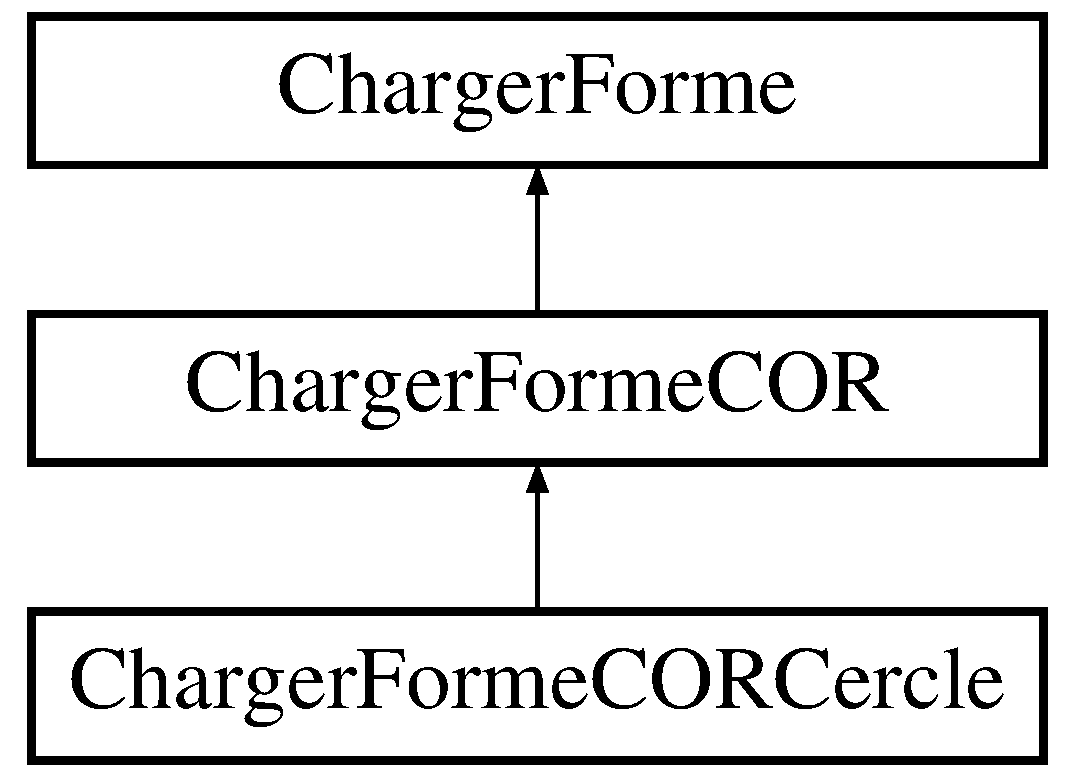
\includegraphics[height=3.000000cm]{class_charger_forme_c_o_r_cercle}
\end{center}
\end{figure}
\subsection*{Public Member Functions}
\begin{DoxyCompactItemize}
\item 
\hyperlink{class_charger_forme_c_o_r_cercle_aa014ab64f0a6c59c9e6d0148ec889e23}{Charger\+Forme\+C\+O\+R\+Cercle} (\hyperlink{class_charger_forme_c_o_r}{Charger\+Forme\+C\+OR} $\ast$suivant)
\begin{DoxyCompactList}\small\item\em Constructeur à partir d\textquotesingle{}un pointeur sur l\textquotesingle{}expert suivant. \end{DoxyCompactList}\item 
const string \hyperlink{class_charger_forme_c_o_r_cercle_a4ca5a036a26641c2636d376f51659172}{get\+Type\+Forme} () const
\begin{DoxyCompactList}\small\item\em Retourne le type de la forme que l\textquotesingle{}expert peut traiter (ici un cercle) \end{DoxyCompactList}\item 
\hyperlink{class_forme}{Forme} $\ast$ \hyperlink{class_charger_forme_c_o_r_cercle_ad65cbf0176ef4a65b44c5782646e45fa}{traiter\+Demande} (const string \&info\+Forme) const
\begin{DoxyCompactList}\small\item\em Extrait les données d\textquotesingle{}une forme à partir d\textquotesingle{}une chaine de caractères. \end{DoxyCompactList}\end{DoxyCompactItemize}
\subsection*{Additional Inherited Members}


\subsection{Constructor \& Destructor Documentation}
\mbox{\Hypertarget{class_charger_forme_c_o_r_cercle_aa014ab64f0a6c59c9e6d0148ec889e23}\label{class_charger_forme_c_o_r_cercle_aa014ab64f0a6c59c9e6d0148ec889e23}} 
\index{Charger\+Forme\+C\+O\+R\+Cercle@{Charger\+Forme\+C\+O\+R\+Cercle}!Charger\+Forme\+C\+O\+R\+Cercle@{Charger\+Forme\+C\+O\+R\+Cercle}}
\index{Charger\+Forme\+C\+O\+R\+Cercle@{Charger\+Forme\+C\+O\+R\+Cercle}!Charger\+Forme\+C\+O\+R\+Cercle@{Charger\+Forme\+C\+O\+R\+Cercle}}
\subsubsection{\texorpdfstring{Charger\+Forme\+C\+O\+R\+Cercle()}{ChargerFormeCORCercle()}}
{\footnotesize\ttfamily Charger\+Forme\+C\+O\+R\+Cercle\+::\+Charger\+Forme\+C\+O\+R\+Cercle (\begin{DoxyParamCaption}\item[{\hyperlink{class_charger_forme_c_o_r}{Charger\+Forme\+C\+OR} $\ast$}]{suivant }\end{DoxyParamCaption})}



Constructeur à partir d\textquotesingle{}un pointeur sur l\textquotesingle{}expert suivant. 


\begin{DoxyParams}{Parameters}
{\em suivant} & Pointeur sur l\textquotesingle{}expert suivant \\
\hline
\end{DoxyParams}


\subsection{Member Function Documentation}
\mbox{\Hypertarget{class_charger_forme_c_o_r_cercle_a4ca5a036a26641c2636d376f51659172}\label{class_charger_forme_c_o_r_cercle_a4ca5a036a26641c2636d376f51659172}} 
\index{Charger\+Forme\+C\+O\+R\+Cercle@{Charger\+Forme\+C\+O\+R\+Cercle}!get\+Type\+Forme@{get\+Type\+Forme}}
\index{get\+Type\+Forme@{get\+Type\+Forme}!Charger\+Forme\+C\+O\+R\+Cercle@{Charger\+Forme\+C\+O\+R\+Cercle}}
\subsubsection{\texorpdfstring{get\+Type\+Forme()}{getTypeForme()}}
{\footnotesize\ttfamily const string Charger\+Forme\+C\+O\+R\+Cercle\+::get\+Type\+Forme (\begin{DoxyParamCaption}{ }\end{DoxyParamCaption}) const\hspace{0.3cm}{\ttfamily [virtual]}}



Retourne le type de la forme que l\textquotesingle{}expert peut traiter (ici un cercle) 

\begin{DoxyReturn}{Returns}
string Type de la forme 
\end{DoxyReturn}


Implements \hyperlink{class_charger_forme_c_o_r_ae740eabcd9b3cc3809c1fe5ffd0100a1}{Charger\+Forme\+C\+OR}.

\mbox{\Hypertarget{class_charger_forme_c_o_r_cercle_ad65cbf0176ef4a65b44c5782646e45fa}\label{class_charger_forme_c_o_r_cercle_ad65cbf0176ef4a65b44c5782646e45fa}} 
\index{Charger\+Forme\+C\+O\+R\+Cercle@{Charger\+Forme\+C\+O\+R\+Cercle}!traiter\+Demande@{traiter\+Demande}}
\index{traiter\+Demande@{traiter\+Demande}!Charger\+Forme\+C\+O\+R\+Cercle@{Charger\+Forme\+C\+O\+R\+Cercle}}
\subsubsection{\texorpdfstring{traiter\+Demande()}{traiterDemande()}}
{\footnotesize\ttfamily \hyperlink{class_forme}{Forme} $\ast$ Charger\+Forme\+C\+O\+R\+Cercle\+::traiter\+Demande (\begin{DoxyParamCaption}\item[{const string \&}]{info\+Forme }\end{DoxyParamCaption}) const\hspace{0.3cm}{\ttfamily [virtual]}}



Extrait les données d\textquotesingle{}une forme à partir d\textquotesingle{}une chaine de caractères. 


\begin{DoxyParams}{Parameters}
{\em info\+Forme} & Chaine de caractères correspondant aux données de la forme \\
\hline
\end{DoxyParams}
\begin{DoxyReturn}{Returns}
Forme$\ast$ Un pointeur sur la forme 
\end{DoxyReturn}


Implements \hyperlink{class_charger_forme_c_o_r_a1d9563c3a1ff9d6d86aa87a83bdaf8da}{Charger\+Forme\+C\+OR}.



The documentation for this class was generated from the following files\+:\begin{DoxyCompactItemize}
\item 
C\+:/\+Users/\+Quentin Fixe/\+Desktop/\+P\+P\+I\+L-\/master/\+C\+L\+I\+E\+N\+T/\hyperlink{_charger_forme_c_o_r_cercle_8h}{Charger\+Forme\+C\+O\+R\+Cercle.\+h}\item 
C\+:/\+Users/\+Quentin Fixe/\+Desktop/\+P\+P\+I\+L-\/master/\+C\+L\+I\+E\+N\+T/\hyperlink{_charger_forme_c_o_r_cercle_8cpp}{Charger\+Forme\+C\+O\+R\+Cercle.\+cpp}\end{DoxyCompactItemize}

\hypertarget{class_charger_forme_c_o_r_groupe}{}\section{Référence de la classe Charger\+Forme\+C\+O\+R\+Groupe}
\label{class_charger_forme_c_o_r_groupe}\index{ChargerFormeCORGroupe@{ChargerFormeCORGroupe}}
Graphe d\textquotesingle{}héritage de Charger\+Forme\+C\+O\+R\+Groupe\+:\begin{figure}[H]
\begin{center}
\leavevmode
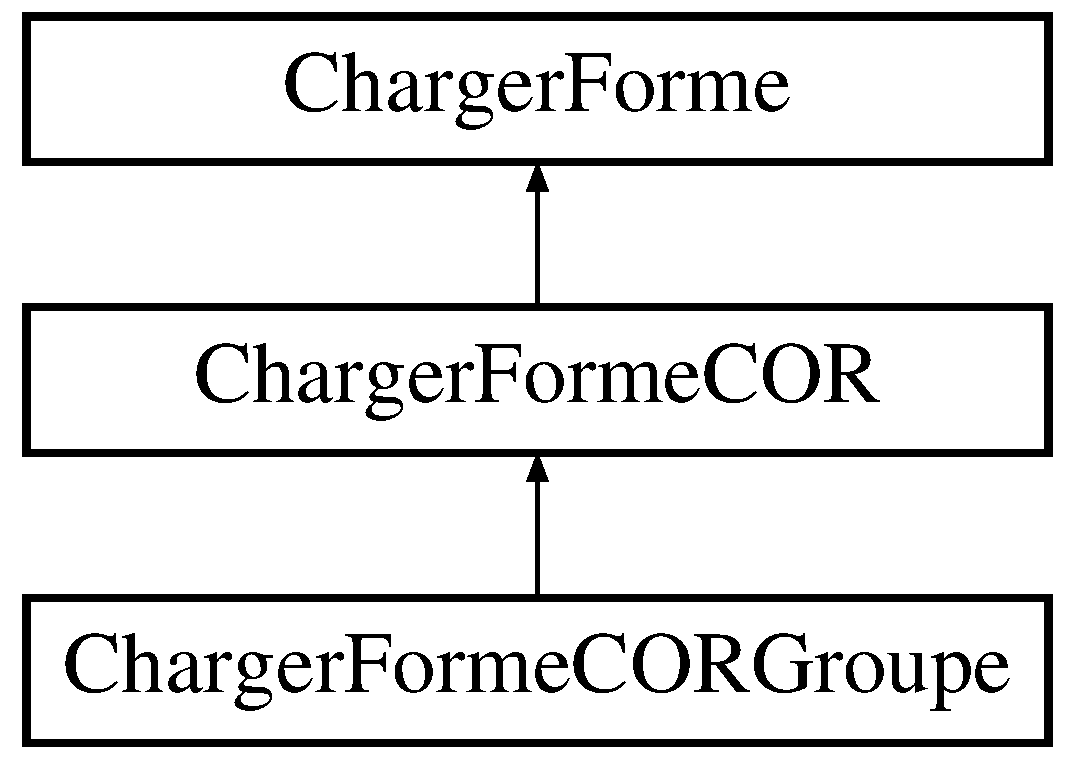
\includegraphics[height=3.000000cm]{class_charger_forme_c_o_r_groupe}
\end{center}
\end{figure}
\subsection*{Fonctions membres publiques}
\begin{DoxyCompactItemize}
\item 
\mbox{\hyperlink{class_charger_forme_c_o_r_groupe_a8af20b68260a8e445aeb0163631f6a66}{Charger\+Forme\+C\+O\+R\+Groupe}} (\mbox{\hyperlink{class_charger_forme_c_o_r}{Charger\+Forme\+C\+OR}} $\ast$suivant)
\begin{DoxyCompactList}\small\item\em Constructeur à partir d\textquotesingle{}un pointeur sur l\textquotesingle{}expert suivant. \end{DoxyCompactList}\item 
const string \mbox{\hyperlink{class_charger_forme_c_o_r_groupe_a202dfd1ec95bc7a20daeb66a92452a11}{get\+Type\+Forme}} () const
\begin{DoxyCompactList}\small\item\em Retourne le type de la forme que l\textquotesingle{}expert peut traiter (ici un groupe) \end{DoxyCompactList}\item 
\mbox{\hyperlink{class_forme}{Forme}} $\ast$ \mbox{\hyperlink{class_charger_forme_c_o_r_groupe_ab28f5a9e7a8fe306c98aa3f1f8b775e4}{traiter\+Demande}} (const string \&info\+Forme) const
\begin{DoxyCompactList}\small\item\em Extrait les données d\textquotesingle{}une forme à partir d\textquotesingle{}une chaine de caractères. \end{DoxyCompactList}\item 
string \mbox{\hyperlink{class_charger_forme_c_o_r_groupe_a6a9f6502bd3d05670a69c8eca418ce06}{get\+Composant}} (string \&copie) const
\begin{DoxyCompactList}\small\item\em Récupère une forme d\textquotesingle{}un groupe. La forme est ensuite supprimée du groupe pour par la suite accéder aux autre formes de ce même groupe. \end{DoxyCompactList}\end{DoxyCompactItemize}
\subsection*{Membres hérités additionnels}


\subsection{Documentation des constructeurs et destructeur}
\mbox{\Hypertarget{class_charger_forme_c_o_r_groupe_a8af20b68260a8e445aeb0163631f6a66}\label{class_charger_forme_c_o_r_groupe_a8af20b68260a8e445aeb0163631f6a66}} 
\index{ChargerFormeCORGroupe@{ChargerFormeCORGroupe}!ChargerFormeCORGroupe@{ChargerFormeCORGroupe}}
\index{ChargerFormeCORGroupe@{ChargerFormeCORGroupe}!ChargerFormeCORGroupe@{ChargerFormeCORGroupe}}
\subsubsection{\texorpdfstring{ChargerFormeCORGroupe()}{ChargerFormeCORGroupe()}}
{\footnotesize\ttfamily Charger\+Forme\+C\+O\+R\+Groupe\+::\+Charger\+Forme\+C\+O\+R\+Groupe (\begin{DoxyParamCaption}\item[{\mbox{\hyperlink{class_charger_forme_c_o_r}{Charger\+Forme\+C\+OR}} $\ast$}]{suivant }\end{DoxyParamCaption})}



Constructeur à partir d\textquotesingle{}un pointeur sur l\textquotesingle{}expert suivant. 


\begin{DoxyParams}{Paramètres}
{\em suivant} & Pointeur sur l\textquotesingle{}expert suivant \\
\hline
\end{DoxyParams}


\subsection{Documentation des fonctions membres}
\mbox{\Hypertarget{class_charger_forme_c_o_r_groupe_a6a9f6502bd3d05670a69c8eca418ce06}\label{class_charger_forme_c_o_r_groupe_a6a9f6502bd3d05670a69c8eca418ce06}} 
\index{ChargerFormeCORGroupe@{ChargerFormeCORGroupe}!getComposant@{getComposant}}
\index{getComposant@{getComposant}!ChargerFormeCORGroupe@{ChargerFormeCORGroupe}}
\subsubsection{\texorpdfstring{getComposant()}{getComposant()}}
{\footnotesize\ttfamily string Charger\+Forme\+C\+O\+R\+Groupe\+::get\+Composant (\begin{DoxyParamCaption}\item[{string \&}]{copie }\end{DoxyParamCaption}) const}



Récupère une forme d\textquotesingle{}un groupe. La forme est ensuite supprimée du groupe pour par la suite accéder aux autre formes de ce même groupe. 


\begin{DoxyParams}{Paramètres}
{\em copier} & Chaine de caractère correspondant au groupe \\
\hline
\end{DoxyParams}
\begin{DoxyReturn}{Renvoie}
string Chaine de caractère correspondant à la forme extraite 
\end{DoxyReturn}
\mbox{\Hypertarget{class_charger_forme_c_o_r_groupe_a202dfd1ec95bc7a20daeb66a92452a11}\label{class_charger_forme_c_o_r_groupe_a202dfd1ec95bc7a20daeb66a92452a11}} 
\index{ChargerFormeCORGroupe@{ChargerFormeCORGroupe}!getTypeForme@{getTypeForme}}
\index{getTypeForme@{getTypeForme}!ChargerFormeCORGroupe@{ChargerFormeCORGroupe}}
\subsubsection{\texorpdfstring{getTypeForme()}{getTypeForme()}}
{\footnotesize\ttfamily const string Charger\+Forme\+C\+O\+R\+Groupe\+::get\+Type\+Forme (\begin{DoxyParamCaption}{ }\end{DoxyParamCaption}) const\hspace{0.3cm}{\ttfamily [virtual]}}



Retourne le type de la forme que l\textquotesingle{}expert peut traiter (ici un groupe) 

\begin{DoxyReturn}{Renvoie}
string Type de la forme 
\end{DoxyReturn}


Implémente \mbox{\hyperlink{class_charger_forme_c_o_r_ae740eabcd9b3cc3809c1fe5ffd0100a1}{Charger\+Forme\+C\+OR}}.

\mbox{\Hypertarget{class_charger_forme_c_o_r_groupe_ab28f5a9e7a8fe306c98aa3f1f8b775e4}\label{class_charger_forme_c_o_r_groupe_ab28f5a9e7a8fe306c98aa3f1f8b775e4}} 
\index{ChargerFormeCORGroupe@{ChargerFormeCORGroupe}!traiterDemande@{traiterDemande}}
\index{traiterDemande@{traiterDemande}!ChargerFormeCORGroupe@{ChargerFormeCORGroupe}}
\subsubsection{\texorpdfstring{traiterDemande()}{traiterDemande()}}
{\footnotesize\ttfamily \mbox{\hyperlink{class_forme}{Forme}} $\ast$ Charger\+Forme\+C\+O\+R\+Groupe\+::traiter\+Demande (\begin{DoxyParamCaption}\item[{const string \&}]{info\+Forme }\end{DoxyParamCaption}) const\hspace{0.3cm}{\ttfamily [virtual]}}



Extrait les données d\textquotesingle{}une forme à partir d\textquotesingle{}une chaine de caractères. 


\begin{DoxyParams}{Paramètres}
{\em info\+Forme} & Chaine de caractères correspondant aux données de la forme \\
\hline
\end{DoxyParams}
\begin{DoxyReturn}{Renvoie}
Forme$\ast$ Un pointeur sur la forme 
\end{DoxyReturn}


Implémente \mbox{\hyperlink{class_charger_forme_c_o_r_a1d9563c3a1ff9d6d86aa87a83bdaf8da}{Charger\+Forme\+C\+OR}}.



La documentation de cette classe a été générée à partir des fichiers suivants \+:\begin{DoxyCompactItemize}
\item 
Charger\+Forme\+C\+O\+R\+Groupe.\+h\item 
Charger\+Forme\+C\+O\+R\+Groupe.\+cpp\end{DoxyCompactItemize}

\hypertarget{class_charger_forme_c_o_r_polygone}{}\section{Charger\+Forme\+C\+O\+R\+Polygone Class Reference}
\label{class_charger_forme_c_o_r_polygone}\index{Charger\+Forme\+C\+O\+R\+Polygone@{Charger\+Forme\+C\+O\+R\+Polygone}}


{\ttfamily \#include $<$Charger\+Forme\+C\+O\+R\+Polygone.\+h$>$}

Inheritance diagram for Charger\+Forme\+C\+O\+R\+Polygone\+:\begin{figure}[H]
\begin{center}
\leavevmode
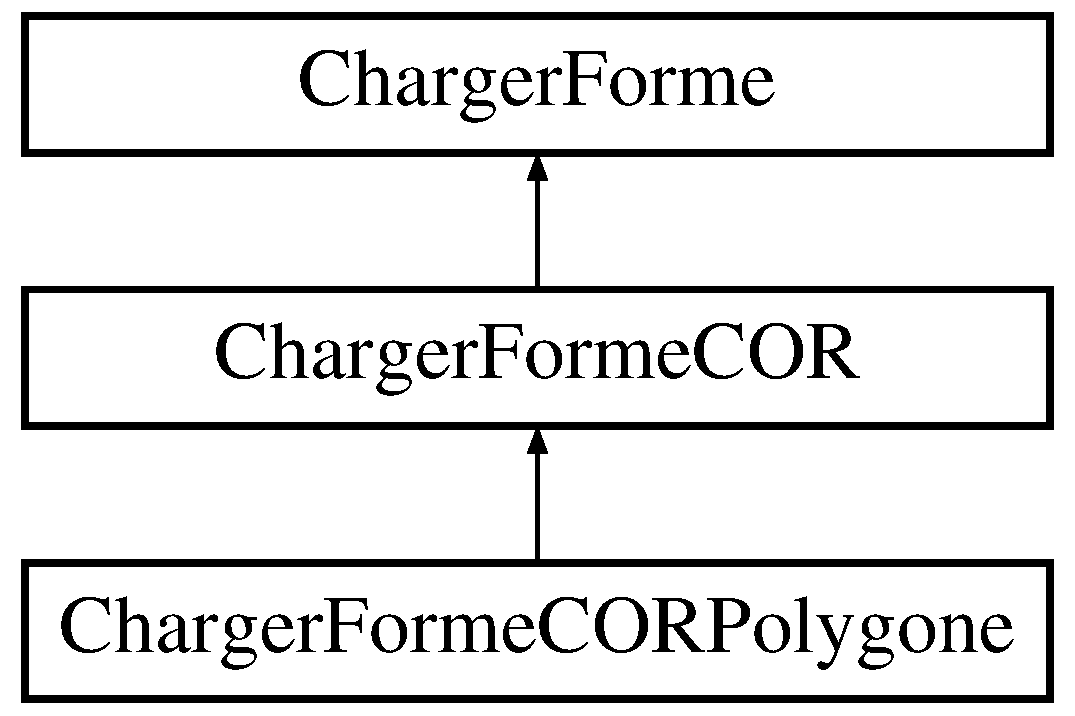
\includegraphics[height=3.000000cm]{class_charger_forme_c_o_r_polygone}
\end{center}
\end{figure}
\subsection*{Public Member Functions}
\begin{DoxyCompactItemize}
\item 
\hyperlink{class_charger_forme_c_o_r_polygone_a177c7353e9c065436dda08540c675b23}{Charger\+Forme\+C\+O\+R\+Polygone} (\hyperlink{class_charger_forme_c_o_r}{Charger\+Forme\+C\+OR} $\ast$suivant)
\begin{DoxyCompactList}\small\item\em Constructeur à partir d\textquotesingle{}un pointeur sur l\textquotesingle{}expert suivant. \end{DoxyCompactList}\item 
const string \hyperlink{class_charger_forme_c_o_r_polygone_a8e702295e28572dc41020965255b847a}{get\+Type\+Forme} () const
\begin{DoxyCompactList}\small\item\em Retourne le type de la forme que l\textquotesingle{}expert peut traiter (ici un polygone) \end{DoxyCompactList}\item 
\hyperlink{class_forme}{Forme} $\ast$ \hyperlink{class_charger_forme_c_o_r_polygone_a4ce89ecdaa400d4930743a8e7204b5f2}{traiter\+Demande} (const string \&info\+Forme) const
\begin{DoxyCompactList}\small\item\em Extrait les données d\textquotesingle{}une forme à partir d\textquotesingle{}une chaine de caractères. \end{DoxyCompactList}\end{DoxyCompactItemize}
\subsection*{Additional Inherited Members}


\subsection{Constructor \& Destructor Documentation}
\mbox{\Hypertarget{class_charger_forme_c_o_r_polygone_a177c7353e9c065436dda08540c675b23}\label{class_charger_forme_c_o_r_polygone_a177c7353e9c065436dda08540c675b23}} 
\index{Charger\+Forme\+C\+O\+R\+Polygone@{Charger\+Forme\+C\+O\+R\+Polygone}!Charger\+Forme\+C\+O\+R\+Polygone@{Charger\+Forme\+C\+O\+R\+Polygone}}
\index{Charger\+Forme\+C\+O\+R\+Polygone@{Charger\+Forme\+C\+O\+R\+Polygone}!Charger\+Forme\+C\+O\+R\+Polygone@{Charger\+Forme\+C\+O\+R\+Polygone}}
\subsubsection{\texorpdfstring{Charger\+Forme\+C\+O\+R\+Polygone()}{ChargerFormeCORPolygone()}}
{\footnotesize\ttfamily Charger\+Forme\+C\+O\+R\+Polygone\+::\+Charger\+Forme\+C\+O\+R\+Polygone (\begin{DoxyParamCaption}\item[{\hyperlink{class_charger_forme_c_o_r}{Charger\+Forme\+C\+OR} $\ast$}]{suivant }\end{DoxyParamCaption})}



Constructeur à partir d\textquotesingle{}un pointeur sur l\textquotesingle{}expert suivant. 


\begin{DoxyParams}{Parameters}
{\em suivant} & Pointeur sur l\textquotesingle{}expert suivant \\
\hline
\end{DoxyParams}


\subsection{Member Function Documentation}
\mbox{\Hypertarget{class_charger_forme_c_o_r_polygone_a8e702295e28572dc41020965255b847a}\label{class_charger_forme_c_o_r_polygone_a8e702295e28572dc41020965255b847a}} 
\index{Charger\+Forme\+C\+O\+R\+Polygone@{Charger\+Forme\+C\+O\+R\+Polygone}!get\+Type\+Forme@{get\+Type\+Forme}}
\index{get\+Type\+Forme@{get\+Type\+Forme}!Charger\+Forme\+C\+O\+R\+Polygone@{Charger\+Forme\+C\+O\+R\+Polygone}}
\subsubsection{\texorpdfstring{get\+Type\+Forme()}{getTypeForme()}}
{\footnotesize\ttfamily const string Charger\+Forme\+C\+O\+R\+Polygone\+::get\+Type\+Forme (\begin{DoxyParamCaption}{ }\end{DoxyParamCaption}) const\hspace{0.3cm}{\ttfamily [virtual]}}



Retourne le type de la forme que l\textquotesingle{}expert peut traiter (ici un polygone) 

\begin{DoxyReturn}{Returns}
string Type de la forme 
\end{DoxyReturn}


Implements \hyperlink{class_charger_forme_c_o_r_ae740eabcd9b3cc3809c1fe5ffd0100a1}{Charger\+Forme\+C\+OR}.

\mbox{\Hypertarget{class_charger_forme_c_o_r_polygone_a4ce89ecdaa400d4930743a8e7204b5f2}\label{class_charger_forme_c_o_r_polygone_a4ce89ecdaa400d4930743a8e7204b5f2}} 
\index{Charger\+Forme\+C\+O\+R\+Polygone@{Charger\+Forme\+C\+O\+R\+Polygone}!traiter\+Demande@{traiter\+Demande}}
\index{traiter\+Demande@{traiter\+Demande}!Charger\+Forme\+C\+O\+R\+Polygone@{Charger\+Forme\+C\+O\+R\+Polygone}}
\subsubsection{\texorpdfstring{traiter\+Demande()}{traiterDemande()}}
{\footnotesize\ttfamily \hyperlink{class_forme}{Forme} $\ast$ Charger\+Forme\+C\+O\+R\+Polygone\+::traiter\+Demande (\begin{DoxyParamCaption}\item[{const string \&}]{info\+Forme }\end{DoxyParamCaption}) const\hspace{0.3cm}{\ttfamily [virtual]}}



Extrait les données d\textquotesingle{}une forme à partir d\textquotesingle{}une chaine de caractères. 


\begin{DoxyParams}{Parameters}
{\em info\+Forme} & Chaine de caractères correspondant aux données de la forme \\
\hline
\end{DoxyParams}
\begin{DoxyReturn}{Returns}
Forme$\ast$ Un pointeur sur la forme 
\end{DoxyReturn}


Implements \hyperlink{class_charger_forme_c_o_r_a1d9563c3a1ff9d6d86aa87a83bdaf8da}{Charger\+Forme\+C\+OR}.



The documentation for this class was generated from the following files\+:\begin{DoxyCompactItemize}
\item 
C\+:/\+Users/\+Quentin Fixe/\+Desktop/\+P\+P\+I\+L-\/master/\+C\+L\+I\+E\+N\+T/\hyperlink{_charger_forme_c_o_r_polygone_8h}{Charger\+Forme\+C\+O\+R\+Polygone.\+h}\item 
C\+:/\+Users/\+Quentin Fixe/\+Desktop/\+P\+P\+I\+L-\/master/\+C\+L\+I\+E\+N\+T/\hyperlink{_charger_forme_c_o_r_polygone_8cpp}{Charger\+Forme\+C\+O\+R\+Polygone.\+cpp}\end{DoxyCompactItemize}

\hypertarget{class_charger_forme_c_o_r_segment}{}\section{Charger\+Forme\+C\+O\+R\+Segment Class Reference}
\label{class_charger_forme_c_o_r_segment}\index{Charger\+Forme\+C\+O\+R\+Segment@{Charger\+Forme\+C\+O\+R\+Segment}}


{\ttfamily \#include $<$Charger\+Forme\+C\+O\+R\+Segment.\+h$>$}

Inheritance diagram for Charger\+Forme\+C\+O\+R\+Segment\+:\begin{figure}[H]
\begin{center}
\leavevmode
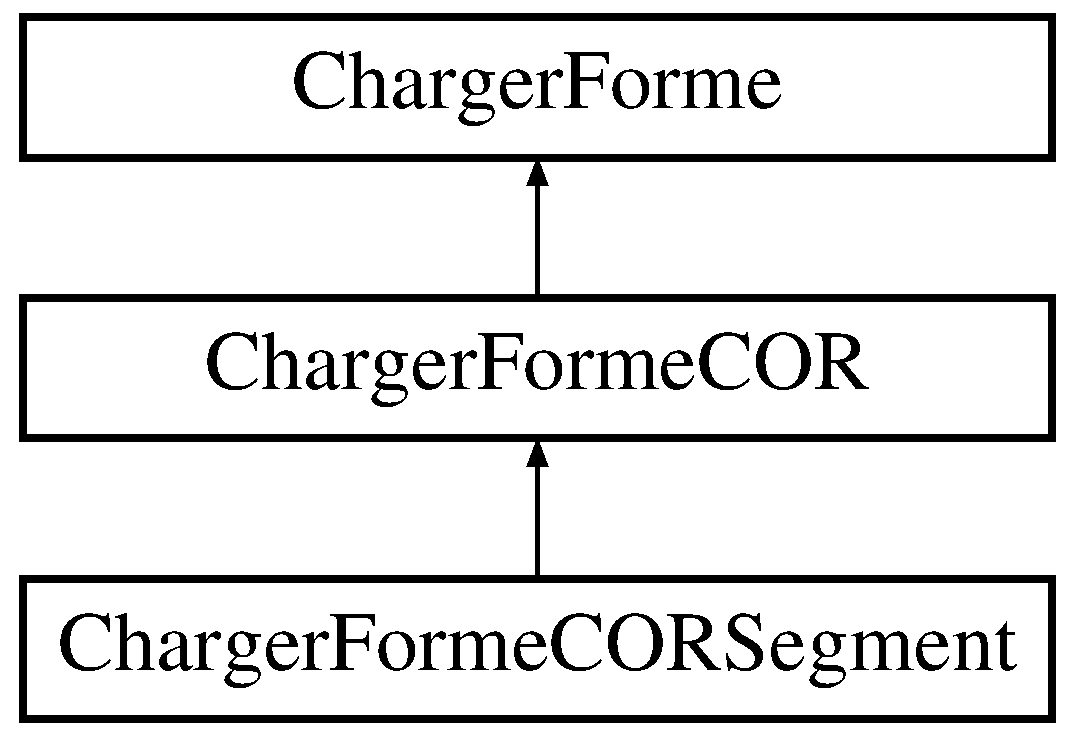
\includegraphics[height=3.000000cm]{class_charger_forme_c_o_r_segment}
\end{center}
\end{figure}
\subsection*{Public Member Functions}
\begin{DoxyCompactItemize}
\item 
\hyperlink{class_charger_forme_c_o_r_segment_ac3a9caaf7fc8e03678cca2161513a1f4}{Charger\+Forme\+C\+O\+R\+Segment} (\hyperlink{class_charger_forme_c_o_r}{Charger\+Forme\+C\+OR} $\ast$suivant)
\begin{DoxyCompactList}\small\item\em Constructeur à partir d\textquotesingle{}un pointeur sur l\textquotesingle{}expert suivant. \end{DoxyCompactList}\item 
const string \hyperlink{class_charger_forme_c_o_r_segment_a88fc3dc3d1e4fb196246f5105965e285}{get\+Type\+Forme} () const
\begin{DoxyCompactList}\small\item\em Retourne le type de la forme que l\textquotesingle{}expert peut traiter (ici un segment) \end{DoxyCompactList}\item 
\hyperlink{class_forme}{Forme} $\ast$ \hyperlink{class_charger_forme_c_o_r_segment_ac7998f4a2669a3f88dc0b204af187780}{traiter\+Demande} (const string \&info\+Forme) const
\begin{DoxyCompactList}\small\item\em Extrait les données d\textquotesingle{}une forme à partir d\textquotesingle{}une chaine de caractères. \end{DoxyCompactList}\end{DoxyCompactItemize}
\subsection*{Additional Inherited Members}


\subsection{Constructor \& Destructor Documentation}
\mbox{\Hypertarget{class_charger_forme_c_o_r_segment_ac3a9caaf7fc8e03678cca2161513a1f4}\label{class_charger_forme_c_o_r_segment_ac3a9caaf7fc8e03678cca2161513a1f4}} 
\index{Charger\+Forme\+C\+O\+R\+Segment@{Charger\+Forme\+C\+O\+R\+Segment}!Charger\+Forme\+C\+O\+R\+Segment@{Charger\+Forme\+C\+O\+R\+Segment}}
\index{Charger\+Forme\+C\+O\+R\+Segment@{Charger\+Forme\+C\+O\+R\+Segment}!Charger\+Forme\+C\+O\+R\+Segment@{Charger\+Forme\+C\+O\+R\+Segment}}
\subsubsection{\texorpdfstring{Charger\+Forme\+C\+O\+R\+Segment()}{ChargerFormeCORSegment()}}
{\footnotesize\ttfamily Charger\+Forme\+C\+O\+R\+Segment\+::\+Charger\+Forme\+C\+O\+R\+Segment (\begin{DoxyParamCaption}\item[{\hyperlink{class_charger_forme_c_o_r}{Charger\+Forme\+C\+OR} $\ast$}]{suivant }\end{DoxyParamCaption})}



Constructeur à partir d\textquotesingle{}un pointeur sur l\textquotesingle{}expert suivant. 


\begin{DoxyParams}{Parameters}
{\em suivant} & Pointeur sur l\textquotesingle{}expert suivant \\
\hline
\end{DoxyParams}


\subsection{Member Function Documentation}
\mbox{\Hypertarget{class_charger_forme_c_o_r_segment_a88fc3dc3d1e4fb196246f5105965e285}\label{class_charger_forme_c_o_r_segment_a88fc3dc3d1e4fb196246f5105965e285}} 
\index{Charger\+Forme\+C\+O\+R\+Segment@{Charger\+Forme\+C\+O\+R\+Segment}!get\+Type\+Forme@{get\+Type\+Forme}}
\index{get\+Type\+Forme@{get\+Type\+Forme}!Charger\+Forme\+C\+O\+R\+Segment@{Charger\+Forme\+C\+O\+R\+Segment}}
\subsubsection{\texorpdfstring{get\+Type\+Forme()}{getTypeForme()}}
{\footnotesize\ttfamily const string Charger\+Forme\+C\+O\+R\+Segment\+::get\+Type\+Forme (\begin{DoxyParamCaption}{ }\end{DoxyParamCaption}) const\hspace{0.3cm}{\ttfamily [virtual]}}



Retourne le type de la forme que l\textquotesingle{}expert peut traiter (ici un segment) 

\begin{DoxyReturn}{Returns}
string Type de la forme 
\end{DoxyReturn}


Implements \hyperlink{class_charger_forme_c_o_r_ae740eabcd9b3cc3809c1fe5ffd0100a1}{Charger\+Forme\+C\+OR}.

\mbox{\Hypertarget{class_charger_forme_c_o_r_segment_ac7998f4a2669a3f88dc0b204af187780}\label{class_charger_forme_c_o_r_segment_ac7998f4a2669a3f88dc0b204af187780}} 
\index{Charger\+Forme\+C\+O\+R\+Segment@{Charger\+Forme\+C\+O\+R\+Segment}!traiter\+Demande@{traiter\+Demande}}
\index{traiter\+Demande@{traiter\+Demande}!Charger\+Forme\+C\+O\+R\+Segment@{Charger\+Forme\+C\+O\+R\+Segment}}
\subsubsection{\texorpdfstring{traiter\+Demande()}{traiterDemande()}}
{\footnotesize\ttfamily \hyperlink{class_forme}{Forme} $\ast$ Charger\+Forme\+C\+O\+R\+Segment\+::traiter\+Demande (\begin{DoxyParamCaption}\item[{const string \&}]{info\+Forme }\end{DoxyParamCaption}) const\hspace{0.3cm}{\ttfamily [virtual]}}



Extrait les données d\textquotesingle{}une forme à partir d\textquotesingle{}une chaine de caractères. 


\begin{DoxyParams}{Parameters}
{\em info\+Forme} & Chaine de caractères correspondant aux données de la forme \\
\hline
\end{DoxyParams}
\begin{DoxyReturn}{Returns}
Forme$\ast$ Un pointeur sur la forme 
\end{DoxyReturn}


Implements \hyperlink{class_charger_forme_c_o_r_a1d9563c3a1ff9d6d86aa87a83bdaf8da}{Charger\+Forme\+C\+OR}.



The documentation for this class was generated from the following files\+:\begin{DoxyCompactItemize}
\item 
C\+:/\+Users/\+Quentin Fixe/\+Desktop/\+P\+P\+I\+L-\/master/\+C\+L\+I\+E\+N\+T/\hyperlink{_charger_forme_c_o_r_segment_8h}{Charger\+Forme\+C\+O\+R\+Segment.\+h}\item 
C\+:/\+Users/\+Quentin Fixe/\+Desktop/\+P\+P\+I\+L-\/master/\+C\+L\+I\+E\+N\+T/\hyperlink{_charger_forme_c_o_r_segment_8cpp}{Charger\+Forme\+C\+O\+R\+Segment.\+cpp}\end{DoxyCompactItemize}

\hypertarget{class_charger_forme_c_o_r_triangle}{}\section{Charger\+Forme\+C\+O\+R\+Triangle Class Reference}
\label{class_charger_forme_c_o_r_triangle}\index{Charger\+Forme\+C\+O\+R\+Triangle@{Charger\+Forme\+C\+O\+R\+Triangle}}


{\ttfamily \#include $<$Charger\+Forme\+C\+O\+R\+Triangle.\+h$>$}

Inheritance diagram for Charger\+Forme\+C\+O\+R\+Triangle\+:\begin{figure}[H]
\begin{center}
\leavevmode
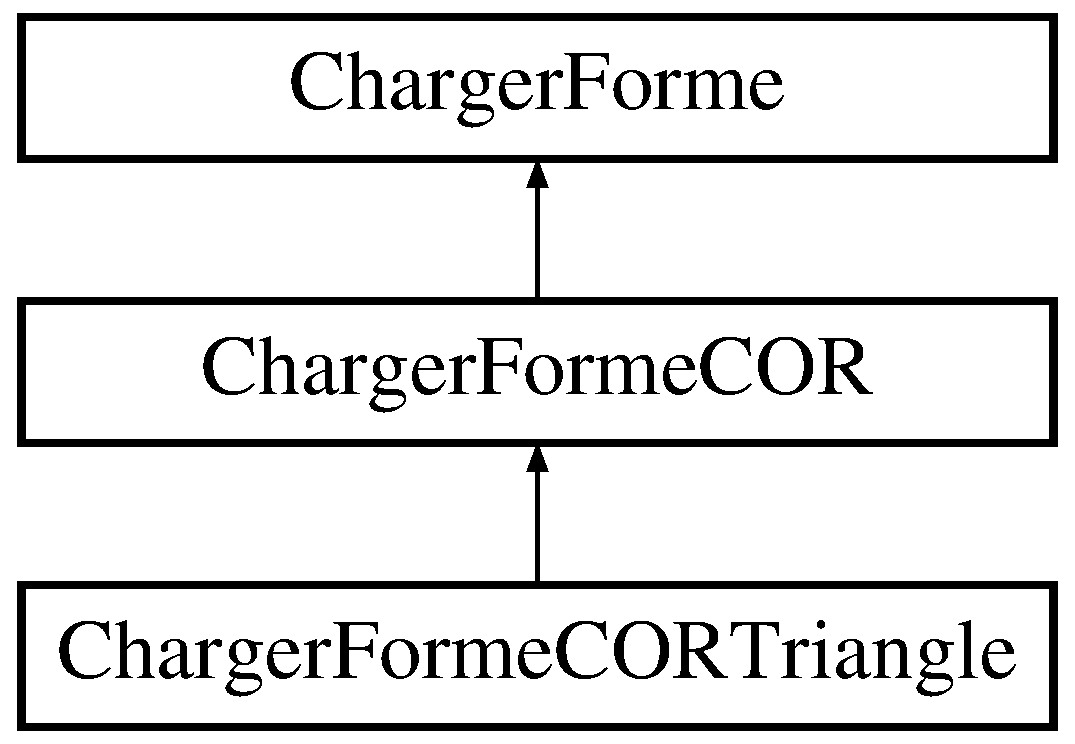
\includegraphics[height=3.000000cm]{class_charger_forme_c_o_r_triangle}
\end{center}
\end{figure}
\subsection*{Public Member Functions}
\begin{DoxyCompactItemize}
\item 
\hyperlink{class_charger_forme_c_o_r_triangle_ab0e825f083ba91bd938d982b5217ca8e}{Charger\+Forme\+C\+O\+R\+Triangle} (\hyperlink{class_charger_forme_c_o_r}{Charger\+Forme\+C\+OR} $\ast$suivant)
\begin{DoxyCompactList}\small\item\em Constructeur à partir d\textquotesingle{}un pointeur sur l\textquotesingle{}expert suivant. \end{DoxyCompactList}\item 
const string \hyperlink{class_charger_forme_c_o_r_triangle_a7a0271b76c6abea8c67be2c920d72925}{get\+Type\+Forme} () const
\begin{DoxyCompactList}\small\item\em Retourne le type de la forme que l\textquotesingle{}expert peut traiter (ici un triangle) \end{DoxyCompactList}\item 
\hyperlink{class_forme}{Forme} $\ast$ \hyperlink{class_charger_forme_c_o_r_triangle_aaa2b1605bb747f29a559f966754237a2}{traiter\+Demande} (const string \&info\+Forme) const
\begin{DoxyCompactList}\small\item\em Extrait les données d\textquotesingle{}une forme à partir d\textquotesingle{}une chaine de caractères. \end{DoxyCompactList}\end{DoxyCompactItemize}
\subsection*{Additional Inherited Members}


\subsection{Constructor \& Destructor Documentation}
\mbox{\Hypertarget{class_charger_forme_c_o_r_triangle_ab0e825f083ba91bd938d982b5217ca8e}\label{class_charger_forme_c_o_r_triangle_ab0e825f083ba91bd938d982b5217ca8e}} 
\index{Charger\+Forme\+C\+O\+R\+Triangle@{Charger\+Forme\+C\+O\+R\+Triangle}!Charger\+Forme\+C\+O\+R\+Triangle@{Charger\+Forme\+C\+O\+R\+Triangle}}
\index{Charger\+Forme\+C\+O\+R\+Triangle@{Charger\+Forme\+C\+O\+R\+Triangle}!Charger\+Forme\+C\+O\+R\+Triangle@{Charger\+Forme\+C\+O\+R\+Triangle}}
\subsubsection{\texorpdfstring{Charger\+Forme\+C\+O\+R\+Triangle()}{ChargerFormeCORTriangle()}}
{\footnotesize\ttfamily Charger\+Forme\+C\+O\+R\+Triangle\+::\+Charger\+Forme\+C\+O\+R\+Triangle (\begin{DoxyParamCaption}\item[{\hyperlink{class_charger_forme_c_o_r}{Charger\+Forme\+C\+OR} $\ast$}]{suivant }\end{DoxyParamCaption})}



Constructeur à partir d\textquotesingle{}un pointeur sur l\textquotesingle{}expert suivant. 


\begin{DoxyParams}{Parameters}
{\em suivant} & Pointeur sur l\textquotesingle{}expert suivant \\
\hline
\end{DoxyParams}


\subsection{Member Function Documentation}
\mbox{\Hypertarget{class_charger_forme_c_o_r_triangle_a7a0271b76c6abea8c67be2c920d72925}\label{class_charger_forme_c_o_r_triangle_a7a0271b76c6abea8c67be2c920d72925}} 
\index{Charger\+Forme\+C\+O\+R\+Triangle@{Charger\+Forme\+C\+O\+R\+Triangle}!get\+Type\+Forme@{get\+Type\+Forme}}
\index{get\+Type\+Forme@{get\+Type\+Forme}!Charger\+Forme\+C\+O\+R\+Triangle@{Charger\+Forme\+C\+O\+R\+Triangle}}
\subsubsection{\texorpdfstring{get\+Type\+Forme()}{getTypeForme()}}
{\footnotesize\ttfamily const string Charger\+Forme\+C\+O\+R\+Triangle\+::get\+Type\+Forme (\begin{DoxyParamCaption}{ }\end{DoxyParamCaption}) const\hspace{0.3cm}{\ttfamily [virtual]}}



Retourne le type de la forme que l\textquotesingle{}expert peut traiter (ici un triangle) 

\begin{DoxyReturn}{Returns}
string Type de la forme 
\end{DoxyReturn}


Implements \hyperlink{class_charger_forme_c_o_r_ae740eabcd9b3cc3809c1fe5ffd0100a1}{Charger\+Forme\+C\+OR}.

\mbox{\Hypertarget{class_charger_forme_c_o_r_triangle_aaa2b1605bb747f29a559f966754237a2}\label{class_charger_forme_c_o_r_triangle_aaa2b1605bb747f29a559f966754237a2}} 
\index{Charger\+Forme\+C\+O\+R\+Triangle@{Charger\+Forme\+C\+O\+R\+Triangle}!traiter\+Demande@{traiter\+Demande}}
\index{traiter\+Demande@{traiter\+Demande}!Charger\+Forme\+C\+O\+R\+Triangle@{Charger\+Forme\+C\+O\+R\+Triangle}}
\subsubsection{\texorpdfstring{traiter\+Demande()}{traiterDemande()}}
{\footnotesize\ttfamily \hyperlink{class_forme}{Forme} $\ast$ Charger\+Forme\+C\+O\+R\+Triangle\+::traiter\+Demande (\begin{DoxyParamCaption}\item[{const string \&}]{info\+Forme }\end{DoxyParamCaption}) const\hspace{0.3cm}{\ttfamily [virtual]}}



Extrait les données d\textquotesingle{}une forme à partir d\textquotesingle{}une chaine de caractères. 


\begin{DoxyParams}{Parameters}
{\em info\+Forme} & Chaine de caractères correspondant aux données de la forme \\
\hline
\end{DoxyParams}
\begin{DoxyReturn}{Returns}
Forme$\ast$ Un pointeur sur la forme 
\end{DoxyReturn}


Implements \hyperlink{class_charger_forme_c_o_r_a1d9563c3a1ff9d6d86aa87a83bdaf8da}{Charger\+Forme\+C\+OR}.



The documentation for this class was generated from the following files\+:\begin{DoxyCompactItemize}
\item 
C\+:/\+Users/\+Quentin Fixe/\+Desktop/\+P\+P\+I\+L-\/master/\+C\+L\+I\+E\+N\+T/\hyperlink{_charger_forme_c_o_r_triangle_8h}{Charger\+Forme\+C\+O\+R\+Triangle.\+h}\item 
C\+:/\+Users/\+Quentin Fixe/\+Desktop/\+P\+P\+I\+L-\/master/\+C\+L\+I\+E\+N\+T/\hyperlink{_charger_forme_c_o_r_triangle_8cpp}{Charger\+Forme\+C\+O\+R\+Triangle.\+cpp}\end{DoxyCompactItemize}

\hypertarget{class_c_o_r}{}\section{C\+OR Class Reference}
\label{class_c_o_r}\index{C\+OR@{C\+OR}}


{\ttfamily \#include $<$C\+O\+R.\+h$>$}

\subsection*{Public Member Functions}
\begin{DoxyCompactItemize}
\item 
\hyperlink{class_charger_forme}{Charger\+Forme} $\ast$ \hyperlink{class_c_o_r_a868c62e34fa6f203f4f09b3d354b8226}{get\+Chargeur\+Forme} ()
\begin{DoxyCompactList}\small\item\em m�thode pour r�cup�rer le chargeur forme. \end{DoxyCompactList}\end{DoxyCompactItemize}
\subsection*{Static Public Member Functions}
\begin{DoxyCompactItemize}
\item 
static \hyperlink{class_c_o_r}{C\+OR} $\ast$ \hyperlink{class_c_o_r_af85f8dfa9ca05cb1c93b0398a398eec7}{get\+Instance} ()
\begin{DoxyCompactList}\small\item\em m�thode pour r�cup�rer l\textquotesingle{}instance de la classe. \end{DoxyCompactList}\end{DoxyCompactItemize}


\subsection{Member Function Documentation}
\mbox{\Hypertarget{class_c_o_r_a868c62e34fa6f203f4f09b3d354b8226}\label{class_c_o_r_a868c62e34fa6f203f4f09b3d354b8226}} 
\index{C\+OR@{C\+OR}!get\+Chargeur\+Forme@{get\+Chargeur\+Forme}}
\index{get\+Chargeur\+Forme@{get\+Chargeur\+Forme}!C\+OR@{C\+OR}}
\subsubsection{\texorpdfstring{get\+Chargeur\+Forme()}{getChargeurForme()}}
{\footnotesize\ttfamily \hyperlink{class_charger_forme}{Charger\+Forme} $\ast$ C\+O\+R\+::get\+Chargeur\+Forme (\begin{DoxyParamCaption}{ }\end{DoxyParamCaption})}



m�thode pour r�cup�rer le chargeur forme. 

\begin{DoxyReturn}{Returns}
\hyperlink{class_c_o_r}{C\+OR} $\ast$ l\textquotesingle{}instance. 
\end{DoxyReturn}
\mbox{\Hypertarget{class_c_o_r_af85f8dfa9ca05cb1c93b0398a398eec7}\label{class_c_o_r_af85f8dfa9ca05cb1c93b0398a398eec7}} 
\index{C\+OR@{C\+OR}!get\+Instance@{get\+Instance}}
\index{get\+Instance@{get\+Instance}!C\+OR@{C\+OR}}
\subsubsection{\texorpdfstring{get\+Instance()}{getInstance()}}
{\footnotesize\ttfamily \hyperlink{class_c_o_r}{C\+OR} $\ast$ C\+O\+R\+::get\+Instance (\begin{DoxyParamCaption}{ }\end{DoxyParamCaption})\hspace{0.3cm}{\ttfamily [static]}}



m�thode pour r�cup�rer l\textquotesingle{}instance de la classe. 

\begin{DoxyReturn}{Returns}
\hyperlink{class_c_o_r}{C\+OR} $\ast$ l\textquotesingle{}instance. 
\end{DoxyReturn}


The documentation for this class was generated from the following files\+:\begin{DoxyCompactItemize}
\item 
C\+:/\+Users/\+Quentin Fixe/\+Desktop/\+P\+P\+I\+L-\/master/\+C\+L\+I\+E\+N\+T/\hyperlink{_c_o_r_8h}{C\+O\+R.\+h}\item 
C\+:/\+Users/\+Quentin Fixe/\+Desktop/\+P\+P\+I\+L-\/master/\+C\+L\+I\+E\+N\+T/\hyperlink{_c_o_r_8cpp}{C\+O\+R.\+cpp}\end{DoxyCompactItemize}

\hypertarget{class_couleur}{}\section{Référence de la classe Couleur}
\label{class_couleur}\index{Couleur@{Couleur}}
\subsection*{Fonctions membres publiques}
\begin{DoxyCompactItemize}
\item 
\mbox{\Hypertarget{class_couleur_a687a457edb08b51dbcd0299bb0b6a882}\label{class_couleur_a687a457edb08b51dbcd0299bb0b6a882}} 
\mbox{\hyperlink{class_couleur_a687a457edb08b51dbcd0299bb0b6a882}{Couleur}} ()
\begin{DoxyCompactList}\small\item\em Constructeur par défaut d\textquotesingle{}une couleur. \end{DoxyCompactList}\item 
\mbox{\hyperlink{class_couleur_a3875e178605e5a425a473b9034f796b3}{Couleur}} (const string \&nom\+Couleur)
\begin{DoxyCompactList}\small\item\em Constructeur à partir d\textquotesingle{}une chaine de caractères. \end{DoxyCompactList}\item 
\mbox{\hyperlink{class_couleur_ae5694f3994756524981394433bbdc85f}{Couleur}} (const \mbox{\hyperlink{class_couleur}{Couleur}} \&couleur)
\begin{DoxyCompactList}\small\item\em Constructeur à partir d\textquotesingle{}une couleur. \end{DoxyCompactList}\item 
\mbox{\Hypertarget{class_couleur_ad3be30be83649bc5db48ef46b592aec2}\label{class_couleur_ad3be30be83649bc5db48ef46b592aec2}} 
virtual \mbox{\hyperlink{class_couleur_ad3be30be83649bc5db48ef46b592aec2}{$\sim$\+Couleur}} ()
\begin{DoxyCompactList}\small\item\em Destructeur. \end{DoxyCompactList}\item 
bool \mbox{\hyperlink{class_couleur_ab426fe44e27a92cf0faf8fee1e086a5f}{contains}} (string nom\+Couleur)
\begin{DoxyCompactList}\small\item\em Teste si une couleur existe. \end{DoxyCompactList}\item 
const string \& \mbox{\hyperlink{class_couleur_a0e38cc8477e1618b317124ab372c3501}{get\+Nom\+Couleur}} () const
\begin{DoxyCompactList}\small\item\em Getter pour récupérer la couleur. \end{DoxyCompactList}\item 
void \mbox{\hyperlink{class_couleur_a571f1d6faacd4ee99f0180400ccb259d}{set\+Nom\+Couleur}} (const string \&nom\+Couleur)
\begin{DoxyCompactList}\small\item\em Setter pour modifier la couleur. \end{DoxyCompactList}\item 
\mbox{\hyperlink{class_couleur_acff55563e5760e4cea32ca275eb62205}{operator string}} () const
\begin{DoxyCompactList}\small\item\em Surcharge de l\textquotesingle{}opérateur pour convertir une couleur en string. \end{DoxyCompactList}\item 
bool \mbox{\hyperlink{class_couleur_a159c6c550e8855d6a44765ab5e0b0de8}{operator==}} (const \mbox{\hyperlink{class_couleur}{Couleur}} \&objet) const
\begin{DoxyCompactList}\small\item\em Surcharge de l\textquotesingle{}opérateur == pour comparer deux couleurs. \end{DoxyCompactList}\item 
bool \mbox{\hyperlink{class_couleur_ade329eaaf3db16de47b3be59b3c13198}{operator !=}} (const \mbox{\hyperlink{class_couleur}{Couleur}} \&objet) const
\begin{DoxyCompactList}\small\item\em Surcharge de l\textquotesingle{}opérateur != pour comparer deux couleurs, on utilise ==. \end{DoxyCompactList}\item 
const \mbox{\hyperlink{class_couleur}{Couleur}} \mbox{\hyperlink{class_couleur_af49bf608ba98af5f9dfe19fbe2759000}{operator=}} (const \mbox{\hyperlink{class_couleur}{Couleur}} \&couleur)
\begin{DoxyCompactList}\small\item\em Surcharge de l\textquotesingle{}opérateur = pour affecter les valeurs d\textquotesingle{}une couleur à une autre. \end{DoxyCompactList}\end{DoxyCompactItemize}
\subsection*{Amis}
\begin{DoxyCompactItemize}
\item 
ostream \& \mbox{\hyperlink{class_couleur_a8223b4eee2017fdd318d16692a16c636}{operator$<$$<$}} (ostream \&flux, const \mbox{\hyperlink{class_couleur}{Couleur}} \&coul)
\begin{DoxyCompactList}\small\item\em Surcharge de l\textquotesingle{}opérateur $<$$<$ pour l\textquotesingle{}affichage des couleurs. \end{DoxyCompactList}\end{DoxyCompactItemize}


\subsection{Documentation des constructeurs et destructeur}
\mbox{\Hypertarget{class_couleur_a3875e178605e5a425a473b9034f796b3}\label{class_couleur_a3875e178605e5a425a473b9034f796b3}} 
\index{Couleur@{Couleur}!Couleur@{Couleur}}
\index{Couleur@{Couleur}!Couleur@{Couleur}}
\subsubsection{\texorpdfstring{Couleur()}{Couleur()}\hspace{0.1cm}{\footnotesize\ttfamily [1/2]}}
{\footnotesize\ttfamily Couleur\+::\+Couleur (\begin{DoxyParamCaption}\item[{const string \&}]{nom\+Couleur }\end{DoxyParamCaption})}



Constructeur à partir d\textquotesingle{}une chaine de caractères. 


\begin{DoxyParams}{Paramètres}
{\em couleur} & Une chaine de caractère représentant la couleur \\
\hline
\end{DoxyParams}
\mbox{\Hypertarget{class_couleur_ae5694f3994756524981394433bbdc85f}\label{class_couleur_ae5694f3994756524981394433bbdc85f}} 
\index{Couleur@{Couleur}!Couleur@{Couleur}}
\index{Couleur@{Couleur}!Couleur@{Couleur}}
\subsubsection{\texorpdfstring{Couleur()}{Couleur()}\hspace{0.1cm}{\footnotesize\ttfamily [2/2]}}
{\footnotesize\ttfamily Couleur\+::\+Couleur (\begin{DoxyParamCaption}\item[{const \mbox{\hyperlink{class_couleur}{Couleur}} \&}]{couleur }\end{DoxyParamCaption})}



Constructeur à partir d\textquotesingle{}une couleur. 


\begin{DoxyParams}{Paramètres}
{\em couleur} & Une couleur \\
\hline
\end{DoxyParams}


\subsection{Documentation des fonctions membres}
\mbox{\Hypertarget{class_couleur_ab426fe44e27a92cf0faf8fee1e086a5f}\label{class_couleur_ab426fe44e27a92cf0faf8fee1e086a5f}} 
\index{Couleur@{Couleur}!contains@{contains}}
\index{contains@{contains}!Couleur@{Couleur}}
\subsubsection{\texorpdfstring{contains()}{contains()}}
{\footnotesize\ttfamily bool Couleur\+::contains (\begin{DoxyParamCaption}\item[{string}]{nom\+Couleur }\end{DoxyParamCaption})}



Teste si une couleur existe. 


\begin{DoxyParams}{Paramètres}
{\em bool} & Renvoie vrai si la couleur existe, faux sinon \\
\hline
\end{DoxyParams}
\mbox{\Hypertarget{class_couleur_a0e38cc8477e1618b317124ab372c3501}\label{class_couleur_a0e38cc8477e1618b317124ab372c3501}} 
\index{Couleur@{Couleur}!getNomCouleur@{getNomCouleur}}
\index{getNomCouleur@{getNomCouleur}!Couleur@{Couleur}}
\subsubsection{\texorpdfstring{getNomCouleur()}{getNomCouleur()}}
{\footnotesize\ttfamily const string \& Couleur\+::get\+Nom\+Couleur (\begin{DoxyParamCaption}{ }\end{DoxyParamCaption}) const}



Getter pour récupérer la couleur. 

\begin{DoxyReturn}{Renvoie}
string Une chaine de caractère correspondant à la couleur 
\end{DoxyReturn}
\mbox{\Hypertarget{class_couleur_ade329eaaf3db16de47b3be59b3c13198}\label{class_couleur_ade329eaaf3db16de47b3be59b3c13198}} 
\index{Couleur@{Couleur}!operator "!=@{operator "!=}}
\index{operator "!=@{operator "!=}!Couleur@{Couleur}}
\subsubsection{\texorpdfstring{operator "!=()}{operator !=()}}
{\footnotesize\ttfamily bool Couleur\+::operator != (\begin{DoxyParamCaption}\item[{const \mbox{\hyperlink{class_couleur}{Couleur}} \&}]{objet }\end{DoxyParamCaption}) const}



Surcharge de l\textquotesingle{}opérateur != pour comparer deux couleurs, on utilise ==. 


\begin{DoxyParams}{Paramètres}
{\em objet} & La couleur à comparer \\
\hline
{\em y} & Réel \\
\hline
\end{DoxyParams}
\mbox{\Hypertarget{class_couleur_acff55563e5760e4cea32ca275eb62205}\label{class_couleur_acff55563e5760e4cea32ca275eb62205}} 
\index{Couleur@{Couleur}!operator string@{operator string}}
\index{operator string@{operator string}!Couleur@{Couleur}}
\subsubsection{\texorpdfstring{operator string()}{operator string()}}
{\footnotesize\ttfamily Couleur\+::operator string (\begin{DoxyParamCaption}{ }\end{DoxyParamCaption}) const}



Surcharge de l\textquotesingle{}opérateur pour convertir une couleur en string. 

C\+Onversion d\textquotesingle{}une couleur en chaine de caractères \mbox{\Hypertarget{class_couleur_af49bf608ba98af5f9dfe19fbe2759000}\label{class_couleur_af49bf608ba98af5f9dfe19fbe2759000}} 
\index{Couleur@{Couleur}!operator=@{operator=}}
\index{operator=@{operator=}!Couleur@{Couleur}}
\subsubsection{\texorpdfstring{operator=()}{operator=()}}
{\footnotesize\ttfamily const \mbox{\hyperlink{class_couleur}{Couleur}} Couleur\+::operator= (\begin{DoxyParamCaption}\item[{const \mbox{\hyperlink{class_couleur}{Couleur}} \&}]{couleur }\end{DoxyParamCaption})}



Surcharge de l\textquotesingle{}opérateur = pour affecter les valeurs d\textquotesingle{}une couleur à une autre. 


\begin{DoxyParams}{Paramètres}
{\em couleur} & La couleur à affecter \\
\hline
\end{DoxyParams}
\begin{DoxyReturn}{Renvoie}
Coulur Objet constant de la couleur qui a été affectée 
\end{DoxyReturn}
\mbox{\Hypertarget{class_couleur_a159c6c550e8855d6a44765ab5e0b0de8}\label{class_couleur_a159c6c550e8855d6a44765ab5e0b0de8}} 
\index{Couleur@{Couleur}!operator==@{operator==}}
\index{operator==@{operator==}!Couleur@{Couleur}}
\subsubsection{\texorpdfstring{operator==()}{operator==()}}
{\footnotesize\ttfamily bool Couleur\+::operator== (\begin{DoxyParamCaption}\item[{const \mbox{\hyperlink{class_couleur}{Couleur}} \&}]{objet }\end{DoxyParamCaption}) const}



Surcharge de l\textquotesingle{}opérateur == pour comparer deux couleurs. 


\begin{DoxyParams}{Paramètres}
{\em objet} & La couleur à comparer \\
\hline
\end{DoxyParams}
\begin{DoxyReturn}{Renvoie}
bool Un booléen vrai si les deux couleurs dont identiques, faux sinon 
\end{DoxyReturn}
\mbox{\Hypertarget{class_couleur_a571f1d6faacd4ee99f0180400ccb259d}\label{class_couleur_a571f1d6faacd4ee99f0180400ccb259d}} 
\index{Couleur@{Couleur}!setNomCouleur@{setNomCouleur}}
\index{setNomCouleur@{setNomCouleur}!Couleur@{Couleur}}
\subsubsection{\texorpdfstring{setNomCouleur()}{setNomCouleur()}}
{\footnotesize\ttfamily void Couleur\+::set\+Nom\+Couleur (\begin{DoxyParamCaption}\item[{const string \&}]{nom\+Couleur }\end{DoxyParamCaption})}



Setter pour modifier la couleur. 


\begin{DoxyParams}{Paramètres}
{\em couleur} & Une chaine de caractère correspondant à la couleur à modifier \\
\hline
\end{DoxyParams}


\subsection{Documentation des fonctions amies et associées}
\mbox{\Hypertarget{class_couleur_a8223b4eee2017fdd318d16692a16c636}\label{class_couleur_a8223b4eee2017fdd318d16692a16c636}} 
\index{Couleur@{Couleur}!operator$<$$<$@{operator$<$$<$}}
\index{operator$<$$<$@{operator$<$$<$}!Couleur@{Couleur}}
\subsubsection{\texorpdfstring{operator$<$$<$}{operator<<}}
{\footnotesize\ttfamily ostream\& operator$<$$<$ (\begin{DoxyParamCaption}\item[{ostream \&}]{flux,  }\item[{const \mbox{\hyperlink{class_couleur}{Couleur}} \&}]{coul }\end{DoxyParamCaption})\hspace{0.3cm}{\ttfamily [friend]}}



Surcharge de l\textquotesingle{}opérateur $<$$<$ pour l\textquotesingle{}affichage des couleurs. 


\begin{DoxyParams}{Paramètres}
{\em flux} & Le flux de sortie \\
\hline
{\em coul} & La couleur à afficher \\
\hline
\end{DoxyParams}
\begin{DoxyReturn}{Renvoie}
ostream Le flux de sortie 
\end{DoxyReturn}


La documentation de cette classe a été générée à partir des fichiers suivants \+:\begin{DoxyCompactItemize}
\item 
\mbox{\hyperlink{_couleur_8h}{Couleur.\+h}}\item 
Couleur.\+cpp\end{DoxyCompactItemize}

\hypertarget{class_exception}{}\section{Exception Class Reference}
\label{class_exception}\index{Exception@{Exception}}


{\ttfamily \#include $<$Exception.\+h$>$}

\subsection*{Public Member Functions}
\begin{DoxyCompactItemize}
\item 
\hyperlink{class_exception_a2936fbe9591faf7418fb8b6b0be8c9be}{Exception} (const string \&msg)
\begin{DoxyCompactList}\small\item\em Seul constructeur de la classe \hyperlink{class_exception}{Exception}. \end{DoxyCompactList}\item 
const string \& \hyperlink{class_exception_a4e6ab5d6ff666b6d71a9b886a8af6e61}{get\+Message} () const
\begin{DoxyCompactList}\small\item\em Getter de l\textquotesingle{}attribut priv� m\+\_\+msg. \end{DoxyCompactList}\end{DoxyCompactItemize}
\subsection*{Friends}
\begin{DoxyCompactItemize}
\item 
ostream \& \hyperlink{class_exception_a88684adfbd9ebf35e8145ab1b1216621}{operator$<$$<$} (ostream \&flux, const \hyperlink{class_exception}{Exception} \&e)
\end{DoxyCompactItemize}


\subsection{Constructor \& Destructor Documentation}
\mbox{\Hypertarget{class_exception_a2936fbe9591faf7418fb8b6b0be8c9be}\label{class_exception_a2936fbe9591faf7418fb8b6b0be8c9be}} 
\index{Exception@{Exception}!Exception@{Exception}}
\index{Exception@{Exception}!Exception@{Exception}}
\subsubsection{\texorpdfstring{Exception()}{Exception()}}
{\footnotesize\ttfamily Exception\+::\+Exception (\begin{DoxyParamCaption}\item[{const string \&}]{msg }\end{DoxyParamCaption})\hspace{0.3cm}{\ttfamily [inline]}}



Seul constructeur de la classe \hyperlink{class_exception}{Exception}. 

message d\textquotesingle{}exception 
\begin{DoxyParams}{Parameters}
{\em string} & msg \\
\hline
\end{DoxyParams}


\subsection{Member Function Documentation}
\mbox{\Hypertarget{class_exception_a4e6ab5d6ff666b6d71a9b886a8af6e61}\label{class_exception_a4e6ab5d6ff666b6d71a9b886a8af6e61}} 
\index{Exception@{Exception}!get\+Message@{get\+Message}}
\index{get\+Message@{get\+Message}!Exception@{Exception}}
\subsubsection{\texorpdfstring{get\+Message()}{getMessage()}}
{\footnotesize\ttfamily const string\& Exception\+::get\+Message (\begin{DoxyParamCaption}{ }\end{DoxyParamCaption}) const\hspace{0.3cm}{\ttfamily [inline]}}



Getter de l\textquotesingle{}attribut priv� m\+\_\+msg. 

\begin{DoxyReturn}{Returns}
string Ce que contient l\textquotesingle{}attribut priv� m\+\_\+msg 
\end{DoxyReturn}


\subsection{Friends And Related Function Documentation}
\mbox{\Hypertarget{class_exception_a88684adfbd9ebf35e8145ab1b1216621}\label{class_exception_a88684adfbd9ebf35e8145ab1b1216621}} 
\index{Exception@{Exception}!operator$<$$<$@{operator$<$$<$}}
\index{operator$<$$<$@{operator$<$$<$}!Exception@{Exception}}
\subsubsection{\texorpdfstring{operator$<$$<$}{operator<<}}
{\footnotesize\ttfamily ostream\& operator$<$$<$ (\begin{DoxyParamCaption}\item[{ostream \&}]{flux,  }\item[{const \hyperlink{class_exception}{Exception} \&}]{e }\end{DoxyParamCaption})\hspace{0.3cm}{\ttfamily [friend]}}

\textbackslash{} brief Surcharge l\textquotesingle{}affichage dans un flux. 
\begin{DoxyParams}{Parameters}
{\em flux} & Flux sortant \\
\hline
{\em e} & \hyperlink{class_exception}{Exception} \\
\hline
\end{DoxyParams}
\begin{DoxyReturn}{Returns}
ostream Flux sortant 
\end{DoxyReturn}


The documentation for this class was generated from the following file\+:\begin{DoxyCompactItemize}
\item 
C\+:/\+Users/\+Quentin Fixe/\+Desktop/\+P\+P\+I\+L-\/master/\+C\+L\+I\+E\+N\+T/\hyperlink{_exception_8h}{Exception.\+h}\end{DoxyCompactItemize}

\hypertarget{class_forme}{}\section{Forme Class Reference}
\label{class_forme}\index{Forme@{Forme}}


{\ttfamily \#include $<$Forme.\+h$>$}

Inheritance diagram for Forme\+:\begin{figure}[H]
\begin{center}
\leavevmode
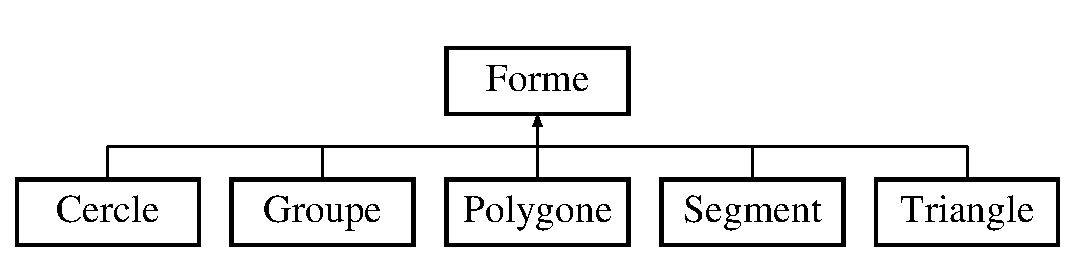
\includegraphics[height=2.000000cm]{class_forme}
\end{center}
\end{figure}
\subsection*{Public Member Functions}
\begin{DoxyCompactItemize}
\item 
\hyperlink{class_forme_a3c97c1066856b548d2fe6db963a28800}{Forme} ()
\begin{DoxyCompactList}\small\item\em Constructeur par d�faut de \hyperlink{class_forme}{Forme}. \end{DoxyCompactList}\item 
\hyperlink{class_forme_aa82486cc0a585afad8d1af1c24146572}{Forme} (const \hyperlink{class_couleur}{Couleur} \&couleur)
\begin{DoxyCompactList}\small\item\em Constructeur � partir d\textquotesingle{}une couleur. \end{DoxyCompactList}\item 
\hyperlink{class_forme_a92f5316091ea6d77881b5b648e26d47a}{Forme} (const \hyperlink{class_forme}{Forme} $\ast$forme)
\begin{DoxyCompactList}\small\item\em Constructeur de recopie � partir d\textquotesingle{}un pointeur de \hyperlink{class_forme}{Forme}. \end{DoxyCompactList}\item 
virtual \hyperlink{class_forme_af6ad0735f86713459453c9d775f44aca}{$\sim$\+Forme} ()
\begin{DoxyCompactList}\small\item\em Destructeur virtual qui sera appel� pour tous les h�ritiers de \hyperlink{class_forme}{Forme}. \end{DoxyCompactList}\item 
const \hyperlink{class_couleur}{Couleur} \& \hyperlink{class_forme_a2797ab2fc6b73d78eed90b8f289d8ae2}{get\+Couleur} () const
\begin{DoxyCompactList}\small\item\em Getter pour r�cup�rer la couleur d\textquotesingle{}une forme. \end{DoxyCompactList}\item 
virtual void \hyperlink{class_forme_a7669632f8153916c4feeb845cc4676dc}{set\+Couleur} (const \hyperlink{class_couleur}{Couleur} \&couleur)
\begin{DoxyCompactList}\small\item\em Setter pour modifier la couleur de la forme. \end{DoxyCompactList}\item 
bool \hyperlink{class_forme_af7566f80f907102025e669b9c4d8ceba}{est\+Marquee} () const
\begin{DoxyCompactList}\small\item\em Getter pour savoir si une forme fait parti d\textquotesingle{}un groupe. \end{DoxyCompactList}\item 
void \hyperlink{class_forme_a471001d1511460f157d5a7813846b534}{set\+Marquee} (bool marquee)
\begin{DoxyCompactList}\small\item\em Setter qui permet de marquer une forme si elle fait parti d\textquotesingle{}un groupe. \end{DoxyCompactList}\item 
virtual \hyperlink{class_forme_a809375f023f0f19227f3e3821ee56731}{operator string} () const
\begin{DoxyCompactList}\small\item\em Surcharge de l\textquotesingle{}op�rateur string permettant de convertir des formes en string. \end{DoxyCompactList}\item 
virtual bool \hyperlink{class_forme_a7a9608681318db43231fd7e7872af8ab}{operator==} (const \hyperlink{class_forme}{Forme} \&objet) const
\begin{DoxyCompactList}\small\item\em Surcharge de l\textquotesingle{}op�rateur == qui teste si deux formes sont identiques. \end{DoxyCompactList}\item 
virtual bool \hyperlink{class_forme_ae7f1157657d766ee2da54fc73bb74d15}{operator!=} (const \hyperlink{class_forme}{Forme} \&objet) const
\begin{DoxyCompactList}\small\item\em Surcharge de l\textquotesingle{}op�rateur != qui utilise ==. \end{DoxyCompactList}\item 
virtual const \hyperlink{class_forme}{Forme} $\ast$ \hyperlink{class_forme_a7c9d26b86d294e68126e748ca8b093f0}{operator=} (const \hyperlink{class_forme}{Forme} \&forme)
\begin{DoxyCompactList}\small\item\em Surcharge de l\textquotesingle{}op�rateur = qui permet d\textquotesingle{}affcter une forme � une autre. \end{DoxyCompactList}\item 
virtual const double \hyperlink{class_forme_adf4346150d8f734d7a48f7661e30cab4}{get\+Aire} () const =0
\begin{DoxyCompactList}\small\item\em Getter recup�re l\textquotesingle{}aire de la forme propre � chaque forme (m�thode virtuelle pure) \end{DoxyCompactList}\item 
virtual \hyperlink{class_forme}{Forme} $\ast$ \hyperlink{class_forme_a226750dc3f772514fe58e1dc16f3d0d5}{clone} () const =0
\begin{DoxyCompactList}\small\item\em Clone une forme (m�thode virtuelle pure) \end{DoxyCompactList}\item 
virtual void \hyperlink{class_forme_aeaae98ea3de8523de9ba9093e19779d8}{homothetie} (const \hyperlink{class_vecteur2_d}{Vecteur2D} \&vect\+Homotethie, double k)=0
\begin{DoxyCompactList}\small\item\em Effectue une homot�thie sur la forme (M�thode vitruelle pure) \end{DoxyCompactList}\item 
virtual void \hyperlink{class_forme_ad156a02098ef453b09919b2a3156f607}{translation} (const \hyperlink{class_vecteur2_d}{Vecteur2D} \&vect\+Translation)=0
\begin{DoxyCompactList}\small\item\em Effectue une translation sur la forme (M�thode virtuelle pure) \end{DoxyCompactList}\item 
virtual void \hyperlink{class_forme_af17c4156d00281b4b62d8c27dcb75569}{rotation} (const \hyperlink{class_vecteur2_d}{Vecteur2D} \&vect\+Centre, double angle)=0
\begin{DoxyCompactList}\small\item\em Effectue une rotation sur la forme. \end{DoxyCompactList}\item 
virtual ostream \& \hyperlink{class_forme_a348a12ae03fe2167ffd586f4deae6c76}{print} (ostream \&flux) const
\begin{DoxyCompactList}\small\item\em M�thode permettant d\textquotesingle{}afficher les informations concernant la forme. \end{DoxyCompactList}\item 
virtual void \hyperlink{class_forme_a7be10bca98001dc368adc3a3e93d0f48}{accepte\+Sauvegarder} (const \hyperlink{class_visiteur_sauv_t_x_t}{Visiteur\+Sauv\+T\+XT} $\ast$v) const =0
\begin{DoxyCompactList}\small\item\em Appelle la m�thode visite du visiteur de sauvegarde correpondant � la forme. \end{DoxyCompactList}\item 
virtual void \hyperlink{class_forme_a8cd4879a6a5751cbf6d3bbbfbec41566}{dessiner} (const \hyperlink{class_visiteur_dessin}{Visiteur\+Dessin} $\ast$v) const =0
\begin{DoxyCompactList}\small\item\em Appelle la m�thode visite du visiteur de dessin correpondant � la forme. \end{DoxyCompactList}\end{DoxyCompactItemize}
\subsection*{Friends}
\begin{DoxyCompactItemize}
\item 
ostream \& \hyperlink{class_forme_ab34818bedc1e61133319fa46f3d10f0b}{operator$<$$<$} (ostream \&flux, const \hyperlink{class_forme}{Forme} \&forme)
\begin{DoxyCompactList}\small\item\em Surcharge de l\textquotesingle{}op�rateur $<$$<$ pour l\textquotesingle{}affichage d\textquotesingle{}une forme. \end{DoxyCompactList}\end{DoxyCompactItemize}


\subsection{Constructor \& Destructor Documentation}
\mbox{\Hypertarget{class_forme_a3c97c1066856b548d2fe6db963a28800}\label{class_forme_a3c97c1066856b548d2fe6db963a28800}} 
\index{Forme@{Forme}!Forme@{Forme}}
\index{Forme@{Forme}!Forme@{Forme}}
\subsubsection{\texorpdfstring{Forme()}{Forme()}\hspace{0.1cm}{\footnotesize\ttfamily [1/3]}}
{\footnotesize\ttfamily Forme\+::\+Forme (\begin{DoxyParamCaption}{ }\end{DoxyParamCaption})}



Constructeur par d�faut de \hyperlink{class_forme}{Forme}. 

\mbox{\Hypertarget{class_forme_aa82486cc0a585afad8d1af1c24146572}\label{class_forme_aa82486cc0a585afad8d1af1c24146572}} 
\index{Forme@{Forme}!Forme@{Forme}}
\index{Forme@{Forme}!Forme@{Forme}}
\subsubsection{\texorpdfstring{Forme()}{Forme()}\hspace{0.1cm}{\footnotesize\ttfamily [2/3]}}
{\footnotesize\ttfamily Forme\+::\+Forme (\begin{DoxyParamCaption}\item[{const \hyperlink{class_couleur}{Couleur} \&}]{couleur }\end{DoxyParamCaption})}



Constructeur � partir d\textquotesingle{}une couleur. 


\begin{DoxyParams}{Parameters}
{\em couleur} & Une couleur � appliquer � la forme \\
\hline
\end{DoxyParams}
\mbox{\Hypertarget{class_forme_a92f5316091ea6d77881b5b648e26d47a}\label{class_forme_a92f5316091ea6d77881b5b648e26d47a}} 
\index{Forme@{Forme}!Forme@{Forme}}
\index{Forme@{Forme}!Forme@{Forme}}
\subsubsection{\texorpdfstring{Forme()}{Forme()}\hspace{0.1cm}{\footnotesize\ttfamily [3/3]}}
{\footnotesize\ttfamily Forme\+::\+Forme (\begin{DoxyParamCaption}\item[{const \hyperlink{class_forme}{Forme} $\ast$}]{forme }\end{DoxyParamCaption})}



Constructeur de recopie � partir d\textquotesingle{}un pointeur de \hyperlink{class_forme}{Forme}. 

Les coordonn�es x et y sont par d�faut mis � 0. 
\begin{DoxyParams}{Parameters}
{\em x} & R�el \\
\hline
{\em y} & R�el \\
\hline
\end{DoxyParams}
\mbox{\Hypertarget{class_forme_af6ad0735f86713459453c9d775f44aca}\label{class_forme_af6ad0735f86713459453c9d775f44aca}} 
\index{Forme@{Forme}!````~Forme@{$\sim$\+Forme}}
\index{````~Forme@{$\sim$\+Forme}!Forme@{Forme}}
\subsubsection{\texorpdfstring{$\sim$\+Forme()}{~Forme()}}
{\footnotesize\ttfamily Forme\+::$\sim$\+Forme (\begin{DoxyParamCaption}{ }\end{DoxyParamCaption})\hspace{0.3cm}{\ttfamily [virtual]}}



Destructeur virtual qui sera appel� pour tous les h�ritiers de \hyperlink{class_forme}{Forme}. 



\subsection{Member Function Documentation}
\mbox{\Hypertarget{class_forme_a7be10bca98001dc368adc3a3e93d0f48}\label{class_forme_a7be10bca98001dc368adc3a3e93d0f48}} 
\index{Forme@{Forme}!accepte\+Sauvegarder@{accepte\+Sauvegarder}}
\index{accepte\+Sauvegarder@{accepte\+Sauvegarder}!Forme@{Forme}}
\subsubsection{\texorpdfstring{accepte\+Sauvegarder()}{accepteSauvegarder()}}
{\footnotesize\ttfamily virtual void Forme\+::accepte\+Sauvegarder (\begin{DoxyParamCaption}\item[{const \hyperlink{class_visiteur_sauv_t_x_t}{Visiteur\+Sauv\+T\+XT} $\ast$}]{v }\end{DoxyParamCaption}) const\hspace{0.3cm}{\ttfamily [pure virtual]}}



Appelle la m�thode visite du visiteur de sauvegarde correpondant � la forme. 


\begin{DoxyParams}{Parameters}
{\em v} & Pointeur sur le visiteur de sauvegarde \\
\hline
\end{DoxyParams}


Implemented in \hyperlink{class_triangle_af0ad5baa5cd45c0a1afd40690ebed849}{Triangle}, \hyperlink{class_polygone_af97fb141e2b4b0042c8f0998b0499af3}{Polygone}, \hyperlink{class_cercle_a681df3cd077879881755a727b950a263}{Cercle}, \hyperlink{class_groupe_a69ab923874f5eb9ff4e0dc8dd4d359e5}{Groupe}, and \hyperlink{class_segment_aaad6697e62e1e881ef6aa21a91b6d9ca}{Segment}.

\mbox{\Hypertarget{class_forme_a226750dc3f772514fe58e1dc16f3d0d5}\label{class_forme_a226750dc3f772514fe58e1dc16f3d0d5}} 
\index{Forme@{Forme}!clone@{clone}}
\index{clone@{clone}!Forme@{Forme}}
\subsubsection{\texorpdfstring{clone()}{clone()}}
{\footnotesize\ttfamily virtual \hyperlink{class_forme}{Forme}$\ast$ Forme\+::clone (\begin{DoxyParamCaption}{ }\end{DoxyParamCaption}) const\hspace{0.3cm}{\ttfamily [pure virtual]}}



Clone une forme (m�thode virtuelle pure) 

\begin{DoxyReturn}{Returns}
Forme$\ast$ Un pointeur sur l\textquotesingle{}objet clon� 
\end{DoxyReturn}


Implemented in \hyperlink{class_triangle_a610a6de862fd2f720036ae515dd71930}{Triangle}, \hyperlink{class_polygone_a3efc2ac3ad92c3609f6d5f8fe9039871}{Polygone}, \hyperlink{class_cercle_a56073052a84c4b8e04124692e6dc58f5}{Cercle}, \hyperlink{class_groupe_a614513db9e80b6e6c0811da16d89bb19}{Groupe}, and \hyperlink{class_segment_a219b06579e425a818933813df8b22232}{Segment}.

\mbox{\Hypertarget{class_forme_a8cd4879a6a5751cbf6d3bbbfbec41566}\label{class_forme_a8cd4879a6a5751cbf6d3bbbfbec41566}} 
\index{Forme@{Forme}!dessiner@{dessiner}}
\index{dessiner@{dessiner}!Forme@{Forme}}
\subsubsection{\texorpdfstring{dessiner()}{dessiner()}}
{\footnotesize\ttfamily virtual void Forme\+::dessiner (\begin{DoxyParamCaption}\item[{const \hyperlink{class_visiteur_dessin}{Visiteur\+Dessin} $\ast$}]{v }\end{DoxyParamCaption}) const\hspace{0.3cm}{\ttfamily [pure virtual]}}



Appelle la m�thode visite du visiteur de dessin correpondant � la forme. 


\begin{DoxyParams}{Parameters}
{\em v} & Pointeur sur le visiteur de dessin \\
\hline
\end{DoxyParams}


Implemented in \hyperlink{class_triangle_af4d344ab356b33b90a095022adc42434}{Triangle}, \hyperlink{class_polygone_a2e71a18fa658499da019558913e7ccbb}{Polygone}, \hyperlink{class_cercle_a2d3d99149647f033b6f8f470c9a1f53f}{Cercle}, \hyperlink{class_groupe_ae62001512056945a4233c168977e9a1c}{Groupe}, and \hyperlink{class_segment_a11de1e065225eb89e7b952a51e918276}{Segment}.

\mbox{\Hypertarget{class_forme_af7566f80f907102025e669b9c4d8ceba}\label{class_forme_af7566f80f907102025e669b9c4d8ceba}} 
\index{Forme@{Forme}!est\+Marquee@{est\+Marquee}}
\index{est\+Marquee@{est\+Marquee}!Forme@{Forme}}
\subsubsection{\texorpdfstring{est\+Marquee()}{estMarquee()}}
{\footnotesize\ttfamily bool Forme\+::est\+Marquee (\begin{DoxyParamCaption}{ }\end{DoxyParamCaption}) const}



Getter pour savoir si une forme fait parti d\textquotesingle{}un groupe. 

\begin{DoxyReturn}{Returns}
bool un bool�en vrai si la forme est dans un groupe, faux sinon 
\end{DoxyReturn}
\mbox{\Hypertarget{class_forme_adf4346150d8f734d7a48f7661e30cab4}\label{class_forme_adf4346150d8f734d7a48f7661e30cab4}} 
\index{Forme@{Forme}!get\+Aire@{get\+Aire}}
\index{get\+Aire@{get\+Aire}!Forme@{Forme}}
\subsubsection{\texorpdfstring{get\+Aire()}{getAire()}}
{\footnotesize\ttfamily virtual const double Forme\+::get\+Aire (\begin{DoxyParamCaption}{ }\end{DoxyParamCaption}) const\hspace{0.3cm}{\ttfamily [pure virtual]}}



Getter recup�re l\textquotesingle{}aire de la forme propre � chaque forme (m�thode virtuelle pure) 

\begin{DoxyReturn}{Returns}
L\textquotesingle{}aire de la forme 
\end{DoxyReturn}


Implemented in \hyperlink{class_triangle_aa6693ea9778fad637f7b1c73a305c220}{Triangle}, \hyperlink{class_polygone_a07880a169f0241140d15cdbca13a3622}{Polygone}, \hyperlink{class_groupe_afc0056987479b35eedafa6cc5b758288}{Groupe}, \hyperlink{class_cercle_a2477495263095a5553f2bcfa524f03ac}{Cercle}, and \hyperlink{class_segment_ab5d7a7584c28a3f306ce9f82b9b71d43}{Segment}.

\mbox{\Hypertarget{class_forme_a2797ab2fc6b73d78eed90b8f289d8ae2}\label{class_forme_a2797ab2fc6b73d78eed90b8f289d8ae2}} 
\index{Forme@{Forme}!get\+Couleur@{get\+Couleur}}
\index{get\+Couleur@{get\+Couleur}!Forme@{Forme}}
\subsubsection{\texorpdfstring{get\+Couleur()}{getCouleur()}}
{\footnotesize\ttfamily const \hyperlink{class_couleur}{Couleur} \& Forme\+::get\+Couleur (\begin{DoxyParamCaption}{ }\end{DoxyParamCaption}) const}



Getter pour r�cup�rer la couleur d\textquotesingle{}une forme. 

\begin{DoxyReturn}{Returns}
\hyperlink{class_couleur}{Couleur} La couleur de la forme 
\end{DoxyReturn}
\mbox{\Hypertarget{class_forme_aeaae98ea3de8523de9ba9093e19779d8}\label{class_forme_aeaae98ea3de8523de9ba9093e19779d8}} 
\index{Forme@{Forme}!homothetie@{homothetie}}
\index{homothetie@{homothetie}!Forme@{Forme}}
\subsubsection{\texorpdfstring{homothetie()}{homothetie()}}
{\footnotesize\ttfamily virtual void Forme\+::homothetie (\begin{DoxyParamCaption}\item[{const \hyperlink{class_vecteur2_d}{Vecteur2D} \&}]{vect\+Homotethie,  }\item[{double}]{k }\end{DoxyParamCaption})\hspace{0.3cm}{\ttfamily [pure virtual]}}



Effectue une homot�thie sur la forme (M�thode vitruelle pure) 


\begin{DoxyParams}{Parameters}
{\em vect\+Homotethie} & \hyperlink{class_vecteur2_d}{Vecteur2D} \\
\hline
{\em k} & R�el \\
\hline
\end{DoxyParams}


Implemented in \hyperlink{class_triangle_a2c15a4513cf35c9275b237ec70bf6df2}{Triangle}, \hyperlink{class_polygone_a211ccacc83e547e0b7cd129e23e8cf1d}{Polygone}, \hyperlink{class_cercle_a41c2ecef959a6273a08d44806351f0f4}{Cercle}, \hyperlink{class_groupe_a597ef92844df8aeb27f0a47a9b3f9209}{Groupe}, and \hyperlink{class_segment_aa71198ab2350e4536a9bdbb0f8179a05}{Segment}.

\mbox{\Hypertarget{class_forme_a809375f023f0f19227f3e3821ee56731}\label{class_forme_a809375f023f0f19227f3e3821ee56731}} 
\index{Forme@{Forme}!operator string@{operator string}}
\index{operator string@{operator string}!Forme@{Forme}}
\subsubsection{\texorpdfstring{operator string()}{operator string()}}
{\footnotesize\ttfamily Forme\+::operator string (\begin{DoxyParamCaption}{ }\end{DoxyParamCaption}) const\hspace{0.3cm}{\ttfamily [virtual]}}



Surcharge de l\textquotesingle{}op�rateur string permettant de convertir des formes en string. 



Reimplemented in \hyperlink{class_triangle_acd8612cc20ffb71e543944c869e4ab81}{Triangle}, \hyperlink{class_cercle_a01dfce2b49afb0dcb5bd176d4145b71a}{Cercle}, \hyperlink{class_segment_a28b3be893a35a0d73574354752c147fd}{Segment}, \hyperlink{class_polygone_abd801a84b5306df8021f1571d82deafd}{Polygone}, and \hyperlink{class_groupe_ab8bcab328da985da9907cffe76ca71d0}{Groupe}.

\mbox{\Hypertarget{class_forme_ae7f1157657d766ee2da54fc73bb74d15}\label{class_forme_ae7f1157657d766ee2da54fc73bb74d15}} 
\index{Forme@{Forme}!operator"!=@{operator"!=}}
\index{operator"!=@{operator"!=}!Forme@{Forme}}
\subsubsection{\texorpdfstring{operator"!=()}{operator!=()}}
{\footnotesize\ttfamily bool Forme\+::operator!= (\begin{DoxyParamCaption}\item[{const \hyperlink{class_forme}{Forme} \&}]{objet }\end{DoxyParamCaption}) const\hspace{0.3cm}{\ttfamily [virtual]}}



Surcharge de l\textquotesingle{}op�rateur != qui utilise ==. 

Teste si deux formes sont diff�rentes 
\begin{DoxyParams}{Parameters}
{\em objet} & La forme � comparer \\
\hline
\end{DoxyParams}
\begin{DoxyReturn}{Returns}
bool Un bool�en vrai si les deux formes sont diff�rentes, faux sinon 
\end{DoxyReturn}
\mbox{\Hypertarget{class_forme_a7c9d26b86d294e68126e748ca8b093f0}\label{class_forme_a7c9d26b86d294e68126e748ca8b093f0}} 
\index{Forme@{Forme}!operator=@{operator=}}
\index{operator=@{operator=}!Forme@{Forme}}
\subsubsection{\texorpdfstring{operator=()}{operator=()}}
{\footnotesize\ttfamily const \hyperlink{class_forme}{Forme} $\ast$ Forme\+::operator= (\begin{DoxyParamCaption}\item[{const \hyperlink{class_forme}{Forme} \&}]{forme }\end{DoxyParamCaption})\hspace{0.3cm}{\ttfamily [virtual]}}



Surcharge de l\textquotesingle{}op�rateur = qui permet d\textquotesingle{}affcter une forme � une autre. 


\begin{DoxyParams}{Parameters}
{\em forme} & La forme � affecter \\
\hline
\end{DoxyParams}
\begin{DoxyReturn}{Returns}
Forme$\ast$ Un pointeur sur \hyperlink{class_forme}{Forme} 
\end{DoxyReturn}
\mbox{\Hypertarget{class_forme_a7a9608681318db43231fd7e7872af8ab}\label{class_forme_a7a9608681318db43231fd7e7872af8ab}} 
\index{Forme@{Forme}!operator==@{operator==}}
\index{operator==@{operator==}!Forme@{Forme}}
\subsubsection{\texorpdfstring{operator==()}{operator==()}}
{\footnotesize\ttfamily bool Forme\+::operator== (\begin{DoxyParamCaption}\item[{const \hyperlink{class_forme}{Forme} \&}]{objet }\end{DoxyParamCaption}) const\hspace{0.3cm}{\ttfamily [virtual]}}



Surcharge de l\textquotesingle{}op�rateur == qui teste si deux formes sont identiques. 


\begin{DoxyParams}{Parameters}
{\em objet} & La forme � comparer \\
\hline
\end{DoxyParams}
\begin{DoxyReturn}{Returns}
bool Un bool�en vrai si les deux formes sont identiques, faux sinon 
\end{DoxyReturn}
\mbox{\Hypertarget{class_forme_a348a12ae03fe2167ffd586f4deae6c76}\label{class_forme_a348a12ae03fe2167ffd586f4deae6c76}} 
\index{Forme@{Forme}!print@{print}}
\index{print@{print}!Forme@{Forme}}
\subsubsection{\texorpdfstring{print()}{print()}}
{\footnotesize\ttfamily ostream \& Forme\+::print (\begin{DoxyParamCaption}\item[{ostream \&}]{flux }\end{DoxyParamCaption}) const\hspace{0.3cm}{\ttfamily [virtual]}}



M�thode permettant d\textquotesingle{}afficher les informations concernant la forme. 


\begin{DoxyParams}{Parameters}
{\em flux} & Flux de sortie \\
\hline
\end{DoxyParams}
\begin{DoxyReturn}{Returns}
ostream Flux de sortie 
\end{DoxyReturn}


Reimplemented in \hyperlink{class_triangle_a9e810bfe4577a2e590235d5388cbee03}{Triangle}, \hyperlink{class_polygone_a3c8534deace725beaaaa0657ad720822}{Polygone}, \hyperlink{class_cercle_a80410c399a44cfa15bd2fd19df8f3648}{Cercle}, \hyperlink{class_groupe_a83b86a306fae5bd4dfb4461d44b5e343}{Groupe}, and \hyperlink{class_segment_a41e90e3615ca17a67ac0fe0bb3a99223}{Segment}.

\mbox{\Hypertarget{class_forme_af17c4156d00281b4b62d8c27dcb75569}\label{class_forme_af17c4156d00281b4b62d8c27dcb75569}} 
\index{Forme@{Forme}!rotation@{rotation}}
\index{rotation@{rotation}!Forme@{Forme}}
\subsubsection{\texorpdfstring{rotation()}{rotation()}}
{\footnotesize\ttfamily virtual void Forme\+::rotation (\begin{DoxyParamCaption}\item[{const \hyperlink{class_vecteur2_d}{Vecteur2D} \&}]{vect\+Centre,  }\item[{double}]{angle }\end{DoxyParamCaption})\hspace{0.3cm}{\ttfamily [pure virtual]}}



Effectue une rotation sur la forme. 


\begin{DoxyParams}{Parameters}
{\em vect\+Centre} & \hyperlink{class_vecteur2_d}{Vecteur2D} \\
\hline
{\em angle} & R�el \\
\hline
\end{DoxyParams}


Implemented in \hyperlink{class_triangle_a6e728d1e72366e42b2afbf1e13b6d8f7}{Triangle}, \hyperlink{class_polygone_a5f30d9d61cfc6c3f2cafd345f8fc8824}{Polygone}, \hyperlink{class_cercle_a6cabe637a245d902e5bfe7d82efd493f}{Cercle}, \hyperlink{class_groupe_a4bdf9f82744057cff6706a2889c2ec68}{Groupe}, and \hyperlink{class_segment_a77c334ce9c358ff3dc72b431b380eabe}{Segment}.

\mbox{\Hypertarget{class_forme_a7669632f8153916c4feeb845cc4676dc}\label{class_forme_a7669632f8153916c4feeb845cc4676dc}} 
\index{Forme@{Forme}!set\+Couleur@{set\+Couleur}}
\index{set\+Couleur@{set\+Couleur}!Forme@{Forme}}
\subsubsection{\texorpdfstring{set\+Couleur()}{setCouleur()}}
{\footnotesize\ttfamily void Forme\+::set\+Couleur (\begin{DoxyParamCaption}\item[{const \hyperlink{class_couleur}{Couleur} \&}]{couleur }\end{DoxyParamCaption})\hspace{0.3cm}{\ttfamily [virtual]}}



Setter pour modifier la couleur de la forme. 


\begin{DoxyParams}{Parameters}
{\em couleur} & Chaine de caract�re correspondant � la couleur \\
\hline
\end{DoxyParams}
\mbox{\Hypertarget{class_forme_a471001d1511460f157d5a7813846b534}\label{class_forme_a471001d1511460f157d5a7813846b534}} 
\index{Forme@{Forme}!set\+Marquee@{set\+Marquee}}
\index{set\+Marquee@{set\+Marquee}!Forme@{Forme}}
\subsubsection{\texorpdfstring{set\+Marquee()}{setMarquee()}}
{\footnotesize\ttfamily void Forme\+::set\+Marquee (\begin{DoxyParamCaption}\item[{bool}]{marquee }\end{DoxyParamCaption})}



Setter qui permet de marquer une forme si elle fait parti d\textquotesingle{}un groupe. 


\begin{DoxyParams}{Parameters}
{\em marquee} & Marquer la forme par vrai ou faux \\
\hline
\end{DoxyParams}
\mbox{\Hypertarget{class_forme_ad156a02098ef453b09919b2a3156f607}\label{class_forme_ad156a02098ef453b09919b2a3156f607}} 
\index{Forme@{Forme}!translation@{translation}}
\index{translation@{translation}!Forme@{Forme}}
\subsubsection{\texorpdfstring{translation()}{translation()}}
{\footnotesize\ttfamily virtual void Forme\+::translation (\begin{DoxyParamCaption}\item[{const \hyperlink{class_vecteur2_d}{Vecteur2D} \&}]{vect\+Translation }\end{DoxyParamCaption})\hspace{0.3cm}{\ttfamily [pure virtual]}}



Effectue une translation sur la forme (M�thode virtuelle pure) 


\begin{DoxyParams}{Parameters}
{\em vect\+Translation} & \hyperlink{class_vecteur2_d}{Vecteur2D} \\
\hline
\end{DoxyParams}


Implemented in \hyperlink{class_triangle_aa1b2a542395e4e8c67f35757159c4d4b}{Triangle}, \hyperlink{class_polygone_a4c4e05250d5ebebbb3d544011be0dbd7}{Polygone}, \hyperlink{class_cercle_aec369809aab0faf3adc93c62e6acc06c}{Cercle}, \hyperlink{class_groupe_a0cbd34b8d5f3d29cae4acbebd07e5af2}{Groupe}, and \hyperlink{class_segment_acd838b6258da2a18d1f0f5f76d32b6d1}{Segment}.



\subsection{Friends And Related Function Documentation}
\mbox{\Hypertarget{class_forme_ab34818bedc1e61133319fa46f3d10f0b}\label{class_forme_ab34818bedc1e61133319fa46f3d10f0b}} 
\index{Forme@{Forme}!operator$<$$<$@{operator$<$$<$}}
\index{operator$<$$<$@{operator$<$$<$}!Forme@{Forme}}
\subsubsection{\texorpdfstring{operator$<$$<$}{operator<<}}
{\footnotesize\ttfamily ostream\& operator$<$$<$ (\begin{DoxyParamCaption}\item[{ostream \&}]{flux,  }\item[{const \hyperlink{class_forme}{Forme} \&}]{forme }\end{DoxyParamCaption})\hspace{0.3cm}{\ttfamily [friend]}}



Surcharge de l\textquotesingle{}op�rateur $<$$<$ pour l\textquotesingle{}affichage d\textquotesingle{}une forme. 


\begin{DoxyParams}{Parameters}
{\em flux} & Flux de sortie \\
\hline
{\em forme} & La forme � afficher \\
\hline
\end{DoxyParams}
\begin{DoxyReturn}{Returns}
ostream Flux de sortie 
\end{DoxyReturn}


The documentation for this class was generated from the following files\+:\begin{DoxyCompactItemize}
\item 
C\+:/\+Users/\+Quentin Fixe/\+Desktop/\+P\+P\+I\+L-\/master/\+C\+L\+I\+E\+N\+T/\hyperlink{_forme_8h}{Forme.\+h}\item 
C\+:/\+Users/\+Quentin Fixe/\+Desktop/\+P\+P\+I\+L-\/master/\+C\+L\+I\+E\+N\+T/\hyperlink{_forme_8cpp}{Forme.\+cpp}\end{DoxyCompactItemize}

\hypertarget{class_groupe}{}\section{Référence de la classe Groupe}
\label{class_groupe}\index{Groupe@{Groupe}}
Graphe d\textquotesingle{}héritage de Groupe\+:\begin{figure}[H]
\begin{center}
\leavevmode
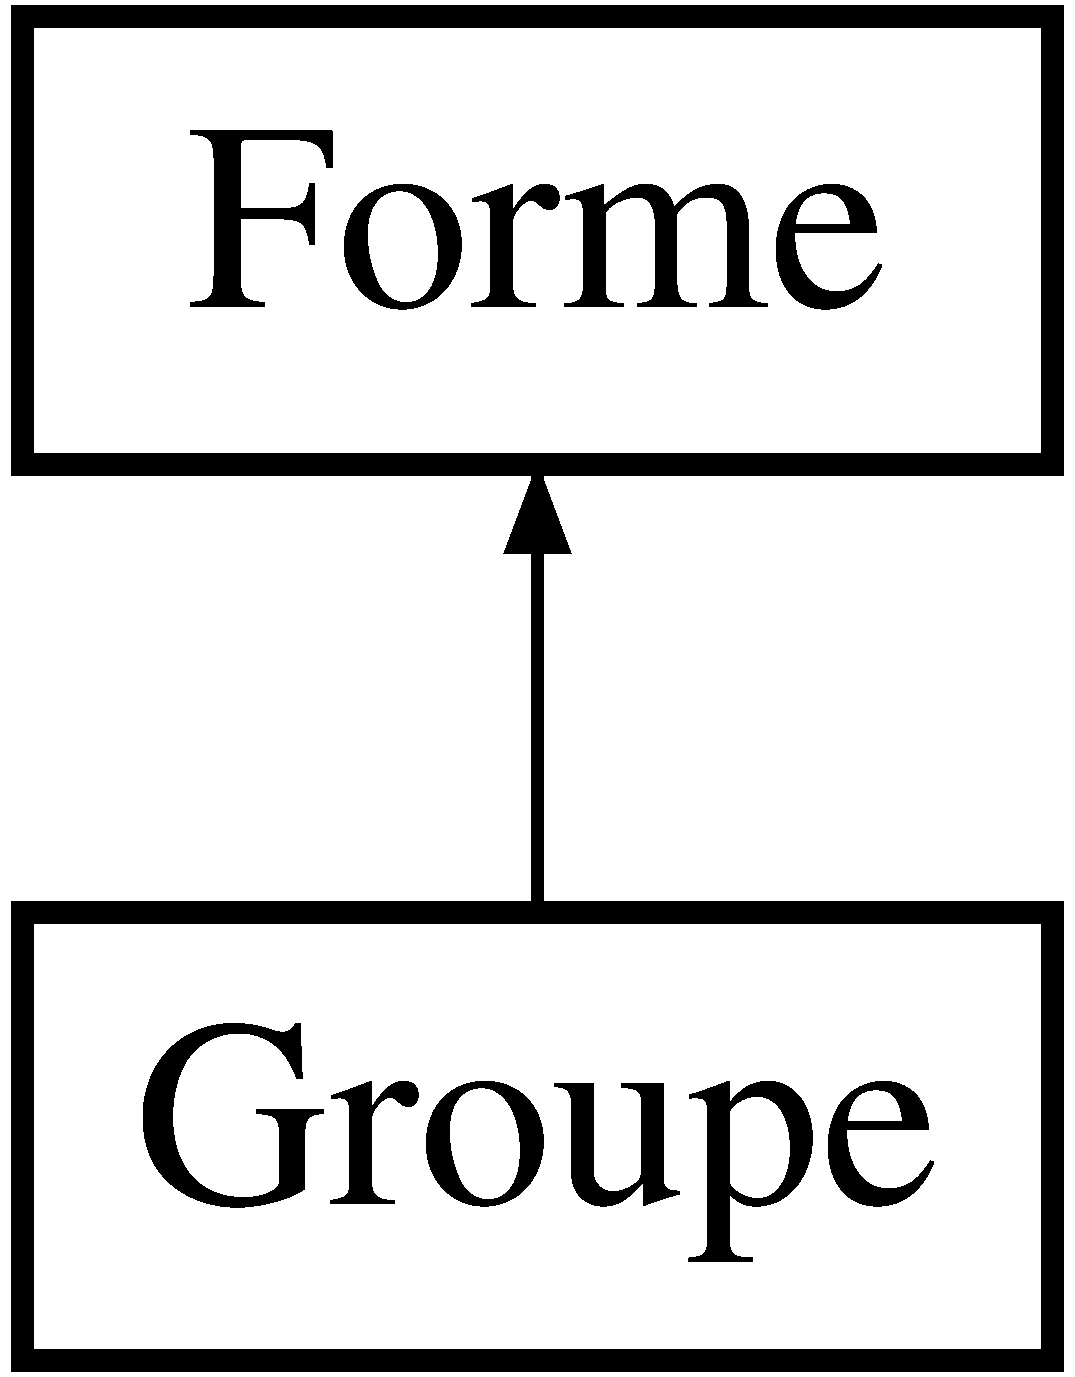
\includegraphics[height=2.000000cm]{class_groupe}
\end{center}
\end{figure}
\subsection*{Fonctions membres publiques}
\begin{DoxyCompactItemize}
\item 
\mbox{\Hypertarget{class_groupe_a413ae785f3c78828334b2f3140d2dd7a}\label{class_groupe_a413ae785f3c78828334b2f3140d2dd7a}} 
\mbox{\hyperlink{class_groupe_a413ae785f3c78828334b2f3140d2dd7a}{Groupe}} ()
\begin{DoxyCompactList}\small\item\em Constructeur par d�faut d\textquotesingle{}un groupe (vide) \end{DoxyCompactList}\item 
\mbox{\hyperlink{class_groupe_a361071a134b5d41f53421caa164724a3}{Groupe}} (const \mbox{\hyperlink{class_couleur}{Couleur}} \&coul=\mbox{\hyperlink{class_couleur}{Couleur}}())
\begin{DoxyCompactList}\small\item\em Constructeur � partir d\textquotesingle{}une couleur. \end{DoxyCompactList}\item 
\mbox{\hyperlink{class_groupe_aa2c33e88775d2459177563ad58ba4051}{Groupe}} (const \mbox{\hyperlink{class_groupe}{Groupe}} \&groupe)
\begin{DoxyCompactList}\small\item\em Constructeur dpar recopie d\textquotesingle{}un groupe. \end{DoxyCompactList}\item 
\mbox{\Hypertarget{class_groupe_a99dd414922635dcc0585aabb2a330f63}\label{class_groupe_a99dd414922635dcc0585aabb2a330f63}} 
\mbox{\hyperlink{class_groupe_a99dd414922635dcc0585aabb2a330f63}{$\sim$\+Groupe}} ()
\begin{DoxyCompactList}\small\item\em Destructeur. \end{DoxyCompactList}\item 
int \mbox{\hyperlink{class_groupe_a6835b9bfe9469390e552159538d3fa52}{get\+Nb\+Formes}} () const
\begin{DoxyCompactList}\small\item\em Getter pour r�cup�rer le nombre de formes du groupe. \end{DoxyCompactList}\item 
void \mbox{\hyperlink{class_groupe_a1ebda378e625ff7b1813fd77646b0ce8}{set\+Couleur}} (const string \&couleur)
\begin{DoxyCompactList}\small\item\em Setter pour modifier la couleur du groupe. \end{DoxyCompactList}\item 
\mbox{\Hypertarget{class_groupe_ab8bcab328da985da9907cffe76ca71d0}\label{class_groupe_ab8bcab328da985da9907cffe76ca71d0}} 
\mbox{\hyperlink{class_groupe_ab8bcab328da985da9907cffe76ca71d0}{operator string}} () const
\begin{DoxyCompactList}\small\item\em Surcharge de string pour convertir un groupe en chaine de caract�res. \end{DoxyCompactList}\item 
bool \mbox{\hyperlink{class_groupe_ab311c302878cedec3e7a2ad8705c284b}{operator==}} (const \mbox{\hyperlink{class_groupe}{Groupe}} \&obj) const
\begin{DoxyCompactList}\small\item\em Surcharge de l\textquotesingle{}op�rateur == qui teste si deux groupes sont identiques. \end{DoxyCompactList}\item 
bool \mbox{\hyperlink{class_groupe_a3671363cd8b077db5c5b2b11ea33aa4b}{operator !=}} (const \mbox{\hyperlink{class_groupe}{Groupe}} \&obj) const
\begin{DoxyCompactList}\small\item\em Surcharge de l\textquotesingle{}op�rateur !=, qui utilise ==. \end{DoxyCompactList}\item 
const \mbox{\hyperlink{class_groupe}{Groupe}} \& \mbox{\hyperlink{class_groupe_a1df9cdb57f46c67a1d20d381560201b9}{operator=}} (const \mbox{\hyperlink{class_groupe}{Groupe}} \&obj)
\begin{DoxyCompactList}\small\item\em Surcharge de l\textquotesingle{}op�rateur =, pour affecter les valeurs d\textquotesingle{}un groupe � un autre. \end{DoxyCompactList}\item 
\mbox{\hyperlink{class_forme}{Forme}} $\ast$ \mbox{\hyperlink{class_groupe_ae3a6d434a84236dfe7beaae761639350}{operator\mbox{[}$\,$\mbox{]}}} (const int indice) const
\begin{DoxyCompactList}\small\item\em Surcharge de l\textquotesingle{}op�rateur \mbox{[}\mbox{]} qui permet d\textquotesingle{}acc�der � une forme d\textquotesingle{}un groupe. \end{DoxyCompactList}\item 
\mbox{\hyperlink{class_groupe}{Groupe}} \mbox{\hyperlink{class_groupe_ad93cc28cc567226932c47bd057ead0ec}{operator+}} (\mbox{\hyperlink{class_forme}{Forme}} $\ast$f) const
\begin{DoxyCompactList}\small\item\em Surcharge de l\textquotesingle{}op�rateur + pour ajouter une forme dans un groupe. \end{DoxyCompactList}\item 
void \mbox{\hyperlink{class_groupe_adae75a5ab245624b941e5d95b0e43b60}{supprimer}} (const int indice)
\begin{DoxyCompactList}\small\item\em Supprime une forme du groupe. \end{DoxyCompactList}\item 
const double \mbox{\hyperlink{class_groupe_afc0056987479b35eedafa6cc5b758288}{get\+Aire}} () const
\begin{DoxyCompactList}\small\item\em R�cup�re l\textquotesingle{}aire totale de toutes les formes du groupe. \end{DoxyCompactList}\item 
\mbox{\hyperlink{class_forme}{Forme}} $\ast$ \mbox{\hyperlink{class_groupe_a614513db9e80b6e6c0811da16d89bb19}{clone}} () const
\begin{DoxyCompactList}\small\item\em Clone un groupe. \end{DoxyCompactList}\item 
void \mbox{\hyperlink{class_groupe_a597ef92844df8aeb27f0a47a9b3f9209}{homothetie}} (const \mbox{\hyperlink{class_vecteur2_d}{Vecteur2D}} \&vect\+Homotethie, double k)
\begin{DoxyCompactList}\small\item\em Effectue une homoth�tie directement sur le groupe. \end{DoxyCompactList}\item 
void \mbox{\hyperlink{class_groupe_a0cbd34b8d5f3d29cae4acbebd07e5af2}{translation}} (const \mbox{\hyperlink{class_vecteur2_d}{Vecteur2D}} \&vect\+Translation)
\begin{DoxyCompactList}\small\item\em Effectue une translation directement sur le groupe. \end{DoxyCompactList}\item 
void \mbox{\hyperlink{class_groupe_a4bdf9f82744057cff6706a2889c2ec68}{rotation}} (const \mbox{\hyperlink{class_vecteur2_d}{Vecteur2D}} \&vect\+Centre, double angle)
\begin{DoxyCompactList}\small\item\em Effectue une rotation directement sur le groupe. \end{DoxyCompactList}\item 
ostream \& \mbox{\hyperlink{class_groupe_a83b86a306fae5bd4dfb4461d44b5e343}{print}} (ostream \&flux) const
\begin{DoxyCompactList}\small\item\em Affiche les valeurs d\textquotesingle{}un groupe. \end{DoxyCompactList}\item 
void \mbox{\hyperlink{class_groupe_a69ab923874f5eb9ff4e0dc8dd4d359e5}{accepte\+Sauvegarder}} (const \mbox{\hyperlink{class_visiteur_sauv_t_x_t}{Visiteur\+Sauv\+T\+XT}} $\ast$v) const
\begin{DoxyCompactList}\small\item\em Appelle la m�thode visite du visiteur de sauvegarde correpondant au groupe. \end{DoxyCompactList}\item 
void \mbox{\hyperlink{class_groupe_ae62001512056945a4233c168977e9a1c}{dessiner}} (const \mbox{\hyperlink{class_visiteur_dessin}{Visiteur\+Dessin}} $\ast$v) const
\begin{DoxyCompactList}\small\item\em Appelle la m�thode visite du visiteur de dessins correpondant au groupe. \end{DoxyCompactList}\end{DoxyCompactItemize}


\subsection{Documentation des constructeurs et destructeur}
\mbox{\Hypertarget{class_groupe_a361071a134b5d41f53421caa164724a3}\label{class_groupe_a361071a134b5d41f53421caa164724a3}} 
\index{Groupe@{Groupe}!Groupe@{Groupe}}
\index{Groupe@{Groupe}!Groupe@{Groupe}}
\subsubsection{\texorpdfstring{Groupe()}{Groupe()}\hspace{0.1cm}{\footnotesize\ttfamily [1/2]}}
{\footnotesize\ttfamily Groupe\+::\+Groupe (\begin{DoxyParamCaption}\item[{const \mbox{\hyperlink{class_couleur}{Couleur}} \&}]{coul = {\ttfamily \mbox{\hyperlink{class_couleur}{Couleur}}()} }\end{DoxyParamCaption})}



Constructeur � partir d\textquotesingle{}une couleur. 


\begin{DoxyParams}{Paramètres}
{\em coul} & \mbox{\hyperlink{class_couleur}{Couleur}} \\
\hline
\end{DoxyParams}
\mbox{\Hypertarget{class_groupe_aa2c33e88775d2459177563ad58ba4051}\label{class_groupe_aa2c33e88775d2459177563ad58ba4051}} 
\index{Groupe@{Groupe}!Groupe@{Groupe}}
\index{Groupe@{Groupe}!Groupe@{Groupe}}
\subsubsection{\texorpdfstring{Groupe()}{Groupe()}\hspace{0.1cm}{\footnotesize\ttfamily [2/2]}}
{\footnotesize\ttfamily Groupe\+::\+Groupe (\begin{DoxyParamCaption}\item[{const \mbox{\hyperlink{class_groupe}{Groupe}} \&}]{groupe }\end{DoxyParamCaption})}



Constructeur dpar recopie d\textquotesingle{}un groupe. 


\begin{DoxyParams}{Paramètres}
{\em groupe} & \mbox{\hyperlink{class_groupe}{Groupe}} � recopier \\
\hline
\end{DoxyParams}


\subsection{Documentation des fonctions membres}
\mbox{\Hypertarget{class_groupe_a69ab923874f5eb9ff4e0dc8dd4d359e5}\label{class_groupe_a69ab923874f5eb9ff4e0dc8dd4d359e5}} 
\index{Groupe@{Groupe}!accepteSauvegarder@{accepteSauvegarder}}
\index{accepteSauvegarder@{accepteSauvegarder}!Groupe@{Groupe}}
\subsubsection{\texorpdfstring{accepteSauvegarder()}{accepteSauvegarder()}}
{\footnotesize\ttfamily void Groupe\+::accepte\+Sauvegarder (\begin{DoxyParamCaption}\item[{const \mbox{\hyperlink{class_visiteur_sauv_t_x_t}{Visiteur\+Sauv\+T\+XT}} $\ast$}]{v }\end{DoxyParamCaption}) const\hspace{0.3cm}{\ttfamily [virtual]}}



Appelle la m�thode visite du visiteur de sauvegarde correpondant au groupe. 


\begin{DoxyParams}{Paramètres}
{\em v} & Pointeur sur le visiteur de sauvegarde \\
\hline
\end{DoxyParams}


Implémente \mbox{\hyperlink{class_forme_a7be10bca98001dc368adc3a3e93d0f48}{Forme}}.

\mbox{\Hypertarget{class_groupe_a614513db9e80b6e6c0811da16d89bb19}\label{class_groupe_a614513db9e80b6e6c0811da16d89bb19}} 
\index{Groupe@{Groupe}!clone@{clone}}
\index{clone@{clone}!Groupe@{Groupe}}
\subsubsection{\texorpdfstring{clone()}{clone()}}
{\footnotesize\ttfamily \mbox{\hyperlink{class_forme}{Forme}} $\ast$ Groupe\+::clone (\begin{DoxyParamCaption}{ }\end{DoxyParamCaption}) const\hspace{0.3cm}{\ttfamily [virtual]}}



Clone un groupe. 

\begin{DoxyReturn}{Renvoie}
Forme$\ast$ Pointeur sur le groupe clon� 
\end{DoxyReturn}


Implémente \mbox{\hyperlink{class_forme_a226750dc3f772514fe58e1dc16f3d0d5}{Forme}}.

\mbox{\Hypertarget{class_groupe_ae62001512056945a4233c168977e9a1c}\label{class_groupe_ae62001512056945a4233c168977e9a1c}} 
\index{Groupe@{Groupe}!dessiner@{dessiner}}
\index{dessiner@{dessiner}!Groupe@{Groupe}}
\subsubsection{\texorpdfstring{dessiner()}{dessiner()}}
{\footnotesize\ttfamily void Groupe\+::dessiner (\begin{DoxyParamCaption}\item[{const \mbox{\hyperlink{class_visiteur_dessin}{Visiteur\+Dessin}} $\ast$}]{v }\end{DoxyParamCaption}) const\hspace{0.3cm}{\ttfamily [virtual]}}



Appelle la m�thode visite du visiteur de dessins correpondant au groupe. 


\begin{DoxyParams}{Paramètres}
{\em v} & Pointeur sur le visiteur de dessin \\
\hline
\end{DoxyParams}


Implémente \mbox{\hyperlink{class_forme_a8cd4879a6a5751cbf6d3bbbfbec41566}{Forme}}.

\mbox{\Hypertarget{class_groupe_afc0056987479b35eedafa6cc5b758288}\label{class_groupe_afc0056987479b35eedafa6cc5b758288}} 
\index{Groupe@{Groupe}!getAire@{getAire}}
\index{getAire@{getAire}!Groupe@{Groupe}}
\subsubsection{\texorpdfstring{getAire()}{getAire()}}
{\footnotesize\ttfamily const double Groupe\+::get\+Aire (\begin{DoxyParamCaption}{ }\end{DoxyParamCaption}) const\hspace{0.3cm}{\ttfamily [virtual]}}



R�cup�re l\textquotesingle{}aire totale de toutes les formes du groupe. 

\begin{DoxyReturn}{Renvoie}
R�el Somme de l\textquotesingle{}aire de toutes les formes du groupe 
\end{DoxyReturn}


Implémente \mbox{\hyperlink{class_forme_adf4346150d8f734d7a48f7661e30cab4}{Forme}}.

\mbox{\Hypertarget{class_groupe_a6835b9bfe9469390e552159538d3fa52}\label{class_groupe_a6835b9bfe9469390e552159538d3fa52}} 
\index{Groupe@{Groupe}!getNbFormes@{getNbFormes}}
\index{getNbFormes@{getNbFormes}!Groupe@{Groupe}}
\subsubsection{\texorpdfstring{getNbFormes()}{getNbFormes()}}
{\footnotesize\ttfamily int Groupe\+::get\+Nb\+Formes (\begin{DoxyParamCaption}{ }\end{DoxyParamCaption}) const}



Getter pour r�cup�rer le nombre de formes du groupe. 

\begin{DoxyReturn}{Renvoie}
int Nombre de formes du groupe 
\end{DoxyReturn}
\mbox{\Hypertarget{class_groupe_a597ef92844df8aeb27f0a47a9b3f9209}\label{class_groupe_a597ef92844df8aeb27f0a47a9b3f9209}} 
\index{Groupe@{Groupe}!homothetie@{homothetie}}
\index{homothetie@{homothetie}!Groupe@{Groupe}}
\subsubsection{\texorpdfstring{homothetie()}{homothetie()}}
{\footnotesize\ttfamily void Groupe\+::homothetie (\begin{DoxyParamCaption}\item[{const \mbox{\hyperlink{class_vecteur2_d}{Vecteur2D}} \&}]{vect\+Homotethie,  }\item[{double}]{k }\end{DoxyParamCaption})\hspace{0.3cm}{\ttfamily [virtual]}}



Effectue une homoth�tie directement sur le groupe. 


\begin{DoxyParams}{Paramètres}
{\em vect\+Homothetie} & \mbox{\hyperlink{class_vecteur2_d}{Vecteur2D}} \\
\hline
{\em k} & R�el \\
\hline
\end{DoxyParams}


Implémente \mbox{\hyperlink{class_forme_aeaae98ea3de8523de9ba9093e19779d8}{Forme}}.

\mbox{\Hypertarget{class_groupe_a3671363cd8b077db5c5b2b11ea33aa4b}\label{class_groupe_a3671363cd8b077db5c5b2b11ea33aa4b}} 
\index{Groupe@{Groupe}!operator "!=@{operator "!=}}
\index{operator "!=@{operator "!=}!Groupe@{Groupe}}
\subsubsection{\texorpdfstring{operator "!=()}{operator !=()}}
{\footnotesize\ttfamily bool Groupe\+::operator != (\begin{DoxyParamCaption}\item[{const \mbox{\hyperlink{class_groupe}{Groupe}} \&}]{obj }\end{DoxyParamCaption}) const}



Surcharge de l\textquotesingle{}op�rateur !=, qui utilise ==. 


\begin{DoxyParams}{Paramètres}
{\em obj} & \mbox{\hyperlink{class_groupe}{Groupe}} � comparer \\
\hline
\end{DoxyParams}
\begin{DoxyReturn}{Renvoie}
bool Bool�en vrai si les deux groupes sont diff�rents, faux sinon 
\end{DoxyReturn}
\mbox{\Hypertarget{class_groupe_ad93cc28cc567226932c47bd057ead0ec}\label{class_groupe_ad93cc28cc567226932c47bd057ead0ec}} 
\index{Groupe@{Groupe}!operator+@{operator+}}
\index{operator+@{operator+}!Groupe@{Groupe}}
\subsubsection{\texorpdfstring{operator+()}{operator+()}}
{\footnotesize\ttfamily \mbox{\hyperlink{class_groupe}{Groupe}} Groupe\+::operator+ (\begin{DoxyParamCaption}\item[{\mbox{\hyperlink{class_forme}{Forme}} $\ast$}]{f }\end{DoxyParamCaption}) const}



Surcharge de l\textquotesingle{}op�rateur + pour ajouter une forme dans un groupe. 


\begin{DoxyParams}{Paramètres}
{\em f} & Pointeur sur la forme � ajouter au groupe \\
\hline
\end{DoxyParams}
\begin{DoxyReturn}{Renvoie}
\mbox{\hyperlink{class_groupe}{Groupe}} Copie du nouveau groupe avec la nouvelle forme ajout�e 
\end{DoxyReturn}
\mbox{\Hypertarget{class_groupe_a1df9cdb57f46c67a1d20d381560201b9}\label{class_groupe_a1df9cdb57f46c67a1d20d381560201b9}} 
\index{Groupe@{Groupe}!operator=@{operator=}}
\index{operator=@{operator=}!Groupe@{Groupe}}
\subsubsection{\texorpdfstring{operator=()}{operator=()}}
{\footnotesize\ttfamily const \mbox{\hyperlink{class_groupe}{Groupe}} \& Groupe\+::operator= (\begin{DoxyParamCaption}\item[{const \mbox{\hyperlink{class_groupe}{Groupe}} \&}]{obj }\end{DoxyParamCaption})}



Surcharge de l\textquotesingle{}op�rateur =, pour affecter les valeurs d\textquotesingle{}un groupe � un autre. 


\begin{DoxyParams}{Paramètres}
{\em obj} & Objet � copier \\
\hline
\end{DoxyParams}
\begin{DoxyReturn}{Renvoie}
obj La resultante de l\textquotesingle{}affectation du groupe 
\end{DoxyReturn}
\mbox{\Hypertarget{class_groupe_ab311c302878cedec3e7a2ad8705c284b}\label{class_groupe_ab311c302878cedec3e7a2ad8705c284b}} 
\index{Groupe@{Groupe}!operator==@{operator==}}
\index{operator==@{operator==}!Groupe@{Groupe}}
\subsubsection{\texorpdfstring{operator==()}{operator==()}}
{\footnotesize\ttfamily bool Groupe\+::operator== (\begin{DoxyParamCaption}\item[{const \mbox{\hyperlink{class_groupe}{Groupe}} \&}]{obj }\end{DoxyParamCaption}) const}



Surcharge de l\textquotesingle{}op�rateur == qui teste si deux groupes sont identiques. 


\begin{DoxyParams}{Paramètres}
{\em obj} & \mbox{\hyperlink{class_groupe}{Groupe}} � comparer \\
\hline
\end{DoxyParams}
\begin{DoxyReturn}{Renvoie}
bool Bool�en vrai si les deux groupes sont identiques, faux sinon 
\end{DoxyReturn}
\mbox{\Hypertarget{class_groupe_ae3a6d434a84236dfe7beaae761639350}\label{class_groupe_ae3a6d434a84236dfe7beaae761639350}} 
\index{Groupe@{Groupe}!operator\mbox{[}\mbox{]}@{operator[]}}
\index{operator\mbox{[}\mbox{]}@{operator[]}!Groupe@{Groupe}}
\subsubsection{\texorpdfstring{operator[]()}{operator[]()}}
{\footnotesize\ttfamily \mbox{\hyperlink{class_forme}{Forme}} $\ast$ Groupe\+::operator\mbox{[}$\,$\mbox{]} (\begin{DoxyParamCaption}\item[{const int}]{indice }\end{DoxyParamCaption}) const}



Surcharge de l\textquotesingle{}op�rateur \mbox{[}\mbox{]} qui permet d\textquotesingle{}acc�der � une forme d\textquotesingle{}un groupe. 


\begin{DoxyParams}{Paramètres}
{\em indice} & Indice de la forme � r�cup�rer \textbackslash{}return\+Forme$\ast$ Un pointeur sur la forme se trouvant � l\textquotesingle{}indice donn� en param�tre \\
\hline
\end{DoxyParams}
\mbox{\Hypertarget{class_groupe_a83b86a306fae5bd4dfb4461d44b5e343}\label{class_groupe_a83b86a306fae5bd4dfb4461d44b5e343}} 
\index{Groupe@{Groupe}!print@{print}}
\index{print@{print}!Groupe@{Groupe}}
\subsubsection{\texorpdfstring{print()}{print()}}
{\footnotesize\ttfamily ostream \& Groupe\+::print (\begin{DoxyParamCaption}\item[{ostream \&}]{flux }\end{DoxyParamCaption}) const\hspace{0.3cm}{\ttfamily [virtual]}}



Affiche les valeurs d\textquotesingle{}un groupe. 


\begin{DoxyParams}{Paramètres}
{\em flux} & Flux de sortie \\
\hline
\end{DoxyParams}
\begin{DoxyReturn}{Renvoie}
ostream F\+Lux de sortie 
\end{DoxyReturn}


Réimplémentée à partir de \mbox{\hyperlink{class_forme_a348a12ae03fe2167ffd586f4deae6c76}{Forme}}.

\mbox{\Hypertarget{class_groupe_a4bdf9f82744057cff6706a2889c2ec68}\label{class_groupe_a4bdf9f82744057cff6706a2889c2ec68}} 
\index{Groupe@{Groupe}!rotation@{rotation}}
\index{rotation@{rotation}!Groupe@{Groupe}}
\subsubsection{\texorpdfstring{rotation()}{rotation()}}
{\footnotesize\ttfamily void Groupe\+::rotation (\begin{DoxyParamCaption}\item[{const \mbox{\hyperlink{class_vecteur2_d}{Vecteur2D}} \&}]{vect\+Centre,  }\item[{double}]{angle }\end{DoxyParamCaption})\hspace{0.3cm}{\ttfamily [virtual]}}



Effectue une rotation directement sur le groupe. 


\begin{DoxyParams}{Paramètres}
{\em vect\+Centre} & \mbox{\hyperlink{class_vecteur2_d}{Vecteur2D}} \\
\hline
{\em angle} & R�el \\
\hline
\end{DoxyParams}


Implémente \mbox{\hyperlink{class_forme_af17c4156d00281b4b62d8c27dcb75569}{Forme}}.

\mbox{\Hypertarget{class_groupe_a1ebda378e625ff7b1813fd77646b0ce8}\label{class_groupe_a1ebda378e625ff7b1813fd77646b0ce8}} 
\index{Groupe@{Groupe}!setCouleur@{setCouleur}}
\index{setCouleur@{setCouleur}!Groupe@{Groupe}}
\subsubsection{\texorpdfstring{setCouleur()}{setCouleur()}}
{\footnotesize\ttfamily void Groupe\+::set\+Couleur (\begin{DoxyParamCaption}\item[{const string \&}]{couleur }\end{DoxyParamCaption})}



Setter pour modifier la couleur du groupe. 


\begin{DoxyParams}{Paramètres}
{\em couleur} & Chaine de caract�res correspondant � la couleur \\
\hline
\end{DoxyParams}
\mbox{\Hypertarget{class_groupe_adae75a5ab245624b941e5d95b0e43b60}\label{class_groupe_adae75a5ab245624b941e5d95b0e43b60}} 
\index{Groupe@{Groupe}!supprimer@{supprimer}}
\index{supprimer@{supprimer}!Groupe@{Groupe}}
\subsubsection{\texorpdfstring{supprimer()}{supprimer()}}
{\footnotesize\ttfamily void Groupe\+::supprimer (\begin{DoxyParamCaption}\item[{const int}]{indice }\end{DoxyParamCaption})}



Supprime une forme du groupe. 


\begin{DoxyParams}{Paramètres}
{\em indice} & Indice de la forme � supprimer \\
\hline
\end{DoxyParams}
\mbox{\Hypertarget{class_groupe_a0cbd34b8d5f3d29cae4acbebd07e5af2}\label{class_groupe_a0cbd34b8d5f3d29cae4acbebd07e5af2}} 
\index{Groupe@{Groupe}!translation@{translation}}
\index{translation@{translation}!Groupe@{Groupe}}
\subsubsection{\texorpdfstring{translation()}{translation()}}
{\footnotesize\ttfamily void Groupe\+::translation (\begin{DoxyParamCaption}\item[{const \mbox{\hyperlink{class_vecteur2_d}{Vecteur2D}} \&}]{vect\+Translation }\end{DoxyParamCaption})\hspace{0.3cm}{\ttfamily [virtual]}}



Effectue une translation directement sur le groupe. 


\begin{DoxyParams}{Paramètres}
{\em vect\+Translation} & \mbox{\hyperlink{class_vecteur2_d}{Vecteur2D}} \\
\hline
\end{DoxyParams}


Implémente \mbox{\hyperlink{class_forme_ad156a02098ef453b09919b2a3156f607}{Forme}}.



La documentation de cette classe a été générée à partir des fichiers suivants \+:\begin{DoxyCompactItemize}
\item 
\mbox{\hyperlink{_groupe_8h}{Groupe.\+h}}\item 
Groupe.\+cpp\end{DoxyCompactItemize}

\hypertarget{class_polygone}{}\section{Polygone Class Reference}
\label{class_polygone}\index{Polygone@{Polygone}}


{\ttfamily \#include $<$Polygone.\+h$>$}

Inheritance diagram for Polygone\+:\begin{figure}[H]
\begin{center}
\leavevmode
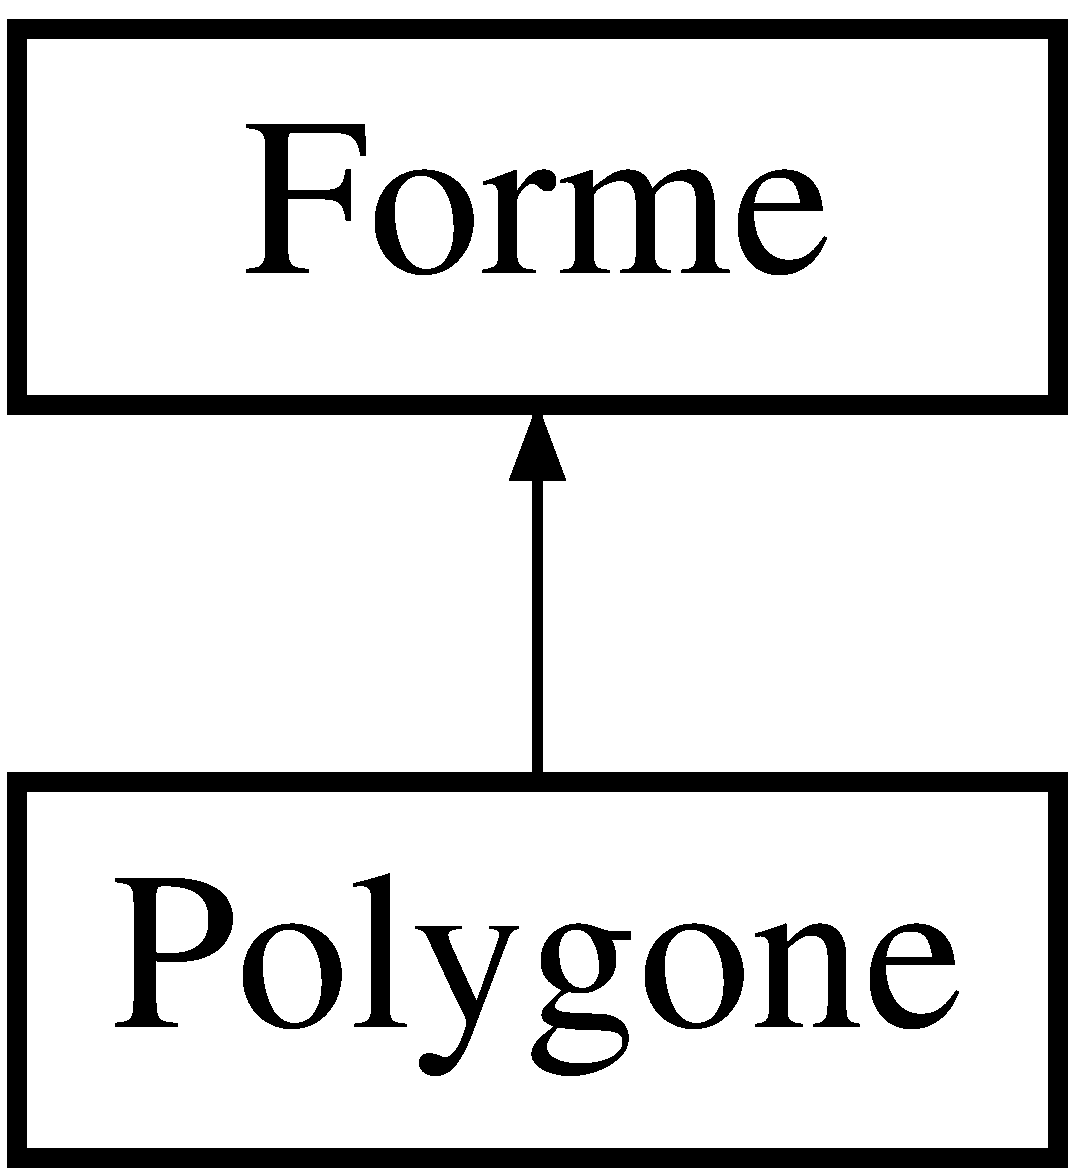
\includegraphics[height=2.000000cm]{class_polygone}
\end{center}
\end{figure}
\subsection*{Public Member Functions}
\begin{DoxyCompactItemize}
\item 
\hyperlink{class_polygone_ac1b10c1081562f05186668b324d25162}{Polygone} (const \hyperlink{class_vecteur2_d}{Vecteur2D} \&P1, const \hyperlink{class_vecteur2_d}{Vecteur2D} \&P2, const \hyperlink{class_vecteur2_d}{Vecteur2D} \&P3, const \hyperlink{class_couleur}{Couleur} \&coul=\hyperlink{class_couleur}{Couleur}())
\begin{DoxyCompactList}\small\item\em Constructeur � partir de 3 points et d\textquotesingle{}une couleur par d�faut. \end{DoxyCompactList}\item 
\hyperlink{class_polygone_a7acb9caaba3f6ff57ff7279a8ead1bfe}{Polygone} (const \hyperlink{class_polygone}{Polygone} \&\hyperlink{class_polygone}{Polygone})
\begin{DoxyCompactList}\small\item\em Constructeur par recopie d\textquotesingle{}un polygone. \end{DoxyCompactList}\item 
\hyperlink{class_polygone_ae293043ea9d180259771515a6496cd8c}{$\sim$\+Polygone} ()
\begin{DoxyCompactList}\small\item\em Destructeur. \end{DoxyCompactList}\item 
int \hyperlink{class_polygone_a1487d8c92753d1a596583d130b12993e}{get\+Nb\+Points} () const
\begin{DoxyCompactList}\small\item\em Getter pour savoir le nombre de points dans le polygone. \end{DoxyCompactList}\item 
bool \hyperlink{class_polygone_ae33d91c0571f9ecf3178ce02fa35cb3a}{verif\+Points} (vector$<$ \hyperlink{class_vecteur2_d}{Vecteur2D} $>$ \&tab\+Points)
\begin{DoxyCompactList}\small\item\em V�rifie si tous les points sont correctement plac�s \end{DoxyCompactList}\item 
\hyperlink{class_polygone_abd801a84b5306df8021f1571d82deafd}{operator string} () const
\begin{DoxyCompactList}\small\item\em Surcharge de l\textquotesingle{}op�rateur string pour convertir un polygone en string. \end{DoxyCompactList}\item 
bool \hyperlink{class_polygone_aa9ea8cf2208263f4a22f1a1ebae5816b}{operator==} (const \hyperlink{class_polygone}{Polygone} \&objet) const
\begin{DoxyCompactList}\small\item\em Surcharge de l\textquotesingle{}op�rateur == qui teste si deux polygones sont identiques. \end{DoxyCompactList}\item 
bool \hyperlink{class_polygone_a97a853574dd818c0c49812e31d047b06}{operator!=} (const \hyperlink{class_polygone}{Polygone} \&objet) const
\begin{DoxyCompactList}\small\item\em Surcharge de l\textquotesingle{}op�rateur !=, qui utilise ==. \end{DoxyCompactList}\item 
const \hyperlink{class_polygone}{Polygone} \& \hyperlink{class_polygone_a85a19a58dcc1110a345a0340156902fb}{operator=} (const \hyperlink{class_polygone}{Polygone} \&obj)
\begin{DoxyCompactList}\small\item\em Surcharge de l\textquotesingle{}op�rateur =, pour affecter les valeurs d\textquotesingle{}un polygone � un autre. \end{DoxyCompactList}\item 
const \hyperlink{class_vecteur2_d}{Vecteur2D} \& \hyperlink{class_polygone_a94361c66706ba1bb01b54dd563069783}{operator\mbox{[}$\,$\mbox{]}} (int indice) const
\begin{DoxyCompactList}\small\item\em Surcharge de l\textquotesingle{}op�rateur \mbox{[}\mbox{]} pour acc�der � un point du polygone par son indice. \end{DoxyCompactList}\item 
\hyperlink{class_polygone}{Polygone} \hyperlink{class_polygone_aba485c4d7cfffd70b3ce7bf53a4fdb93}{operator+} (const \hyperlink{class_vecteur2_d}{Vecteur2D} \&v) const
\begin{DoxyCompactList}\small\item\em Surcharge de l\textquotesingle{}op�rateur + pour ajouter un point au polygone. \end{DoxyCompactList}\item 
void \hyperlink{class_polygone_a88cdddc933f9bea8583c668a5935cca0}{supprimer} (int indice)
\begin{DoxyCompactList}\small\item\em Supprime un pointdu polygone. \end{DoxyCompactList}\item 
const double \hyperlink{class_polygone_a07880a169f0241140d15cdbca13a3622}{get\+Aire} () const
\begin{DoxyCompactList}\small\item\em Getter pour r�cup�rer l\textquotesingle{}aire du polygone. \end{DoxyCompactList}\item 
\hyperlink{class_forme}{Forme} $\ast$ \hyperlink{class_polygone_a3efc2ac3ad92c3609f6d5f8fe9039871}{clone} () const
\begin{DoxyCompactList}\small\item\em Clone un polygone. \end{DoxyCompactList}\item 
void \hyperlink{class_polygone_a211ccacc83e547e0b7cd129e23e8cf1d}{homothetie} (const \hyperlink{class_vecteur2_d}{Vecteur2D} \&vect\+Homotethie, double k)
\begin{DoxyCompactList}\small\item\em Effectue une homoth�tie directement sur le polygone. \end{DoxyCompactList}\item 
void \hyperlink{class_polygone_a4c4e05250d5ebebbb3d544011be0dbd7}{translation} (const \hyperlink{class_vecteur2_d}{Vecteur2D} \&vect\+Translation)
\begin{DoxyCompactList}\small\item\em Effectue une translation directement sur le polygone. \end{DoxyCompactList}\item 
void \hyperlink{class_polygone_a5f30d9d61cfc6c3f2cafd345f8fc8824}{rotation} (const \hyperlink{class_vecteur2_d}{Vecteur2D} \&vect\+Centre, double angle)
\begin{DoxyCompactList}\small\item\em Effectue une rotation directement sur le polygone. \end{DoxyCompactList}\item 
ostream \& \hyperlink{class_polygone_a3c8534deace725beaaaa0657ad720822}{print} (ostream \&flux) const
\begin{DoxyCompactList}\small\item\em Affiche les valeurs d\textquotesingle{}un polygone. \end{DoxyCompactList}\item 
void \hyperlink{class_polygone_af97fb141e2b4b0042c8f0998b0499af3}{accepte\+Sauvegarder} (const \hyperlink{class_visiteur_sauv_t_x_t}{Visiteur\+Sauv\+T\+XT} $\ast$v) const
\begin{DoxyCompactList}\small\item\em Appelle la m�thode visite du visiteur de sauvegarde correpondant au polygone. \end{DoxyCompactList}\item 
void \hyperlink{class_polygone_a2e71a18fa658499da019558913e7ccbb}{dessiner} (const \hyperlink{class_visiteur_dessin}{Visiteur\+Dessin} $\ast$v) const
\begin{DoxyCompactList}\small\item\em Appelle la m�thode visite du visiteur de dessin correpondant au polygone. \end{DoxyCompactList}\end{DoxyCompactItemize}


\subsection{Constructor \& Destructor Documentation}
\mbox{\Hypertarget{class_polygone_ac1b10c1081562f05186668b324d25162}\label{class_polygone_ac1b10c1081562f05186668b324d25162}} 
\index{Polygone@{Polygone}!Polygone@{Polygone}}
\index{Polygone@{Polygone}!Polygone@{Polygone}}
\subsubsection{\texorpdfstring{Polygone()}{Polygone()}\hspace{0.1cm}{\footnotesize\ttfamily [1/2]}}
{\footnotesize\ttfamily Polygone\+::\+Polygone (\begin{DoxyParamCaption}\item[{const \hyperlink{class_vecteur2_d}{Vecteur2D} \&}]{P1,  }\item[{const \hyperlink{class_vecteur2_d}{Vecteur2D} \&}]{P2,  }\item[{const \hyperlink{class_vecteur2_d}{Vecteur2D} \&}]{P3,  }\item[{const \hyperlink{class_couleur}{Couleur} \&}]{coul = {\ttfamily \hyperlink{class_couleur}{Couleur}()} }\end{DoxyParamCaption})}



Constructeur � partir de 3 points et d\textquotesingle{}une couleur par d�faut. 


\begin{DoxyParams}{Parameters}
{\em P1} & \hyperlink{class_vecteur2_d}{Vecteur2D} \\
\hline
{\em P2} & vecteur2D \\
\hline
{\em P3} & \hyperlink{class_vecteur2_d}{Vecteur2D} \\
\hline
\end{DoxyParams}
\mbox{\Hypertarget{class_polygone_a7acb9caaba3f6ff57ff7279a8ead1bfe}\label{class_polygone_a7acb9caaba3f6ff57ff7279a8ead1bfe}} 
\index{Polygone@{Polygone}!Polygone@{Polygone}}
\index{Polygone@{Polygone}!Polygone@{Polygone}}
\subsubsection{\texorpdfstring{Polygone()}{Polygone()}\hspace{0.1cm}{\footnotesize\ttfamily [2/2]}}
{\footnotesize\ttfamily Polygone\+::\+Polygone (\begin{DoxyParamCaption}\item[{const \hyperlink{class_polygone}{Polygone} \&}]{Polygone }\end{DoxyParamCaption})}



Constructeur par recopie d\textquotesingle{}un polygone. 


\begin{DoxyParams}{Parameters}
{\em \hyperlink{class_polygone}{Polygone}} & Le polygone � recopier \\
\hline
\end{DoxyParams}
\mbox{\Hypertarget{class_polygone_ae293043ea9d180259771515a6496cd8c}\label{class_polygone_ae293043ea9d180259771515a6496cd8c}} 
\index{Polygone@{Polygone}!````~Polygone@{$\sim$\+Polygone}}
\index{````~Polygone@{$\sim$\+Polygone}!Polygone@{Polygone}}
\subsubsection{\texorpdfstring{$\sim$\+Polygone()}{~Polygone()}}
{\footnotesize\ttfamily Polygone\+::$\sim$\+Polygone (\begin{DoxyParamCaption}{ }\end{DoxyParamCaption})}



Destructeur. 



\subsection{Member Function Documentation}
\mbox{\Hypertarget{class_polygone_af97fb141e2b4b0042c8f0998b0499af3}\label{class_polygone_af97fb141e2b4b0042c8f0998b0499af3}} 
\index{Polygone@{Polygone}!accepte\+Sauvegarder@{accepte\+Sauvegarder}}
\index{accepte\+Sauvegarder@{accepte\+Sauvegarder}!Polygone@{Polygone}}
\subsubsection{\texorpdfstring{accepte\+Sauvegarder()}{accepteSauvegarder()}}
{\footnotesize\ttfamily void Polygone\+::accepte\+Sauvegarder (\begin{DoxyParamCaption}\item[{const \hyperlink{class_visiteur_sauv_t_x_t}{Visiteur\+Sauv\+T\+XT} $\ast$}]{v }\end{DoxyParamCaption}) const\hspace{0.3cm}{\ttfamily [virtual]}}



Appelle la m�thode visite du visiteur de sauvegarde correpondant au polygone. 


\begin{DoxyParams}{Parameters}
{\em v} & Pointeur sur le visiteur de sauvegarde \\
\hline
\end{DoxyParams}


Implements \hyperlink{class_forme_a7be10bca98001dc368adc3a3e93d0f48}{Forme}.

\mbox{\Hypertarget{class_polygone_a3efc2ac3ad92c3609f6d5f8fe9039871}\label{class_polygone_a3efc2ac3ad92c3609f6d5f8fe9039871}} 
\index{Polygone@{Polygone}!clone@{clone}}
\index{clone@{clone}!Polygone@{Polygone}}
\subsubsection{\texorpdfstring{clone()}{clone()}}
{\footnotesize\ttfamily \hyperlink{class_forme}{Forme} $\ast$ Polygone\+::clone (\begin{DoxyParamCaption}{ }\end{DoxyParamCaption}) const\hspace{0.3cm}{\ttfamily [virtual]}}



Clone un polygone. 

\begin{DoxyReturn}{Returns}
Forme$\ast$ Pointeur sur le polygone clon� 
\end{DoxyReturn}


Implements \hyperlink{class_forme_a226750dc3f772514fe58e1dc16f3d0d5}{Forme}.

\mbox{\Hypertarget{class_polygone_a2e71a18fa658499da019558913e7ccbb}\label{class_polygone_a2e71a18fa658499da019558913e7ccbb}} 
\index{Polygone@{Polygone}!dessiner@{dessiner}}
\index{dessiner@{dessiner}!Polygone@{Polygone}}
\subsubsection{\texorpdfstring{dessiner()}{dessiner()}}
{\footnotesize\ttfamily void Polygone\+::dessiner (\begin{DoxyParamCaption}\item[{const \hyperlink{class_visiteur_dessin}{Visiteur\+Dessin} $\ast$}]{v }\end{DoxyParamCaption}) const\hspace{0.3cm}{\ttfamily [virtual]}}



Appelle la m�thode visite du visiteur de dessin correpondant au polygone. 


\begin{DoxyParams}{Parameters}
{\em v} & Pointeur sur le visiteur de dessin \\
\hline
\end{DoxyParams}


Implements \hyperlink{class_forme_a8cd4879a6a5751cbf6d3bbbfbec41566}{Forme}.

\mbox{\Hypertarget{class_polygone_a07880a169f0241140d15cdbca13a3622}\label{class_polygone_a07880a169f0241140d15cdbca13a3622}} 
\index{Polygone@{Polygone}!get\+Aire@{get\+Aire}}
\index{get\+Aire@{get\+Aire}!Polygone@{Polygone}}
\subsubsection{\texorpdfstring{get\+Aire()}{getAire()}}
{\footnotesize\ttfamily const double Polygone\+::get\+Aire (\begin{DoxyParamCaption}{ }\end{DoxyParamCaption}) const\hspace{0.3cm}{\ttfamily [virtual]}}



Getter pour r�cup�rer l\textquotesingle{}aire du polygone. 

\begin{DoxyReturn}{Returns}
R�el L\textquotesingle{}aire du polygone 
\end{DoxyReturn}


Implements \hyperlink{class_forme_adf4346150d8f734d7a48f7661e30cab4}{Forme}.

\mbox{\Hypertarget{class_polygone_a1487d8c92753d1a596583d130b12993e}\label{class_polygone_a1487d8c92753d1a596583d130b12993e}} 
\index{Polygone@{Polygone}!get\+Nb\+Points@{get\+Nb\+Points}}
\index{get\+Nb\+Points@{get\+Nb\+Points}!Polygone@{Polygone}}
\subsubsection{\texorpdfstring{get\+Nb\+Points()}{getNbPoints()}}
{\footnotesize\ttfamily int Polygone\+::get\+Nb\+Points (\begin{DoxyParamCaption}{ }\end{DoxyParamCaption}) const}



Getter pour savoir le nombre de points dans le polygone. 

\begin{DoxyReturn}{Returns}
int le bombre de points 
\end{DoxyReturn}
\mbox{\Hypertarget{class_polygone_a211ccacc83e547e0b7cd129e23e8cf1d}\label{class_polygone_a211ccacc83e547e0b7cd129e23e8cf1d}} 
\index{Polygone@{Polygone}!homothetie@{homothetie}}
\index{homothetie@{homothetie}!Polygone@{Polygone}}
\subsubsection{\texorpdfstring{homothetie()}{homothetie()}}
{\footnotesize\ttfamily void Polygone\+::homothetie (\begin{DoxyParamCaption}\item[{const \hyperlink{class_vecteur2_d}{Vecteur2D} \&}]{vect\+Homotethie,  }\item[{double}]{k }\end{DoxyParamCaption})\hspace{0.3cm}{\ttfamily [virtual]}}



Effectue une homoth�tie directement sur le polygone. 


\begin{DoxyParams}{Parameters}
{\em vect\+Homothetie} & \hyperlink{class_vecteur2_d}{Vecteur2D} \\
\hline
{\em k} & R�el \\
\hline
\end{DoxyParams}


Implements \hyperlink{class_forme_aeaae98ea3de8523de9ba9093e19779d8}{Forme}.

\mbox{\Hypertarget{class_polygone_abd801a84b5306df8021f1571d82deafd}\label{class_polygone_abd801a84b5306df8021f1571d82deafd}} 
\index{Polygone@{Polygone}!operator string@{operator string}}
\index{operator string@{operator string}!Polygone@{Polygone}}
\subsubsection{\texorpdfstring{operator string()}{operator string()}}
{\footnotesize\ttfamily Polygone\+::operator string (\begin{DoxyParamCaption}{ }\end{DoxyParamCaption}) const\hspace{0.3cm}{\ttfamily [virtual]}}



Surcharge de l\textquotesingle{}op�rateur string pour convertir un polygone en string. 



Reimplemented from \hyperlink{class_forme_a809375f023f0f19227f3e3821ee56731}{Forme}.

\mbox{\Hypertarget{class_polygone_a97a853574dd818c0c49812e31d047b06}\label{class_polygone_a97a853574dd818c0c49812e31d047b06}} 
\index{Polygone@{Polygone}!operator"!=@{operator"!=}}
\index{operator"!=@{operator"!=}!Polygone@{Polygone}}
\subsubsection{\texorpdfstring{operator"!=()}{operator!=()}}
{\footnotesize\ttfamily bool Polygone\+::operator!= (\begin{DoxyParamCaption}\item[{const \hyperlink{class_polygone}{Polygone} \&}]{objet }\end{DoxyParamCaption}) const}



Surcharge de l\textquotesingle{}op�rateur !=, qui utilise ==. 


\begin{DoxyParams}{Parameters}
{\em objet} & \hyperlink{class_polygone}{Polygone} � comparer \\
\hline
\end{DoxyParams}
\begin{DoxyReturn}{Returns}
bool Bool�en vrai si les deux polygones sont diff�rents, faux sinon 
\end{DoxyReturn}
\mbox{\Hypertarget{class_polygone_aba485c4d7cfffd70b3ce7bf53a4fdb93}\label{class_polygone_aba485c4d7cfffd70b3ce7bf53a4fdb93}} 
\index{Polygone@{Polygone}!operator+@{operator+}}
\index{operator+@{operator+}!Polygone@{Polygone}}
\subsubsection{\texorpdfstring{operator+()}{operator+()}}
{\footnotesize\ttfamily \hyperlink{class_polygone}{Polygone} Polygone\+::operator+ (\begin{DoxyParamCaption}\item[{const \hyperlink{class_vecteur2_d}{Vecteur2D} \&}]{v }\end{DoxyParamCaption}) const}



Surcharge de l\textquotesingle{}op�rateur + pour ajouter un point au polygone. 


\begin{DoxyParams}{Parameters}
{\em v} & Point � ajouter \\
\hline
\end{DoxyParams}
\begin{DoxyReturn}{Returns}
\hyperlink{class_polygone}{Polygone} Une copie du nouveau polygone avec le point ajout� 
\end{DoxyReturn}
\mbox{\Hypertarget{class_polygone_a85a19a58dcc1110a345a0340156902fb}\label{class_polygone_a85a19a58dcc1110a345a0340156902fb}} 
\index{Polygone@{Polygone}!operator=@{operator=}}
\index{operator=@{operator=}!Polygone@{Polygone}}
\subsubsection{\texorpdfstring{operator=()}{operator=()}}
{\footnotesize\ttfamily const \hyperlink{class_polygone}{Polygone} \& Polygone\+::operator= (\begin{DoxyParamCaption}\item[{const \hyperlink{class_polygone}{Polygone} \&}]{obj }\end{DoxyParamCaption})}



Surcharge de l\textquotesingle{}op�rateur =, pour affecter les valeurs d\textquotesingle{}un polygone � un autre. 


\begin{DoxyParams}{Parameters}
{\em obj} & Objet � copier \\
\hline
\end{DoxyParams}
\begin{DoxyReturn}{Returns}
obj La resultante de l\textquotesingle{}affectation du polygone 
\end{DoxyReturn}
\mbox{\Hypertarget{class_polygone_aa9ea8cf2208263f4a22f1a1ebae5816b}\label{class_polygone_aa9ea8cf2208263f4a22f1a1ebae5816b}} 
\index{Polygone@{Polygone}!operator==@{operator==}}
\index{operator==@{operator==}!Polygone@{Polygone}}
\subsubsection{\texorpdfstring{operator==()}{operator==()}}
{\footnotesize\ttfamily bool Polygone\+::operator== (\begin{DoxyParamCaption}\item[{const \hyperlink{class_polygone}{Polygone} \&}]{objet }\end{DoxyParamCaption}) const}



Surcharge de l\textquotesingle{}op�rateur == qui teste si deux polygones sont identiques. 


\begin{DoxyParams}{Parameters}
{\em objet} & \hyperlink{class_polygone}{Polygone} � comparer \\
\hline
\end{DoxyParams}
\begin{DoxyReturn}{Returns}
bool Bool�en vrai si les deux polygones sont identiques, faux sinon 
\end{DoxyReturn}
\mbox{\Hypertarget{class_polygone_a94361c66706ba1bb01b54dd563069783}\label{class_polygone_a94361c66706ba1bb01b54dd563069783}} 
\index{Polygone@{Polygone}!operator\mbox{[}\mbox{]}@{operator[]}}
\index{operator\mbox{[}\mbox{]}@{operator[]}!Polygone@{Polygone}}
\subsubsection{\texorpdfstring{operator[]()}{operator[]()}}
{\footnotesize\ttfamily const \hyperlink{class_vecteur2_d}{Vecteur2D} \& Polygone\+::operator\mbox{[}$\,$\mbox{]} (\begin{DoxyParamCaption}\item[{int}]{indice }\end{DoxyParamCaption}) const}



Surcharge de l\textquotesingle{}op�rateur \mbox{[}\mbox{]} pour acc�der � un point du polygone par son indice. 


\begin{DoxyParams}{Parameters}
{\em indice} & L\textquotesingle{}indice du point \\
\hline
\end{DoxyParams}
\begin{DoxyReturn}{Returns}
\hyperlink{class_vecteur2_d}{Vecteur2D} Le point � l\textquotesingle{}indice donn� en param�tre 
\end{DoxyReturn}
\mbox{\Hypertarget{class_polygone_a3c8534deace725beaaaa0657ad720822}\label{class_polygone_a3c8534deace725beaaaa0657ad720822}} 
\index{Polygone@{Polygone}!print@{print}}
\index{print@{print}!Polygone@{Polygone}}
\subsubsection{\texorpdfstring{print()}{print()}}
{\footnotesize\ttfamily ostream \& Polygone\+::print (\begin{DoxyParamCaption}\item[{ostream \&}]{flux }\end{DoxyParamCaption}) const\hspace{0.3cm}{\ttfamily [virtual]}}



Affiche les valeurs d\textquotesingle{}un polygone. 


\begin{DoxyParams}{Parameters}
{\em flux} & Flux de sortie \\
\hline
\end{DoxyParams}
\begin{DoxyReturn}{Returns}
ostream F\+Lux de sortie 
\end{DoxyReturn}


Reimplemented from \hyperlink{class_forme_a348a12ae03fe2167ffd586f4deae6c76}{Forme}.

\mbox{\Hypertarget{class_polygone_a5f30d9d61cfc6c3f2cafd345f8fc8824}\label{class_polygone_a5f30d9d61cfc6c3f2cafd345f8fc8824}} 
\index{Polygone@{Polygone}!rotation@{rotation}}
\index{rotation@{rotation}!Polygone@{Polygone}}
\subsubsection{\texorpdfstring{rotation()}{rotation()}}
{\footnotesize\ttfamily void Polygone\+::rotation (\begin{DoxyParamCaption}\item[{const \hyperlink{class_vecteur2_d}{Vecteur2D} \&}]{vect\+Centre,  }\item[{double}]{angle }\end{DoxyParamCaption})\hspace{0.3cm}{\ttfamily [virtual]}}



Effectue une rotation directement sur le polygone. 


\begin{DoxyParams}{Parameters}
{\em vect\+Centre} & \hyperlink{class_vecteur2_d}{Vecteur2D} \\
\hline
{\em angle} & R�el \\
\hline
\end{DoxyParams}


Implements \hyperlink{class_forme_af17c4156d00281b4b62d8c27dcb75569}{Forme}.

\mbox{\Hypertarget{class_polygone_a88cdddc933f9bea8583c668a5935cca0}\label{class_polygone_a88cdddc933f9bea8583c668a5935cca0}} 
\index{Polygone@{Polygone}!supprimer@{supprimer}}
\index{supprimer@{supprimer}!Polygone@{Polygone}}
\subsubsection{\texorpdfstring{supprimer()}{supprimer()}}
{\footnotesize\ttfamily void Polygone\+::supprimer (\begin{DoxyParamCaption}\item[{int}]{indice }\end{DoxyParamCaption})}



Supprime un pointdu polygone. 


\begin{DoxyParams}{Parameters}
{\em indice} & Indice du point � supprimer \\
\hline
\end{DoxyParams}
\mbox{\Hypertarget{class_polygone_a4c4e05250d5ebebbb3d544011be0dbd7}\label{class_polygone_a4c4e05250d5ebebbb3d544011be0dbd7}} 
\index{Polygone@{Polygone}!translation@{translation}}
\index{translation@{translation}!Polygone@{Polygone}}
\subsubsection{\texorpdfstring{translation()}{translation()}}
{\footnotesize\ttfamily void Polygone\+::translation (\begin{DoxyParamCaption}\item[{const \hyperlink{class_vecteur2_d}{Vecteur2D} \&}]{vect\+Translation }\end{DoxyParamCaption})\hspace{0.3cm}{\ttfamily [virtual]}}



Effectue une translation directement sur le polygone. 


\begin{DoxyParams}{Parameters}
{\em vect\+Translation} & \hyperlink{class_vecteur2_d}{Vecteur2D} \\
\hline
\end{DoxyParams}


Implements \hyperlink{class_forme_ad156a02098ef453b09919b2a3156f607}{Forme}.

\mbox{\Hypertarget{class_polygone_ae33d91c0571f9ecf3178ce02fa35cb3a}\label{class_polygone_ae33d91c0571f9ecf3178ce02fa35cb3a}} 
\index{Polygone@{Polygone}!verif\+Points@{verif\+Points}}
\index{verif\+Points@{verif\+Points}!Polygone@{Polygone}}
\subsubsection{\texorpdfstring{verif\+Points()}{verifPoints()}}
{\footnotesize\ttfamily bool Polygone\+::verif\+Points (\begin{DoxyParamCaption}\item[{vector$<$ \hyperlink{class_vecteur2_d}{Vecteur2D} $>$ \&}]{tab\+Points }\end{DoxyParamCaption})}



V�rifie si tous les points sont correctement plac�s 


\begin{DoxyParams}{Parameters}
{\em tab\+Points} & Vecteur de points \\
\hline
\end{DoxyParams}
\begin{DoxyReturn}{Returns}
bool Bool�en vrai si les points sont bien plac�s, faux sinon 
\end{DoxyReturn}


The documentation for this class was generated from the following files\+:\begin{DoxyCompactItemize}
\item 
C\+:/\+Users/\+Quentin Fixe/\+Desktop/\+P\+P\+I\+L-\/master/\+C\+L\+I\+E\+N\+T/\hyperlink{_polygone_8h}{Polygone.\+h}\item 
C\+:/\+Users/\+Quentin Fixe/\+Desktop/\+P\+P\+I\+L-\/master/\+C\+L\+I\+E\+N\+T/\hyperlink{_polygone_8cpp}{Polygone.\+cpp}\end{DoxyCompactItemize}

\hypertarget{class_segment}{}\section{Référence de la classe Segment}
\label{class_segment}\index{Segment@{Segment}}
Graphe d\textquotesingle{}héritage de Segment\+:\begin{figure}[H]
\begin{center}
\leavevmode
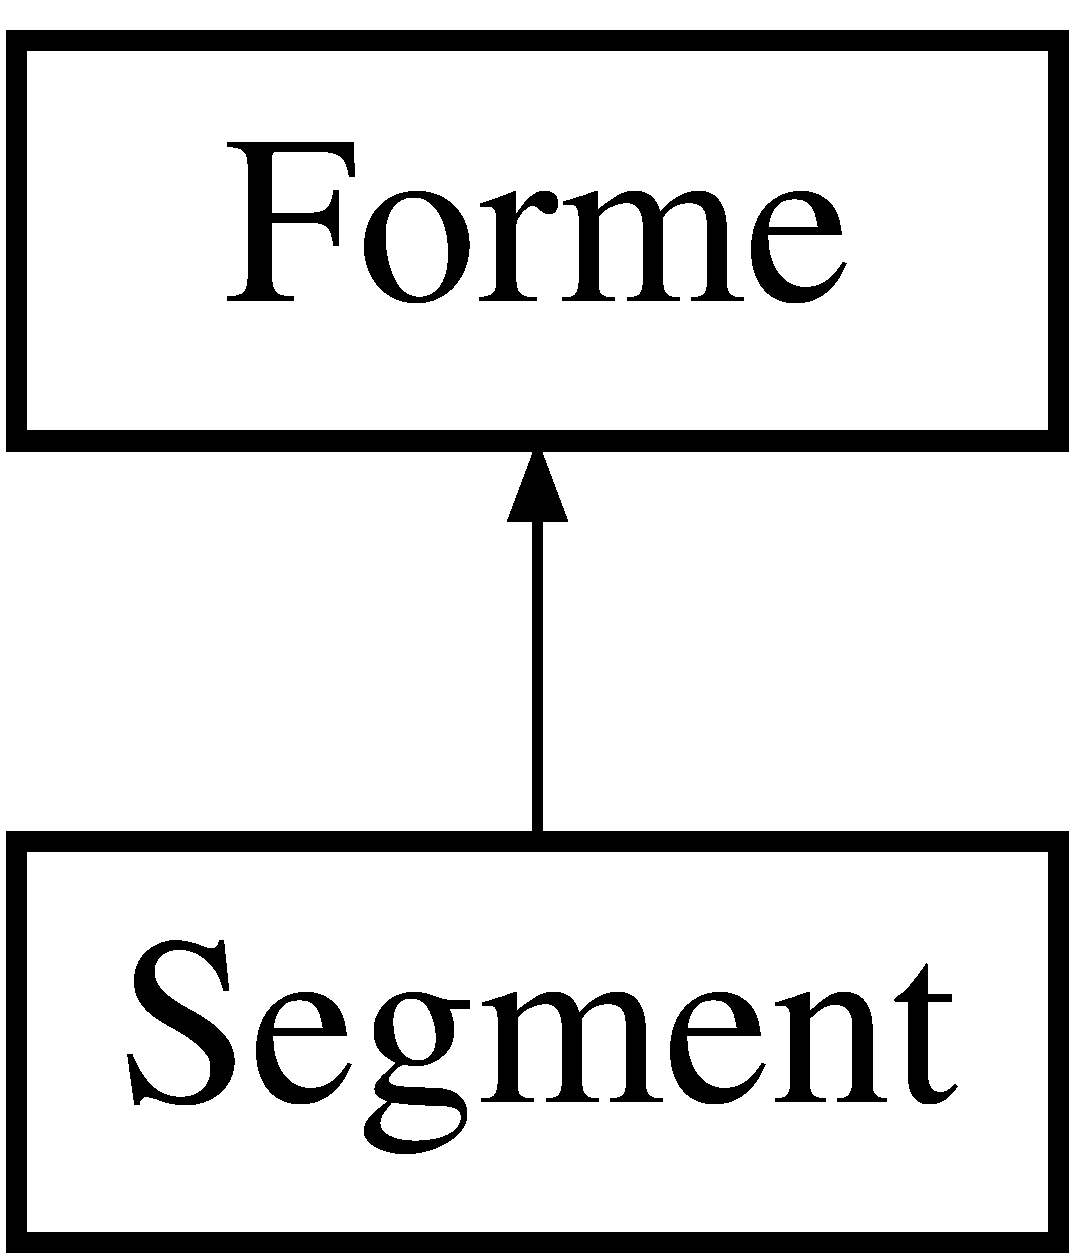
\includegraphics[height=2.000000cm]{class_segment}
\end{center}
\end{figure}
\subsection*{Fonctions membres publiques}
\begin{DoxyCompactItemize}
\item 
\mbox{\hyperlink{class_segment_a8bca782aabb4f612115a5d6db04b9c69}{Segment}} (const \mbox{\hyperlink{class_vecteur2_d}{Vecteur2D}} \&PO, const \mbox{\hyperlink{class_vecteur2_d}{Vecteur2D}} \&PE, const \mbox{\hyperlink{class_couleur}{Couleur}} \&coul=\mbox{\hyperlink{class_couleur}{Couleur}}())
\begin{DoxyCompactList}\small\item\em Constructeur � partir du point d\textquotesingle{}origine et du point de l\textquotesingle{}autre extr�mit� \end{DoxyCompactList}\item 
\mbox{\hyperlink{class_segment_a69e23bf285e63835b6f27a4807162fd0}{Segment}} (const \mbox{\hyperlink{class_segment}{Segment}} \&segment)
\begin{DoxyCompactList}\small\item\em Constructeur par recopie d\textquotesingle{}un segment. \end{DoxyCompactList}\item 
\mbox{\Hypertarget{class_segment_a76b45a453304f1f485e3bc2fcad58b59}\label{class_segment_a76b45a453304f1f485e3bc2fcad58b59}} 
\mbox{\hyperlink{class_segment_a76b45a453304f1f485e3bc2fcad58b59}{$\sim$\+Segment}} ()
\begin{DoxyCompactList}\small\item\em Destructeur. \end{DoxyCompactList}\item 
\mbox{\hyperlink{class_vecteur2_d}{Vecteur2D}} \mbox{\hyperlink{class_segment_ac990ecdbeb9b95fee3b44a38cda9f7ec}{get\+PO}} () const
\begin{DoxyCompactList}\small\item\em Getter pour r�cup�rer le point d\textquotesingle{}origine du segment. \end{DoxyCompactList}\item 
void \mbox{\hyperlink{class_segment_a6ab32e4f1aa7b543df6c5166bfc5bfe2}{set\+PO}} (const \mbox{\hyperlink{class_vecteur2_d}{Vecteur2D}} \&PO)
\begin{DoxyCompactList}\small\item\em Setter pour modifier le point d\textquotesingle{}origine du segment. \end{DoxyCompactList}\item 
\mbox{\hyperlink{class_vecteur2_d}{Vecteur2D}} \mbox{\hyperlink{class_segment_aa1674f72dca782c50d3c19c10e838fe2}{get\+PE}} () const
\begin{DoxyCompactList}\small\item\em Getter pour r�cup�rer le point d\textquotesingle{}extr�mit� du segment. \end{DoxyCompactList}\item 
void \mbox{\hyperlink{class_segment_ac2b5bafebcb80d5ff2f7d5964b17d901}{set\+PE}} (const \mbox{\hyperlink{class_vecteur2_d}{Vecteur2D}} \&PE)
\begin{DoxyCompactList}\small\item\em Setter pour modifier le point d\textquotesingle{}extr�mit� du segment. \end{DoxyCompactList}\item 
\mbox{\Hypertarget{class_segment_a28b3be893a35a0d73574354752c147fd}\label{class_segment_a28b3be893a35a0d73574354752c147fd}} 
\mbox{\hyperlink{class_segment_a28b3be893a35a0d73574354752c147fd}{operator string}} () const
\begin{DoxyCompactList}\small\item\em Surcharge de string pour convertir des segments en string. \end{DoxyCompactList}\item 
bool \mbox{\hyperlink{class_segment_a8bfbc49f9a45d34a52894a75fb81f00a}{operator==}} (const \mbox{\hyperlink{class_segment}{Segment}} \&objet) const
\begin{DoxyCompactList}\small\item\em Surcharge de l\textquotesingle{}op�rateur == pour tester si deux segments sont identiques. \end{DoxyCompactList}\item 
bool \mbox{\hyperlink{class_segment_a9053ffa4a74d85e16db28b151803c7f7}{operator!=}} (const \mbox{\hyperlink{class_segment}{Segment}} \&objet) const
\begin{DoxyCompactList}\small\item\em Surcharge de l\textquotesingle{}op�rateur !=, utilise ==. \end{DoxyCompactList}\item 
const \mbox{\hyperlink{class_segment}{Segment}} \& \mbox{\hyperlink{class_segment_a7f92b771dabbdcbd52f62431a07dbad7}{operator=}} (const \mbox{\hyperlink{class_segment}{Segment}} \&obj)
\begin{DoxyCompactList}\small\item\em Surcharge de l\textquotesingle{}op�rateur =, pour affecter les valeurs d\textquotesingle{}un segment � un autre. \end{DoxyCompactList}\item 
const double \mbox{\hyperlink{class_segment_ab5d7a7584c28a3f306ce9f82b9b71d43}{get\+Aire}} () const
\begin{DoxyCompactList}\small\item\em Getter pour r�cup�rer l\textquotesingle{}aire du segment (toujours = 0) \end{DoxyCompactList}\item 
\mbox{\hyperlink{class_forme}{Forme}} $\ast$ \mbox{\hyperlink{class_segment_a219b06579e425a818933813df8b22232}{clone}} () const
\begin{DoxyCompactList}\small\item\em Clone un segment. \end{DoxyCompactList}\item 
void \mbox{\hyperlink{class_segment_aa71198ab2350e4536a9bdbb0f8179a05}{homothetie}} (const \mbox{\hyperlink{class_vecteur2_d}{Vecteur2D}} \&vect\+Homotethie, double k)
\begin{DoxyCompactList}\small\item\em Effectue une homoth�tie directement sur le segment. \end{DoxyCompactList}\item 
void \mbox{\hyperlink{class_segment_acd838b6258da2a18d1f0f5f76d32b6d1}{translation}} (const \mbox{\hyperlink{class_vecteur2_d}{Vecteur2D}} \&vect\+Translation)
\begin{DoxyCompactList}\small\item\em Effectue une translation directement sur le segment. \end{DoxyCompactList}\item 
void \mbox{\hyperlink{class_segment_a77c334ce9c358ff3dc72b431b380eabe}{rotation}} (const \mbox{\hyperlink{class_vecteur2_d}{Vecteur2D}} \&vect\+Centre, double angle)
\begin{DoxyCompactList}\small\item\em Effectue une rotation directement sur le segment. \end{DoxyCompactList}\item 
ostream \& \mbox{\hyperlink{class_segment_a41e90e3615ca17a67ac0fe0bb3a99223}{print}} (ostream \&flux) const
\begin{DoxyCompactList}\small\item\em Affiche les informations d\textquotesingle{}un segment. \end{DoxyCompactList}\item 
void \mbox{\hyperlink{class_segment_aaad6697e62e1e881ef6aa21a91b6d9ca}{accepte\+Sauvegarder}} (const \mbox{\hyperlink{class_visiteur_sauv_t_x_t}{Visiteur\+Sauv\+T\+XT}} $\ast$v) const
\begin{DoxyCompactList}\small\item\em Appelle la m�thode visite du visiteur de sauvegarde correpondant au segment. \end{DoxyCompactList}\item 
void \mbox{\hyperlink{class_segment_a11de1e065225eb89e7b952a51e918276}{dessiner}} (const \mbox{\hyperlink{class_visiteur_dessin}{Visiteur\+Dessin}} $\ast$v) const
\begin{DoxyCompactList}\small\item\em Appelle la m�thode visite du visiteur de dessin correpondant au segment. \end{DoxyCompactList}\end{DoxyCompactItemize}


\subsection{Documentation des constructeurs et destructeur}
\mbox{\Hypertarget{class_segment_a8bca782aabb4f612115a5d6db04b9c69}\label{class_segment_a8bca782aabb4f612115a5d6db04b9c69}} 
\index{Segment@{Segment}!Segment@{Segment}}
\index{Segment@{Segment}!Segment@{Segment}}
\subsubsection{\texorpdfstring{Segment()}{Segment()}\hspace{0.1cm}{\footnotesize\ttfamily [1/2]}}
{\footnotesize\ttfamily Segment\+::\+Segment (\begin{DoxyParamCaption}\item[{const \mbox{\hyperlink{class_vecteur2_d}{Vecteur2D}} \&}]{PO,  }\item[{const \mbox{\hyperlink{class_vecteur2_d}{Vecteur2D}} \&}]{PE,  }\item[{const \mbox{\hyperlink{class_couleur}{Couleur}} \&}]{coul = {\ttfamily \mbox{\hyperlink{class_couleur}{Couleur}}()} }\end{DoxyParamCaption})}



Constructeur � partir du point d\textquotesingle{}origine et du point de l\textquotesingle{}autre extr�mit� 


\begin{DoxyParams}{Paramètres}
{\em PO} & \mbox{\hyperlink{class_vecteur2_d}{Vecteur2D}} \\
\hline
{\em PE} & vecteur2D \\
\hline
{\em coul} & \mbox{\hyperlink{class_couleur}{Couleur}} par d�faut \\
\hline
\end{DoxyParams}
\mbox{\Hypertarget{class_segment_a69e23bf285e63835b6f27a4807162fd0}\label{class_segment_a69e23bf285e63835b6f27a4807162fd0}} 
\index{Segment@{Segment}!Segment@{Segment}}
\index{Segment@{Segment}!Segment@{Segment}}
\subsubsection{\texorpdfstring{Segment()}{Segment()}\hspace{0.1cm}{\footnotesize\ttfamily [2/2]}}
{\footnotesize\ttfamily Segment\+::\+Segment (\begin{DoxyParamCaption}\item[{const \mbox{\hyperlink{class_segment}{Segment}} \&}]{segment }\end{DoxyParamCaption})}



Constructeur par recopie d\textquotesingle{}un segment. 


\begin{DoxyParams}{Paramètres}
{\em segment} & Le segment � copier \\
\hline
\end{DoxyParams}


\subsection{Documentation des fonctions membres}
\mbox{\Hypertarget{class_segment_aaad6697e62e1e881ef6aa21a91b6d9ca}\label{class_segment_aaad6697e62e1e881ef6aa21a91b6d9ca}} 
\index{Segment@{Segment}!accepteSauvegarder@{accepteSauvegarder}}
\index{accepteSauvegarder@{accepteSauvegarder}!Segment@{Segment}}
\subsubsection{\texorpdfstring{accepteSauvegarder()}{accepteSauvegarder()}}
{\footnotesize\ttfamily void Segment\+::accepte\+Sauvegarder (\begin{DoxyParamCaption}\item[{const \mbox{\hyperlink{class_visiteur_sauv_t_x_t}{Visiteur\+Sauv\+T\+XT}} $\ast$}]{v }\end{DoxyParamCaption}) const\hspace{0.3cm}{\ttfamily [virtual]}}



Appelle la m�thode visite du visiteur de sauvegarde correpondant au segment. 


\begin{DoxyParams}{Paramètres}
{\em v} & Pointeur sur le visiteur de sauvegarde \\
\hline
\end{DoxyParams}


Implémente \mbox{\hyperlink{class_forme_a7be10bca98001dc368adc3a3e93d0f48}{Forme}}.

\mbox{\Hypertarget{class_segment_a219b06579e425a818933813df8b22232}\label{class_segment_a219b06579e425a818933813df8b22232}} 
\index{Segment@{Segment}!clone@{clone}}
\index{clone@{clone}!Segment@{Segment}}
\subsubsection{\texorpdfstring{clone()}{clone()}}
{\footnotesize\ttfamily \mbox{\hyperlink{class_forme}{Forme}} $\ast$ Segment\+::clone (\begin{DoxyParamCaption}{ }\end{DoxyParamCaption}) const\hspace{0.3cm}{\ttfamily [virtual]}}



Clone un segment. 

\begin{DoxyReturn}{Renvoie}
Forme$\ast$ Pointeur sur le segment clon� 
\end{DoxyReturn}


Implémente \mbox{\hyperlink{class_forme_a226750dc3f772514fe58e1dc16f3d0d5}{Forme}}.

\mbox{\Hypertarget{class_segment_a11de1e065225eb89e7b952a51e918276}\label{class_segment_a11de1e065225eb89e7b952a51e918276}} 
\index{Segment@{Segment}!dessiner@{dessiner}}
\index{dessiner@{dessiner}!Segment@{Segment}}
\subsubsection{\texorpdfstring{dessiner()}{dessiner()}}
{\footnotesize\ttfamily void Segment\+::dessiner (\begin{DoxyParamCaption}\item[{const \mbox{\hyperlink{class_visiteur_dessin}{Visiteur\+Dessin}} $\ast$}]{v }\end{DoxyParamCaption}) const\hspace{0.3cm}{\ttfamily [virtual]}}



Appelle la m�thode visite du visiteur de dessin correpondant au segment. 


\begin{DoxyParams}{Paramètres}
{\em v} & Pointeur sur le visiteur de dessin \\
\hline
\end{DoxyParams}


Implémente \mbox{\hyperlink{class_forme_a8cd4879a6a5751cbf6d3bbbfbec41566}{Forme}}.

\mbox{\Hypertarget{class_segment_ab5d7a7584c28a3f306ce9f82b9b71d43}\label{class_segment_ab5d7a7584c28a3f306ce9f82b9b71d43}} 
\index{Segment@{Segment}!getAire@{getAire}}
\index{getAire@{getAire}!Segment@{Segment}}
\subsubsection{\texorpdfstring{getAire()}{getAire()}}
{\footnotesize\ttfamily const double Segment\+::get\+Aire (\begin{DoxyParamCaption}{ }\end{DoxyParamCaption}) const\hspace{0.3cm}{\ttfamily [virtual]}}



Getter pour r�cup�rer l\textquotesingle{}aire du segment (toujours = 0) 

\begin{DoxyReturn}{Renvoie}
R�l Aire du segment (=0) 
\end{DoxyReturn}


Implémente \mbox{\hyperlink{class_forme_adf4346150d8f734d7a48f7661e30cab4}{Forme}}.

\mbox{\Hypertarget{class_segment_aa1674f72dca782c50d3c19c10e838fe2}\label{class_segment_aa1674f72dca782c50d3c19c10e838fe2}} 
\index{Segment@{Segment}!getPE@{getPE}}
\index{getPE@{getPE}!Segment@{Segment}}
\subsubsection{\texorpdfstring{getPE()}{getPE()}}
{\footnotesize\ttfamily \mbox{\hyperlink{class_vecteur2_d}{Vecteur2D}} Segment\+::get\+PE (\begin{DoxyParamCaption}{ }\end{DoxyParamCaption}) const}



Getter pour r�cup�rer le point d\textquotesingle{}extr�mit� du segment. 

\begin{DoxyReturn}{Renvoie}
\mbox{\hyperlink{class_vecteur2_d}{Vecteur2D}} Le point d\textquotesingle{}extr�mit� 
\end{DoxyReturn}
\mbox{\Hypertarget{class_segment_ac990ecdbeb9b95fee3b44a38cda9f7ec}\label{class_segment_ac990ecdbeb9b95fee3b44a38cda9f7ec}} 
\index{Segment@{Segment}!getPO@{getPO}}
\index{getPO@{getPO}!Segment@{Segment}}
\subsubsection{\texorpdfstring{getPO()}{getPO()}}
{\footnotesize\ttfamily \mbox{\hyperlink{class_vecteur2_d}{Vecteur2D}} Segment\+::get\+PO (\begin{DoxyParamCaption}{ }\end{DoxyParamCaption}) const}



Getter pour r�cup�rer le point d\textquotesingle{}origine du segment. 

\begin{DoxyReturn}{Renvoie}
\mbox{\hyperlink{class_vecteur2_d}{Vecteur2D}} Le point d\textquotesingle{}origine 
\end{DoxyReturn}
\mbox{\Hypertarget{class_segment_aa71198ab2350e4536a9bdbb0f8179a05}\label{class_segment_aa71198ab2350e4536a9bdbb0f8179a05}} 
\index{Segment@{Segment}!homothetie@{homothetie}}
\index{homothetie@{homothetie}!Segment@{Segment}}
\subsubsection{\texorpdfstring{homothetie()}{homothetie()}}
{\footnotesize\ttfamily void Segment\+::homothetie (\begin{DoxyParamCaption}\item[{const \mbox{\hyperlink{class_vecteur2_d}{Vecteur2D}} \&}]{vect\+Homotethie,  }\item[{double}]{k }\end{DoxyParamCaption})\hspace{0.3cm}{\ttfamily [virtual]}}



Effectue une homoth�tie directement sur le segment. 


\begin{DoxyParams}{Paramètres}
{\em vect\+Homothetie} & \mbox{\hyperlink{class_vecteur2_d}{Vecteur2D}} \\
\hline
{\em k} & R�el \\
\hline
\end{DoxyParams}


Implémente \mbox{\hyperlink{class_forme_aeaae98ea3de8523de9ba9093e19779d8}{Forme}}.

\mbox{\Hypertarget{class_segment_a9053ffa4a74d85e16db28b151803c7f7}\label{class_segment_a9053ffa4a74d85e16db28b151803c7f7}} 
\index{Segment@{Segment}!operator"!=@{operator"!=}}
\index{operator"!=@{operator"!=}!Segment@{Segment}}
\subsubsection{\texorpdfstring{operator"!=()}{operator!=()}}
{\footnotesize\ttfamily bool Segment\+::operator!= (\begin{DoxyParamCaption}\item[{const \mbox{\hyperlink{class_segment}{Segment}} \&}]{objet }\end{DoxyParamCaption}) const}



Surcharge de l\textquotesingle{}op�rateur !=, utilise ==. 


\begin{DoxyParams}{Paramètres}
{\em objet} & \mbox{\hyperlink{class_segment}{Segment}} � comparer \\
\hline
\end{DoxyParams}
\begin{DoxyReturn}{Renvoie}
bool Bool�en vrai si les deux semgents sont diff�rents, faux sinon 
\end{DoxyReturn}
\mbox{\Hypertarget{class_segment_a7f92b771dabbdcbd52f62431a07dbad7}\label{class_segment_a7f92b771dabbdcbd52f62431a07dbad7}} 
\index{Segment@{Segment}!operator=@{operator=}}
\index{operator=@{operator=}!Segment@{Segment}}
\subsubsection{\texorpdfstring{operator=()}{operator=()}}
{\footnotesize\ttfamily const \mbox{\hyperlink{class_segment}{Segment}} \& Segment\+::operator= (\begin{DoxyParamCaption}\item[{const \mbox{\hyperlink{class_segment}{Segment}} \&}]{obj }\end{DoxyParamCaption})}



Surcharge de l\textquotesingle{}op�rateur =, pour affecter les valeurs d\textquotesingle{}un segment � un autre. 


\begin{DoxyParams}{Paramètres}
{\em obj} & Objet � copier \\
\hline
\end{DoxyParams}
\begin{DoxyReturn}{Renvoie}
\mbox{\hyperlink{class_segment}{Segment}} La resultante de l\textquotesingle{}affectation du segment 
\end{DoxyReturn}
\mbox{\Hypertarget{class_segment_a8bfbc49f9a45d34a52894a75fb81f00a}\label{class_segment_a8bfbc49f9a45d34a52894a75fb81f00a}} 
\index{Segment@{Segment}!operator==@{operator==}}
\index{operator==@{operator==}!Segment@{Segment}}
\subsubsection{\texorpdfstring{operator==()}{operator==()}}
{\footnotesize\ttfamily bool Segment\+::operator== (\begin{DoxyParamCaption}\item[{const \mbox{\hyperlink{class_segment}{Segment}} \&}]{objet }\end{DoxyParamCaption}) const}



Surcharge de l\textquotesingle{}op�rateur == pour tester si deux segments sont identiques. 


\begin{DoxyParams}{Paramètres}
{\em objet} & \mbox{\hyperlink{class_segment}{Segment}} � comparer \\
\hline
\end{DoxyParams}
\begin{DoxyReturn}{Renvoie}
bool Bool�en vrai si les deux segments sont identiques, faux sinon 
\end{DoxyReturn}
\mbox{\Hypertarget{class_segment_a41e90e3615ca17a67ac0fe0bb3a99223}\label{class_segment_a41e90e3615ca17a67ac0fe0bb3a99223}} 
\index{Segment@{Segment}!print@{print}}
\index{print@{print}!Segment@{Segment}}
\subsubsection{\texorpdfstring{print()}{print()}}
{\footnotesize\ttfamily ostream \& Segment\+::print (\begin{DoxyParamCaption}\item[{ostream \&}]{flux }\end{DoxyParamCaption}) const\hspace{0.3cm}{\ttfamily [virtual]}}



Affiche les informations d\textquotesingle{}un segment. 


\begin{DoxyParams}{Paramètres}
{\em flux} & Flux de sortie \\
\hline
\end{DoxyParams}
\begin{DoxyReturn}{Renvoie}
ostream Flux de sortie 
\end{DoxyReturn}


Réimplémentée à partir de \mbox{\hyperlink{class_forme_a348a12ae03fe2167ffd586f4deae6c76}{Forme}}.

\mbox{\Hypertarget{class_segment_a77c334ce9c358ff3dc72b431b380eabe}\label{class_segment_a77c334ce9c358ff3dc72b431b380eabe}} 
\index{Segment@{Segment}!rotation@{rotation}}
\index{rotation@{rotation}!Segment@{Segment}}
\subsubsection{\texorpdfstring{rotation()}{rotation()}}
{\footnotesize\ttfamily void Segment\+::rotation (\begin{DoxyParamCaption}\item[{const \mbox{\hyperlink{class_vecteur2_d}{Vecteur2D}} \&}]{vect\+Centre,  }\item[{double}]{angle }\end{DoxyParamCaption})\hspace{0.3cm}{\ttfamily [virtual]}}



Effectue une rotation directement sur le segment. 


\begin{DoxyParams}{Paramètres}
{\em vect\+Translation} & \mbox{\hyperlink{class_vecteur2_d}{Vecteur2D}} \\
\hline
{\em angle} & R�el \\
\hline
\end{DoxyParams}


Implémente \mbox{\hyperlink{class_forme_af17c4156d00281b4b62d8c27dcb75569}{Forme}}.

\mbox{\Hypertarget{class_segment_ac2b5bafebcb80d5ff2f7d5964b17d901}\label{class_segment_ac2b5bafebcb80d5ff2f7d5964b17d901}} 
\index{Segment@{Segment}!setPE@{setPE}}
\index{setPE@{setPE}!Segment@{Segment}}
\subsubsection{\texorpdfstring{setPE()}{setPE()}}
{\footnotesize\ttfamily void Segment\+::set\+PE (\begin{DoxyParamCaption}\item[{const \mbox{\hyperlink{class_vecteur2_d}{Vecteur2D}} \&}]{PE }\end{DoxyParamCaption})}



Setter pour modifier le point d\textquotesingle{}extr�mit� du segment. 


\begin{DoxyParams}{Paramètres}
{\em PE} & \mbox{\hyperlink{class_vecteur2_d}{Vecteur2D}} \\
\hline
\end{DoxyParams}
\mbox{\Hypertarget{class_segment_a6ab32e4f1aa7b543df6c5166bfc5bfe2}\label{class_segment_a6ab32e4f1aa7b543df6c5166bfc5bfe2}} 
\index{Segment@{Segment}!setPO@{setPO}}
\index{setPO@{setPO}!Segment@{Segment}}
\subsubsection{\texorpdfstring{setPO()}{setPO()}}
{\footnotesize\ttfamily void Segment\+::set\+PO (\begin{DoxyParamCaption}\item[{const \mbox{\hyperlink{class_vecteur2_d}{Vecteur2D}} \&}]{PO }\end{DoxyParamCaption})}



Setter pour modifier le point d\textquotesingle{}origine du segment. 


\begin{DoxyParams}{Paramètres}
{\em PO} & \mbox{\hyperlink{class_vecteur2_d}{Vecteur2D}} \\
\hline
\end{DoxyParams}
\mbox{\Hypertarget{class_segment_acd838b6258da2a18d1f0f5f76d32b6d1}\label{class_segment_acd838b6258da2a18d1f0f5f76d32b6d1}} 
\index{Segment@{Segment}!translation@{translation}}
\index{translation@{translation}!Segment@{Segment}}
\subsubsection{\texorpdfstring{translation()}{translation()}}
{\footnotesize\ttfamily void Segment\+::translation (\begin{DoxyParamCaption}\item[{const \mbox{\hyperlink{class_vecteur2_d}{Vecteur2D}} \&}]{vect\+Translation }\end{DoxyParamCaption})\hspace{0.3cm}{\ttfamily [virtual]}}



Effectue une translation directement sur le segment. 


\begin{DoxyParams}{Paramètres}
{\em vect\+Translation} & \mbox{\hyperlink{class_vecteur2_d}{Vecteur2D}} \\
\hline
\end{DoxyParams}


Implémente \mbox{\hyperlink{class_forme_ad156a02098ef453b09919b2a3156f607}{Forme}}.



La documentation de cette classe a été générée à partir des fichiers suivants \+:\begin{DoxyCompactItemize}
\item 
\mbox{\hyperlink{_segment_8h}{Segment.\+h}}\item 
Segment.\+cpp\end{DoxyCompactItemize}

\hypertarget{class_singleton_connexion}{}\section{Singleton\+Connexion Class Reference}
\label{class_singleton_connexion}\index{Singleton\+Connexion@{Singleton\+Connexion}}


{\ttfamily \#include $<$Singleton\+Connexion.\+h$>$}

\subsection*{Public Member Functions}
\begin{DoxyCompactItemize}
\item 
bool \hyperlink{class_singleton_connexion_ad050c458fa21b5292d982b8ca265fec0}{initialiser\+Connexion} ()
\begin{DoxyCompactList}\small\item\em Initialise la connexion vers le serveur. \end{DoxyCompactList}\item 
void \hyperlink{class_singleton_connexion_a700b93e730b6d57f0c249153420dd12b}{fermer\+Connexion} ()
\begin{DoxyCompactList}\small\item\em Ferme la connexion vers le serveur. \end{DoxyCompactList}\item 
void \hyperlink{class_singleton_connexion_adf9e4f1c58e72f1b4bd3ed9821356c41}{envoyer\+Requete} (const string \&str)
\begin{DoxyCompactList}\small\item\em Envoie une requ�te au serveur. \end{DoxyCompactList}\item 
bool \hyperlink{class_singleton_connexion_a68501656107c8ab123f8ad386731fec9}{serveur\+A\+Traite\+Requete} ()
\begin{DoxyCompactList}\small\item\em Teste si une requ�te a �t� trait�e par le serveur. \end{DoxyCompactList}\end{DoxyCompactItemize}
\subsection*{Static Public Member Functions}
\begin{DoxyCompactItemize}
\item 
static \hyperlink{class_singleton_connexion}{Singleton\+Connexion} $\ast$ \hyperlink{class_singleton_connexion_a58810d15c0a686c4695e1b2373319ab8}{get\+Instance} ()
\begin{DoxyCompactList}\small\item\em Retourne une instance unique. \end{DoxyCompactList}\item 
static void \hyperlink{class_singleton_connexion_a185cc5359c9b2e62a47315d0a3cf311c}{kill\+Instance} ()
\begin{DoxyCompactList}\small\item\em Ferme l\textquotesingle{}instance unique en cours. \end{DoxyCompactList}\end{DoxyCompactItemize}


\subsection{Member Function Documentation}
\mbox{\Hypertarget{class_singleton_connexion_adf9e4f1c58e72f1b4bd3ed9821356c41}\label{class_singleton_connexion_adf9e4f1c58e72f1b4bd3ed9821356c41}} 
\index{Singleton\+Connexion@{Singleton\+Connexion}!envoyer\+Requete@{envoyer\+Requete}}
\index{envoyer\+Requete@{envoyer\+Requete}!Singleton\+Connexion@{Singleton\+Connexion}}
\subsubsection{\texorpdfstring{envoyer\+Requete()}{envoyerRequete()}}
{\footnotesize\ttfamily void Singleton\+Connexion\+::envoyer\+Requete (\begin{DoxyParamCaption}\item[{const string \&}]{str }\end{DoxyParamCaption})}



Envoie une requ�te au serveur. 


\begin{DoxyParams}{Parameters}
{\em str} & La chaine de caract�re � envoyer au serveur \\
\hline
\end{DoxyParams}
\mbox{\Hypertarget{class_singleton_connexion_a700b93e730b6d57f0c249153420dd12b}\label{class_singleton_connexion_a700b93e730b6d57f0c249153420dd12b}} 
\index{Singleton\+Connexion@{Singleton\+Connexion}!fermer\+Connexion@{fermer\+Connexion}}
\index{fermer\+Connexion@{fermer\+Connexion}!Singleton\+Connexion@{Singleton\+Connexion}}
\subsubsection{\texorpdfstring{fermer\+Connexion()}{fermerConnexion()}}
{\footnotesize\ttfamily void Singleton\+Connexion\+::fermer\+Connexion (\begin{DoxyParamCaption}{ }\end{DoxyParamCaption})}



Ferme la connexion vers le serveur. 

\mbox{\Hypertarget{class_singleton_connexion_a58810d15c0a686c4695e1b2373319ab8}\label{class_singleton_connexion_a58810d15c0a686c4695e1b2373319ab8}} 
\index{Singleton\+Connexion@{Singleton\+Connexion}!get\+Instance@{get\+Instance}}
\index{get\+Instance@{get\+Instance}!Singleton\+Connexion@{Singleton\+Connexion}}
\subsubsection{\texorpdfstring{get\+Instance()}{getInstance()}}
{\footnotesize\ttfamily \hyperlink{class_singleton_connexion}{Singleton\+Connexion} $\ast$ Singleton\+Connexion\+::get\+Instance (\begin{DoxyParamCaption}{ }\end{DoxyParamCaption})\hspace{0.3cm}{\ttfamily [static]}}



Retourne une instance unique. 

Va cr�er l\textquotesingle{}instance si celle-\/ci n\textquotesingle{}existe pas ou bien juste la retourner dans le cas contraire \begin{DoxyReturn}{Returns}
Singleton\+Connexion$\ast$ Pointeur sur l\textquotesingle{}instance unique 
\end{DoxyReturn}
\mbox{\Hypertarget{class_singleton_connexion_ad050c458fa21b5292d982b8ca265fec0}\label{class_singleton_connexion_ad050c458fa21b5292d982b8ca265fec0}} 
\index{Singleton\+Connexion@{Singleton\+Connexion}!initialiser\+Connexion@{initialiser\+Connexion}}
\index{initialiser\+Connexion@{initialiser\+Connexion}!Singleton\+Connexion@{Singleton\+Connexion}}
\subsubsection{\texorpdfstring{initialiser\+Connexion()}{initialiserConnexion()}}
{\footnotesize\ttfamily bool Singleton\+Connexion\+::initialiser\+Connexion (\begin{DoxyParamCaption}{ }\end{DoxyParamCaption})}



Initialise la connexion vers le serveur. 

\begin{DoxyReturn}{Returns}
bool Bool�en vrai si la connexion est r�ussie, faux sinon 
\end{DoxyReturn}
\mbox{\Hypertarget{class_singleton_connexion_a185cc5359c9b2e62a47315d0a3cf311c}\label{class_singleton_connexion_a185cc5359c9b2e62a47315d0a3cf311c}} 
\index{Singleton\+Connexion@{Singleton\+Connexion}!kill\+Instance@{kill\+Instance}}
\index{kill\+Instance@{kill\+Instance}!Singleton\+Connexion@{Singleton\+Connexion}}
\subsubsection{\texorpdfstring{kill\+Instance()}{killInstance()}}
{\footnotesize\ttfamily void Singleton\+Connexion\+::kill\+Instance (\begin{DoxyParamCaption}{ }\end{DoxyParamCaption})\hspace{0.3cm}{\ttfamily [static]}}



Ferme l\textquotesingle{}instance unique en cours. 

\mbox{\Hypertarget{class_singleton_connexion_a68501656107c8ab123f8ad386731fec9}\label{class_singleton_connexion_a68501656107c8ab123f8ad386731fec9}} 
\index{Singleton\+Connexion@{Singleton\+Connexion}!serveur\+A\+Traite\+Requete@{serveur\+A\+Traite\+Requete}}
\index{serveur\+A\+Traite\+Requete@{serveur\+A\+Traite\+Requete}!Singleton\+Connexion@{Singleton\+Connexion}}
\subsubsection{\texorpdfstring{serveur\+A\+Traite\+Requete()}{serveurATraiteRequete()}}
{\footnotesize\ttfamily bool Singleton\+Connexion\+::serveur\+A\+Traite\+Requete (\begin{DoxyParamCaption}{ }\end{DoxyParamCaption})}



Teste si une requ�te a �t� trait�e par le serveur. 

\begin{DoxyReturn}{Returns}
bool Bool�en vrai si la requ�te a �t� trait�e, faux sinon 
\end{DoxyReturn}


The documentation for this class was generated from the following files\+:\begin{DoxyCompactItemize}
\item 
C\+:/\+Users/\+Quentin Fixe/\+Desktop/\+P\+P\+I\+L-\/master/\+C\+L\+I\+E\+N\+T/\hyperlink{_singleton_connexion_8h}{Singleton\+Connexion.\+h}\item 
C\+:/\+Users/\+Quentin Fixe/\+Desktop/\+P\+P\+I\+L-\/master/\+C\+L\+I\+E\+N\+T/\hyperlink{_singleton_connexion_8cpp}{Singleton\+Connexion.\+cpp}\end{DoxyCompactItemize}

\hypertarget{class_triangle}{}\section{Triangle Class Reference}
\label{class_triangle}\index{Triangle@{Triangle}}


{\ttfamily \#include $<$Triangle.\+h$>$}

Inheritance diagram for Triangle\+:\begin{figure}[H]
\begin{center}
\leavevmode
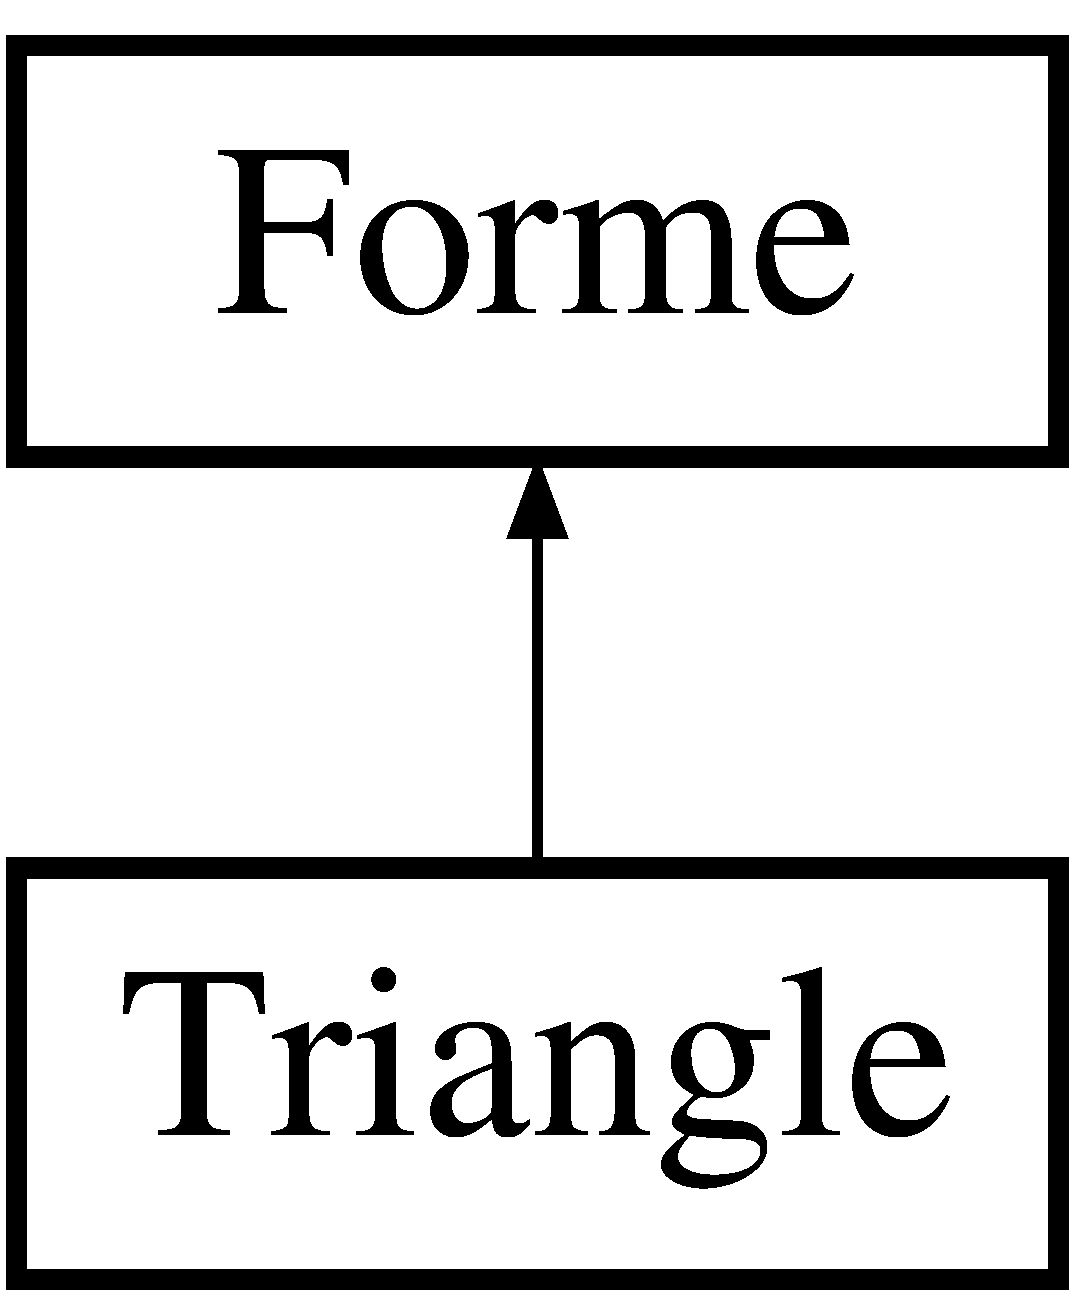
\includegraphics[height=2.000000cm]{class_triangle}
\end{center}
\end{figure}
\subsection*{Public Member Functions}
\begin{DoxyCompactItemize}
\item 
\hyperlink{class_triangle_ab6bdfe32c0c93b3c99cc7cd6739a31a9}{Triangle} (const \hyperlink{class_vecteur2_d}{Vecteur2D} \&P1, const \hyperlink{class_vecteur2_d}{Vecteur2D} \&P2, const \hyperlink{class_vecteur2_d}{Vecteur2D} \&P3, const \hyperlink{class_couleur}{Couleur} \&coul=\hyperlink{class_couleur}{Couleur}())
\begin{DoxyCompactList}\small\item\em Constructeur � partir des 3 points et d\textquotesingle{}une couleur par d�faut. \end{DoxyCompactList}\item 
\hyperlink{class_triangle_a6bf47183caad44f0fb0146a20868e91e}{Triangle} (const \hyperlink{class_triangle}{Triangle} \&\hyperlink{class_triangle}{Triangle})
\begin{DoxyCompactList}\small\item\em Constructeur par recopie d\textquotesingle{}un triangle. \end{DoxyCompactList}\item 
\hyperlink{class_triangle_a5199760a17454f4dc94c855a57e3a152}{$\sim$\+Triangle} ()
\begin{DoxyCompactList}\small\item\em Destructeur. \end{DoxyCompactList}\item 
bool \hyperlink{class_triangle_aaa608eaa59738f8194ab6c0fee8b7f0e}{verif\+Points} (const \hyperlink{class_vecteur2_d}{Vecteur2D} \&P1, const \hyperlink{class_vecteur2_d}{Vecteur2D} \&P2, const \hyperlink{class_vecteur2_d}{Vecteur2D} \&P3)
\begin{DoxyCompactList}\small\item\em V�rifie si les 3 points sont correctement plac�s \end{DoxyCompactList}\item 
\hyperlink{class_vecteur2_d}{Vecteur2D} \hyperlink{class_triangle_a99912480c94bb7776c6fa6cd46424c8c}{get\+P1} () const
\begin{DoxyCompactList}\small\item\em Getter du premier point du triangle. \end{DoxyCompactList}\item 
void \hyperlink{class_triangle_adb012503dca929384bd5a14eb77c817e}{set\+P1} (const \hyperlink{class_vecteur2_d}{Vecteur2D} \&P1)
\begin{DoxyCompactList}\small\item\em Setter du premier point du triangle. \end{DoxyCompactList}\item 
\hyperlink{class_vecteur2_d}{Vecteur2D} \hyperlink{class_triangle_a59c178dc55ee22df0f4742b433686be1}{get\+P2} () const
\begin{DoxyCompactList}\small\item\em Getter du deuxi�me point du triangle. \end{DoxyCompactList}\item 
void \hyperlink{class_triangle_aa449658f51930f7029c93a2316465451}{set\+P2} (const \hyperlink{class_vecteur2_d}{Vecteur2D} \&P2)
\begin{DoxyCompactList}\small\item\em Setter du premier point du triangle. \end{DoxyCompactList}\item 
\hyperlink{class_vecteur2_d}{Vecteur2D} \hyperlink{class_triangle_ae52413a60c37dbc6b017fb484a09c38f}{get\+P3} () const
\begin{DoxyCompactList}\small\item\em Getter du troisi�me point du triangle. \end{DoxyCompactList}\item 
void \hyperlink{class_triangle_ab3567045e50185c07710b9f1669755b2}{set\+P3} (const \hyperlink{class_vecteur2_d}{Vecteur2D} \&P3)
\begin{DoxyCompactList}\small\item\em Setter du troisi�me point du triangle. \end{DoxyCompactList}\item 
\hyperlink{class_triangle_acd8612cc20ffb71e543944c869e4ab81}{operator string} () const
\begin{DoxyCompactList}\small\item\em Surcharge de l\textquotesingle{}op�rateur string qui permet de convertir un \hyperlink{class_triangle}{Triangle} en string. \end{DoxyCompactList}\item 
bool \hyperlink{class_triangle_a9def3caaa3fdcab079ff0c16fef39904}{operator==} (const \hyperlink{class_triangle}{Triangle} \&objet) const
\begin{DoxyCompactList}\small\item\em Surcharge de l\textquotesingle{}op�rateur == qui permet de tester si deux triangles sont identiques. \end{DoxyCompactList}\item 
bool \hyperlink{class_triangle_a6ab1734a5a2f5696363ad24c6910e35c}{operator!=} (const \hyperlink{class_triangle}{Triangle} \&objet) const
\begin{DoxyCompactList}\small\item\em Surcharge de l\textquotesingle{}op�rateur !=, qui utilise ==. \end{DoxyCompactList}\item 
const \hyperlink{class_triangle}{Triangle} \& \hyperlink{class_triangle_a288d9febf55fef68c7e2cf7709f2590d}{operator=} (const \hyperlink{class_triangle}{Triangle} \&obj)
\begin{DoxyCompactList}\small\item\em Surcharge de l\textquotesingle{}op�rateur = qui permet d\textquotesingle{}affecter les valeur d\textquotesingle{}un triangle � un autre. \end{DoxyCompactList}\item 
const double \hyperlink{class_triangle_aa6693ea9778fad637f7b1c73a305c220}{get\+Aire} () const
\begin{DoxyCompactList}\small\item\em Getter pour r�cup�rer l\textquotesingle{}aire du triangle. \end{DoxyCompactList}\item 
\hyperlink{class_forme}{Forme} $\ast$ \hyperlink{class_triangle_a610a6de862fd2f720036ae515dd71930}{clone} () const
\begin{DoxyCompactList}\small\item\em Clone un triangle. \end{DoxyCompactList}\item 
void \hyperlink{class_triangle_a2c15a4513cf35c9275b237ec70bf6df2}{homothetie} (const \hyperlink{class_vecteur2_d}{Vecteur2D} \&vect\+Homotethie, double k)
\begin{DoxyCompactList}\small\item\em Effectue une homot�thie directement sur le triangle. \end{DoxyCompactList}\item 
void \hyperlink{class_triangle_aa1b2a542395e4e8c67f35757159c4d4b}{translation} (const \hyperlink{class_vecteur2_d}{Vecteur2D} \&vect\+Translation)
\begin{DoxyCompactList}\small\item\em Effectue une translation directement sur le triangle. \end{DoxyCompactList}\item 
void \hyperlink{class_triangle_a6e728d1e72366e42b2afbf1e13b6d8f7}{rotation} (const \hyperlink{class_vecteur2_d}{Vecteur2D} \&vect\+Centre, double angle)
\begin{DoxyCompactList}\small\item\em Effectue une rotation directement sur le triangle. \end{DoxyCompactList}\item 
ostream \& \hyperlink{class_triangle_a9e810bfe4577a2e590235d5388cbee03}{print} (ostream \&flux) const
\begin{DoxyCompactList}\small\item\em Affiche les informations concernant un triangle. \end{DoxyCompactList}\item 
void \hyperlink{class_triangle_af0ad5baa5cd45c0a1afd40690ebed849}{accepte\+Sauvegarder} (const \hyperlink{class_visiteur_sauv_t_x_t}{Visiteur\+Sauv\+T\+XT} $\ast$v) const
\begin{DoxyCompactList}\small\item\em Appelle la m�thode visite du visiteur de sauvegarde correpondant au triangle. \end{DoxyCompactList}\item 
void \hyperlink{class_triangle_af4d344ab356b33b90a095022adc42434}{dessiner} (const \hyperlink{class_visiteur_dessin}{Visiteur\+Dessin} $\ast$v) const
\begin{DoxyCompactList}\small\item\em Appelle la m�thode visite du visiteur de dessin correpondant au triangle. \end{DoxyCompactList}\end{DoxyCompactItemize}


\subsection{Constructor \& Destructor Documentation}
\mbox{\Hypertarget{class_triangle_ab6bdfe32c0c93b3c99cc7cd6739a31a9}\label{class_triangle_ab6bdfe32c0c93b3c99cc7cd6739a31a9}} 
\index{Triangle@{Triangle}!Triangle@{Triangle}}
\index{Triangle@{Triangle}!Triangle@{Triangle}}
\subsubsection{\texorpdfstring{Triangle()}{Triangle()}\hspace{0.1cm}{\footnotesize\ttfamily [1/2]}}
{\footnotesize\ttfamily Triangle\+::\+Triangle (\begin{DoxyParamCaption}\item[{const \hyperlink{class_vecteur2_d}{Vecteur2D} \&}]{P1,  }\item[{const \hyperlink{class_vecteur2_d}{Vecteur2D} \&}]{P2,  }\item[{const \hyperlink{class_vecteur2_d}{Vecteur2D} \&}]{P3,  }\item[{const \hyperlink{class_couleur}{Couleur} \&}]{coul = {\ttfamily \hyperlink{class_couleur}{Couleur}()} }\end{DoxyParamCaption})}



Constructeur � partir des 3 points et d\textquotesingle{}une couleur par d�faut. 


\begin{DoxyParams}{Parameters}
{\em P1} & \hyperlink{class_vecteur2_d}{Vecteur2D} \\
\hline
{\em P2} & \hyperlink{class_vecteur2_d}{Vecteur2D} \\
\hline
{\em P3} & \hyperlink{class_vecteur2_d}{Vecteur2D} \\
\hline
\end{DoxyParams}
\mbox{\Hypertarget{class_triangle_a6bf47183caad44f0fb0146a20868e91e}\label{class_triangle_a6bf47183caad44f0fb0146a20868e91e}} 
\index{Triangle@{Triangle}!Triangle@{Triangle}}
\index{Triangle@{Triangle}!Triangle@{Triangle}}
\subsubsection{\texorpdfstring{Triangle()}{Triangle()}\hspace{0.1cm}{\footnotesize\ttfamily [2/2]}}
{\footnotesize\ttfamily Triangle\+::\+Triangle (\begin{DoxyParamCaption}\item[{const \hyperlink{class_triangle}{Triangle} \&}]{Triangle }\end{DoxyParamCaption})}



Constructeur par recopie d\textquotesingle{}un triangle. 


\begin{DoxyParams}{Parameters}
{\em \hyperlink{class_triangle}{Triangle}} & \hyperlink{class_triangle}{Triangle} � recopier \\
\hline
\end{DoxyParams}
\mbox{\Hypertarget{class_triangle_a5199760a17454f4dc94c855a57e3a152}\label{class_triangle_a5199760a17454f4dc94c855a57e3a152}} 
\index{Triangle@{Triangle}!````~Triangle@{$\sim$\+Triangle}}
\index{````~Triangle@{$\sim$\+Triangle}!Triangle@{Triangle}}
\subsubsection{\texorpdfstring{$\sim$\+Triangle()}{~Triangle()}}
{\footnotesize\ttfamily Triangle\+::$\sim$\+Triangle (\begin{DoxyParamCaption}{ }\end{DoxyParamCaption})}



Destructeur. 



\subsection{Member Function Documentation}
\mbox{\Hypertarget{class_triangle_af0ad5baa5cd45c0a1afd40690ebed849}\label{class_triangle_af0ad5baa5cd45c0a1afd40690ebed849}} 
\index{Triangle@{Triangle}!accepte\+Sauvegarder@{accepte\+Sauvegarder}}
\index{accepte\+Sauvegarder@{accepte\+Sauvegarder}!Triangle@{Triangle}}
\subsubsection{\texorpdfstring{accepte\+Sauvegarder()}{accepteSauvegarder()}}
{\footnotesize\ttfamily void Triangle\+::accepte\+Sauvegarder (\begin{DoxyParamCaption}\item[{const \hyperlink{class_visiteur_sauv_t_x_t}{Visiteur\+Sauv\+T\+XT} $\ast$}]{v }\end{DoxyParamCaption}) const\hspace{0.3cm}{\ttfamily [virtual]}}



Appelle la m�thode visite du visiteur de sauvegarde correpondant au triangle. 


\begin{DoxyParams}{Parameters}
{\em v} & Pointeur sur le visiteur de sauvegarde \\
\hline
\end{DoxyParams}


Implements \hyperlink{class_forme_a7be10bca98001dc368adc3a3e93d0f48}{Forme}.

\mbox{\Hypertarget{class_triangle_a610a6de862fd2f720036ae515dd71930}\label{class_triangle_a610a6de862fd2f720036ae515dd71930}} 
\index{Triangle@{Triangle}!clone@{clone}}
\index{clone@{clone}!Triangle@{Triangle}}
\subsubsection{\texorpdfstring{clone()}{clone()}}
{\footnotesize\ttfamily \hyperlink{class_forme}{Forme} $\ast$ Triangle\+::clone (\begin{DoxyParamCaption}{ }\end{DoxyParamCaption}) const\hspace{0.3cm}{\ttfamily [virtual]}}



Clone un triangle. 

\begin{DoxyReturn}{Returns}
Forme$\ast$ Un pointeur sur le triangle clon� 
\end{DoxyReturn}


Implements \hyperlink{class_forme_a226750dc3f772514fe58e1dc16f3d0d5}{Forme}.

\mbox{\Hypertarget{class_triangle_af4d344ab356b33b90a095022adc42434}\label{class_triangle_af4d344ab356b33b90a095022adc42434}} 
\index{Triangle@{Triangle}!dessiner@{dessiner}}
\index{dessiner@{dessiner}!Triangle@{Triangle}}
\subsubsection{\texorpdfstring{dessiner()}{dessiner()}}
{\footnotesize\ttfamily void Triangle\+::dessiner (\begin{DoxyParamCaption}\item[{const \hyperlink{class_visiteur_dessin}{Visiteur\+Dessin} $\ast$}]{v }\end{DoxyParamCaption}) const\hspace{0.3cm}{\ttfamily [virtual]}}



Appelle la m�thode visite du visiteur de dessin correpondant au triangle. 


\begin{DoxyParams}{Parameters}
{\em v} & Pointeur sur le visiteur de dessin \\
\hline
\end{DoxyParams}


Implements \hyperlink{class_forme_a8cd4879a6a5751cbf6d3bbbfbec41566}{Forme}.

\mbox{\Hypertarget{class_triangle_aa6693ea9778fad637f7b1c73a305c220}\label{class_triangle_aa6693ea9778fad637f7b1c73a305c220}} 
\index{Triangle@{Triangle}!get\+Aire@{get\+Aire}}
\index{get\+Aire@{get\+Aire}!Triangle@{Triangle}}
\subsubsection{\texorpdfstring{get\+Aire()}{getAire()}}
{\footnotesize\ttfamily const double Triangle\+::get\+Aire (\begin{DoxyParamCaption}{ }\end{DoxyParamCaption}) const\hspace{0.3cm}{\ttfamily [virtual]}}



Getter pour r�cup�rer l\textquotesingle{}aire du triangle. 

\begin{DoxyReturn}{Returns}
R�el L\textquotesingle{}aire du triangle 
\end{DoxyReturn}


Implements \hyperlink{class_forme_adf4346150d8f734d7a48f7661e30cab4}{Forme}.

\mbox{\Hypertarget{class_triangle_a99912480c94bb7776c6fa6cd46424c8c}\label{class_triangle_a99912480c94bb7776c6fa6cd46424c8c}} 
\index{Triangle@{Triangle}!get\+P1@{get\+P1}}
\index{get\+P1@{get\+P1}!Triangle@{Triangle}}
\subsubsection{\texorpdfstring{get\+P1()}{getP1()}}
{\footnotesize\ttfamily \hyperlink{class_vecteur2_d}{Vecteur2D} Triangle\+::get\+P1 (\begin{DoxyParamCaption}{ }\end{DoxyParamCaption}) const}



Getter du premier point du triangle. 

\begin{DoxyReturn}{Returns}
\hyperlink{class_vecteur2_d}{Vecteur2D} Le premier point du triangle 
\end{DoxyReturn}
\mbox{\Hypertarget{class_triangle_a59c178dc55ee22df0f4742b433686be1}\label{class_triangle_a59c178dc55ee22df0f4742b433686be1}} 
\index{Triangle@{Triangle}!get\+P2@{get\+P2}}
\index{get\+P2@{get\+P2}!Triangle@{Triangle}}
\subsubsection{\texorpdfstring{get\+P2()}{getP2()}}
{\footnotesize\ttfamily \hyperlink{class_vecteur2_d}{Vecteur2D} Triangle\+::get\+P2 (\begin{DoxyParamCaption}{ }\end{DoxyParamCaption}) const}



Getter du deuxi�me point du triangle. 

\begin{DoxyReturn}{Returns}
\hyperlink{class_vecteur2_d}{Vecteur2D} Le deuxi�me point du triangle 
\end{DoxyReturn}
\mbox{\Hypertarget{class_triangle_ae52413a60c37dbc6b017fb484a09c38f}\label{class_triangle_ae52413a60c37dbc6b017fb484a09c38f}} 
\index{Triangle@{Triangle}!get\+P3@{get\+P3}}
\index{get\+P3@{get\+P3}!Triangle@{Triangle}}
\subsubsection{\texorpdfstring{get\+P3()}{getP3()}}
{\footnotesize\ttfamily \hyperlink{class_vecteur2_d}{Vecteur2D} Triangle\+::get\+P3 (\begin{DoxyParamCaption}{ }\end{DoxyParamCaption}) const}



Getter du troisi�me point du triangle. 

\begin{DoxyReturn}{Returns}
\hyperlink{class_vecteur2_d}{Vecteur2D} Le troisi�me point du triangle 
\end{DoxyReturn}
\mbox{\Hypertarget{class_triangle_a2c15a4513cf35c9275b237ec70bf6df2}\label{class_triangle_a2c15a4513cf35c9275b237ec70bf6df2}} 
\index{Triangle@{Triangle}!homothetie@{homothetie}}
\index{homothetie@{homothetie}!Triangle@{Triangle}}
\subsubsection{\texorpdfstring{homothetie()}{homothetie()}}
{\footnotesize\ttfamily void Triangle\+::homothetie (\begin{DoxyParamCaption}\item[{const \hyperlink{class_vecteur2_d}{Vecteur2D} \&}]{vect\+Homotethie,  }\item[{double}]{k }\end{DoxyParamCaption})\hspace{0.3cm}{\ttfamily [virtual]}}



Effectue une homot�thie directement sur le triangle. 


\begin{DoxyParams}{Parameters}
{\em vect\+Homoth�tie} & \hyperlink{class_vecteur2_d}{Vecteur2D} \\
\hline
{\em k} & R�el \\
\hline
\end{DoxyParams}


Implements \hyperlink{class_forme_aeaae98ea3de8523de9ba9093e19779d8}{Forme}.

\mbox{\Hypertarget{class_triangle_acd8612cc20ffb71e543944c869e4ab81}\label{class_triangle_acd8612cc20ffb71e543944c869e4ab81}} 
\index{Triangle@{Triangle}!operator string@{operator string}}
\index{operator string@{operator string}!Triangle@{Triangle}}
\subsubsection{\texorpdfstring{operator string()}{operator string()}}
{\footnotesize\ttfamily Triangle\+::operator string (\begin{DoxyParamCaption}{ }\end{DoxyParamCaption}) const\hspace{0.3cm}{\ttfamily [virtual]}}



Surcharge de l\textquotesingle{}op�rateur string qui permet de convertir un \hyperlink{class_triangle}{Triangle} en string. 



Reimplemented from \hyperlink{class_forme_a809375f023f0f19227f3e3821ee56731}{Forme}.

\mbox{\Hypertarget{class_triangle_a6ab1734a5a2f5696363ad24c6910e35c}\label{class_triangle_a6ab1734a5a2f5696363ad24c6910e35c}} 
\index{Triangle@{Triangle}!operator"!=@{operator"!=}}
\index{operator"!=@{operator"!=}!Triangle@{Triangle}}
\subsubsection{\texorpdfstring{operator"!=()}{operator!=()}}
{\footnotesize\ttfamily bool Triangle\+::operator!= (\begin{DoxyParamCaption}\item[{const \hyperlink{class_triangle}{Triangle} \&}]{objet }\end{DoxyParamCaption}) const}



Surcharge de l\textquotesingle{}op�rateur !=, qui utilise ==. 


\begin{DoxyParams}{Parameters}
{\em objet} & Le triangle � comparer \\
\hline
\end{DoxyParams}
\begin{DoxyReturn}{Returns}
Bool�en vrai si les deux triangles sont diff�rents, faux sinon 
\end{DoxyReturn}
\mbox{\Hypertarget{class_triangle_a288d9febf55fef68c7e2cf7709f2590d}\label{class_triangle_a288d9febf55fef68c7e2cf7709f2590d}} 
\index{Triangle@{Triangle}!operator=@{operator=}}
\index{operator=@{operator=}!Triangle@{Triangle}}
\subsubsection{\texorpdfstring{operator=()}{operator=()}}
{\footnotesize\ttfamily const \hyperlink{class_triangle}{Triangle} \& Triangle\+::operator= (\begin{DoxyParamCaption}\item[{const \hyperlink{class_triangle}{Triangle} \&}]{obj }\end{DoxyParamCaption})}



Surcharge de l\textquotesingle{}op�rateur = qui permet d\textquotesingle{}affecter les valeur d\textquotesingle{}un triangle � un autre. 


\begin{DoxyParams}{Parameters}
{\em obj} & \hyperlink{class_triangle}{Triangle} � affecter \\
\hline
\end{DoxyParams}
\begin{DoxyReturn}{Returns}
\hyperlink{class_triangle}{Triangle} affect� par les nouvelles valeurs 
\end{DoxyReturn}
\mbox{\Hypertarget{class_triangle_a9def3caaa3fdcab079ff0c16fef39904}\label{class_triangle_a9def3caaa3fdcab079ff0c16fef39904}} 
\index{Triangle@{Triangle}!operator==@{operator==}}
\index{operator==@{operator==}!Triangle@{Triangle}}
\subsubsection{\texorpdfstring{operator==()}{operator==()}}
{\footnotesize\ttfamily bool Triangle\+::operator== (\begin{DoxyParamCaption}\item[{const \hyperlink{class_triangle}{Triangle} \&}]{objet }\end{DoxyParamCaption}) const}



Surcharge de l\textquotesingle{}op�rateur == qui permet de tester si deux triangles sont identiques. 


\begin{DoxyParams}{Parameters}
{\em objet} & \hyperlink{class_triangle}{Triangle} � comparer \\
\hline
\end{DoxyParams}
\begin{DoxyReturn}{Returns}
bool Bool�en vrai si les deux triangles sont identiques, faux sinon 
\end{DoxyReturn}
\mbox{\Hypertarget{class_triangle_a9e810bfe4577a2e590235d5388cbee03}\label{class_triangle_a9e810bfe4577a2e590235d5388cbee03}} 
\index{Triangle@{Triangle}!print@{print}}
\index{print@{print}!Triangle@{Triangle}}
\subsubsection{\texorpdfstring{print()}{print()}}
{\footnotesize\ttfamily ostream \& Triangle\+::print (\begin{DoxyParamCaption}\item[{ostream \&}]{flux }\end{DoxyParamCaption}) const\hspace{0.3cm}{\ttfamily [virtual]}}



Affiche les informations concernant un triangle. 


\begin{DoxyParams}{Parameters}
{\em flux} & Le flux sortant \\
\hline
\end{DoxyParams}
\begin{DoxyReturn}{Returns}
ostream Flux sortant 
\end{DoxyReturn}


Reimplemented from \hyperlink{class_forme_a348a12ae03fe2167ffd586f4deae6c76}{Forme}.

\mbox{\Hypertarget{class_triangle_a6e728d1e72366e42b2afbf1e13b6d8f7}\label{class_triangle_a6e728d1e72366e42b2afbf1e13b6d8f7}} 
\index{Triangle@{Triangle}!rotation@{rotation}}
\index{rotation@{rotation}!Triangle@{Triangle}}
\subsubsection{\texorpdfstring{rotation()}{rotation()}}
{\footnotesize\ttfamily void Triangle\+::rotation (\begin{DoxyParamCaption}\item[{const \hyperlink{class_vecteur2_d}{Vecteur2D} \&}]{vect\+Centre,  }\item[{double}]{angle }\end{DoxyParamCaption})\hspace{0.3cm}{\ttfamily [virtual]}}



Effectue une rotation directement sur le triangle. 


\begin{DoxyParams}{Parameters}
{\em vect\+Centre} & \hyperlink{class_vecteur2_d}{Vecteur2D} \\
\hline
{\em angle} & R�el \\
\hline
\end{DoxyParams}


Implements \hyperlink{class_forme_af17c4156d00281b4b62d8c27dcb75569}{Forme}.

\mbox{\Hypertarget{class_triangle_adb012503dca929384bd5a14eb77c817e}\label{class_triangle_adb012503dca929384bd5a14eb77c817e}} 
\index{Triangle@{Triangle}!set\+P1@{set\+P1}}
\index{set\+P1@{set\+P1}!Triangle@{Triangle}}
\subsubsection{\texorpdfstring{set\+P1()}{setP1()}}
{\footnotesize\ttfamily void Triangle\+::set\+P1 (\begin{DoxyParamCaption}\item[{const \hyperlink{class_vecteur2_d}{Vecteur2D} \&}]{P1 }\end{DoxyParamCaption})}



Setter du premier point du triangle. 


\begin{DoxyParams}{Parameters}
{\em P1} & \hyperlink{class_vecteur2_d}{Vecteur2D} \\
\hline
\end{DoxyParams}
\mbox{\Hypertarget{class_triangle_aa449658f51930f7029c93a2316465451}\label{class_triangle_aa449658f51930f7029c93a2316465451}} 
\index{Triangle@{Triangle}!set\+P2@{set\+P2}}
\index{set\+P2@{set\+P2}!Triangle@{Triangle}}
\subsubsection{\texorpdfstring{set\+P2()}{setP2()}}
{\footnotesize\ttfamily void Triangle\+::set\+P2 (\begin{DoxyParamCaption}\item[{const \hyperlink{class_vecteur2_d}{Vecteur2D} \&}]{P2 }\end{DoxyParamCaption})}



Setter du premier point du triangle. 


\begin{DoxyParams}{Parameters}
{\em P2} & vecteur2D \\
\hline
\end{DoxyParams}
\mbox{\Hypertarget{class_triangle_ab3567045e50185c07710b9f1669755b2}\label{class_triangle_ab3567045e50185c07710b9f1669755b2}} 
\index{Triangle@{Triangle}!set\+P3@{set\+P3}}
\index{set\+P3@{set\+P3}!Triangle@{Triangle}}
\subsubsection{\texorpdfstring{set\+P3()}{setP3()}}
{\footnotesize\ttfamily void Triangle\+::set\+P3 (\begin{DoxyParamCaption}\item[{const \hyperlink{class_vecteur2_d}{Vecteur2D} \&}]{P3 }\end{DoxyParamCaption})}



Setter du troisi�me point du triangle. 


\begin{DoxyParams}{Parameters}
{\em P3} & \hyperlink{class_vecteur2_d}{Vecteur2D} \\
\hline
\end{DoxyParams}
\mbox{\Hypertarget{class_triangle_aa1b2a542395e4e8c67f35757159c4d4b}\label{class_triangle_aa1b2a542395e4e8c67f35757159c4d4b}} 
\index{Triangle@{Triangle}!translation@{translation}}
\index{translation@{translation}!Triangle@{Triangle}}
\subsubsection{\texorpdfstring{translation()}{translation()}}
{\footnotesize\ttfamily void Triangle\+::translation (\begin{DoxyParamCaption}\item[{const \hyperlink{class_vecteur2_d}{Vecteur2D} \&}]{vect\+Translation }\end{DoxyParamCaption})\hspace{0.3cm}{\ttfamily [virtual]}}



Effectue une translation directement sur le triangle. 


\begin{DoxyParams}{Parameters}
{\em vect\+Translation} & \hyperlink{class_vecteur2_d}{Vecteur2D} \\
\hline
\end{DoxyParams}


Implements \hyperlink{class_forme_ad156a02098ef453b09919b2a3156f607}{Forme}.

\mbox{\Hypertarget{class_triangle_aaa608eaa59738f8194ab6c0fee8b7f0e}\label{class_triangle_aaa608eaa59738f8194ab6c0fee8b7f0e}} 
\index{Triangle@{Triangle}!verif\+Points@{verif\+Points}}
\index{verif\+Points@{verif\+Points}!Triangle@{Triangle}}
\subsubsection{\texorpdfstring{verif\+Points()}{verifPoints()}}
{\footnotesize\ttfamily bool Triangle\+::verif\+Points (\begin{DoxyParamCaption}\item[{const \hyperlink{class_vecteur2_d}{Vecteur2D} \&}]{P1,  }\item[{const \hyperlink{class_vecteur2_d}{Vecteur2D} \&}]{P2,  }\item[{const \hyperlink{class_vecteur2_d}{Vecteur2D} \&}]{P3 }\end{DoxyParamCaption})}



V�rifie si les 3 points sont correctement plac�s 


\begin{DoxyParams}{Parameters}
{\em P1} & \hyperlink{class_vecteur2_d}{Vecteur2D} \\
\hline
{\em P2} & vecteur2D \\
\hline
{\em P3} & \hyperlink{class_vecteur2_d}{Vecteur2D} \\
\hline
\end{DoxyParams}
\begin{DoxyReturn}{Returns}
bool Bool�en vrai si les points sont bien plac�s, faux sinon 
\end{DoxyReturn}


The documentation for this class was generated from the following files\+:\begin{DoxyCompactItemize}
\item 
C\+:/\+Users/\+Quentin Fixe/\+Desktop/\+P\+P\+I\+L-\/master/\+C\+L\+I\+E\+N\+T/\hyperlink{_triangle_8h}{Triangle.\+h}\item 
C\+:/\+Users/\+Quentin Fixe/\+Desktop/\+P\+P\+I\+L-\/master/\+C\+L\+I\+E\+N\+T/\hyperlink{_triangle_8cpp}{Triangle.\+cpp}\end{DoxyCompactItemize}

\hypertarget{class_vecteur2_d}{}\section{Référence de la classe Vecteur2D}
\label{class_vecteur2_d}\index{Vecteur2D@{Vecteur2D}}
\subsection*{Fonctions membres publiques}
\begin{DoxyCompactItemize}
\item 
\mbox{\hyperlink{class_vecteur2_d_ad9dee29de356e9bd4bee597dddf431b0}{Vecteur2D}} (const double \&x=0, const double \&y=0)
\begin{DoxyCompactList}\small\item\em Constructeur � partir des coordonn�es x et y. \end{DoxyCompactList}\item 
\mbox{\hyperlink{class_vecteur2_d_ad27a38b26a6b5e17b1a7643999eb1947}{Vecteur2D}} (const \mbox{\hyperlink{class_vecteur2_d}{Vecteur2D}} \&v)
\begin{DoxyCompactList}\small\item\em Constructeur par copie � partir d\textquotesingle{}un vecteur. \end{DoxyCompactList}\item 
\mbox{\Hypertarget{class_vecteur2_d_aa7a40ecd8c31e20ad910c4ae0be2fe56}\label{class_vecteur2_d_aa7a40ecd8c31e20ad910c4ae0be2fe56}} 
virtual \mbox{\hyperlink{class_vecteur2_d_aa7a40ecd8c31e20ad910c4ae0be2fe56}{$\sim$\+Vecteur2D}} ()
\begin{DoxyCompactList}\small\item\em Destructeur. \end{DoxyCompactList}\item 
const double \mbox{\hyperlink{class_vecteur2_d_a7f4eb5a1c2a7c44f3b4821bdff2d2a75}{getX}} () const
\begin{DoxyCompactList}\small\item\em Getter de l\textquotesingle{}attribut priv� x. \end{DoxyCompactList}\item 
void \mbox{\hyperlink{class_vecteur2_d_a6f34b3f3278d1784ab4a30e9d549346c}{setX}} (const double \&x)
\begin{DoxyCompactList}\small\item\em Setter de l\textquotesingle{}attribut priv� x. \end{DoxyCompactList}\item 
const double \mbox{\hyperlink{class_vecteur2_d_a9765748bf73ae58a67af8edd3ec46cc2}{getY}} () const
\begin{DoxyCompactList}\small\item\em Getter de l\textquotesingle{}attribut y. \end{DoxyCompactList}\item 
void \mbox{\hyperlink{class_vecteur2_d_abd64918f46162b331929cde3102388b2}{setY}} (const double \&y)
\begin{DoxyCompactList}\small\item\em Setter de l\textquotesingle{}attribut y. \end{DoxyCompactList}\item 
const \mbox{\hyperlink{class_vecteur2_d}{Vecteur2D}} \mbox{\hyperlink{class_vecteur2_d_aaed6615f626d64f66d77e17dfdb8c2f0}{operator+}} (const \mbox{\hyperlink{class_vecteur2_d}{Vecteur2D}} \&u) const
\item 
const \mbox{\hyperlink{class_vecteur2_d}{Vecteur2D}} \mbox{\hyperlink{class_vecteur2_d_aaca13009f4c8bd1d4707e80a0ba83380}{operator $\ast$}} (const double \&a) const
\begin{DoxyCompactList}\small\item\em Op�rateur de multiplication par un facteur a. \end{DoxyCompactList}\item 
const \mbox{\hyperlink{class_vecteur2_d}{Vecteur2D}} \mbox{\hyperlink{class_vecteur2_d_ad66f16f464a7c1b7a92cff4d8414b9d6}{operator -\/}} () const
\begin{DoxyCompactList}\small\item\em Op�rateur de soustraction (surcharg� ici comme oppos� d\textquotesingle{}un vecteur) \end{DoxyCompactList}\item 
bool \mbox{\hyperlink{class_vecteur2_d_ab98bdc37a2de06a3ce50243515c2c71e}{operator==}} (const \mbox{\hyperlink{class_vecteur2_d}{Vecteur2D}} \&objet) const
\begin{DoxyCompactList}\small\item\em Test d\textquotesingle{}�galit� avec un autre vecteur. \end{DoxyCompactList}\item 
bool \mbox{\hyperlink{class_vecteur2_d_ad55d80402cf0cd4cce5b1a6f11ec77fc}{operator !=}} (const \mbox{\hyperlink{class_vecteur2_d}{Vecteur2D}} \&v) const
\item 
const \mbox{\hyperlink{class_vecteur2_d}{Vecteur2D}} \mbox{\hyperlink{class_vecteur2_d_a60b85acf37779913dfe6ca1a00ea1648}{operator=}} (const \mbox{\hyperlink{class_vecteur2_d}{Vecteur2D}} \&objet)
\begin{DoxyCompactList}\small\item\em Op�rateur d\textquotesingle{}affectation. \end{DoxyCompactList}\item 
\mbox{\hyperlink{class_vecteur2_d_a10c83f5b0aaa60cc01912b33e3c76fc5}{operator string}} () const
\begin{DoxyCompactList}\small\item\em Operateur de conversion \mbox{\hyperlink{class_vecteur2_d}{Vecteur2D}} en string. \end{DoxyCompactList}\item 
void \mbox{\hyperlink{class_vecteur2_d_a7e7340ad14aac6c6155ba57829629696}{homothetie}} (const \mbox{\hyperlink{class_vecteur2_d}{Vecteur2D}} \&point\+Invariant, double k)
\begin{DoxyCompactList}\small\item\em Une homoth�tie est d�finie par un point invariant et un rapport de grandeurs vectorielles constant (k) qui modifie directement le vecteur. \end{DoxyCompactList}\item 
void \mbox{\hyperlink{class_vecteur2_d_a32e581bbc22cd5a7a6e2d4d5ec54d41b}{translation}} (const \mbox{\hyperlink{class_vecteur2_d}{Vecteur2D}} \&vect\+Translation)
\begin{DoxyCompactList}\small\item\em Une translation est d�finie par un vecteur de translation qui modifie directement le vecteur. \end{DoxyCompactList}\item 
void \mbox{\hyperlink{class_vecteur2_d_a0246a048cea97398ea9c98d090ccaf9e}{rotation}} (const \mbox{\hyperlink{class_vecteur2_d}{Vecteur2D}} \&vect\+Centre, double angle)
\begin{DoxyCompactList}\small\item\em Une rotation est d�finie par un point invariant (le centre de la rotation) et par un angle sign� donn� en radians. Modifie directement le vecteur. \end{DoxyCompactList}\item 
const double \mbox{\hyperlink{class_vecteur2_d_a8f1f65f3efaeab323d9487373612282b}{determinant}} (const \mbox{\hyperlink{class_vecteur2_d}{Vecteur2D}} \&v) const
\begin{DoxyCompactList}\small\item\em Calcul du d�terminant(u , v), ici le d�terminant r�pr�sente l\textquotesingle{}aire du parall�logramme form� par u et v. \end{DoxyCompactList}\end{DoxyCompactItemize}
\subsection*{Amis}
\begin{DoxyCompactItemize}
\item 
ostream \& \mbox{\hyperlink{class_vecteur2_d_a62103e3ee59519a5bc33e0bdc0728699}{operator$<$$<$}} (ostream \&os, const \mbox{\hyperlink{class_vecteur2_d}{Vecteur2D}} \&u)
\begin{DoxyCompactList}\small\item\em Surcharge l\textquotesingle{}affichage dans un flux de sortie. \end{DoxyCompactList}\end{DoxyCompactItemize}


\subsection{Documentation des constructeurs et destructeur}
\mbox{\Hypertarget{class_vecteur2_d_ad9dee29de356e9bd4bee597dddf431b0}\label{class_vecteur2_d_ad9dee29de356e9bd4bee597dddf431b0}} 
\index{Vecteur2D@{Vecteur2D}!Vecteur2D@{Vecteur2D}}
\index{Vecteur2D@{Vecteur2D}!Vecteur2D@{Vecteur2D}}
\subsubsection{\texorpdfstring{Vecteur2D()}{Vecteur2D()}\hspace{0.1cm}{\footnotesize\ttfamily [1/2]}}
{\footnotesize\ttfamily Vecteur2\+D\+::\+Vecteur2D (\begin{DoxyParamCaption}\item[{const double \&}]{x = {\ttfamily 0},  }\item[{const double \&}]{y = {\ttfamily 0} }\end{DoxyParamCaption})\hspace{0.3cm}{\ttfamily [explicit]}}



Constructeur � partir des coordonn�es x et y. 

Les coordonn�es x et y sont par d�faut mis � 0. 
\begin{DoxyParams}{Paramètres}
{\em x} & R�el \\
\hline
{\em y} & R�el \\
\hline
\end{DoxyParams}
\mbox{\Hypertarget{class_vecteur2_d_ad27a38b26a6b5e17b1a7643999eb1947}\label{class_vecteur2_d_ad27a38b26a6b5e17b1a7643999eb1947}} 
\index{Vecteur2D@{Vecteur2D}!Vecteur2D@{Vecteur2D}}
\index{Vecteur2D@{Vecteur2D}!Vecteur2D@{Vecteur2D}}
\subsubsection{\texorpdfstring{Vecteur2D()}{Vecteur2D()}\hspace{0.1cm}{\footnotesize\ttfamily [2/2]}}
{\footnotesize\ttfamily Vecteur2\+D\+::\+Vecteur2D (\begin{DoxyParamCaption}\item[{const \mbox{\hyperlink{class_vecteur2_d}{Vecteur2D}} \&}]{v }\end{DoxyParamCaption})}



Constructeur par copie � partir d\textquotesingle{}un vecteur. 

Recopie les coordonn�es du vecteur pass� en param�tre dans {\itshape x} et {\itshape y}. 
\begin{DoxyParams}{Paramètres}
{\em v} & Vecteur de points \\
\hline
\end{DoxyParams}


\subsection{Documentation des fonctions membres}
\mbox{\Hypertarget{class_vecteur2_d_a8f1f65f3efaeab323d9487373612282b}\label{class_vecteur2_d_a8f1f65f3efaeab323d9487373612282b}} 
\index{Vecteur2D@{Vecteur2D}!determinant@{determinant}}
\index{determinant@{determinant}!Vecteur2D@{Vecteur2D}}
\subsubsection{\texorpdfstring{determinant()}{determinant()}}
{\footnotesize\ttfamily const double Vecteur2\+D\+::determinant (\begin{DoxyParamCaption}\item[{const \mbox{\hyperlink{class_vecteur2_d}{Vecteur2D}} \&}]{v }\end{DoxyParamCaption}) const}



Calcul du d�terminant(u , v), ici le d�terminant r�pr�sente l\textquotesingle{}aire du parall�logramme form� par u et v. 


\begin{DoxyParams}{Paramètres}
{\em v} & \mbox{\hyperlink{class_vecteur2_d}{Vecteur2D}}. \\
\hline
\end{DoxyParams}
\begin{DoxyReturn}{Renvoie}
Un R�el r�sultat de det(u, v). 
\end{DoxyReturn}
\mbox{\Hypertarget{class_vecteur2_d_a7f4eb5a1c2a7c44f3b4821bdff2d2a75}\label{class_vecteur2_d_a7f4eb5a1c2a7c44f3b4821bdff2d2a75}} 
\index{Vecteur2D@{Vecteur2D}!getX@{getX}}
\index{getX@{getX}!Vecteur2D@{Vecteur2D}}
\subsubsection{\texorpdfstring{getX()}{getX()}}
{\footnotesize\ttfamily const double Vecteur2\+D\+::getX (\begin{DoxyParamCaption}{ }\end{DoxyParamCaption}) const}



Getter de l\textquotesingle{}attribut priv� x. 

\begin{DoxyReturn}{Renvoie}
Un r�el \+: l\textquotesingle{}abcisse stock�e dans l\textquotesingle{}attribut priv� x 
\end{DoxyReturn}
\mbox{\Hypertarget{class_vecteur2_d_a9765748bf73ae58a67af8edd3ec46cc2}\label{class_vecteur2_d_a9765748bf73ae58a67af8edd3ec46cc2}} 
\index{Vecteur2D@{Vecteur2D}!getY@{getY}}
\index{getY@{getY}!Vecteur2D@{Vecteur2D}}
\subsubsection{\texorpdfstring{getY()}{getY()}}
{\footnotesize\ttfamily const double Vecteur2\+D\+::getY (\begin{DoxyParamCaption}{ }\end{DoxyParamCaption}) const}



Getter de l\textquotesingle{}attribut y. 

\begin{DoxyReturn}{Renvoie}
Un r�el \+: l\textquotesingle{}ordonn�e stock�e dans l\textquotesingle{}attribut y. 
\end{DoxyReturn}
\mbox{\Hypertarget{class_vecteur2_d_a7e7340ad14aac6c6155ba57829629696}\label{class_vecteur2_d_a7e7340ad14aac6c6155ba57829629696}} 
\index{Vecteur2D@{Vecteur2D}!homothetie@{homothetie}}
\index{homothetie@{homothetie}!Vecteur2D@{Vecteur2D}}
\subsubsection{\texorpdfstring{homothetie()}{homothetie()}}
{\footnotesize\ttfamily void Vecteur2\+D\+::homothetie (\begin{DoxyParamCaption}\item[{const \mbox{\hyperlink{class_vecteur2_d}{Vecteur2D}} \&}]{point\+Invariant,  }\item[{double}]{k }\end{DoxyParamCaption})}



Une homoth�tie est d�finie par un point invariant et un rapport de grandeurs vectorielles constant (k) qui modifie directement le vecteur. 


\begin{DoxyParams}{Paramètres}
{\em point\+Invariant} & \mbox{\hyperlink{class_vecteur2_d}{Vecteur2D}}, k R�el \\
\hline
\end{DoxyParams}
\mbox{\Hypertarget{class_vecteur2_d_ad55d80402cf0cd4cce5b1a6f11ec77fc}\label{class_vecteur2_d_ad55d80402cf0cd4cce5b1a6f11ec77fc}} 
\index{Vecteur2D@{Vecteur2D}!operator "!=@{operator "!=}}
\index{operator "!=@{operator "!=}!Vecteur2D@{Vecteur2D}}
\subsubsection{\texorpdfstring{operator "!=()}{operator !=()}}
{\footnotesize\ttfamily bool Vecteur2\+D\+::operator != (\begin{DoxyParamCaption}\item[{const \mbox{\hyperlink{class_vecteur2_d}{Vecteur2D}} \&}]{v }\end{DoxyParamCaption}) const}

\textbackslash{} brief Test de diff�rence avec un autre vecteur.

Utilise l\textquotesingle{}op�rateur d\textquotesingle{}�galit�. 
\begin{DoxyParams}{Paramètres}
{\em objet} & \mbox{\hyperlink{class_vecteur2_d}{Vecteur2D}} \\
\hline
\end{DoxyParams}
\begin{DoxyReturn}{Renvoie}
Un bool�en true si in�galit� et false sinon. 
\end{DoxyReturn}
\mbox{\Hypertarget{class_vecteur2_d_aaca13009f4c8bd1d4707e80a0ba83380}\label{class_vecteur2_d_aaca13009f4c8bd1d4707e80a0ba83380}} 
\index{Vecteur2D@{Vecteur2D}!operator $\ast$@{operator $\ast$}}
\index{operator $\ast$@{operator $\ast$}!Vecteur2D@{Vecteur2D}}
\subsubsection{\texorpdfstring{operator $\ast$()}{operator *()}}
{\footnotesize\ttfamily const \mbox{\hyperlink{class_vecteur2_d}{Vecteur2D}} Vecteur2\+D\+::operator $\ast$ (\begin{DoxyParamCaption}\item[{const double \&}]{a }\end{DoxyParamCaption}) const}



Op�rateur de multiplication par un facteur a. 


\begin{DoxyParams}{Paramètres}
{\em a} & R�el \\
\hline
\end{DoxyParams}
\begin{DoxyReturn}{Renvoie}
\mbox{\hyperlink{class_vecteur2_d}{Vecteur2D}} Une copie du r�sultat de l\textquotesingle{}op�ration 
\end{DoxyReturn}
\mbox{\Hypertarget{class_vecteur2_d_ad66f16f464a7c1b7a92cff4d8414b9d6}\label{class_vecteur2_d_ad66f16f464a7c1b7a92cff4d8414b9d6}} 
\index{Vecteur2D@{Vecteur2D}!operator -\/@{operator -\/}}
\index{operator -\/@{operator -\/}!Vecteur2D@{Vecteur2D}}
\subsubsection{\texorpdfstring{operator -\/()}{operator -()}}
{\footnotesize\ttfamily const \mbox{\hyperlink{class_vecteur2_d}{Vecteur2D}} Vecteur2\+D\+::operator -\/ (\begin{DoxyParamCaption}{ }\end{DoxyParamCaption}) const}



Op�rateur de soustraction (surcharg� ici comme oppos� d\textquotesingle{}un vecteur) 

\begin{DoxyReturn}{Renvoie}
\mbox{\hyperlink{class_vecteur2_d}{Vecteur2D}} Une copie du r�sultat de l\textquotesingle{}op�ration 
\end{DoxyReturn}
\mbox{\Hypertarget{class_vecteur2_d_a10c83f5b0aaa60cc01912b33e3c76fc5}\label{class_vecteur2_d_a10c83f5b0aaa60cc01912b33e3c76fc5}} 
\index{Vecteur2D@{Vecteur2D}!operator string@{operator string}}
\index{operator string@{operator string}!Vecteur2D@{Vecteur2D}}
\subsubsection{\texorpdfstring{operator string()}{operator string()}}
{\footnotesize\ttfamily Vecteur2\+D\+::operator string (\begin{DoxyParamCaption}{ }\end{DoxyParamCaption}) const}



Operateur de conversion \mbox{\hyperlink{class_vecteur2_d}{Vecteur2D}} en string. 

Conversion des coordonn�es du vecteur en chaines de caract�res. \mbox{\Hypertarget{class_vecteur2_d_aaed6615f626d64f66d77e17dfdb8c2f0}\label{class_vecteur2_d_aaed6615f626d64f66d77e17dfdb8c2f0}} 
\index{Vecteur2D@{Vecteur2D}!operator+@{operator+}}
\index{operator+@{operator+}!Vecteur2D@{Vecteur2D}}
\subsubsection{\texorpdfstring{operator+()}{operator+()}}
{\footnotesize\ttfamily const \mbox{\hyperlink{class_vecteur2_d}{Vecteur2D}} Vecteur2\+D\+::operator+ (\begin{DoxyParamCaption}\item[{const \mbox{\hyperlink{class_vecteur2_d}{Vecteur2D}} \&}]{u }\end{DoxyParamCaption}) const}

\textbackslash{} brief Op�rateur d\textquotesingle{}addition entre deux vecteurs. 
\begin{DoxyParams}{Paramètres}
{\em u} & \mbox{\hyperlink{class_vecteur2_d}{Vecteur2D}} \\
\hline
\end{DoxyParams}
\begin{DoxyReturn}{Renvoie}
\mbox{\hyperlink{class_vecteur2_d}{Vecteur2D}} Une copie du r�sultat de l\textquotesingle{}op�ration 
\end{DoxyReturn}
\mbox{\Hypertarget{class_vecteur2_d_a60b85acf37779913dfe6ca1a00ea1648}\label{class_vecteur2_d_a60b85acf37779913dfe6ca1a00ea1648}} 
\index{Vecteur2D@{Vecteur2D}!operator=@{operator=}}
\index{operator=@{operator=}!Vecteur2D@{Vecteur2D}}
\subsubsection{\texorpdfstring{operator=()}{operator=()}}
{\footnotesize\ttfamily const \mbox{\hyperlink{class_vecteur2_d}{Vecteur2D}} Vecteur2\+D\+::operator= (\begin{DoxyParamCaption}\item[{const \mbox{\hyperlink{class_vecteur2_d}{Vecteur2D}} \&}]{objet }\end{DoxyParamCaption})}



Op�rateur d\textquotesingle{}affectation. 

Modifie les attributs x et y en fonction du \mbox{\hyperlink{class_vecteur2_d}{Vecteur2D}} pass� en param�tre. 
\begin{DoxyParams}{Paramètres}
{\em objet} & \mbox{\hyperlink{class_vecteur2_d}{Vecteur2D}} \\
\hline
\end{DoxyParams}
\begin{DoxyReturn}{Renvoie}
{\itshape \mbox{\hyperlink{class_vecteur2_d}{Vecteur2D}}} r�sultat de l\textquotesingle{}affectaion. 
\end{DoxyReturn}
\mbox{\Hypertarget{class_vecteur2_d_ab98bdc37a2de06a3ce50243515c2c71e}\label{class_vecteur2_d_ab98bdc37a2de06a3ce50243515c2c71e}} 
\index{Vecteur2D@{Vecteur2D}!operator==@{operator==}}
\index{operator==@{operator==}!Vecteur2D@{Vecteur2D}}
\subsubsection{\texorpdfstring{operator==()}{operator==()}}
{\footnotesize\ttfamily bool Vecteur2\+D\+::operator== (\begin{DoxyParamCaption}\item[{const \mbox{\hyperlink{class_vecteur2_d}{Vecteur2D}} \&}]{objet }\end{DoxyParamCaption}) const}



Test d\textquotesingle{}�galit� avec un autre vecteur. 

Compare champ � champ les deux vecteurs. 
\begin{DoxyParams}{Paramètres}
{\em objet} & \mbox{\hyperlink{class_vecteur2_d}{Vecteur2D}} \\
\hline
\end{DoxyParams}
\begin{DoxyReturn}{Renvoie}
Un bool�en true si �galit� et false sinon. 
\end{DoxyReturn}
\mbox{\Hypertarget{class_vecteur2_d_a0246a048cea97398ea9c98d090ccaf9e}\label{class_vecteur2_d_a0246a048cea97398ea9c98d090ccaf9e}} 
\index{Vecteur2D@{Vecteur2D}!rotation@{rotation}}
\index{rotation@{rotation}!Vecteur2D@{Vecteur2D}}
\subsubsection{\texorpdfstring{rotation()}{rotation()}}
{\footnotesize\ttfamily void Vecteur2\+D\+::rotation (\begin{DoxyParamCaption}\item[{const \mbox{\hyperlink{class_vecteur2_d}{Vecteur2D}} \&}]{vect\+Centre,  }\item[{double}]{angle }\end{DoxyParamCaption})}



Une rotation est d�finie par un point invariant (le centre de la rotation) et par un angle sign� donn� en radians. Modifie directement le vecteur. 


\begin{DoxyParams}{Paramètres}
{\em vect\+Centre} & \mbox{\hyperlink{class_vecteur2_d}{Vecteur2D}}, angle R�el. \\
\hline
\end{DoxyParams}
\mbox{\Hypertarget{class_vecteur2_d_a6f34b3f3278d1784ab4a30e9d549346c}\label{class_vecteur2_d_a6f34b3f3278d1784ab4a30e9d549346c}} 
\index{Vecteur2D@{Vecteur2D}!setX@{setX}}
\index{setX@{setX}!Vecteur2D@{Vecteur2D}}
\subsubsection{\texorpdfstring{setX()}{setX()}}
{\footnotesize\ttfamily void Vecteur2\+D\+::setX (\begin{DoxyParamCaption}\item[{const double \&}]{x }\end{DoxyParamCaption})}



Setter de l\textquotesingle{}attribut priv� x. 

Modifie la valeur de l\textquotesingle{}attribut priv� x. 
\begin{DoxyParams}{Paramètres}
{\em x} & \\
\hline
\end{DoxyParams}
\mbox{\Hypertarget{class_vecteur2_d_abd64918f46162b331929cde3102388b2}\label{class_vecteur2_d_abd64918f46162b331929cde3102388b2}} 
\index{Vecteur2D@{Vecteur2D}!setY@{setY}}
\index{setY@{setY}!Vecteur2D@{Vecteur2D}}
\subsubsection{\texorpdfstring{setY()}{setY()}}
{\footnotesize\ttfamily void Vecteur2\+D\+::setY (\begin{DoxyParamCaption}\item[{const double \&}]{y }\end{DoxyParamCaption})}



Setter de l\textquotesingle{}attribut y. 

Modifie la valeur de l\textquotesingle{}attribut y. 
\begin{DoxyParams}{Paramètres}
{\em y} & \\
\hline
\end{DoxyParams}
\mbox{\Hypertarget{class_vecteur2_d_a32e581bbc22cd5a7a6e2d4d5ec54d41b}\label{class_vecteur2_d_a32e581bbc22cd5a7a6e2d4d5ec54d41b}} 
\index{Vecteur2D@{Vecteur2D}!translation@{translation}}
\index{translation@{translation}!Vecteur2D@{Vecteur2D}}
\subsubsection{\texorpdfstring{translation()}{translation()}}
{\footnotesize\ttfamily void Vecteur2\+D\+::translation (\begin{DoxyParamCaption}\item[{const \mbox{\hyperlink{class_vecteur2_d}{Vecteur2D}} \&}]{vect\+Translation }\end{DoxyParamCaption})}



Une translation est d�finie par un vecteur de translation qui modifie directement le vecteur. 


\begin{DoxyParams}{Paramètres}
{\em vect\+Translation} & \mbox{\hyperlink{class_vecteur2_d}{Vecteur2D}}. \\
\hline
\end{DoxyParams}


\subsection{Documentation des fonctions amies et associées}
\mbox{\Hypertarget{class_vecteur2_d_a62103e3ee59519a5bc33e0bdc0728699}\label{class_vecteur2_d_a62103e3ee59519a5bc33e0bdc0728699}} 
\index{Vecteur2D@{Vecteur2D}!operator$<$$<$@{operator$<$$<$}}
\index{operator$<$$<$@{operator$<$$<$}!Vecteur2D@{Vecteur2D}}
\subsubsection{\texorpdfstring{operator$<$$<$}{operator<<}}
{\footnotesize\ttfamily ostream\& operator$<$$<$ (\begin{DoxyParamCaption}\item[{ostream \&}]{os,  }\item[{const \mbox{\hyperlink{class_vecteur2_d}{Vecteur2D}} \&}]{u }\end{DoxyParamCaption})\hspace{0.3cm}{\ttfamily [friend]}}



Surcharge l\textquotesingle{}affichage dans un flux de sortie. 


\begin{DoxyParams}{Paramètres}
{\em os} & Flux de sortie \\
\hline
{\em u} & \mbox{\hyperlink{class_vecteur2_d}{Vecteur2D}} \\
\hline
\end{DoxyParams}
\begin{DoxyReturn}{Renvoie}
Le flux ostream 
\end{DoxyReturn}


La documentation de cette classe a été générée à partir des fichiers suivants \+:\begin{DoxyCompactItemize}
\item 
\mbox{\hyperlink{_vecteur2_d_8h}{Vecteur2\+D.\+h}}\item 
Vecteur2\+D.\+cpp\end{DoxyCompactItemize}

\hypertarget{class_visiteur}{}\section{Visiteur Class Reference}
\label{class_visiteur}\index{Visiteur@{Visiteur}}


{\ttfamily \#include $<$Visiteur.\+h$>$}

Inheritance diagram for Visiteur\+:\begin{figure}[H]
\begin{center}
\leavevmode
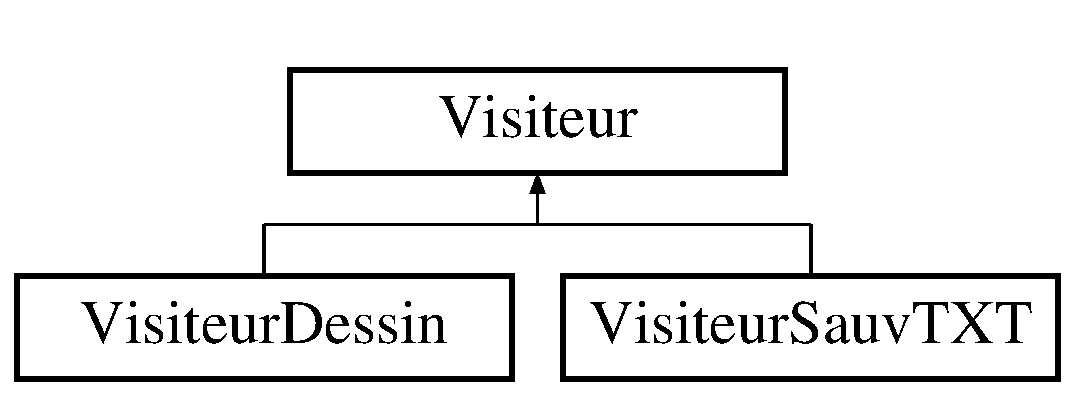
\includegraphics[height=2.000000cm]{class_visiteur}
\end{center}
\end{figure}
\subsection*{Public Member Functions}
\begin{DoxyCompactItemize}
\item 
virtual void \hyperlink{class_visiteur_ab63ea127a0ac3cfa12c4cbdd9d9c8eb2}{visite} (const \hyperlink{class_segment}{Segment} $\ast$s) const =0
\begin{DoxyCompactList}\small\item\em Méthode virtuelle pure, va être appelée par un segment. \end{DoxyCompactList}\item 
virtual void \hyperlink{class_visiteur_a0af8611572f009ff37b9429facc7eaec}{visite} (const \hyperlink{class_cercle}{Cercle} $\ast$c) const =0
\begin{DoxyCompactList}\small\item\em Méthode virtuelle pure, va être appelée par un cercle. \end{DoxyCompactList}\item 
virtual void \hyperlink{class_visiteur_a65332165fada93947fbad9a4d9eebf2c}{visite} (const \hyperlink{class_triangle}{Triangle} $\ast$t) const =0
\begin{DoxyCompactList}\small\item\em Méthode virtuelle pure, va être appelée par un triangle. \end{DoxyCompactList}\item 
virtual void \hyperlink{class_visiteur_a0a7c596d84a8750e3a670330a1001538}{visite} (const \hyperlink{class_polygone}{Polygone} $\ast$s) const =0
\begin{DoxyCompactList}\small\item\em Méthode virtuelle pure, va être appelée par un polygone. \end{DoxyCompactList}\item 
virtual void \hyperlink{class_visiteur_a812aa03fad51d8aec386f8df7f9b5353}{visite} (const \hyperlink{class_groupe}{Groupe} $\ast$g) const =0
\begin{DoxyCompactList}\small\item\em Méthode virtuelle pure, va être appelée par un groupe. \end{DoxyCompactList}\end{DoxyCompactItemize}


\subsection{Member Function Documentation}
\mbox{\Hypertarget{class_visiteur_ab63ea127a0ac3cfa12c4cbdd9d9c8eb2}\label{class_visiteur_ab63ea127a0ac3cfa12c4cbdd9d9c8eb2}} 
\index{Visiteur@{Visiteur}!visite@{visite}}
\index{visite@{visite}!Visiteur@{Visiteur}}
\subsubsection{\texorpdfstring{visite()}{visite()}\hspace{0.1cm}{\footnotesize\ttfamily [1/5]}}
{\footnotesize\ttfamily virtual void Visiteur\+::visite (\begin{DoxyParamCaption}\item[{const \hyperlink{class_segment}{Segment} $\ast$}]{s }\end{DoxyParamCaption}) const\hspace{0.3cm}{\ttfamily [pure virtual]}}



Méthode virtuelle pure, va être appelée par un segment. 



Implemented in \hyperlink{class_visiteur_sauv_t_x_t_a9c5e3b9172f4ee5aa3af9d936a0f8c73}{Visiteur\+Sauv\+T\+XT}, and \hyperlink{class_visiteur_dessin_a39d12a331fcc80c183fc706cdb2d394a}{Visiteur\+Dessin}.

\mbox{\Hypertarget{class_visiteur_a0af8611572f009ff37b9429facc7eaec}\label{class_visiteur_a0af8611572f009ff37b9429facc7eaec}} 
\index{Visiteur@{Visiteur}!visite@{visite}}
\index{visite@{visite}!Visiteur@{Visiteur}}
\subsubsection{\texorpdfstring{visite()}{visite()}\hspace{0.1cm}{\footnotesize\ttfamily [2/5]}}
{\footnotesize\ttfamily virtual void Visiteur\+::visite (\begin{DoxyParamCaption}\item[{const \hyperlink{class_cercle}{Cercle} $\ast$}]{c }\end{DoxyParamCaption}) const\hspace{0.3cm}{\ttfamily [pure virtual]}}



Méthode virtuelle pure, va être appelée par un cercle. 



Implemented in \hyperlink{class_visiteur_sauv_t_x_t_a9e6ae75c4c4cb3f4684895721ac2753f}{Visiteur\+Sauv\+T\+XT}, and \hyperlink{class_visiteur_dessin_ab757769d7c4bf7eac6263eecc8554896}{Visiteur\+Dessin}.

\mbox{\Hypertarget{class_visiteur_a65332165fada93947fbad9a4d9eebf2c}\label{class_visiteur_a65332165fada93947fbad9a4d9eebf2c}} 
\index{Visiteur@{Visiteur}!visite@{visite}}
\index{visite@{visite}!Visiteur@{Visiteur}}
\subsubsection{\texorpdfstring{visite()}{visite()}\hspace{0.1cm}{\footnotesize\ttfamily [3/5]}}
{\footnotesize\ttfamily virtual void Visiteur\+::visite (\begin{DoxyParamCaption}\item[{const \hyperlink{class_triangle}{Triangle} $\ast$}]{t }\end{DoxyParamCaption}) const\hspace{0.3cm}{\ttfamily [pure virtual]}}



Méthode virtuelle pure, va être appelée par un triangle. 



Implemented in \hyperlink{class_visiteur_sauv_t_x_t_a85ef6d5cdd09ae497ad6a2e4ce72a482}{Visiteur\+Sauv\+T\+XT}, and \hyperlink{class_visiteur_dessin_a8278a3991c52c9d00e5ad5a051faacfe}{Visiteur\+Dessin}.

\mbox{\Hypertarget{class_visiteur_a0a7c596d84a8750e3a670330a1001538}\label{class_visiteur_a0a7c596d84a8750e3a670330a1001538}} 
\index{Visiteur@{Visiteur}!visite@{visite}}
\index{visite@{visite}!Visiteur@{Visiteur}}
\subsubsection{\texorpdfstring{visite()}{visite()}\hspace{0.1cm}{\footnotesize\ttfamily [4/5]}}
{\footnotesize\ttfamily virtual void Visiteur\+::visite (\begin{DoxyParamCaption}\item[{const \hyperlink{class_polygone}{Polygone} $\ast$}]{s }\end{DoxyParamCaption}) const\hspace{0.3cm}{\ttfamily [pure virtual]}}



Méthode virtuelle pure, va être appelée par un polygone. 



Implemented in \hyperlink{class_visiteur_sauv_t_x_t_abaf3f953e31644d64110e156bac9c020}{Visiteur\+Sauv\+T\+XT}, and \hyperlink{class_visiteur_dessin_a59ef1f9a400906300fa4e6d3c1ec0ea1}{Visiteur\+Dessin}.

\mbox{\Hypertarget{class_visiteur_a812aa03fad51d8aec386f8df7f9b5353}\label{class_visiteur_a812aa03fad51d8aec386f8df7f9b5353}} 
\index{Visiteur@{Visiteur}!visite@{visite}}
\index{visite@{visite}!Visiteur@{Visiteur}}
\subsubsection{\texorpdfstring{visite()}{visite()}\hspace{0.1cm}{\footnotesize\ttfamily [5/5]}}
{\footnotesize\ttfamily virtual void Visiteur\+::visite (\begin{DoxyParamCaption}\item[{const \hyperlink{class_groupe}{Groupe} $\ast$}]{g }\end{DoxyParamCaption}) const\hspace{0.3cm}{\ttfamily [pure virtual]}}



Méthode virtuelle pure, va être appelée par un groupe. 



Implemented in \hyperlink{class_visiteur_sauv_t_x_t_ae8812148d83e565dc96302df7cc92049}{Visiteur\+Sauv\+T\+XT}, and \hyperlink{class_visiteur_dessin_a295e7bd446e4650257d0cb8c4d8c9ec5}{Visiteur\+Dessin}.



The documentation for this class was generated from the following file\+:\begin{DoxyCompactItemize}
\item 
C\+:/\+Users/\+Quentin Fixe/\+Desktop/\+P\+P\+I\+L-\/master/\+C\+L\+I\+E\+N\+T/\hyperlink{_visiteur_8h}{Visiteur.\+h}\end{DoxyCompactItemize}

\hypertarget{class_visiteur_dessin}{}\section{Référence de la classe Visiteur\+Dessin}
\label{class_visiteur_dessin}\index{VisiteurDessin@{VisiteurDessin}}
Graphe d\textquotesingle{}héritage de Visiteur\+Dessin\+:\begin{figure}[H]
\begin{center}
\leavevmode
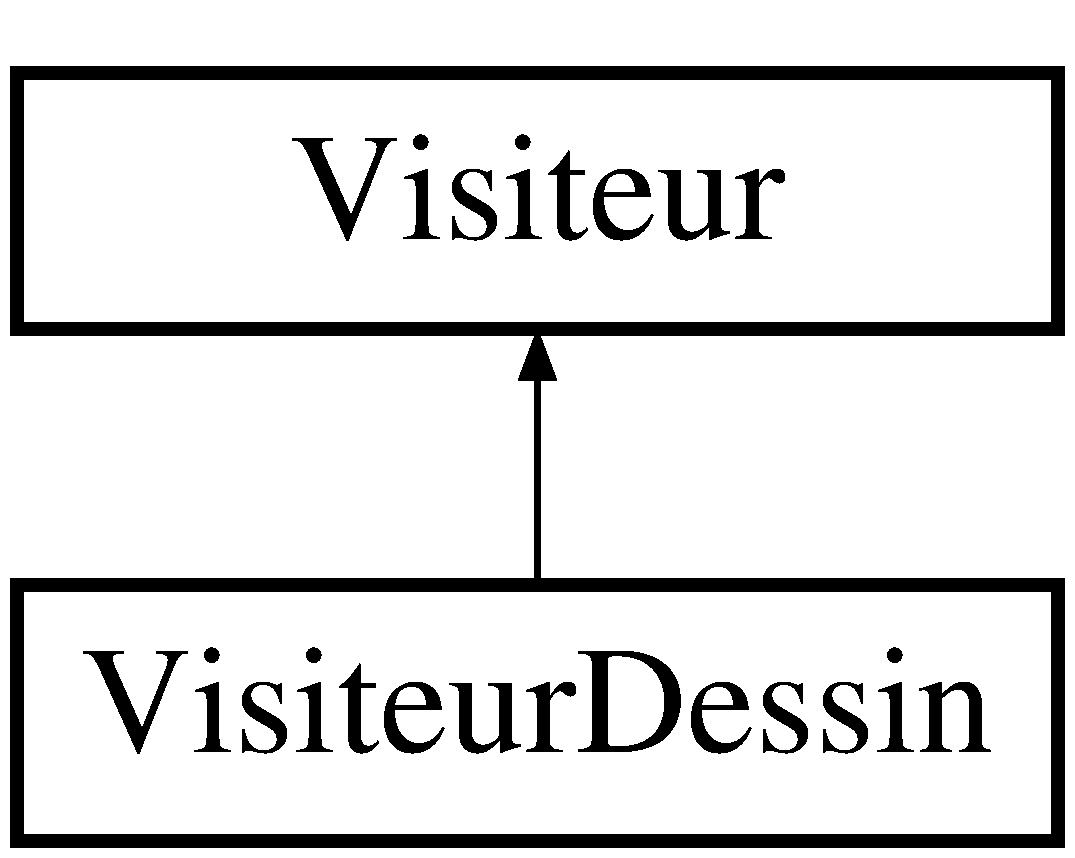
\includegraphics[height=2.000000cm]{class_visiteur_dessin}
\end{center}
\end{figure}
\subsection*{Fonctions membres publiques}
\begin{DoxyCompactItemize}
\item 
virtual void \mbox{\hyperlink{class_visiteur_dessin_a39d12a331fcc80c183fc706cdb2d394a}{visite}} (const \mbox{\hyperlink{class_segment}{Segment}} $\ast$s) const
\begin{DoxyCompactList}\small\item\em Initialise une connexion vers le serveur, dessine un segment puis ferme la connexion. \end{DoxyCompactList}\item 
virtual void \mbox{\hyperlink{class_visiteur_dessin_ab757769d7c4bf7eac6263eecc8554896}{visite}} (const \mbox{\hyperlink{class_cercle}{Cercle}} $\ast$c) const
\begin{DoxyCompactList}\small\item\em Initialise une connexion vers le serveur, dessine un cercle puis ferme la connexion. \end{DoxyCompactList}\item 
virtual void \mbox{\hyperlink{class_visiteur_dessin_a8278a3991c52c9d00e5ad5a051faacfe}{visite}} (const \mbox{\hyperlink{class_triangle}{Triangle}} $\ast$t) const
\begin{DoxyCompactList}\small\item\em Initialise une connexion vers le serveur, dessine un triangle puis ferme la connexion. \end{DoxyCompactList}\item 
virtual void \mbox{\hyperlink{class_visiteur_dessin_a59ef1f9a400906300fa4e6d3c1ec0ea1}{visite}} (const \mbox{\hyperlink{class_polygone}{Polygone}} $\ast$p) const
\begin{DoxyCompactList}\small\item\em Initialise une connexion vers le serveur, dessine un polygone puis ferme la connexion. \end{DoxyCompactList}\item 
virtual void \mbox{\hyperlink{class_visiteur_dessin_a295e7bd446e4650257d0cb8c4d8c9ec5}{visite}} (const \mbox{\hyperlink{class_groupe}{Groupe}} $\ast$g) const
\begin{DoxyCompactList}\small\item\em Initialise une connexion vers le serveur, dessine un groupe puis ferme la connexion. \end{DoxyCompactList}\end{DoxyCompactItemize}


\subsection{Documentation des fonctions membres}
\mbox{\Hypertarget{class_visiteur_dessin_a39d12a331fcc80c183fc706cdb2d394a}\label{class_visiteur_dessin_a39d12a331fcc80c183fc706cdb2d394a}} 
\index{VisiteurDessin@{VisiteurDessin}!visite@{visite}}
\index{visite@{visite}!VisiteurDessin@{VisiteurDessin}}
\subsubsection{\texorpdfstring{visite()}{visite()}\hspace{0.1cm}{\footnotesize\ttfamily [1/5]}}
{\footnotesize\ttfamily void Visiteur\+Dessin\+::visite (\begin{DoxyParamCaption}\item[{const \mbox{\hyperlink{class_segment}{Segment}} $\ast$}]{s }\end{DoxyParamCaption}) const\hspace{0.3cm}{\ttfamily [virtual]}}



Initialise une connexion vers le serveur, dessine un segment puis ferme la connexion. 


\begin{DoxyParams}{Paramètres}
{\em s} & Pointeur sur le segment à dessiner \\
\hline
\end{DoxyParams}


Implémente \mbox{\hyperlink{class_visiteur_ab63ea127a0ac3cfa12c4cbdd9d9c8eb2}{Visiteur}}.

\mbox{\Hypertarget{class_visiteur_dessin_ab757769d7c4bf7eac6263eecc8554896}\label{class_visiteur_dessin_ab757769d7c4bf7eac6263eecc8554896}} 
\index{VisiteurDessin@{VisiteurDessin}!visite@{visite}}
\index{visite@{visite}!VisiteurDessin@{VisiteurDessin}}
\subsubsection{\texorpdfstring{visite()}{visite()}\hspace{0.1cm}{\footnotesize\ttfamily [2/5]}}
{\footnotesize\ttfamily void Visiteur\+Dessin\+::visite (\begin{DoxyParamCaption}\item[{const \mbox{\hyperlink{class_cercle}{Cercle}} $\ast$}]{c }\end{DoxyParamCaption}) const\hspace{0.3cm}{\ttfamily [virtual]}}



Initialise une connexion vers le serveur, dessine un cercle puis ferme la connexion. 


\begin{DoxyParams}{Paramètres}
{\em s} & Pointeur sur le cercle à dessiner \\
\hline
\end{DoxyParams}


Implémente \mbox{\hyperlink{class_visiteur_a0af8611572f009ff37b9429facc7eaec}{Visiteur}}.

\mbox{\Hypertarget{class_visiteur_dessin_a8278a3991c52c9d00e5ad5a051faacfe}\label{class_visiteur_dessin_a8278a3991c52c9d00e5ad5a051faacfe}} 
\index{VisiteurDessin@{VisiteurDessin}!visite@{visite}}
\index{visite@{visite}!VisiteurDessin@{VisiteurDessin}}
\subsubsection{\texorpdfstring{visite()}{visite()}\hspace{0.1cm}{\footnotesize\ttfamily [3/5]}}
{\footnotesize\ttfamily void Visiteur\+Dessin\+::visite (\begin{DoxyParamCaption}\item[{const \mbox{\hyperlink{class_triangle}{Triangle}} $\ast$}]{t }\end{DoxyParamCaption}) const\hspace{0.3cm}{\ttfamily [virtual]}}



Initialise une connexion vers le serveur, dessine un triangle puis ferme la connexion. 


\begin{DoxyParams}{Paramètres}
{\em s} & Pointeur sur le triangle à dessiner \\
\hline
\end{DoxyParams}


Implémente \mbox{\hyperlink{class_visiteur_a65332165fada93947fbad9a4d9eebf2c}{Visiteur}}.

\mbox{\Hypertarget{class_visiteur_dessin_a59ef1f9a400906300fa4e6d3c1ec0ea1}\label{class_visiteur_dessin_a59ef1f9a400906300fa4e6d3c1ec0ea1}} 
\index{VisiteurDessin@{VisiteurDessin}!visite@{visite}}
\index{visite@{visite}!VisiteurDessin@{VisiteurDessin}}
\subsubsection{\texorpdfstring{visite()}{visite()}\hspace{0.1cm}{\footnotesize\ttfamily [4/5]}}
{\footnotesize\ttfamily void Visiteur\+Dessin\+::visite (\begin{DoxyParamCaption}\item[{const \mbox{\hyperlink{class_polygone}{Polygone}} $\ast$}]{p }\end{DoxyParamCaption}) const\hspace{0.3cm}{\ttfamily [virtual]}}



Initialise une connexion vers le serveur, dessine un polygone puis ferme la connexion. 


\begin{DoxyParams}{Paramètres}
{\em s} & Pointeur sur le polygone à dessiner \\
\hline
\end{DoxyParams}


Implémente \mbox{\hyperlink{class_visiteur_a0a7c596d84a8750e3a670330a1001538}{Visiteur}}.

\mbox{\Hypertarget{class_visiteur_dessin_a295e7bd446e4650257d0cb8c4d8c9ec5}\label{class_visiteur_dessin_a295e7bd446e4650257d0cb8c4d8c9ec5}} 
\index{VisiteurDessin@{VisiteurDessin}!visite@{visite}}
\index{visite@{visite}!VisiteurDessin@{VisiteurDessin}}
\subsubsection{\texorpdfstring{visite()}{visite()}\hspace{0.1cm}{\footnotesize\ttfamily [5/5]}}
{\footnotesize\ttfamily void Visiteur\+Dessin\+::visite (\begin{DoxyParamCaption}\item[{const \mbox{\hyperlink{class_groupe}{Groupe}} $\ast$}]{g }\end{DoxyParamCaption}) const\hspace{0.3cm}{\ttfamily [virtual]}}



Initialise une connexion vers le serveur, dessine un groupe puis ferme la connexion. 


\begin{DoxyParams}{Paramètres}
{\em s} & Pointeur sur le groupe à dessiner \\
\hline
\end{DoxyParams}


Implémente \mbox{\hyperlink{class_visiteur_a812aa03fad51d8aec386f8df7f9b5353}{Visiteur}}.



La documentation de cette classe a été générée à partir des fichiers suivants \+:\begin{DoxyCompactItemize}
\item 
\mbox{\hyperlink{_visiteur_dessin_8h}{Visiteur\+Dessin.\+h}}\item 
Visiteur\+Dessin.\+cpp\end{DoxyCompactItemize}

\hypertarget{class_visiteur_sauv_t_x_t}{}\section{Visiteur\+Sauv\+T\+XT Class Reference}
\label{class_visiteur_sauv_t_x_t}\index{Visiteur\+Sauv\+T\+XT@{Visiteur\+Sauv\+T\+XT}}


{\ttfamily \#include $<$Visiteur\+Sauv\+T\+X\+T.\+h$>$}

Inheritance diagram for Visiteur\+Sauv\+T\+XT\+:\begin{figure}[H]
\begin{center}
\leavevmode
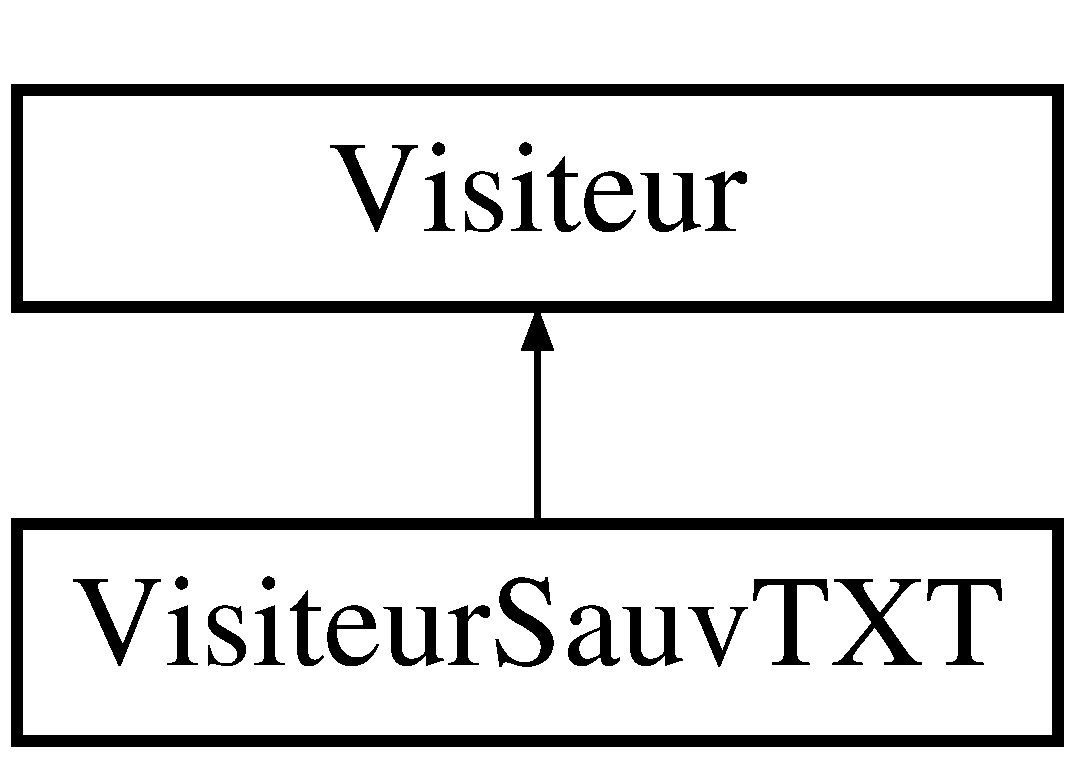
\includegraphics[height=2.000000cm]{class_visiteur_sauv_t_x_t}
\end{center}
\end{figure}
\subsection*{Public Member Functions}
\begin{DoxyCompactItemize}
\item 
virtual void \hyperlink{class_visiteur_sauv_t_x_t_a9c5e3b9172f4ee5aa3af9d936a0f8c73}{visite} (const \hyperlink{class_segment}{Segment} $\ast$s) const
\begin{DoxyCompactList}\small\item\em Sauvegarde un segment dans un fichier. \end{DoxyCompactList}\item 
virtual void \hyperlink{class_visiteur_sauv_t_x_t_a9e6ae75c4c4cb3f4684895721ac2753f}{visite} (const \hyperlink{class_cercle}{Cercle} $\ast$c) const
\begin{DoxyCompactList}\small\item\em Sauvegarde un cercle dans un fichier. \end{DoxyCompactList}\item 
virtual void \hyperlink{class_visiteur_sauv_t_x_t_a85ef6d5cdd09ae497ad6a2e4ce72a482}{visite} (const \hyperlink{class_triangle}{Triangle} $\ast$t) const
\begin{DoxyCompactList}\small\item\em Sauvegarde un triangle dans un fichier. \end{DoxyCompactList}\item 
virtual void \hyperlink{class_visiteur_sauv_t_x_t_abaf3f953e31644d64110e156bac9c020}{visite} (const \hyperlink{class_polygone}{Polygone} $\ast$p) const
\begin{DoxyCompactList}\small\item\em Sauvegarde un polygone dans un fichier. \end{DoxyCompactList}\item 
virtual void \hyperlink{class_visiteur_sauv_t_x_t_ae8812148d83e565dc96302df7cc92049}{visite} (const \hyperlink{class_groupe}{Groupe} $\ast$g) const
\begin{DoxyCompactList}\small\item\em Sauvegarde un groupe dans un fichier. \end{DoxyCompactList}\end{DoxyCompactItemize}


\subsection{Member Function Documentation}
\mbox{\Hypertarget{class_visiteur_sauv_t_x_t_a9c5e3b9172f4ee5aa3af9d936a0f8c73}\label{class_visiteur_sauv_t_x_t_a9c5e3b9172f4ee5aa3af9d936a0f8c73}} 
\index{Visiteur\+Sauv\+T\+XT@{Visiteur\+Sauv\+T\+XT}!visite@{visite}}
\index{visite@{visite}!Visiteur\+Sauv\+T\+XT@{Visiteur\+Sauv\+T\+XT}}
\subsubsection{\texorpdfstring{visite()}{visite()}\hspace{0.1cm}{\footnotesize\ttfamily [1/5]}}
{\footnotesize\ttfamily void Visiteur\+Sauv\+T\+X\+T\+::visite (\begin{DoxyParamCaption}\item[{const \hyperlink{class_segment}{Segment} $\ast$}]{s }\end{DoxyParamCaption}) const\hspace{0.3cm}{\ttfamily [virtual]}}



Sauvegarde un segment dans un fichier. 


\begin{DoxyParams}{Parameters}
{\em s} & Pointeur sur le segment � sauvegarder \\
\hline
\end{DoxyParams}


Implements \hyperlink{class_visiteur_ab63ea127a0ac3cfa12c4cbdd9d9c8eb2}{Visiteur}.

\mbox{\Hypertarget{class_visiteur_sauv_t_x_t_a9e6ae75c4c4cb3f4684895721ac2753f}\label{class_visiteur_sauv_t_x_t_a9e6ae75c4c4cb3f4684895721ac2753f}} 
\index{Visiteur\+Sauv\+T\+XT@{Visiteur\+Sauv\+T\+XT}!visite@{visite}}
\index{visite@{visite}!Visiteur\+Sauv\+T\+XT@{Visiteur\+Sauv\+T\+XT}}
\subsubsection{\texorpdfstring{visite()}{visite()}\hspace{0.1cm}{\footnotesize\ttfamily [2/5]}}
{\footnotesize\ttfamily void Visiteur\+Sauv\+T\+X\+T\+::visite (\begin{DoxyParamCaption}\item[{const \hyperlink{class_cercle}{Cercle} $\ast$}]{c }\end{DoxyParamCaption}) const\hspace{0.3cm}{\ttfamily [virtual]}}



Sauvegarde un cercle dans un fichier. 


\begin{DoxyParams}{Parameters}
{\em s} & Pointeur sur le cercle � sauvegarder \\
\hline
\end{DoxyParams}


Implements \hyperlink{class_visiteur_a0af8611572f009ff37b9429facc7eaec}{Visiteur}.

\mbox{\Hypertarget{class_visiteur_sauv_t_x_t_a85ef6d5cdd09ae497ad6a2e4ce72a482}\label{class_visiteur_sauv_t_x_t_a85ef6d5cdd09ae497ad6a2e4ce72a482}} 
\index{Visiteur\+Sauv\+T\+XT@{Visiteur\+Sauv\+T\+XT}!visite@{visite}}
\index{visite@{visite}!Visiteur\+Sauv\+T\+XT@{Visiteur\+Sauv\+T\+XT}}
\subsubsection{\texorpdfstring{visite()}{visite()}\hspace{0.1cm}{\footnotesize\ttfamily [3/5]}}
{\footnotesize\ttfamily void Visiteur\+Sauv\+T\+X\+T\+::visite (\begin{DoxyParamCaption}\item[{const \hyperlink{class_triangle}{Triangle} $\ast$}]{t }\end{DoxyParamCaption}) const\hspace{0.3cm}{\ttfamily [virtual]}}



Sauvegarde un triangle dans un fichier. 


\begin{DoxyParams}{Parameters}
{\em s} & Pointeur sur le triangle � sauvegarder \\
\hline
\end{DoxyParams}


Implements \hyperlink{class_visiteur_a65332165fada93947fbad9a4d9eebf2c}{Visiteur}.

\mbox{\Hypertarget{class_visiteur_sauv_t_x_t_abaf3f953e31644d64110e156bac9c020}\label{class_visiteur_sauv_t_x_t_abaf3f953e31644d64110e156bac9c020}} 
\index{Visiteur\+Sauv\+T\+XT@{Visiteur\+Sauv\+T\+XT}!visite@{visite}}
\index{visite@{visite}!Visiteur\+Sauv\+T\+XT@{Visiteur\+Sauv\+T\+XT}}
\subsubsection{\texorpdfstring{visite()}{visite()}\hspace{0.1cm}{\footnotesize\ttfamily [4/5]}}
{\footnotesize\ttfamily void Visiteur\+Sauv\+T\+X\+T\+::visite (\begin{DoxyParamCaption}\item[{const \hyperlink{class_polygone}{Polygone} $\ast$}]{p }\end{DoxyParamCaption}) const\hspace{0.3cm}{\ttfamily [virtual]}}



Sauvegarde un polygone dans un fichier. 


\begin{DoxyParams}{Parameters}
{\em s} & Pointeur sur le polygone � sauvegarder \\
\hline
\end{DoxyParams}


Implements \hyperlink{class_visiteur_a0a7c596d84a8750e3a670330a1001538}{Visiteur}.

\mbox{\Hypertarget{class_visiteur_sauv_t_x_t_ae8812148d83e565dc96302df7cc92049}\label{class_visiteur_sauv_t_x_t_ae8812148d83e565dc96302df7cc92049}} 
\index{Visiteur\+Sauv\+T\+XT@{Visiteur\+Sauv\+T\+XT}!visite@{visite}}
\index{visite@{visite}!Visiteur\+Sauv\+T\+XT@{Visiteur\+Sauv\+T\+XT}}
\subsubsection{\texorpdfstring{visite()}{visite()}\hspace{0.1cm}{\footnotesize\ttfamily [5/5]}}
{\footnotesize\ttfamily void Visiteur\+Sauv\+T\+X\+T\+::visite (\begin{DoxyParamCaption}\item[{const \hyperlink{class_groupe}{Groupe} $\ast$}]{g }\end{DoxyParamCaption}) const\hspace{0.3cm}{\ttfamily [virtual]}}



Sauvegarde un groupe dans un fichier. 


\begin{DoxyParams}{Parameters}
{\em s} & Pointeur sur le groupe � sauvegarder \\
\hline
\end{DoxyParams}


Implements \hyperlink{class_visiteur_a812aa03fad51d8aec386f8df7f9b5353}{Visiteur}.



The documentation for this class was generated from the following files\+:\begin{DoxyCompactItemize}
\item 
C\+:/\+Users/\+Quentin Fixe/\+Desktop/\+P\+P\+I\+L-\/master/\+C\+L\+I\+E\+N\+T/\hyperlink{_visiteur_sauv_t_x_t_8h}{Visiteur\+Sauv\+T\+X\+T.\+h}\item 
C\+:/\+Users/\+Quentin Fixe/\+Desktop/\+P\+P\+I\+L-\/master/\+C\+L\+I\+E\+N\+T/\hyperlink{_visiteur_sauv_t_x_t_8cpp}{Visiteur\+Sauv\+T\+X\+T.\+cpp}\end{DoxyCompactItemize}

\chapter{File Documentation}
\hypertarget{_cercle_8cpp}{}\section{C\+:/\+Users/\+Quentin Fixe/\+Desktop/\+P\+P\+I\+L-\/master/\+C\+L\+I\+E\+N\+T/\+Cercle.cpp File Reference}
\label{_cercle_8cpp}\index{C\+:/\+Users/\+Quentin Fixe/\+Desktop/\+P\+P\+I\+L-\/master/\+C\+L\+I\+E\+N\+T/\+Cercle.\+cpp@{C\+:/\+Users/\+Quentin Fixe/\+Desktop/\+P\+P\+I\+L-\/master/\+C\+L\+I\+E\+N\+T/\+Cercle.\+cpp}}
{\ttfamily \#include \char`\"{}Cercle.\+h\char`\"{}}\newline
{\ttfamily \#include \char`\"{}Visiteur\+Sauv\+T\+X\+T.\+h\char`\"{}}\newline
{\ttfamily \#include \char`\"{}Visiteur\+Dessin.\+h\char`\"{}}\newline

\hypertarget{_cercle_8h}{}\section{Référence du fichier Cercle.\+h}
\label{_cercle_8h}\index{Cercle.h@{Cercle.h}}


Classe cercle qui repr�sente une forme sp�ciale (cercle)  


{\ttfamily \#include \char`\"{}Forme.\+h\char`\"{}}\newline
\subsection*{Classes}
\begin{DoxyCompactItemize}
\item 
class \mbox{\hyperlink{class_cercle}{Cercle}}
\end{DoxyCompactItemize}


\subsection{Description détaillée}
Classe cercle qui repr�sente une forme sp�ciale (cercle) 


\hypertarget{_charger_forme_8h}{}\section{C\+:/\+Users/\+Quentin Fixe/\+Desktop/\+P\+P\+I\+L-\/master/\+C\+L\+I\+E\+N\+T/\+Charger\+Forme.h File Reference}
\label{_charger_forme_8h}\index{C\+:/\+Users/\+Quentin Fixe/\+Desktop/\+P\+P\+I\+L-\/master/\+C\+L\+I\+E\+N\+T/\+Charger\+Forme.\+h@{C\+:/\+Users/\+Quentin Fixe/\+Desktop/\+P\+P\+I\+L-\/master/\+C\+L\+I\+E\+N\+T/\+Charger\+Forme.\+h}}
{\ttfamily \#include \char`\"{}Forme.\+h\char`\"{}}\newline
\subsection*{Classes}
\begin{DoxyCompactItemize}
\item 
class \hyperlink{class_charger_forme}{Charger\+Forme}
\end{DoxyCompactItemize}

\hypertarget{_charger_forme_c_o_r_8cpp}{}\section{C\+:/\+Users/\+Quentin Fixe/\+Desktop/\+P\+P\+I\+L-\/master/\+C\+L\+I\+E\+N\+T/\+Charger\+Forme\+C\+OR.cpp File Reference}
\label{_charger_forme_c_o_r_8cpp}\index{C\+:/\+Users/\+Quentin Fixe/\+Desktop/\+P\+P\+I\+L-\/master/\+C\+L\+I\+E\+N\+T/\+Charger\+Forme\+C\+O\+R.\+cpp@{C\+:/\+Users/\+Quentin Fixe/\+Desktop/\+P\+P\+I\+L-\/master/\+C\+L\+I\+E\+N\+T/\+Charger\+Forme\+C\+O\+R.\+cpp}}
{\ttfamily \#include \char`\"{}Charger\+Forme\+C\+O\+R.\+h\char`\"{}}\newline
{\ttfamily \#include \char`\"{}Constantes.\+h\char`\"{}}\newline
{\ttfamily \#include $<$fstream$>$}\newline

\hypertarget{_charger_forme_c_o_r_8h}{}\section{C\+:/\+Users/\+Quentin Fixe/\+Desktop/\+P\+P\+I\+L-\/master/\+C\+L\+I\+E\+N\+T/\+Charger\+Forme\+C\+OR.h File Reference}
\label{_charger_forme_c_o_r_8h}\index{C\+:/\+Users/\+Quentin Fixe/\+Desktop/\+P\+P\+I\+L-\/master/\+C\+L\+I\+E\+N\+T/\+Charger\+Forme\+C\+O\+R.\+h@{C\+:/\+Users/\+Quentin Fixe/\+Desktop/\+P\+P\+I\+L-\/master/\+C\+L\+I\+E\+N\+T/\+Charger\+Forme\+C\+O\+R.\+h}}
{\ttfamily \#include \char`\"{}Charger\+Forme.\+h\char`\"{}}\newline
\subsection*{Classes}
\begin{DoxyCompactItemize}
\item 
class \hyperlink{class_charger_forme_c_o_r}{Charger\+Forme\+C\+OR}
\end{DoxyCompactItemize}

\hypertarget{_charger_forme_c_o_r_cercle_8cpp}{}\section{C\+:/\+Users/\+Quentin Fixe/\+Desktop/\+P\+P\+I\+L-\/master/\+C\+L\+I\+E\+N\+T/\+Charger\+Forme\+C\+O\+R\+Cercle.cpp File Reference}
\label{_charger_forme_c_o_r_cercle_8cpp}\index{C\+:/\+Users/\+Quentin Fixe/\+Desktop/\+P\+P\+I\+L-\/master/\+C\+L\+I\+E\+N\+T/\+Charger\+Forme\+C\+O\+R\+Cercle.\+cpp@{C\+:/\+Users/\+Quentin Fixe/\+Desktop/\+P\+P\+I\+L-\/master/\+C\+L\+I\+E\+N\+T/\+Charger\+Forme\+C\+O\+R\+Cercle.\+cpp}}
{\ttfamily \#include \char`\"{}Charger\+Forme\+C\+O\+R\+Cercle.\+h\char`\"{}}\newline
{\ttfamily \#include \char`\"{}Cercle.\+h\char`\"{}}\newline

\hypertarget{_charger_forme_c_o_r_cercle_8h}{}\section{C\+:/\+Users/\+Quentin Fixe/\+Desktop/\+P\+P\+I\+L-\/master/\+C\+L\+I\+E\+N\+T/\+Charger\+Forme\+C\+O\+R\+Cercle.h File Reference}
\label{_charger_forme_c_o_r_cercle_8h}\index{C\+:/\+Users/\+Quentin Fixe/\+Desktop/\+P\+P\+I\+L-\/master/\+C\+L\+I\+E\+N\+T/\+Charger\+Forme\+C\+O\+R\+Cercle.\+h@{C\+:/\+Users/\+Quentin Fixe/\+Desktop/\+P\+P\+I\+L-\/master/\+C\+L\+I\+E\+N\+T/\+Charger\+Forme\+C\+O\+R\+Cercle.\+h}}
{\ttfamily \#include \char`\"{}Charger\+Forme\+C\+O\+R.\+h\char`\"{}}\newline
\subsection*{Classes}
\begin{DoxyCompactItemize}
\item 
class \hyperlink{class_charger_forme_c_o_r_cercle}{Charger\+Forme\+C\+O\+R\+Cercle}
\end{DoxyCompactItemize}

\hypertarget{_charger_forme_c_o_r_groupe_8cpp}{}\section{C\+:/\+Users/\+Quentin Fixe/\+Desktop/\+P\+P\+I\+L-\/master/\+C\+L\+I\+E\+N\+T/\+Charger\+Forme\+C\+O\+R\+Groupe.cpp File Reference}
\label{_charger_forme_c_o_r_groupe_8cpp}\index{C\+:/\+Users/\+Quentin Fixe/\+Desktop/\+P\+P\+I\+L-\/master/\+C\+L\+I\+E\+N\+T/\+Charger\+Forme\+C\+O\+R\+Groupe.\+cpp@{C\+:/\+Users/\+Quentin Fixe/\+Desktop/\+P\+P\+I\+L-\/master/\+C\+L\+I\+E\+N\+T/\+Charger\+Forme\+C\+O\+R\+Groupe.\+cpp}}
{\ttfamily \#include \char`\"{}Charger\+Forme\+C\+O\+R\+Groupe.\+h\char`\"{}}\newline
{\ttfamily \#include \char`\"{}Groupe.\+h\char`\"{}}\newline
{\ttfamily \#include \char`\"{}C\+O\+R.\+h\char`\"{}}\newline

\hypertarget{_charger_forme_c_o_r_groupe_8h}{}\section{C\+:/\+Users/\+Quentin Fixe/\+Desktop/\+P\+P\+I\+L-\/master/\+C\+L\+I\+E\+N\+T/\+Charger\+Forme\+C\+O\+R\+Groupe.h File Reference}
\label{_charger_forme_c_o_r_groupe_8h}\index{C\+:/\+Users/\+Quentin Fixe/\+Desktop/\+P\+P\+I\+L-\/master/\+C\+L\+I\+E\+N\+T/\+Charger\+Forme\+C\+O\+R\+Groupe.\+h@{C\+:/\+Users/\+Quentin Fixe/\+Desktop/\+P\+P\+I\+L-\/master/\+C\+L\+I\+E\+N\+T/\+Charger\+Forme\+C\+O\+R\+Groupe.\+h}}
{\ttfamily \#include \char`\"{}Charger\+Forme\+C\+O\+R.\+h\char`\"{}}\newline
\subsection*{Classes}
\begin{DoxyCompactItemize}
\item 
class \hyperlink{class_charger_forme_c_o_r_groupe}{Charger\+Forme\+C\+O\+R\+Groupe}
\end{DoxyCompactItemize}

\hypertarget{_charger_forme_c_o_r_polygone_8cpp}{}\section{C\+:/\+Users/\+Quentin Fixe/\+Desktop/\+P\+P\+I\+L-\/master/\+C\+L\+I\+E\+N\+T/\+Charger\+Forme\+C\+O\+R\+Polygone.cpp File Reference}
\label{_charger_forme_c_o_r_polygone_8cpp}\index{C\+:/\+Users/\+Quentin Fixe/\+Desktop/\+P\+P\+I\+L-\/master/\+C\+L\+I\+E\+N\+T/\+Charger\+Forme\+C\+O\+R\+Polygone.\+cpp@{C\+:/\+Users/\+Quentin Fixe/\+Desktop/\+P\+P\+I\+L-\/master/\+C\+L\+I\+E\+N\+T/\+Charger\+Forme\+C\+O\+R\+Polygone.\+cpp}}
{\ttfamily \#include \char`\"{}Charger\+Forme\+C\+O\+R\+Polygone.\+h\char`\"{}}\newline
{\ttfamily \#include \char`\"{}Polygone.\+h\char`\"{}}\newline

\hypertarget{_charger_forme_c_o_r_polygone_8h}{}\section{C\+:/\+Users/\+Quentin Fixe/\+Desktop/\+P\+P\+I\+L-\/master/\+C\+L\+I\+E\+N\+T/\+Charger\+Forme\+C\+O\+R\+Polygone.h File Reference}
\label{_charger_forme_c_o_r_polygone_8h}\index{C\+:/\+Users/\+Quentin Fixe/\+Desktop/\+P\+P\+I\+L-\/master/\+C\+L\+I\+E\+N\+T/\+Charger\+Forme\+C\+O\+R\+Polygone.\+h@{C\+:/\+Users/\+Quentin Fixe/\+Desktop/\+P\+P\+I\+L-\/master/\+C\+L\+I\+E\+N\+T/\+Charger\+Forme\+C\+O\+R\+Polygone.\+h}}
{\ttfamily \#include \char`\"{}Charger\+Forme\+C\+O\+R.\+h\char`\"{}}\newline
\subsection*{Classes}
\begin{DoxyCompactItemize}
\item 
class \hyperlink{class_charger_forme_c_o_r_polygone}{Charger\+Forme\+C\+O\+R\+Polygone}
\end{DoxyCompactItemize}

\hypertarget{_charger_forme_c_o_r_segment_8cpp}{}\section{C\+:/\+Users/\+Quentin Fixe/\+Desktop/\+P\+P\+I\+L-\/master/\+C\+L\+I\+E\+N\+T/\+Charger\+Forme\+C\+O\+R\+Segment.cpp File Reference}
\label{_charger_forme_c_o_r_segment_8cpp}\index{C\+:/\+Users/\+Quentin Fixe/\+Desktop/\+P\+P\+I\+L-\/master/\+C\+L\+I\+E\+N\+T/\+Charger\+Forme\+C\+O\+R\+Segment.\+cpp@{C\+:/\+Users/\+Quentin Fixe/\+Desktop/\+P\+P\+I\+L-\/master/\+C\+L\+I\+E\+N\+T/\+Charger\+Forme\+C\+O\+R\+Segment.\+cpp}}
{\ttfamily \#include \char`\"{}Charger\+Forme\+C\+O\+R\+Segment.\+h\char`\"{}}\newline
{\ttfamily \#include \char`\"{}Segment.\+h\char`\"{}}\newline

\hypertarget{_charger_forme_c_o_r_segment_8h}{}\section{C\+:/\+Users/\+Quentin Fixe/\+Desktop/\+P\+P\+I\+L-\/master/\+C\+L\+I\+E\+N\+T/\+Charger\+Forme\+C\+O\+R\+Segment.h File Reference}
\label{_charger_forme_c_o_r_segment_8h}\index{C\+:/\+Users/\+Quentin Fixe/\+Desktop/\+P\+P\+I\+L-\/master/\+C\+L\+I\+E\+N\+T/\+Charger\+Forme\+C\+O\+R\+Segment.\+h@{C\+:/\+Users/\+Quentin Fixe/\+Desktop/\+P\+P\+I\+L-\/master/\+C\+L\+I\+E\+N\+T/\+Charger\+Forme\+C\+O\+R\+Segment.\+h}}
{\ttfamily \#include \char`\"{}Charger\+Forme\+C\+O\+R.\+h\char`\"{}}\newline
\subsection*{Classes}
\begin{DoxyCompactItemize}
\item 
class \hyperlink{class_charger_forme_c_o_r_segment}{Charger\+Forme\+C\+O\+R\+Segment}
\end{DoxyCompactItemize}

\hypertarget{_charger_forme_c_o_r_triangle_8cpp}{}\section{C\+:/\+Users/\+Quentin Fixe/\+Desktop/\+P\+P\+I\+L-\/master/\+C\+L\+I\+E\+N\+T/\+Charger\+Forme\+C\+O\+R\+Triangle.cpp File Reference}
\label{_charger_forme_c_o_r_triangle_8cpp}\index{C\+:/\+Users/\+Quentin Fixe/\+Desktop/\+P\+P\+I\+L-\/master/\+C\+L\+I\+E\+N\+T/\+Charger\+Forme\+C\+O\+R\+Triangle.\+cpp@{C\+:/\+Users/\+Quentin Fixe/\+Desktop/\+P\+P\+I\+L-\/master/\+C\+L\+I\+E\+N\+T/\+Charger\+Forme\+C\+O\+R\+Triangle.\+cpp}}
{\ttfamily \#include \char`\"{}Charger\+Forme\+C\+O\+R\+Triangle.\+h\char`\"{}}\newline
{\ttfamily \#include \char`\"{}Triangle.\+h\char`\"{}}\newline

\hypertarget{_charger_forme_c_o_r_triangle_8h}{}\section{C\+:/\+Users/\+Quentin Fixe/\+Desktop/\+P\+P\+I\+L-\/master/\+C\+L\+I\+E\+N\+T/\+Charger\+Forme\+C\+O\+R\+Triangle.h File Reference}
\label{_charger_forme_c_o_r_triangle_8h}\index{C\+:/\+Users/\+Quentin Fixe/\+Desktop/\+P\+P\+I\+L-\/master/\+C\+L\+I\+E\+N\+T/\+Charger\+Forme\+C\+O\+R\+Triangle.\+h@{C\+:/\+Users/\+Quentin Fixe/\+Desktop/\+P\+P\+I\+L-\/master/\+C\+L\+I\+E\+N\+T/\+Charger\+Forme\+C\+O\+R\+Triangle.\+h}}
{\ttfamily \#include \char`\"{}Charger\+Forme\+C\+O\+R.\+h\char`\"{}}\newline
\subsection*{Classes}
\begin{DoxyCompactItemize}
\item 
class \hyperlink{class_charger_forme_c_o_r_triangle}{Charger\+Forme\+C\+O\+R\+Triangle}
\end{DoxyCompactItemize}

\hypertarget{_constantes_8h}{}\section{Référence du fichier Constantes.\+h}
\label{_constantes_8h}\index{Constantes.h@{Constantes.h}}


Fichier qui contient toutes les cpnstantes nécessaires au programme.  


{\ttfamily \#include $<$iostream$>$}\newline
{\ttfamily \#include $<$string$>$}\newline
\subsection*{Variables}
\begin{DoxyCompactItemize}
\item 
\mbox{\Hypertarget{_constantes_8h_ae19c9efc0da872e4ddd342debacb600a}\label{_constantes_8h_ae19c9efc0da872e4ddd342debacb600a}} 
const int {\bfseries L\+A\+R\+G\+E\+UR} = 1000
\item 
\mbox{\Hypertarget{_constantes_8h_a869238ab38746d1ed255935b65114f77}\label{_constantes_8h_a869238ab38746d1ed255935b65114f77}} 
const int {\bfseries H\+A\+U\+T\+E\+UR} = 700
\item 
const std\+::string \mbox{\hyperlink{_constantes_8h_a28e43e9ab4691115027597a38fdd85e6}{D\+E\+F\+A\+U\+LT}} = \char`\"{}unknown\char`\"{}
\item 
\mbox{\Hypertarget{_constantes_8h_aacd5164ed9c9701c9073d167eabfe638}\label{_constantes_8h_aacd5164ed9c9701c9073d167eabfe638}} 
const std\+::string {\bfseries B\+L\+A\+CK} = \char`\"{}black\char`\"{}
\item 
\mbox{\Hypertarget{_constantes_8h_abe00a28b292cf705c5a54afc31c5d034}\label{_constantes_8h_abe00a28b292cf705c5a54afc31c5d034}} 
const std\+::string {\bfseries B\+L\+UE} = \char`\"{}blue\char`\"{}
\item 
\mbox{\Hypertarget{_constantes_8h_a1e3de85aa0ad921f6984f3aef7361f99}\label{_constantes_8h_a1e3de85aa0ad921f6984f3aef7361f99}} 
const std\+::string {\bfseries R\+ED} = \char`\"{}red\char`\"{}
\item 
\mbox{\Hypertarget{_constantes_8h_ace790543ffe3663a896a5f074bd2a3ef}\label{_constantes_8h_ace790543ffe3663a896a5f074bd2a3ef}} 
const std\+::string {\bfseries G\+R\+E\+EN} = \char`\"{}green\char`\"{}
\item 
\mbox{\Hypertarget{_constantes_8h_a8bc779337e61d3ab6ad13f81e102f327}\label{_constantes_8h_a8bc779337e61d3ab6ad13f81e102f327}} 
const std\+::string {\bfseries Y\+E\+L\+L\+OW} = \char`\"{}yellow\char`\"{}
\item 
\mbox{\Hypertarget{_constantes_8h_ac1965adc92c3076b04d6cd16f36e8f77}\label{_constantes_8h_ac1965adc92c3076b04d6cd16f36e8f77}} 
const std\+::string {\bfseries C\+Y\+AN} = \char`\"{}cyan\char`\"{}
\item 
\mbox{\Hypertarget{_constantes_8h_a7d9d404a966d10b4a46c76592d881f52}\label{_constantes_8h_a7d9d404a966d10b4a46c76592d881f52}} 
const std\+::string {\bfseries C\+H\+E\+M\+IN} = \char`\"{}.//Sauvgardes.\+txt\char`\"{}
\item 
\mbox{\Hypertarget{_constantes_8h_a952eac791b596a61bba0a133a3bb439f}\label{_constantes_8h_a952eac791b596a61bba0a133a3bb439f}} 
const double {\bfseries PI} = 3.\+14159265358979323846
\end{DoxyCompactItemize}


\subsection{Description détaillée}
Fichier qui contient toutes les cpnstantes nécessaires au programme. 



\subsection{Documentation des variables}
\mbox{\Hypertarget{_constantes_8h_a28e43e9ab4691115027597a38fdd85e6}\label{_constantes_8h_a28e43e9ab4691115027597a38fdd85e6}} 
\index{Constantes.h@{Constantes.h}!DEFAULT@{DEFAULT}}
\index{DEFAULT@{DEFAULT}!Constantes.h@{Constantes.h}}
\subsubsection{\texorpdfstring{DEFAULT}{DEFAULT}}
{\footnotesize\ttfamily const std\+::string D\+E\+F\+A\+U\+LT = \char`\"{}unknown\char`\"{}}

couleurs 
\hypertarget{_c_o_r_8cpp}{}\section{C\+:/\+Users/\+Quentin Fixe/\+Desktop/\+P\+P\+I\+L-\/master/\+C\+L\+I\+E\+N\+T/\+C\+OR.cpp File Reference}
\label{_c_o_r_8cpp}\index{C\+:/\+Users/\+Quentin Fixe/\+Desktop/\+P\+P\+I\+L-\/master/\+C\+L\+I\+E\+N\+T/\+C\+O\+R.\+cpp@{C\+:/\+Users/\+Quentin Fixe/\+Desktop/\+P\+P\+I\+L-\/master/\+C\+L\+I\+E\+N\+T/\+C\+O\+R.\+cpp}}
{\ttfamily \#include \char`\"{}C\+O\+R.\+h\char`\"{}}\newline

\hypertarget{_c_o_r_8h}{}\section{C\+:/\+Users/\+Quentin Fixe/\+Desktop/\+P\+P\+I\+L-\/master/\+C\+L\+I\+E\+N\+T/\+C\+OR.h File Reference}
\label{_c_o_r_8h}\index{C\+:/\+Users/\+Quentin Fixe/\+Desktop/\+P\+P\+I\+L-\/master/\+C\+L\+I\+E\+N\+T/\+C\+O\+R.\+h@{C\+:/\+Users/\+Quentin Fixe/\+Desktop/\+P\+P\+I\+L-\/master/\+C\+L\+I\+E\+N\+T/\+C\+O\+R.\+h}}
{\ttfamily \#include \char`\"{}Charger\+Forme\+C\+O\+R\+Cercle.\+h\char`\"{}}\newline
{\ttfamily \#include \char`\"{}Charger\+Forme\+C\+O\+R\+Groupe.\+h\char`\"{}}\newline
{\ttfamily \#include \char`\"{}Charger\+Forme\+C\+O\+R\+Polygone.\+h\char`\"{}}\newline
{\ttfamily \#include \char`\"{}Charger\+Forme\+C\+O\+R\+Segment.\+h\char`\"{}}\newline
{\ttfamily \#include \char`\"{}Charger\+Forme\+C\+O\+R\+Triangle.\+h\char`\"{}}\newline
\subsection*{Classes}
\begin{DoxyCompactItemize}
\item 
class \hyperlink{class_c_o_r}{C\+OR}
\end{DoxyCompactItemize}

\hypertarget{_couleur_8cpp}{}\section{C\+:/\+Users/\+Quentin Fixe/\+Desktop/\+P\+P\+I\+L-\/master/\+C\+L\+I\+E\+N\+T/\+Couleur.cpp File Reference}
\label{_couleur_8cpp}\index{C\+:/\+Users/\+Quentin Fixe/\+Desktop/\+P\+P\+I\+L-\/master/\+C\+L\+I\+E\+N\+T/\+Couleur.\+cpp@{C\+:/\+Users/\+Quentin Fixe/\+Desktop/\+P\+P\+I\+L-\/master/\+C\+L\+I\+E\+N\+T/\+Couleur.\+cpp}}
{\ttfamily \#include \char`\"{}Couleur.\+h\char`\"{}}\newline
\subsection*{Functions}
\begin{DoxyCompactItemize}
\item 
ostream \& \hyperlink{_couleur_8cpp_a8223b4eee2017fdd318d16692a16c636}{operator$<$$<$} (ostream \&flux, const \hyperlink{class_couleur}{Couleur} \&coul)
\end{DoxyCompactItemize}


\subsection{Function Documentation}
\mbox{\Hypertarget{_couleur_8cpp_a8223b4eee2017fdd318d16692a16c636}\label{_couleur_8cpp_a8223b4eee2017fdd318d16692a16c636}} 
\index{Couleur.\+cpp@{Couleur.\+cpp}!operator$<$$<$@{operator$<$$<$}}
\index{operator$<$$<$@{operator$<$$<$}!Couleur.\+cpp@{Couleur.\+cpp}}
\subsubsection{\texorpdfstring{operator$<$$<$()}{operator<<()}}
{\footnotesize\ttfamily ostream\& operator$<$$<$ (\begin{DoxyParamCaption}\item[{ostream \&}]{flux,  }\item[{const \hyperlink{class_couleur}{Couleur} \&}]{coul }\end{DoxyParamCaption})}


\begin{DoxyParams}{Parameters}
{\em flux} & Le flux de sortie \\
\hline
{\em coul} & La couleur à afficher \\
\hline
\end{DoxyParams}
\begin{DoxyReturn}{Returns}
ostream Le flux de sortie 
\end{DoxyReturn}

\hypertarget{_couleur_8h}{}\section{Référence du fichier Couleur.\+h}
\label{_couleur_8h}\index{Couleur.h@{Couleur.h}}


Classe couleur qui représente la couleur d\textquotesingle{}une forme/groupe.  


{\ttfamily \#include $<$iostream$>$}\newline
{\ttfamily \#include $<$vector$>$}\newline
{\ttfamily \#include $<$sstream$>$}\newline
{\ttfamily \#include \char`\"{}Constantes.\+h\char`\"{}}\newline
{\ttfamily \#include \char`\"{}Exception.\+h\char`\"{}}\newline
\subsection*{Classes}
\begin{DoxyCompactItemize}
\item 
class \mbox{\hyperlink{class_couleur}{Couleur}}
\end{DoxyCompactItemize}


\subsection{Description détaillée}
Classe couleur qui représente la couleur d\textquotesingle{}une forme/groupe. 


\hypertarget{_exception_8cpp}{}\section{C\+:/\+Users/\+Quentin Fixe/\+Desktop/\+P\+P\+I\+L-\/master/\+C\+L\+I\+E\+N\+T/\+Exception.cpp File Reference}
\label{_exception_8cpp}\index{C\+:/\+Users/\+Quentin Fixe/\+Desktop/\+P\+P\+I\+L-\/master/\+C\+L\+I\+E\+N\+T/\+Exception.\+cpp@{C\+:/\+Users/\+Quentin Fixe/\+Desktop/\+P\+P\+I\+L-\/master/\+C\+L\+I\+E\+N\+T/\+Exception.\+cpp}}
{\ttfamily \#include \char`\"{}Exception.\+h\char`\"{}}\newline
\subsection*{Functions}
\begin{DoxyCompactItemize}
\item 
ostream \& \hyperlink{_exception_8cpp_a88684adfbd9ebf35e8145ab1b1216621}{operator$<$$<$} (ostream \&flux, const \hyperlink{class_exception}{Exception} \&e)
\end{DoxyCompactItemize}


\subsection{Function Documentation}
\mbox{\Hypertarget{_exception_8cpp_a88684adfbd9ebf35e8145ab1b1216621}\label{_exception_8cpp_a88684adfbd9ebf35e8145ab1b1216621}} 
\index{Exception.\+cpp@{Exception.\+cpp}!operator$<$$<$@{operator$<$$<$}}
\index{operator$<$$<$@{operator$<$$<$}!Exception.\+cpp@{Exception.\+cpp}}
\subsubsection{\texorpdfstring{operator$<$$<$()}{operator<<()}}
{\footnotesize\ttfamily ostream\& operator$<$$<$ (\begin{DoxyParamCaption}\item[{ostream \&}]{flux,  }\item[{const \hyperlink{class_exception}{Exception} \&}]{e }\end{DoxyParamCaption})}

\textbackslash{} brief Surcharge l\textquotesingle{}affichage dans un flux. 
\begin{DoxyParams}{Parameters}
{\em flux} & Flux sortant \\
\hline
{\em e} & \hyperlink{class_exception}{Exception} \\
\hline
\end{DoxyParams}
\begin{DoxyReturn}{Returns}
ostream Flux sortant 
\end{DoxyReturn}

\hypertarget{_exception_8h}{}\section{C\+:/\+Users/\+Quentin Fixe/\+Desktop/\+P\+P\+I\+L-\/master/\+C\+L\+I\+E\+N\+T/\+Exception.h File Reference}
\label{_exception_8h}\index{C\+:/\+Users/\+Quentin Fixe/\+Desktop/\+P\+P\+I\+L-\/master/\+C\+L\+I\+E\+N\+T/\+Exception.\+h@{C\+:/\+Users/\+Quentin Fixe/\+Desktop/\+P\+P\+I\+L-\/master/\+C\+L\+I\+E\+N\+T/\+Exception.\+h}}


Repr�sente une exception.  


{\ttfamily \#include $<$iostream$>$}\newline
{\ttfamily \#include $<$string$>$}\newline
\subsection*{Classes}
\begin{DoxyCompactItemize}
\item 
class \hyperlink{class_exception}{Exception}
\end{DoxyCompactItemize}


\subsection{Detailed Description}
Repr�sente une exception. 


\hypertarget{_forme_8cpp}{}\section{C\+:/\+Users/\+Quentin Fixe/\+Desktop/\+P\+P\+I\+L-\/master/\+C\+L\+I\+E\+N\+T/\+Forme.cpp File Reference}
\label{_forme_8cpp}\index{C\+:/\+Users/\+Quentin Fixe/\+Desktop/\+P\+P\+I\+L-\/master/\+C\+L\+I\+E\+N\+T/\+Forme.\+cpp@{C\+:/\+Users/\+Quentin Fixe/\+Desktop/\+P\+P\+I\+L-\/master/\+C\+L\+I\+E\+N\+T/\+Forme.\+cpp}}
{\ttfamily \#include \char`\"{}Forme.\+h\char`\"{}}\newline
{\ttfamily \#include \char`\"{}Visiteur\+Sauv\+T\+X\+T.\+h\char`\"{}}\newline
\subsection*{Functions}
\begin{DoxyCompactItemize}
\item 
ostream \& \hyperlink{_forme_8cpp_ab34818bedc1e61133319fa46f3d10f0b}{operator$<$$<$} (ostream \&flux, const \hyperlink{class_forme}{Forme} \&forme)
\end{DoxyCompactItemize}


\subsection{Function Documentation}
\mbox{\Hypertarget{_forme_8cpp_ab34818bedc1e61133319fa46f3d10f0b}\label{_forme_8cpp_ab34818bedc1e61133319fa46f3d10f0b}} 
\index{Forme.\+cpp@{Forme.\+cpp}!operator$<$$<$@{operator$<$$<$}}
\index{operator$<$$<$@{operator$<$$<$}!Forme.\+cpp@{Forme.\+cpp}}
\subsubsection{\texorpdfstring{operator$<$$<$()}{operator<<()}}
{\footnotesize\ttfamily ostream\& operator$<$$<$ (\begin{DoxyParamCaption}\item[{ostream \&}]{flux,  }\item[{const \hyperlink{class_forme}{Forme} \&}]{forme }\end{DoxyParamCaption})}


\begin{DoxyParams}{Parameters}
{\em flux} & Flux de sortie \\
\hline
{\em forme} & La forme � afficher \\
\hline
\end{DoxyParams}
\begin{DoxyReturn}{Returns}
ostream Flux de sortie 
\end{DoxyReturn}

\hypertarget{_forme_8h}{}\section{C\+:/\+Users/\+Quentin Fixe/\+Desktop/\+P\+P\+I\+L-\/master/\+C\+L\+I\+E\+N\+T/\+Forme.h File Reference}
\label{_forme_8h}\index{C\+:/\+Users/\+Quentin Fixe/\+Desktop/\+P\+P\+I\+L-\/master/\+C\+L\+I\+E\+N\+T/\+Forme.\+h@{C\+:/\+Users/\+Quentin Fixe/\+Desktop/\+P\+P\+I\+L-\/master/\+C\+L\+I\+E\+N\+T/\+Forme.\+h}}


Classe forme qui repr�sente une forme.  


{\ttfamily \#include $<$iostream$>$}\newline
{\ttfamily \#include $<$string$>$}\newline
{\ttfamily \#include $<$sstream$>$}\newline
{\ttfamily \#include $<$cmath$>$}\newline
{\ttfamily \#include $<$vector$>$}\newline
{\ttfamily \#include \char`\"{}Constantes.\+h\char`\"{}}\newline
{\ttfamily \#include \char`\"{}Couleur.\+h\char`\"{}}\newline
{\ttfamily \#include \char`\"{}Exception.\+h\char`\"{}}\newline
{\ttfamily \#include \char`\"{}Vecteur2\+D.\+h\char`\"{}}\newline
\subsection*{Classes}
\begin{DoxyCompactItemize}
\item 
class \hyperlink{class_forme}{Forme}
\end{DoxyCompactItemize}


\subsection{Detailed Description}
Classe forme qui repr�sente une forme. 


\hypertarget{_groupe_8cpp}{}\section{C\+:/\+Users/\+Quentin Fixe/\+Desktop/\+P\+P\+I\+L-\/master/\+C\+L\+I\+E\+N\+T/\+Groupe.cpp File Reference}
\label{_groupe_8cpp}\index{C\+:/\+Users/\+Quentin Fixe/\+Desktop/\+P\+P\+I\+L-\/master/\+C\+L\+I\+E\+N\+T/\+Groupe.\+cpp@{C\+:/\+Users/\+Quentin Fixe/\+Desktop/\+P\+P\+I\+L-\/master/\+C\+L\+I\+E\+N\+T/\+Groupe.\+cpp}}
{\ttfamily \#include \char`\"{}Groupe.\+h\char`\"{}}\newline
{\ttfamily \#include \char`\"{}Visiteur\+Sauv\+T\+X\+T.\+h\char`\"{}}\newline
{\ttfamily \#include \char`\"{}Visiteur\+Dessin.\+h\char`\"{}}\newline

\hypertarget{_groupe_8h}{}\section{C\+:/\+Users/\+Quentin Fixe/\+Desktop/\+P\+P\+I\+L-\/master/\+C\+L\+I\+E\+N\+T/\+Groupe.h File Reference}
\label{_groupe_8h}\index{C\+:/\+Users/\+Quentin Fixe/\+Desktop/\+P\+P\+I\+L-\/master/\+C\+L\+I\+E\+N\+T/\+Groupe.\+h@{C\+:/\+Users/\+Quentin Fixe/\+Desktop/\+P\+P\+I\+L-\/master/\+C\+L\+I\+E\+N\+T/\+Groupe.\+h}}


Classe groupe qui repr�sente un groupe de formes.  


{\ttfamily \#include \char`\"{}Forme.\+h\char`\"{}}\newline
{\ttfamily \#include $<$vector$>$}\newline
\subsection*{Classes}
\begin{DoxyCompactItemize}
\item 
class \hyperlink{class_groupe}{Groupe}
\end{DoxyCompactItemize}


\subsection{Detailed Description}
Classe groupe qui repr�sente un groupe de formes. 


\hypertarget{main_8cpp}{}\section{C\+:/\+Users/\+Quentin Fixe/\+Desktop/\+P\+P\+I\+L-\/master/\+C\+L\+I\+E\+N\+T/main.cpp File Reference}
\label{main_8cpp}\index{C\+:/\+Users/\+Quentin Fixe/\+Desktop/\+P\+P\+I\+L-\/master/\+C\+L\+I\+E\+N\+T/main.\+cpp@{C\+:/\+Users/\+Quentin Fixe/\+Desktop/\+P\+P\+I\+L-\/master/\+C\+L\+I\+E\+N\+T/main.\+cpp}}
{\ttfamily \#include $<$string$>$}\newline
{\ttfamily \#include \char`\"{}Exception.\+h\char`\"{}}\newline
{\ttfamily \#include \char`\"{}Vecteur2\+D.\+h\char`\"{}}\newline
{\ttfamily \#include \char`\"{}Constantes.\+h\char`\"{}}\newline
{\ttfamily \#include \char`\"{}Couleur.\+h\char`\"{}}\newline
{\ttfamily \#include \char`\"{}Segment.\+h\char`\"{}}\newline
{\ttfamily \#include \char`\"{}Cercle.\+h\char`\"{}}\newline
{\ttfamily \#include \char`\"{}Triangle.\+h\char`\"{}}\newline
{\ttfamily \#include \char`\"{}Polygone.\+h\char`\"{}}\newline
{\ttfamily \#include \char`\"{}Groupe.\+h\char`\"{}}\newline
{\ttfamily \#include \char`\"{}Visiteur\+Sauv\+T\+X\+T.\+h\char`\"{}}\newline
{\ttfamily \#include \char`\"{}Visiteur\+Dessin.\+h\char`\"{}}\newline
{\ttfamily \#include \char`\"{}C\+O\+R.\+h\char`\"{}}\newline
\subsection*{Functions}
\begin{DoxyCompactItemize}
\item 
int \hyperlink{main_8cpp_a3c04138a5bfe5d72780bb7e82a18e627}{main} (int argc, char $\ast$$\ast$argv)
\end{DoxyCompactItemize}


\subsection{Function Documentation}
\mbox{\Hypertarget{main_8cpp_a3c04138a5bfe5d72780bb7e82a18e627}\label{main_8cpp_a3c04138a5bfe5d72780bb7e82a18e627}} 
\index{main.\+cpp@{main.\+cpp}!main@{main}}
\index{main@{main}!main.\+cpp@{main.\+cpp}}
\subsubsection{\texorpdfstring{main()}{main()}}
{\footnotesize\ttfamily int main (\begin{DoxyParamCaption}\item[{int}]{argc,  }\item[{char $\ast$$\ast$}]{argv }\end{DoxyParamCaption})}


\hypertarget{_polygone_8cpp}{}\section{C\+:/\+Users/\+Quentin Fixe/\+Desktop/\+P\+P\+I\+L-\/master/\+C\+L\+I\+E\+N\+T/\+Polygone.cpp File Reference}
\label{_polygone_8cpp}\index{C\+:/\+Users/\+Quentin Fixe/\+Desktop/\+P\+P\+I\+L-\/master/\+C\+L\+I\+E\+N\+T/\+Polygone.\+cpp@{C\+:/\+Users/\+Quentin Fixe/\+Desktop/\+P\+P\+I\+L-\/master/\+C\+L\+I\+E\+N\+T/\+Polygone.\+cpp}}
{\ttfamily \#include \char`\"{}Polygone.\+h\char`\"{}}\newline
{\ttfamily \#include \char`\"{}Visiteur\+Sauv\+T\+X\+T.\+h\char`\"{}}\newline
{\ttfamily \#include \char`\"{}Visiteur\+Dessin.\+h\char`\"{}}\newline
{\ttfamily \#include $<$set$>$}\newline

\hypertarget{_polygone_8h}{}\section{C\+:/\+Users/\+Quentin Fixe/\+Desktop/\+P\+P\+I\+L-\/master/\+C\+L\+I\+E\+N\+T/\+Polygone.h File Reference}
\label{_polygone_8h}\index{C\+:/\+Users/\+Quentin Fixe/\+Desktop/\+P\+P\+I\+L-\/master/\+C\+L\+I\+E\+N\+T/\+Polygone.\+h@{C\+:/\+Users/\+Quentin Fixe/\+Desktop/\+P\+P\+I\+L-\/master/\+C\+L\+I\+E\+N\+T/\+Polygone.\+h}}


Classe polygone qui repr�sente une forme sp�ciale (polygone)  


{\ttfamily \#include \char`\"{}Forme.\+h\char`\"{}}\newline
{\ttfamily \#include $<$vector$>$}\newline
\subsection*{Classes}
\begin{DoxyCompactItemize}
\item 
class \hyperlink{class_polygone}{Polygone}
\end{DoxyCompactItemize}


\subsection{Detailed Description}
Classe polygone qui repr�sente une forme sp�ciale (polygone) 


\hypertarget{_segment_8cpp}{}\section{C\+:/\+Users/\+Quentin Fixe/\+Desktop/\+P\+P\+I\+L-\/master/\+C\+L\+I\+E\+N\+T/\+Segment.cpp File Reference}
\label{_segment_8cpp}\index{C\+:/\+Users/\+Quentin Fixe/\+Desktop/\+P\+P\+I\+L-\/master/\+C\+L\+I\+E\+N\+T/\+Segment.\+cpp@{C\+:/\+Users/\+Quentin Fixe/\+Desktop/\+P\+P\+I\+L-\/master/\+C\+L\+I\+E\+N\+T/\+Segment.\+cpp}}
{\ttfamily \#include \char`\"{}Segment.\+h\char`\"{}}\newline
{\ttfamily \#include \char`\"{}Visiteur\+Sauv\+T\+X\+T.\+h\char`\"{}}\newline
{\ttfamily \#include \char`\"{}Visiteur\+Dessin.\+h\char`\"{}}\newline

\hypertarget{_segment_8h}{}\section{C\+:/\+Users/\+Quentin Fixe/\+Desktop/\+P\+P\+I\+L-\/master/\+C\+L\+I\+E\+N\+T/\+Segment.h File Reference}
\label{_segment_8h}\index{C\+:/\+Users/\+Quentin Fixe/\+Desktop/\+P\+P\+I\+L-\/master/\+C\+L\+I\+E\+N\+T/\+Segment.\+h@{C\+:/\+Users/\+Quentin Fixe/\+Desktop/\+P\+P\+I\+L-\/master/\+C\+L\+I\+E\+N\+T/\+Segment.\+h}}


Classe segment qui repr�sente une forme sp�ciale (segment)  


{\ttfamily \#include \char`\"{}Forme.\+h\char`\"{}}\newline
\subsection*{Classes}
\begin{DoxyCompactItemize}
\item 
class \hyperlink{class_segment}{Segment}
\end{DoxyCompactItemize}


\subsection{Detailed Description}
Classe segment qui repr�sente une forme sp�ciale (segment) 


\hypertarget{_singleton_connexion_8cpp}{}\section{C\+:/\+Users/\+Quentin Fixe/\+Desktop/\+P\+P\+I\+L-\/master/\+C\+L\+I\+E\+N\+T/\+Singleton\+Connexion.cpp File Reference}
\label{_singleton_connexion_8cpp}\index{C\+:/\+Users/\+Quentin Fixe/\+Desktop/\+P\+P\+I\+L-\/master/\+C\+L\+I\+E\+N\+T/\+Singleton\+Connexion.\+cpp@{C\+:/\+Users/\+Quentin Fixe/\+Desktop/\+P\+P\+I\+L-\/master/\+C\+L\+I\+E\+N\+T/\+Singleton\+Connexion.\+cpp}}
{\ttfamily \#include \char`\"{}Singleton\+Connexion.\+h\char`\"{}}\newline

\hypertarget{_singleton_connexion_8h}{}\section{Référence du fichier Singleton\+Connexion.\+h}
\label{_singleton_connexion_8h}\index{SingletonConnexion.h@{SingletonConnexion.h}}


Classe singleton pour assurer une seule instance d\textquotesingle{}une connexion.  


{\ttfamily \#include $<$winsock2.\+h$>$}\newline
{\ttfamily \#include $<$iostream$>$}\newline
{\ttfamily \#include $<$sstream$>$}\newline
{\ttfamily \#include $<$string$>$}\newline
{\ttfamily \#include $<$vector$>$}\newline
{\ttfamily \#include \char`\"{}Exception.\+h\char`\"{}}\newline
\subsection*{Classes}
\begin{DoxyCompactItemize}
\item 
class \mbox{\hyperlink{class_singleton_connexion}{Singleton\+Connexion}}
\end{DoxyCompactItemize}


\subsection{Description détaillée}
Classe singleton pour assurer une seule instance d\textquotesingle{}une connexion. 


\hypertarget{_triangle_8cpp}{}\section{C\+:/\+Users/\+Quentin Fixe/\+Desktop/\+P\+P\+I\+L-\/master/\+C\+L\+I\+E\+N\+T/\+Triangle.cpp File Reference}
\label{_triangle_8cpp}\index{C\+:/\+Users/\+Quentin Fixe/\+Desktop/\+P\+P\+I\+L-\/master/\+C\+L\+I\+E\+N\+T/\+Triangle.\+cpp@{C\+:/\+Users/\+Quentin Fixe/\+Desktop/\+P\+P\+I\+L-\/master/\+C\+L\+I\+E\+N\+T/\+Triangle.\+cpp}}
{\ttfamily \#include \char`\"{}Triangle.\+h\char`\"{}}\newline
{\ttfamily \#include \char`\"{}Visiteur\+Sauv\+T\+X\+T.\+h\char`\"{}}\newline
{\ttfamily \#include \char`\"{}Visiteur\+Dessin.\+h\char`\"{}}\newline

\hypertarget{_triangle_8h}{}\section{C\+:/\+Users/\+Quentin Fixe/\+Desktop/\+P\+P\+I\+L-\/master/\+C\+L\+I\+E\+N\+T/\+Triangle.h File Reference}
\label{_triangle_8h}\index{C\+:/\+Users/\+Quentin Fixe/\+Desktop/\+P\+P\+I\+L-\/master/\+C\+L\+I\+E\+N\+T/\+Triangle.\+h@{C\+:/\+Users/\+Quentin Fixe/\+Desktop/\+P\+P\+I\+L-\/master/\+C\+L\+I\+E\+N\+T/\+Triangle.\+h}}


Classe triangle qui repr�sente une forme sp�ciale (triangle)  


{\ttfamily \#include \char`\"{}Forme.\+h\char`\"{}}\newline
\subsection*{Classes}
\begin{DoxyCompactItemize}
\item 
class \hyperlink{class_triangle}{Triangle}
\end{DoxyCompactItemize}


\subsection{Detailed Description}
Classe triangle qui repr�sente une forme sp�ciale (triangle) 


\hypertarget{_vecteur2_d_8cpp}{}\section{C\+:/\+Users/\+Quentin Fixe/\+Desktop/\+P\+P\+I\+L-\/master/\+C\+L\+I\+E\+N\+T/\+Vecteur2D.cpp File Reference}
\label{_vecteur2_d_8cpp}\index{C\+:/\+Users/\+Quentin Fixe/\+Desktop/\+P\+P\+I\+L-\/master/\+C\+L\+I\+E\+N\+T/\+Vecteur2\+D.\+cpp@{C\+:/\+Users/\+Quentin Fixe/\+Desktop/\+P\+P\+I\+L-\/master/\+C\+L\+I\+E\+N\+T/\+Vecteur2\+D.\+cpp}}
{\ttfamily \#include \char`\"{}Vecteur2\+D.\+h\char`\"{}}\newline
{\ttfamily \#include \char`\"{}Exception.\+h\char`\"{}}\newline
{\ttfamily \#include $<$cmath$>$}\newline
\subsection*{Functions}
\begin{DoxyCompactItemize}
\item 
ostream \& \hyperlink{_vecteur2_d_8cpp_a62103e3ee59519a5bc33e0bdc0728699}{operator$<$$<$} (ostream \&os, const \hyperlink{class_vecteur2_d}{Vecteur2D} \&u)
\end{DoxyCompactItemize}


\subsection{Function Documentation}
\mbox{\Hypertarget{_vecteur2_d_8cpp_a62103e3ee59519a5bc33e0bdc0728699}\label{_vecteur2_d_8cpp_a62103e3ee59519a5bc33e0bdc0728699}} 
\index{Vecteur2\+D.\+cpp@{Vecteur2\+D.\+cpp}!operator$<$$<$@{operator$<$$<$}}
\index{operator$<$$<$@{operator$<$$<$}!Vecteur2\+D.\+cpp@{Vecteur2\+D.\+cpp}}
\subsubsection{\texorpdfstring{operator$<$$<$()}{operator<<()}}
{\footnotesize\ttfamily ostream\& operator$<$$<$ (\begin{DoxyParamCaption}\item[{ostream \&}]{os,  }\item[{const \hyperlink{class_vecteur2_d}{Vecteur2D} \&}]{u }\end{DoxyParamCaption})}


\begin{DoxyParams}{Parameters}
{\em os} & Flux de sortie \\
\hline
{\em u} & \hyperlink{class_vecteur2_d}{Vecteur2D} \\
\hline
\end{DoxyParams}
\begin{DoxyReturn}{Returns}
Le flux ostream 
\end{DoxyReturn}

\hypertarget{_vecteur2_d_8h}{}\section{C\+:/\+Users/\+Quentin Fixe/\+Desktop/\+P\+P\+I\+L-\/master/\+C\+L\+I\+E\+N\+T/\+Vecteur2D.h File Reference}
\label{_vecteur2_d_8h}\index{C\+:/\+Users/\+Quentin Fixe/\+Desktop/\+P\+P\+I\+L-\/master/\+C\+L\+I\+E\+N\+T/\+Vecteur2\+D.\+h@{C\+:/\+Users/\+Quentin Fixe/\+Desktop/\+P\+P\+I\+L-\/master/\+C\+L\+I\+E\+N\+T/\+Vecteur2\+D.\+h}}


Un vecteur ici est un point, c\textquotesingle{}est une couple des r�els (x,y) dans un plan, repr�sente un point dans une forme.  


{\ttfamily \#include $<$iostream$>$}\newline
{\ttfamily \#include $<$string$>$}\newline
{\ttfamily \#include $<$sstream$>$}\newline
\subsection*{Classes}
\begin{DoxyCompactItemize}
\item 
class \hyperlink{class_vecteur2_d}{Vecteur2D}
\end{DoxyCompactItemize}
\subsection*{Functions}
\begin{DoxyCompactItemize}
\item 
{\footnotesize template$<$class T $>$ }\\const T \hyperlink{_vecteur2_d_8h_a5a9b69f6416273e0d8729ca8f8a05885}{operator-\/} (const T \&u, const T \&v)
\begin{DoxyCompactList}\small\item\em D�finit le template de l\textquotesingle{}operateur -\/. \end{DoxyCompactList}\item 
const \hyperlink{class_vecteur2_d}{Vecteur2D} \hyperlink{_vecteur2_d_8h_addf12cd4214262d15cbf605a720ad5af}{operator$\ast$} (const double a, const \hyperlink{class_vecteur2_d}{Vecteur2D} \&v)
\begin{DoxyCompactList}\small\item\em Permet d\textquotesingle{}effectuer l\textquotesingle{}op�ration \char`\"{}reel $\ast$ Vecteur\char`\"{} avec une surcharge de l\textquotesingle{}op�rateur $\ast$. \end{DoxyCompactList}\end{DoxyCompactItemize}


\subsection{Detailed Description}
Un vecteur ici est un point, c\textquotesingle{}est une couple des r�els (x,y) dans un plan, repr�sente un point dans une forme. 



\subsection{Function Documentation}
\mbox{\Hypertarget{_vecteur2_d_8h_addf12cd4214262d15cbf605a720ad5af}\label{_vecteur2_d_8h_addf12cd4214262d15cbf605a720ad5af}} 
\index{Vecteur2\+D.\+h@{Vecteur2\+D.\+h}!operator$\ast$@{operator$\ast$}}
\index{operator$\ast$@{operator$\ast$}!Vecteur2\+D.\+h@{Vecteur2\+D.\+h}}
\subsubsection{\texorpdfstring{operator$\ast$()}{operator*()}}
{\footnotesize\ttfamily const \hyperlink{class_vecteur2_d}{Vecteur2D} operator$\ast$ (\begin{DoxyParamCaption}\item[{const double}]{a,  }\item[{const \hyperlink{class_vecteur2_d}{Vecteur2D} \&}]{v }\end{DoxyParamCaption})\hspace{0.3cm}{\ttfamily [inline]}}



Permet d\textquotesingle{}effectuer l\textquotesingle{}op�ration \char`\"{}reel $\ast$ Vecteur\char`\"{} avec une surcharge de l\textquotesingle{}op�rateur $\ast$. 


\begin{DoxyParams}{Parameters}
{\em v} & \hyperlink{class_vecteur2_d}{Vecteur2D} \\
\hline
{\em a} & R�el \\
\hline
\end{DoxyParams}
\begin{DoxyReturn}{Returns}
Un \hyperlink{class_vecteur2_d}{Vecteur2D} r�sultat de l\textquotesingle{}op�ration. 
\end{DoxyReturn}
\mbox{\Hypertarget{_vecteur2_d_8h_a5a9b69f6416273e0d8729ca8f8a05885}\label{_vecteur2_d_8h_a5a9b69f6416273e0d8729ca8f8a05885}} 
\index{Vecteur2\+D.\+h@{Vecteur2\+D.\+h}!operator-\/@{operator-\/}}
\index{operator-\/@{operator-\/}!Vecteur2\+D.\+h@{Vecteur2\+D.\+h}}
\subsubsection{\texorpdfstring{operator-\/()}{operator-()}}
{\footnotesize\ttfamily template$<$class T $>$ \\
const T operator-\/ (\begin{DoxyParamCaption}\item[{const T \&}]{u,  }\item[{const T \&}]{v }\end{DoxyParamCaption})}



D�finit le template de l\textquotesingle{}operateur -\/. 


\begin{DoxyTemplParams}{Template Parameters}
{\em T} & u. \\
\hline
{\em T} & v. \\
\hline
\end{DoxyTemplParams}
\begin{DoxyReturn}{Returns}
u + (-\/v). 
\end{DoxyReturn}

\hypertarget{_visiteur_8h}{}\section{Référence du fichier Visiteur.\+h}
\label{_visiteur_8h}\index{Visiteur.h@{Visiteur.h}}


Classe visiteur qui va appeler les bonnes méthodes en fonction de la forme.  


{\ttfamily \#include \char`\"{}Segment.\+h\char`\"{}}\newline
{\ttfamily \#include \char`\"{}Cercle.\+h\char`\"{}}\newline
{\ttfamily \#include \char`\"{}Triangle.\+h\char`\"{}}\newline
{\ttfamily \#include \char`\"{}Polygone.\+h\char`\"{}}\newline
{\ttfamily \#include \char`\"{}Groupe.\+h\char`\"{}}\newline
\subsection*{Classes}
\begin{DoxyCompactItemize}
\item 
class \mbox{\hyperlink{class_visiteur}{Visiteur}}
\end{DoxyCompactItemize}


\subsection{Description détaillée}
Classe visiteur qui va appeler les bonnes méthodes en fonction de la forme. 


\hypertarget{_visiteur_dessin_8cpp}{}\section{C\+:/\+Users/\+Quentin Fixe/\+Desktop/\+P\+P\+I\+L-\/master/\+C\+L\+I\+E\+N\+T/\+Visiteur\+Dessin.cpp File Reference}
\label{_visiteur_dessin_8cpp}\index{C\+:/\+Users/\+Quentin Fixe/\+Desktop/\+P\+P\+I\+L-\/master/\+C\+L\+I\+E\+N\+T/\+Visiteur\+Dessin.\+cpp@{C\+:/\+Users/\+Quentin Fixe/\+Desktop/\+P\+P\+I\+L-\/master/\+C\+L\+I\+E\+N\+T/\+Visiteur\+Dessin.\+cpp}}
{\ttfamily \#include \char`\"{}Visiteur\+Dessin.\+h\char`\"{}}\newline
{\ttfamily \#include \char`\"{}Singleton\+Connexion.\+h\char`\"{}}\newline

\hypertarget{_visiteur_dessin_8h}{}\section{Référence du fichier Visiteur\+Dessin.\+h}
\label{_visiteur_dessin_8h}\index{VisiteurDessin.h@{VisiteurDessin.h}}


Classe qui hérite de \mbox{\hyperlink{class_visiteur}{Visiteur}} qui va envoyer une requête au serveur en fonction de la forme à dessiner.  


{\ttfamily \#include \char`\"{}Visiteur.\+h\char`\"{}}\newline
{\ttfamily \#include \char`\"{}Constantes.\+h\char`\"{}}\newline
\subsection*{Classes}
\begin{DoxyCompactItemize}
\item 
class \mbox{\hyperlink{class_visiteur_dessin}{Visiteur\+Dessin}}
\end{DoxyCompactItemize}


\subsection{Description détaillée}
Classe qui hérite de \mbox{\hyperlink{class_visiteur}{Visiteur}} qui va envoyer une requête au serveur en fonction de la forme à dessiner. 


\hypertarget{_visiteur_sauv_t_x_t_8cpp}{}\section{C\+:/\+Users/\+Quentin Fixe/\+Desktop/\+P\+P\+I\+L-\/master/\+C\+L\+I\+E\+N\+T/\+Visiteur\+Sauv\+T\+XT.cpp File Reference}
\label{_visiteur_sauv_t_x_t_8cpp}\index{C\+:/\+Users/\+Quentin Fixe/\+Desktop/\+P\+P\+I\+L-\/master/\+C\+L\+I\+E\+N\+T/\+Visiteur\+Sauv\+T\+X\+T.\+cpp@{C\+:/\+Users/\+Quentin Fixe/\+Desktop/\+P\+P\+I\+L-\/master/\+C\+L\+I\+E\+N\+T/\+Visiteur\+Sauv\+T\+X\+T.\+cpp}}
{\ttfamily \#include $<$fstream$>$}\newline
{\ttfamily \#include $<$string$>$}\newline
{\ttfamily \#include $<$algorithm$>$}\newline
{\ttfamily \#include $<$ctype.\+h$>$}\newline
{\ttfamily \#include \char`\"{}Visiteur\+Sauv\+T\+X\+T.\+h\char`\"{}}\newline
{\ttfamily \#include \char`\"{}Constantes.\+h\char`\"{}}\newline

\hypertarget{_visiteur_sauv_t_x_t_8h}{}\section{C\+:/\+Users/\+Quentin Fixe/\+Desktop/\+P\+P\+I\+L-\/master/\+C\+L\+I\+E\+N\+T/\+Visiteur\+Sauv\+T\+XT.h File Reference}
\label{_visiteur_sauv_t_x_t_8h}\index{C\+:/\+Users/\+Quentin Fixe/\+Desktop/\+P\+P\+I\+L-\/master/\+C\+L\+I\+E\+N\+T/\+Visiteur\+Sauv\+T\+X\+T.\+h@{C\+:/\+Users/\+Quentin Fixe/\+Desktop/\+P\+P\+I\+L-\/master/\+C\+L\+I\+E\+N\+T/\+Visiteur\+Sauv\+T\+X\+T.\+h}}


Classe qui h�rite de \hyperlink{class_visiteur}{Visiteur} qui va enregistrer les informations d\textquotesingle{}une forme dans un fichier.  


{\ttfamily \#include \char`\"{}Visiteur.\+h\char`\"{}}\newline
\subsection*{Classes}
\begin{DoxyCompactItemize}
\item 
class \hyperlink{class_visiteur_sauv_t_x_t}{Visiteur\+Sauv\+T\+XT}
\end{DoxyCompactItemize}


\subsection{Detailed Description}
Classe qui h�rite de \hyperlink{class_visiteur}{Visiteur} qui va enregistrer les informations d\textquotesingle{}une forme dans un fichier. 


%--- End generated contents ---

% Index
\backmatter
\newpage
\phantomsection
\clearemptydoublepage
\addcontentsline{toc}{chapter}{Index}
\printindex

\end{document}
